% !TEX program = xelatex
\documentclass[12pt,a4paper,twoside,openright]{book}

\usepackage{fontspec}
\IfFontExistsTF{Times New Roman}
  {\setmainfont{Times New Roman}}
  {\setmainfont{Liberation Serif}}
\IfFontExistsTF{Arial}
  {\setsansfont{Arial}}
  {\setsansfont{Liberation Sans}}
% Türkçe babel'in etkin "=" kısaltması paket seçeneklerini bozmasın.
\usepackage[shorthands=off,turkish]{babel}
\usepackage{unicode-math}
\IfFontExistsTF{Cambria Math}
  {\setmathfont{Cambria Math}}
  {\setmathfont{TeX Gyre Termes Math}}

% Tüm kimlik bilgilerini yalnızca bu dosyada güncelleyin.
\newcommand{\TezBasligi}{Enerji Depolama Sistemleri İçin Geliştirilmiş T-Tipi Dönüştürücü Mimarisi ve Düşük Güç Performansını İyileştiren Anahtarlama ve Sin\textsuperscript{3} Tabanlı Kompanzasyon Yöntemleri}
\newcommand{\TezBasligiPDF}{Enerji Depolama Sistemleri İçin Geliştirilmiş T-Tipi Dönüştürücü Mimarisi ve Düşük Güç Performansını İyileştiren Anahtarlama ve Sin3 Tabanlı Kompanzasyon Yöntemleri}
\newcommand{\TezBasligiKapak}{ENERJİ DEPOLAMA SİSTEMLERİ İÇİN GELİŞTİRİLMİŞ T-TİPİ DÖNÜŞTÜRÜCÜ MİMARİSİ\\VE DÜŞÜK GÜÇ PERFORMANSINI İYİLEŞTİREN ANAHTARLAMA VE\\Sin\textsuperscript{3} TABANLI KOMPANZASYON YÖNTEMLERİ}
\newcommand{\TezYazari}{Ümit PEKPARLAK}
\newcommand{\OgrenciNo}{[DOKTORA ÖĞRENCİ NUMARASI]}
\newcommand{\AnabilimDali}{[ANABİLİM DALI]}
\newcommand{\BilimDali}{[BİLİM DALI / PROGRAM]}
\newcommand{\Danisman}{Prof. Dr. Uğur ARİFOĞLU}
\newcommand{\OrtakDanisman}{}
\newcommand{\TeslimTarihi}{HAZİRAN 2026}
\newcommand{\SavunmaTarihi}{[SAVUNMA TARİHİ]}


\usepackage{geometry}
\geometry{
  a4paper,
  twoside,
  inner=40mm,
  outer=25mm,
  top=25mm,
  bottom=25mm,
  footskip=12.5mm
}

\usepackage{setspace}
\onehalfspacing
\setlength{\parindent}{0pt}
\setlength{\parskip}{6pt}
\setlength{\emergencystretch}{2em}

\usepackage{fancyhdr}
\fancypagestyle{sau}{%
  \fancyhf{}
  % Metin alanı aynalı olsa da numara kâğıdın fiziksel merkezinde kalır.
  \fancyhfoffset[LO,RE]{15mm}
  \fancyfoot[C]{\normalfont\bfseries\fontsize{12}{12}\selectfont\thepage}
  \renewcommand{\headrulewidth}{0pt}
  \renewcommand{\footrulewidth}{0pt}
}
% Birinci derece başlıkların ilk sayfasında numara gösterilmez.
\fancypagestyle{plain}{%
  \fancyhf{}
  \renewcommand{\headrulewidth}{0pt}
  \renewcommand{\footrulewidth}{0pt}
}
% Çift taraflı baskıdaki boş sayfalar tamamen boş kalır.
\makeatletter
\renewcommand{\cleardoublepage}{%
  \clearpage
  \if@twoside
    \ifodd\c@page\else
      \hbox{}\thispagestyle{empty}\newpage
      \if@twocolumn\hbox{}\newpage\fi
    \fi
  \fi
}
\makeatother

\usepackage{graphicx}
\usepackage{float}
% Yeni hattın kendi şekilleri figures/ altında; mevcut kanıt görselleri
% tez-latex/figures deposundan okunur (çoğaltılmaz).
\graphicspath{{figures/}{../tez-latex/figures/}}
\usepackage[table]{xcolor}

% ---------------------------------------------------------------------------
% EKSİK ÇALIŞMA barı: tamamlanması istenen MATLAB benzetimi, veri veya
% analiz işini sonucun geleceği yerde görünür kılar. Nihai teslimden önce
% bütün barlar ya kapatılmış ya da Sınırlılıklar bölümüne taşınmış olmalıdır.
% Kullanım: \eksikistek{Kısa başlık}{Ne istiyoruz — hangi koşu, hangi veri.}
% ---------------------------------------------------------------------------
\newcommand{\eksikistek}[2]{%
  \par\medskip
  \noindent\fcolorbox{orange!85!black}{orange!12}{%
    \begin{minipage}{0.94\linewidth}
      \small
      \colorbox{orange!85!black}{\strut\textcolor{white}{\textbf{EKSİK ÇALIŞMA --- BUNU İSTİYORUZ}}}\ \textbf{#1}\par\smallskip
      #2
    \end{minipage}%
  }%
  \par\medskip
}

% ---------------------------------------------------------------------------
% ÜMİT ABİ İÇİN NOT kutusu (K-28): tez sahibine bilgi notu; tez metninin
% parçası değildir. Teslimden önce aşağıdaki satır \umitnotlarifalse yapılır;
% bütün notlar tek noktadan PDF'ten kalkar (metin akışı değişmez).
% Kullanım: \umitnot{Kısa başlık}{Not metni.}
% ---------------------------------------------------------------------------
\newif\ifumitnotlari
\umitnotlaritrue
% Kutu sayfa sonunda bölünebilir (tcolorbox, breakable); paket yalnız notlar
% açıkken yüklenir, notsuz çıktı etkilenmez.
\ifumitnotlari
  \RequirePackage[breakable,skins]{tcolorbox}
  \newtcolorbox{umitnotkutusu}[1]{breakable, enhanced jigsaw, colback=blue!6, colframe=blue!60!black,
    boxrule=0.6pt, arc=1pt, left=4pt, right=4pt, top=3pt, bottom=3pt, fontupper=\small,
    title={\textbf{ÜMİT ABİ İÇİN NOT --- TESLİMDE ÇIKARILACAK}\quad #1}, fonttitle=\small}
\fi
\newcommand{\umitnot}[2]{%
  \ifumitnotlari
  \par\medskip
  \begin{umitnotkutusu}{#1}
    #2
  \end{umitnotkutusu}
  \par\medskip
  \fi
}

\usepackage{booktabs}
\usepackage{longtable}
\usepackage{tabularx}
\usepackage{array}
% unicode-math matematik sembollerini sağlar; amssymb ile \eth çakışmasını önleriz.
\usepackage{amsmath}
\usepackage{siunitx}
\sisetup{output-decimal-marker={,}}

\usepackage{caption}
\DeclareCaptionFormat{sauhang}{#1#2#3}
\captionsetup{
  font={normalfont,stretch=1},
  labelfont=bf,
  labelsep=period,
  format=hang,
  justification=justified,
  singlelinecheck=true
}
\captionsetup[table]{position=top,skip=6pt}
\captionsetup[figure]{position=bottom,skip=6pt}
\usepackage{subcaption}
\usepackage{tikz}
\usetikzlibrary{arrows.meta,positioning,fit,calc,decorations.pathmorphing}
\numberwithin{equation}{chapter}

\usepackage{enumitem}
\setlist{itemsep=6pt,topsep=6pt,parsep=0pt,partopsep=0pt}

% Sayısal atıfları metinde görünme sırasına göre sıkıştırarak gösterir.
\usepackage[sort&compress,numbers]{natbib}

\usepackage[absolute,overlay]{textpos}
\textblockorigin{0mm}{0mm}

\usepackage[hidelinks]{hyperref}
\hypersetup{
  pdftitle={\TezBasligiPDF},
  pdfauthor={\TezYazari}
}

\usepackage{titlesec}
% SAÜ FBE: 1. derece başlık 12 punto, kalın, büyük harf, sola yaslı.
\titleformat{\chapter}[hang]
  {\normalfont\bfseries\fontsize{12}{12}\selectfont}
  {\thechapter.}{0.6em}{}
\titlespacing*{\chapter}{0pt}{72pt}{18pt}

% 2. derece: önce 18 nk, sonra 12 nk.
\titleformat{\section}
  {\normalfont\bfseries\fontsize{12}{12}\selectfont}
  {\thesection.}{0.6em}{}
\titlespacing*{\section}{0pt}{18pt}{12pt}

% 3. ve 4. derece: önce 12 nk, sonra 6 nk.
\titleformat{\subsection}
  {\normalfont\bfseries\fontsize{12}{12}\selectfont}
  {\thesubsection.}{0.6em}{}
\titlespacing*{\subsection}{0pt}{12pt}{6pt}
\titleformat{\subsubsection}
  {\normalfont\bfseries\fontsize{12}{12}\selectfont}
  {\thesubsubsection.}{0.6em}{}
\titlespacing*{\subsubsection}{0pt}{12pt}{6pt}

\setcounter{secnumdepth}{3}
\setcounter{tocdepth}{3}

% Resmî Word şablonundaki İçindekiler stilleri:
% tek satır, paragraf öncesi/sonrası 0 nk ve tüm düzeylerde noktalı kılavuz.
\usepackage{tocloft}
\setlength{\cftparskip}{0pt}
\setlength{\cftbeforechapskip}{0pt}
\setlength{\cftbeforesecskip}{0pt}
\setlength{\cftbeforesubsecskip}{0pt}
\setlength{\cftbeforesubsubsecskip}{0pt}
\renewcommand{\cftchapdotsep}{\cftdotsep}
\renewcommand{\cftchapfont}{\normalfont\bfseries}
\renewcommand{\cftchappagefont}{\normalfont\bfseries}
\renewcommand{\cfttoctitlefont}{\normalfont\bfseries\fontsize{12}{12}\selectfont}
\renewcommand{\cftlottitlefont}{\normalfont\bfseries\fontsize{12}{12}\selectfont}
\renewcommand{\cftloftitlefont}{\normalfont\bfseries\fontsize{12}{12}\selectfont}
\setlength{\cftbeforetoctitleskip}{72pt}
\setlength{\cftaftertoctitleskip}{18pt}
\setlength{\cftbeforelottitleskip}{72pt}
\setlength{\cftafterlottitleskip}{18pt}
\setlength{\cftbeforeloftitleskip}{72pt}
\setlength{\cftafterloftitleskip}{18pt}
\setlength{\cftchapindent}{0pt}
\setlength{\cftchapnumwidth}{22.51mm}
\setlength{\cftsecindent}{4mm}
\setlength{\cftsubsecindent}{8.5mm}
\setlength{\cftsubsubsecindent}{12.7mm}

% Numarasız birinci derece ön/arka bölüm başlığı.
\newcommand{\saufrontchapter}[2][]{%
  \cleardoublepage
  \chapter*{#2}
  \thispagestyle{plain}
  \if\relax\detokenize{#1}\relax\else
    \addcontentsline{toc}{chapter}{#1}
  \fi
}

% Biçim sistemi, 04.08.2022 tarih ve 621-9 sayılı Senato kararı eki
% SAÜ FBE tez yazım kılavuzu, Word şablonu ve teslim kontrol formundan
% distile edilmiştir. Kontrol formu ile kılavuzun sayfa numarası mesafesi
% çeliştiğinden Word şablonundaki 1,25 cm değeri uygulanmıştır.


\begin{document}

% Elektronik dış kapak numaralandırma dışındadır.
\pagenumbering{gobble}
\thispagestyle{empty}
\begingroup
\singlespacing
\setlength{\parskip}{0pt}

\begin{textblock*}{21cm}(0cm,3cm)
  \centering\fontsize{12}{14}\selectfont
  T.C.\\
  SAKARYA ÜNİVERSİTESİ\\
  FEN BİLİMLERİ ENSTİTÜSÜ
\end{textblock*}

\begin{textblock*}{17cm}(2cm,9cm)
  \centering\bfseries\fontsize{12}{14}\selectfont
  \TezBasligiKapak
\end{textblock*}

\begin{textblock*}{21cm}(0cm,15cm)
  \centering\bfseries\fontsize{12}{14}\selectfont DOKTORA TEZİ
\end{textblock*}

\begin{textblock*}{21cm}(0cm,16cm)
  \centering\fontsize{12}{14}\selectfont \TezYazari
\end{textblock*}

\begin{textblock*}{21cm}(0cm,20cm)
  \centering\fontsize{12}{14}\selectfont \AnabilimDali
\end{textblock*}

\begin{textblock*}{21cm}(0cm,21cm)
  \centering\fontsize{12}{14}\selectfont \BilimDali
\end{textblock*}

\begin{textblock*}{21cm}(0cm,26cm)
  \centering\fontsize{12}{14}\selectfont \TeslimTarihi
\end{textblock*}

\null
\endgroup


\cleardoublepage

% İç kapak mantıksal olarak i, arkası ii'dir; numaralar basılmaz.
\pagenumbering{roman}
\setcounter{page}{1}
\thispagestyle{empty}
\begingroup
\singlespacing
\setlength{\parskip}{0pt}

\begin{textblock*}{21cm}(0cm,3cm)
  \centering\fontsize{12}{14}\selectfont
  T.C.\\
  SAKARYA ÜNİVERSİTESİ\\
  FEN BİLİMLERİ ENSTİTÜSÜ
\end{textblock*}

\begin{textblock*}{17cm}(2cm,9cm)
  \centering\bfseries\fontsize{12}{14}\selectfont
  \TezBasligiKapak
\end{textblock*}

\begin{textblock*}{21cm}(0cm,15cm)
  \centering\bfseries\fontsize{12}{14}\selectfont DOKTORA TEZİ
\end{textblock*}

\begin{textblock*}{21cm}(0cm,16cm)
  \centering\fontsize{12}{14}\selectfont
  \TezYazari\\[3pt]
  \OgrenciNo
\end{textblock*}

\begin{textblock*}{21cm}(0cm,20cm)
  \centering\fontsize{12}{14}\selectfont \AnabilimDali
\end{textblock*}

\begin{textblock*}{21cm}(0cm,21cm)
  \centering\fontsize{12}{14}\selectfont \BilimDali
\end{textblock*}

\begin{textblock*}{21cm}(0cm,23cm)
  \centering\fontsize{12}{14}\selectfont
  Tez Danışmanı: \Danisman
  \if\relax\detokenize\expandafter{\OrtakDanisman}\relax\else\\Ortak Danışman: \OrtakDanisman\fi
\end{textblock*}

\begin{textblock*}{21cm}(0cm,26cm)
  \centering\fontsize{12}{14}\selectfont \TeslimTarihi
\end{textblock*}

\null
\endgroup


\clearpage
\thispagestyle{empty}\null
\clearpage

% Onay sayfası iii ile başlar.
\setcounter{page}{3}
\pagestyle{sau}
\saufrontchapter{TEZ ONAYI}
\begingroup
\singlespacing

\TezYazari\ tarafından hazırlanan ``\TezBasligi'' adlı tez çalışması,
\SavunmaTarihi\ tarihinde aşağıdaki jüri tarafından Doktora Tezi olarak kabul edilmiştir.

\vspace{28mm}
\begin{center}\textbf{Tez Jürisi}\end{center}
\vspace{12mm}

\noindent Jüri Başkanı: \dotfill\\
\hspace*{38mm}[ÜNİVERSİTE]\hfill[İMZA]

\vspace{10mm}
\noindent Jüri Üyesi (Danışman): \Danisman\dotfill\\
\hspace*{38mm}Sakarya Üniversitesi\hfill[İMZA]

\vspace{10mm}
\noindent Jüri Üyesi: \dotfill\\
\hspace*{38mm}[ÜNİVERSİTE]\hfill[İMZA]

\vspace{10mm}
\noindent Jüri Üyesi: \dotfill\\
\hspace*{38mm}[ÜNİVERSİTE]\hfill[İMZA]

\vspace{10mm}
\noindent Jüri Üyesi: \dotfill\\
\hspace*{38mm}[ÜNİVERSİTE]\hfill[İMZA]

\endgroup


\saufrontchapter[ETİK İLKE VE KURALLARA UYGUNLUK BEYANNAMESİ]{ETİK İLKE VE KURALLARA UYGUNLUK BEYANNAMESİ}

Sakarya Üniversitesi Fen Bilimleri Enstitüsü Lisansüstü Eğitim-Öğretim Yönetmeliğine ve Yükseköğretim Kurumları Bilimsel Araştırma ve Yayın Etiği Yönergesine uygun olarak hazırlamış olduğum ``\TezBasligi'' başlıklı tezin bana ait, özgün bir çalışma olduğunu; çalışmamın tüm aşamalarında yukarıda belirtilen yönetmelik ve yönergeye uygun davrandığımı, tezin içerdiği yenilik ve sonuçları başka bir yerden almadığımı, tezde kullandığım eserleri usulüne göre kaynak olarak gösterdiğimi, bu tezi başka bir bilim kuruluna akademik amaç ve unvan almak amacıyla vermediğimi ve 20.04.2016 tarihli Resmî Gazete'de yayımlanan Lisansüstü Eğitim ve Öğretim Yönetmeliğinin 9/2 ve 22/2 maddeleri gereğince Sakarya Üniversitesinin abonesi olduğu intihal yazılım programı kullanılarak Enstitü tarafından belirlenmiş ölçütlere uygun rapor alındığını, etik kurul onay belgesi aldığımı (gerekiyorsa) ve bu belgenin tez içinde sunulduğunu beyan ederim.

\vspace{18mm}
\begin{flushright}
(\SavunmaTarihi)\\
(imza)\\
\TezYazari
\end{flushright}

\saufrontchapter[TEŞEKKÜR]{TEŞEKKÜR}
\begingroup
\singlespacing

% Teşekkür metni bir sayfayı geçmemelidir. Kaynak: ilk tezin TEŞEKKÜR sayfası (K-27).
Uzun soluklu ve zahmetli doktora yolculuğumun sonunda, desteklerini her zaman yanımda hissettiğim kişi ve kurumlara şükranlarımı sunmak isterim.

Akademik ve kişisel hayatımdaki tüm başarılarımın sarsılmaz mimarı olan, üç çocuğumuzun annesi ve hayat arkadaşım kıymetli eşim Dr. Aslı PEKPARLAK'a, sabrı, bitmek bilmeyen desteği ve sevgisi için en özel ve en derin teşekkürlerimi sunarım.

Lisans ve yüksek lisans çalışmalarımı da kendisiyle birlikte yaptığım, doktora çalışmamın her aşamasında engin bilgi ve tecrübesiyle yolumu aydınlatan, uzun süreci tamamlamamda büyük bir sabır ve hoşgörüyle bana rehberlik eden değerli danışman hocam Prof. Dr. Uğur ARİFOĞLU'na içtenlikle teşekkürlerimi ve saygılarımı sunarım.

Lisans yıllarımdan bugüne süregelen dostluğuyla, tezimi bir an önce tamamlayıp doktoramı bitirmem konusunda beni daima yüreklendiren ve desteğini hiçbir zaman esirgemeyen değerli sınıf arkadaşım Prof. Dr. Ufuk DURMAZ'a teşekkürü bir borç bilirim.

Doktora tezimdeki hataların giderilmesinde ve derlenmesinde emeği geçen Dr. Öğr. Üyesi Halime HIZARCI hocama da teşekkürlerimi sunarım.

Tez çalışması, TÜBİTAK Araştırma Destek Programları Başkanlığı (ARDEB) tarafından yürütücülüğü Prof. Dr. Uğur ARİFOĞLU tarafından yapılan 124E241 numaralı 1001 projesi kapsamında desteklenmiştir. Çalışmam sürecindeki kıymetli katkıları ve sağladıkları finansal destek için TÜBİTAK'a ve ARDEB yönetimine en içten teşekkürlerimi sunarım. Doktora tez çalışmam süresinde 2024-25-54-157 numaralı GAP projeme sağladıkları katkı için Sakarya Üniversitesi Bilimsel Araştırma Projeleri Koordinatörlüğüne teşekkürlerimi arz ederim.

Lisans öğrenimime başladığım 1998 yılından bu yana gelişimime katkı sağlayan ve akademik birikimlerinden istifade ettiğim Elektrik-Elektronik Mühendisliği Bölümü'ndeki tüm hocalarıma saygılarımı sunar, verdikleri destekler için teşekkür ederim. Son olarak, doktora sürecimin idari işleyişinde işlerimi kolaylaştıran, gösterdikleri nezaket ve yardımlarla sürece katkı sağlayan Fen Bilimleri Enstitüsü'ndeki tüm idari personele teşekkür ederim.

\vspace{8mm}
\begin{flushright}\TezYazari\\Ekim 2026\end{flushright}
\endgroup


\cleardoublepage
\addcontentsline{toc}{chapter}{İÇİNDEKİLER}
\begingroup\singlespacing
\renewcommand{\contentsname}{İÇİNDEKİLER}
\tableofcontents
\endgroup

\saufrontchapter[KISALTMALAR]{KISALTMALAR}
\begingroup
\singlespacing
\begin{description}[leftmargin=32mm,labelwidth=27mm,itemsep=6pt]
  \item[AA] Alternatif Akım
  \item[BYS] Batarya Yönetim Sistemi
  \item[LCL] İndüktans-Kapasitans-İndüktans filtre yapısı
  \item[THD] Toplam Harmonik Bozulma
\end{description}
\endgroup

\saufrontchapter[SİMGELER]{SİMGELER}
\begingroup
\singlespacing
\begin{description}[leftmargin=32mm,labelwidth=27mm,itemsep=6pt]
  \item[$V_{\mathrm{da}}$] Doğru akım bara gerilimi
  \item[$f_{\mathrm{s}}$] Anahtarlama frekansı
  \item[$I_{\mathrm{rms}}$] Akımın etkin değeri
\end{description}
\endgroup


\cleardoublepage
\addcontentsline{toc}{chapter}{TABLO LİSTESİ}
\begingroup\singlespacing
\renewcommand{\listtablename}{TABLO LİSTESİ}
\listoftables
\endgroup

\cleardoublepage
\addcontentsline{toc}{chapter}{ŞEKİL LİSTESİ}
\begingroup\singlespacing
\renewcommand{\listfigurename}{ŞEKİL LİSTESİ}
\listoffigures
\endgroup

\cleardoublepage
\thispagestyle{plain}
\addcontentsline{toc}{chapter}{ÖZET}
\begingroup
\singlespacing

\vspace*{72pt}
\begin{center}
  \bfseries\MakeUppercase{\TezBasligi}\\[18pt]
  ÖZET
\end{center}

% Not: Nihai benzetim/deney sonuçları kilitlendiğinde sayısal değerler gözden geçirilecektir.
Enerji depolama sistemleri, yenilenebilir kaynakların şebekeye entegrasyonunda üretim ile tüketimin dengelenmesini sağlayan temel yapılardan biridir ve sistem başarısı yalnız batarya kapasitesiyle değil, güç dönüşüm arayüzünün verimi, güvenilirliği ve maliyetiyle de belirlenir. Şebekeye bağlı üç seviyeli T-tipi evirici, anma gücünde yüksek verim ve güç yoğunluğu sunmasına karşılık, çalışma süresinin önemli bir bölümünü oluşturan düşük güç bölgesinde farklı bir sorunla karşılaşır: sıfır gerilim durumunu üreten nötr anahtar kolu, endüktör akımı sıfıra ulaştıktan sonra iletimde tutulduğunda senkron alçaltıcı dönüştürücü benzeri bir ters akım dolaşımı oluşturur. Yararlı güç taşımayan bu dolaşım, RMS akımı ve iletim kayıplarını artırarak hafif yük verimini düşürür.

Bu tezde söz konusu mekanizma; anahtarlama durumları, akım yolları ve senkron-buck eşdeğeri üzerinden çözümlenmiş ve üç özgün katkı tek bir araştırma zinciri altında birleştirilmiştir. Birinci katkı, ters akımı sürdüren nötr anahtar komutunu düşük güç bölgesinde koşula bağlı olarak bastıran yeni bir anahtarlama yöntemidir. Yöntem benzetim ve prototip kayıtlarında verimi artırırken akımı süreksiz iletime zorlamakta ve üçüncü harmonik ağırlıklı belirgin bir bozulma oluşturmaktadır. İkinci katkı, bu harmonik cezayı azaltmak için şebeke faz bilgisinden üretilen Sin\textsuperscript{3} tabanlı ileri besleme kompanzasyonudur. Terim, hata sinyalinden türetilen bağımsız bir kontrolcü değil, mevcut akım döngüsünün modülasyon toplamına eklenen bir bileşendir; kapalı çevrim modeli, duyarlılık fonksiyonları ve kararlılık marjı incelemesiyle birlikte ele alınmıştır. $\sin^3\theta=[3\sin\theta-\sin(3\theta)]/4$ özdeşliğine dayanan parçalı DCM--CCM modeliyle yapılan katsayı taraması, kompanzasyon katsayılarının çalışma noktasına bağlı olduğunu göstermiş ve doğrulanmış parametre seti için üçüncü harmonik oranını analitik modelde yüzde 39,96'dan yüzde 0,15'e indiren düzeltilmiş katsayı adayları üretmiştir. Üçüncü katkı, aynı T-tipi yarı iletkenlerin evirici, Vienna PFC ve aktif batarya yönetimi işlevlerinde yeniden görevlendirilmesine dayanan GT-tipi yeniden yapılandırılabilir enerji depolama mimarisidir; çalışma kipleri, güvenli geçiş koşulları ve doğrulama matrisi tanımlanmıştır.

Benzetim kayıtlarında nötr anahtar susturma çıkış akımı THD değerini yüzde 2,14'ten yüzde 46,35'e yükseltmiş; Sin\textsuperscript{3} kompanzasyonu aynı değeri yüzde 7,79'a indirmiştir. Prototip deneyleri düşük güçte verim artışı eğilimini desteklemektedir. Benzetim ve deney sonuçları ayrı raporlanmış, her iddianın kanıt sınırı açıkça belirtilmiş ve tamamlanması gereken doğrulamalar metin içinde işaretlenmiştir.

\textbf{Anahtar Kelimeler:} T-tipi evirici, enerji depolama sistemi, düşük güç, nötr anahtar susturma, ileri besleme kompanzasyonu, üçüncü harmonik, yeniden yapılandırılabilir mimari.
\endgroup

\cleardoublepage
\thispagestyle{plain}
\addcontentsline{toc}{chapter}{SUMMARY}
\begingroup
\singlespacing

\vspace*{72pt}
\begin{center}
  \bfseries IMPROVED T-TYPE CONVERTER ARCHITECTURE FOR ENERGY STORAGE SYSTEMS WITH SWITCHING AND SIN\textsuperscript{3}-BASED COMPENSATION METHODS IMPROVING LOW-POWER PERFORMANCE\\[18pt]
  SUMMARY
\end{center}

Energy storage systems are among the key enablers of renewable integration. Their overall performance is determined not only by the battery pack but also by the efficiency, reliability, volume and cost of the power conversion interface between the battery, the DC bus and the grid. Grid-connected photovoltaic and storage converters operate at rated power only for limited periods and spend a considerable share of their operating life at partial load, where fixed driving, switching and magnetic losses grow relative to the transferred power and the current waveform becomes more sensitive to switch nonlinearities, dead time and grid distortion. The low-power region is therefore the operating range in which the trade-off between efficiency and current total harmonic distortion (THD) becomes most visible.

The three-level T-type inverter is an attractive grid interface owing to its high efficiency and power density at rated load. In the low-power region, however, its behaviour is governed by a different mechanism. The bidirectional neutral branch that produces the zero-voltage state keeps conducting after the inductor current reaches zero, so the phase leg behaves like a synchronous buck converter and lets the current reverse within a switching period. The reverse circulating current carries no useful power, yet it increases the RMS current and the conduction losses of the semiconductors and filter elements. Blocking reverse current is a known principle for synchronous buck converters, but applying it to the zero state of a grid-connected three-level T-type inverter changes the current path, the pole voltage, the modulation integrity and the harmonic content at the same time, and is therefore a topology-specific problem.

The thesis addresses the problem with three original contributions built on the T-type topology, which correspond to the three components of the title. The first two operate at the phase-leg scale, the third at the system scale. (1) A neutral-switch suppression method (the \emph{switching method improving low-power performance}) blocks the neutral-switch command that sustains reverse conduction. (2) A Sin\textsuperscript{3}-based feedforward compensation (the \emph{Sin\textsuperscript{3}-based compensation}) reduces the third-harmonic penalty of the suppression without altering the stability of the current loop. (3) The GT-type reconfigurable energy storage architecture (the \emph{improved T-type converter architecture for energy storage systems}) re-tasks the same T-type semiconductors as a grid inverter, a Vienna-type power factor correction (PFC) stage and an active battery management stage. Four research questions are answered: the mechanism of reverse circulation, the efficiency--harmonic trade-off of suppression, the harmonic effect and loop interaction of the Sin\textsuperscript{3} term, and the feasibility of safe hardware re-tasking.

\textbf{System, model and method.} The prototype is a three-phase, four-wire T-type inverter whose neutral is tied to the DC-bus midpoint; simulations and experiments are carried out on one phase leg with an LCL filter ($L_1=600~\mu$H, $C_f=8~\mu$F, grid-side equivalent $L_2$), a switching frequency of 10~kHz and a dead time of 1~$\mu$s read from the PWM timer registers. The switching states, the four basic current paths and the synchronous-buck equivalent of the phase leg are drawn on a common circuit base, and the reverse-current threshold is derived from the condition that the average inductor current is smaller than half of the ripple. The evidence comes from four switched Simscape models: classical complementary switching (S1), neutral-switch suppression (S2), suppression with Sin\textsuperscript{3} feedforward (S3), and a closed-loop current-feedback model (S4) built in the thesis on top of S3. The gate logic read from the models confirms that the only difference between S1 and S2 is the opposite neutral-switch command in the zero state. Before use, the models were audited against the thesis definition of the circuit; the problems found, such as an EMC capacitor not matching its single-phase equivalent and mis-mapped diodes, were corrected with the smallest change consistent with the topology, and the effect of every correction was measured. All circuit, semiconductor, modulation, control and solver parameters are collected in a single table with value, unit, source and type (measured, datasheet, design, calibrated, simulation choice, corrected).

\textbf{Calibration against the experiment.} The S1--S3 models were calibrated to the experimental summary with only two free variables per scenario, the modulation amplitude and the reference phase. The targets were the active power (within $\pm1$\,\%) and the magnitude of the fundamental reactive power (within the rounding band of the analyser's $\cos\varphi$ reading). Circuit parameters were not changed; AC current, efficiency, DC power and THD were kept as independent checks. Calibration showed that the bridge does not behave as an ideal voltage source at low current: its Thevenin impedance, measured from the runs, is 1.67~$\Omega$ in S1 because of dead time and 28.7~$\Omega$ and 13.7~$\Omega$ in S2 and S3 because of discontinuous conduction, which occupies 12.4\,\% and 22.6\,\% of the window. As a consequence, the active power depends mainly on the amplitude and the reactive power mainly on the phase, and the two targets were solved jointly with an empirical Jacobian.

\textbf{Low-power results.} At a phase current of about 2.3~A, 250--280~W and a grid voltage of about 120~V, suppression raises the efficiency from 92.5\,\% to 94.2\,\% in the experiment and from 91.15\,\% to 93.93\,\% in the calibrated simulation. The ranking is the same in both sources, and the larger model gain stems from a $-1.35$ point deviation of the S1 efficiency. The price is a pronounced third-harmonic distortion: the grid-current THD reaches 47\,\% in the experiment and rises from 39.5\,\% to 56.7\,\% in the calibrated model. With the Sin\textsuperscript{3} term added, the experimental THD falls to 14\,\% and the efficiency reaches 94.5\,\%. The calibrated S3 model reproduces the AC current within 1.4\,\%, the efficiency within 0.25 points and, without THD being a calibration target, the current THD as 14.8\,\%, which is the strongest independent evidence that the model captures the low-current distortion with the correct magnitude. The reported S1 experimental THD of 15\,\% is inconsistent with the reported power factor of 0.922, which requires about 42\,\% THD at unity displacement factor; the model agrees with the power, voltage and current of the S1 record. In S2 the model overestimates the AC current by 3.7\,\% and the THD by 9.7 points, and the source of this gap is reported as a limitation.

\textbf{Sin\textsuperscript{3} compensation.} In the model the term is the cube of a unit-amplitude sine, added with positive sign and without normalisation to the modulation sum as an open-loop feedforward, so that $m(\theta)=K_1\sin\theta+K_3\sin^3\theta$. Using the identity $\sin^3\theta=[3\sin\theta-\sin(3\theta)]/4$, the coefficients of $\sin^3\theta$ and of a direct $\sin(3\theta)$ injection are shown to carry different meanings, and simplified derivations are shown to lie outside their validity range because a single operating-point ratio cannot be treated as a transfer function. A piecewise DCM--CCM average model explains why a sinusoidal duty cycle does not produce a sinusoidal current after suppression. The scan with the correct identity reduces the analytical third-harmonic ratio from 39.96\,\% for a pure sinusoidal duty cycle to 0.15\,\% at $(D_1,D_3)=(0.34,0.40)$; the analytical third-harmonic coefficient ($-0.10$) is close to the calibrated coefficient of the switched model ($-0.096$), and the coefficients depend on the operating point.

\textbf{Closed loop at medium and rated current.} The S4 model adds L1-current feedback with P, PI and PIR controllers in an analogue-equivalent form and an enlarged DC bus. The enlargement is needed because the original bus capacitors would let the midpoint swing by about 120~V at 25~A; the enlarged bus reduces the swing to about 10~V. At the rated 25~A, PI and PIR controllers track the reference with $-2.1$\,\% and $-1.0$\,\% amplitude error and 8.5--9.2\,\% THD without saturation, while the P controller leaves $-11.4$\,\%. For a 10~A to 25~A reference step the overshoot relative to the final steady envelope is 0.2\,\% and the settling time 0.44~ms. At 10~A, however, the suppressed bridge is in discontinuous conduction over most of the cycle, the THD is 19.6--22.6\,\% and the P and PI controllers leave $-23$\,\% and $-11$\,\% amplitude error. Suppression is therefore a low-power method. At 25~A the Sin\textsuperscript{3} gain calibrated at 2.3~A increases the third harmonic, so the feedforward amplitude must be scheduled with current.

\textbf{Stability.} The stability analysis shows in three layers that the Sin\textsuperscript{3} term is a known input added from outside the loop and not a controller. Analytically, the characteristic equation $1+L(s)=0$ does not contain the term. In the averaged model and in the linearisation of the switched model, the loop gain $L$, the sensitivity $S$ and the complementary sensitivity $T$ are identical with the term on and off, and in the switched model the differences remain at the level of measurement uncertainty. The effect of the term on the current is set by $S(j\omega)K_{\mathrm{pwm}}G(j\omega)$, and its 150~Hz component is attenuated by $|S|=0.23$. Because the loop gain crosses unity three times (586, 2454 and 3386~Hz), margins are given at every crossing and the verdict rests on the Nyquist criterion and the closed-loop poles. The analogue-equivalent loop at 25~A with PI control has a critical phase margin of 54° at 3.4~kHz, a gain margin of +35~dB at 22~kHz, a delay margin of 44~$\mu$s and a sensitivity peak of 2.4~dB. Its least-damped pole lies at 3.1~kHz with $\zeta=0.18$, and the loop remains stable for 0--5~mH of additional grid inductance. A digital implementation that samples at the start of each PWM period and applies the result one period later is unstable in this LCL filter, whose resonance (2.8~kHz) lies above $f_s/6$: the dominant pole has $|z|=1.18$, and double update still gives $|z|=1.085$. A hardware implementation therefore needs active damping or grid-current feedback.

\textbf{GT-type architecture.} The third contribution re-tasks the T-type switches according to the operating mode, combining the inverter, Vienna PFC and active battery management functions on a common hardware base. A first design layer shows the function-sharing paths and the charging chain in simulation (PFC, DC bus, transformer primary, secondary and buck/battery). A 100~kW project layer extends the concept with AB--BC--CA battery groups, isolated per-battery charging branches and a selectable series discharge path. Operating modes are defined as safe off, pre-charge, PFC/CC--CV charging, staged discharge to load, bypass/backup and a chemistry-dependent maintenance mode. Safe reconfiguration requires near-zero current, node-voltage matching, dead time, contactor sequencing and switch feedback at the same time. Cost, volume and loss advantages over separate power stages are stated as potential, because no prototype, bill of materials or thermal model exists for the target design.

\textbf{Conclusions and limitations.} The thesis shows that the neutral-branch behaviour of the T-type converter at low power offers an efficiency gain with an explicit harmonic trade-off, that the Sin\textsuperscript{3} feedforward reduces the harmonic penalty without changing the stability of the current loop, and that the same T-type semiconductor base can be organised into a reconfigurable storage architecture. Simulation and experimental results are reported separately and the evidence level of every claim is stated. The main limitations are the following. Experiments exist only at about 2.3~A, as screen records and a one-line summary per method without raw data or repetitions, and no new experiment was performed. The medium- and rated-current results rely on simulation with an enlarged DC bus and analogue-equivalent control. $L_2$ is an equivalent of the grid and variac leakage that was not measured directly, and $L_1$ saturation is not modelled. The switching-mode transition from suppression to complementary switching at higher current, current-dependent scheduling of the feedforward amplitude, a digital controller with active damping and a GT-type prototype are proposed as future work.

\textbf{Keywords:} T-type inverter, energy storage system, low-power operation, neutral-switch suppression, feedforward compensation, third harmonic, stability analysis, reconfigurable architecture.
\endgroup


\mainmatter
\pagestyle{sau}
\chapter{GİRİŞ}
\label{chap:giris}

Elektrik enerjisi sistemleri; artan talep, fosil kaynakların çevresel etkileri ve enerji arzının karbonsuzlaştırılması gereksinimi nedeniyle önemli bir dönüşüm geçirmektedir. Güneş ve rüzgâr gibi yenilenebilir kaynakların kurulu güç içindeki payı büyürken elektrik üretimi, merkezi ve öngörülebilir bir yapıdan dağıtık ve zamana bağlı bir yapıya doğru ilerlemektedir. Söz konusu dönüşüm, temiz enerji üretimini artırmakla birlikte üretim ile tüketimin her an dengelenmesi zorunluluğunu ortadan kaldırmamaktadır. Işınım ve rüzgâr koşullarına bağlı üretim değişimleri; güç dengesinin korunması, gerilim ve frekansın desteklenmesi ve yenilenebilir enerjinin etkin biçimde kullanılabilmesi için esnek kaynaklara duyulan gereksinimi artırmaktadır \citep{Chen2009,Aneke2016,IEAPVPS2024}.

Enerji depolama sistemleri (EDS), enerjiyi üretildiği anda tüketme zorunluluğunu azaltarak yenilenebilir kaynakların şebekeye entegrasyonunda bu esnekliği sağlayan başlıca yapılardan biridir. Bir EDS yalnızca batarya grubundan ibaret değildir; batarya, güç dönüşüm sistemi, batarya ve enerji yönetim birimleri, koruma, haberleşme ve ısıl yönetim alt sistemlerinin birlikte çalıştığı bütünleşik bir sistemdir \citep{Hannan2017,Plett2015}. Dolayısıyla sistem başarısı yalnızca hücrenin enerji yoğunluğuyla değil, batarya ile DA bara, yük ve şebeke arasındaki enerji akışını yöneten güç elektroniği arayüzünün verimi, güvenilirliği, hacmi ve maliyetiyle de belirlenir. Güncel maliyet çalışmalarında batarya paketi en büyük kalem olarak öne çıksa da çift yönlü güç dönüştürücüleri ve bunların yardımcı donanımları da sistem düzeyindeki maliyet ve kayıpların önemli bir parçasıdır \citep{Ramasamy2023,Lazard2024}. Bu tablo, hem bataryanın güvenli çalışma bölgesini koruyan hem de aynı yarı iletken donanımı farklı enerji akış yönlerinde daha etkin kullanan dönüştürücü mimarilerini önemli kılmaktadır.

Depolama arayüzünün performansı, bağlı olduğu yenilenebilir üretim sisteminin gerçek çalışma profiliyle birlikte değerlendirilmelidir. Fotovoltaik (FV) üretim, ışınım ve sıcaklık nedeniyle gün boyunca sürekli değişir; evirici yalnızca sınırlı sürelerle anma gücüne yakın çalışır ve çalışma ömrünün kayda değer bir bölümünü kısmi yük bölgelerinde geçirir. Dolayısıyla yalnızca anma noktasında verilen tepe verim değeri, yıllık enerji dönüşüm başarısını tek başına açıklamaz. Avrupa ve CEC ağırlıklı verim tanımları ile bölgesel ışınım dağılımlarına dayalı ölçütler, farklı güç seviyelerindeki verimlerin gerçek işletme açısından birlikte ele alınması gerektiğini göstermektedir \citep{Meinhardt2000,Sera2008,Sandia2015,Ongun2013}. Kısmi yükte sabit sürme, anahtarlama ve manyetik eleman kayıplarının aktarılan güce oranı büyürken akım dalga biçimi de anahtar doğrusal olmayanlıklarına, ölü zamana ve şebeke gerilimindeki bozulmalara daha duyarlı hâle gelir. Sonuçta düşük güç bölgesi, verim ile akım toplam harmonik bozulması (Total Harmonic Distortion, THD) arasındaki ödünleşimin belirginleştiği bir çalışma alanına dönüşür \citep{Kjaer2005,Chicco2009}.

Şebekeye bağlı dönüştürücülerde bu ödünleşim; topoloji, modülasyon, filtre ve kontrol yapısının ortak sonucudur. İki seviyeli eviricilere alternatif olan çok seviyeli topolojiler, çıkış gerilimini daha fazla seviyede oluşturarak yarı iletken gerilim zorlanmasını ve anahtarlama dalgalanmasını azaltabilmektedir. Üç seviyeli T-tipi evirici, nötr noktaya bağlanan çift yönlü anahtar kolu sayesinde $+V_{\mathrm{dc}}/2$, $0$ ve $-V_{\mathrm{dc}}/2$ gerilim seviyelerini üretir. T-tipi yapı; uygun eleman seçimi ve modülasyonla yüksek güç yoğunluğu ve yüksek verim potansiyeli sunmakta, aynı zamanda ticari yarı iletken modüllerle gerçekleştirilebilmektedir \citep{Wang2020}. T-tipi topolojinin şebekeye bağlı gerçek bir donanım üzerindeki uygulanabilirliği ve elektromanyetik uyumluluk gereksinimleri de deneysel çalışmalarla gösterilmiştir \citep{Hizarci2021}.

Bununla birlikte, topolojinin anma gücündeki üstünlüğü düşük güçte aynı ölçüde korunmayabilir. Çıkış akımının küçük olduğu bölgelerde T-tipi faz kolunun sıfır gerilim durumunu oluşturan nötr anahtarları, akımın işaret değiştirmesine izin veren senkron bir alçaltıcı dönüştürücü (synchronous buck) davranışı gösterebilir. Endüktör akımı bir anahtarlama periyodu içinde sıfıra ulaştıktan sonra nötr anahtar iletimde tutulduğunda akım ters yönde büyüyebilir; böylece şebekeye yararlı güç taşımayan dolaşım akımı, yarı iletken ve pasif elemanların RMS akımını ve iletim kayıplarını artırabilir. Süreksiz iletim ve diyot benzetimi (diode emulation) yaklaşımlarının hafif yükte ters akımı engelleyerek kayıpları azaltabilmesi, senkron alçaltıcı dönüştürücüler için bilinen bir ilkedir \citep{Erickson2001,Mohan2003,Chen2010}. Ancak bu ilkenin şebekeye bağlı üç seviyeli T-tipi eviricinin sıfır durumuna uygulanması, yalnızca bir anahtarın kapatılması değildir; akım yolunu, çıkış gerilimini, modülasyon bütünlüğünü ve harmonik içeriği birlikte değiştiren topolojiye özgü bir problemdir.

Tez kapsamında söz konusu problem için, düşük güç bölgesinde ters akım dolaşımını sınırlandırmak amacıyla nötr anahtarın belirli koşullarda susturulmasına dayanan yeni bir anahtarlama yöntemi ele alınmaktadır. Yöntem, dolaşım akımını ve buna bağlı kayıpları azaltmayı hedeflerken T-tipi eviricinin ürettiği gerilim darbelerini de değiştirmektedir. Verimdeki olası iyileşmenin karşılığında, özellikle üçüncü harmonik bileşeninde artış ortaya çıkabilmektedir. Ölü zaman, anahtar geçişleri ve parazitik kapasiteler gibi gerçek devre etkilerinin akım harmoniklerini çalışma noktasına bağlı biçimde değiştirebildiği bilinmektedir \citep{Zhang2014Deadtime}. Önerilen anahtarlama yönteminin başarısı bu yüzden yalnızca verim kazancıyla değil, aynı çalışma noktalarında THD ve şebeke akımı kalitesi korunarak değerlendirilmelidir.

Anahtarlama değişikliğinin oluşturduğu üçüncü harmonik bileşenini azaltmak için tez kapsamında Sin\textsuperscript{3} tabanlı bir ileri besleme kompanzasyonu (feedforward compensation) kullanılmaktadır. $\sin^3(\theta)=[3\sin(\theta)-\sin(3\theta)]/4$ özdeşliği, ölçülen şebeke geriliminin faz bilgisinden temel ve üçüncü harmonikle ilişkili anlık bir şekillendirme terimi üretilebilmesini sağlar. Üretilen terim, akım hatasından türetilen bağımsız bir geri besleme kontrolcüsü değil, mevcut akım kontrol döngüsünün modülasyon girişine eklenen bir kompanzasyon bileşenidir. Söz konusu terminolojik ayrım önemlidir: şebeke gerilimi ileri besleme yolları akım bozulmasını azaltabilse de dijital gecikme, LCL filtresi ve şebeke empedansı nedeniyle sistem dinamiğiyle etkileşebilir \citep{Lu2016,Wang2024}. Sin\textsuperscript{3} teriminin ideal doğrusal modelde karakteristik paydayı değiştirmemesi bu yüzden gerçek dönüştürücüde kararlılık incelemesini gereksiz kılmaz; kapalı çevrim modelinin, duyarlılık fonksiyonlarının ve düşük ile anma gücü çalışma noktalarının birlikte incelenmesi gerekir.

Tezin ikinci daralma ekseni, aynı T-tipi donanımın yalnızca evirici olarak değil, EDS'nin farklı enerji akış kiplerinde yeniden kullanılabilmesidir. Geleneksel bir depolama sisteminde şebeke eviricisi, şarj doğrultucusu veya güç faktörü düzeltme (Power Factor Correction, PFC) katı ve hücre dengeleme dönüştürücüleri ayrı yarı iletken gruplarıyla gerçekleştirilebilir. Her ilave kat güç yoğunluğu, sürücü, soğutma, koruma ve maliyet üzerinde yeni yük oluşturur. Tez kapsamında geliştirilen GT-tipi mimari, T-tipi dönüştürücünün anahtarlarını çalışma kipine göre yeniden görevlendirerek evirici, Vienna PFC ve aktif batarya yönetimi işlevlerini ortak bir donanımsal yapı üzerinde birleştirmeyi amaçlamaktadır. Böylece düşük güçteki anahtarlama ve harmonik problemi ile şarj--deşarj mimarisinin yeniden yapılandırılması, birbirinden kopuk iki çalışma olarak değil, T-tipi dönüştürücünün yapısal olanaklarını farklı ölçeklerde kullanan tek bir araştırma ekseni olarak ele alınmaktadır.

Belirlenen çerçevede tezin ana savı şudur: \emph{T-tipi dönüştürücünün yapısal ve anahtarlama özellikleri, enerji depolama sistemlerinde şarj--deşarj işlevlerini yeniden yapılandırmak ve düşük güçte verim--harmonik ödünleşimini iyileştirmek için birlikte kullanılabilir; Sin\textsuperscript{3} terimi ise bu ikinci hedefi destekleyen bir ileri besleme kompanzasyonudur.} Literatürde T-tipi eviricinin yüksek güç yoğunluğu, şebeke kontrolü, hafif yük dönüştürücü kipleri ve ileri besleme yolları ayrı ayrı incelenmiştir \citep{Blaabjerg2006,Wang2020,Chen2010,Lu2016}. Tezin odaklandığı araştırma boşluğu; T-tipi faz kolundaki düşük güç ters akım mekanizmasını, bunun verim--THD sonucu ile Sin\textsuperscript{3} tabanlı kompanzasyonunu ve aynı donanımın EDS işlevleri için yeniden yapılandırılmasını ortak bir mimari ve doğrulama zinciri içinde ele almaktır.

Tezin temel amacı, enerji depolama sistemleri için T-tipi dönüştürücü tabanlı yeniden yapılandırılabilir bir şarj--deşarj mimarisi geliştirmek ve aynı topolojinin şebekeye bağlı düşük güç çalışmasında görülen verim ile harmonik bozulma sorunlarını birlikte iyileştirecek yöntemleri ortaya koymaktır. Genel amaç doğrultusunda;

\begin{enumerate}
  \item T-tipi eviricinin düşük güçteki akım yollarını ve ters akım dolaşım mekanizmasını açıklamak,
  \item ters akımı azaltmaya yönelik nötr anahtar susturma yöntemini geliştirmek ve klasik anahtarlamayla karşılaştırmak,
  \item anahtarlama değişikliğinin üçüncü harmonik üzerindeki etkisini belirlemek ve Sin\textsuperscript{3} tabanlı ileri besleme kompanzasyonunu tanımlamak,
  \item kompanzasyon yolunu mevcut kapalı çevrim akım kontrolünden ayırarak sistem dinamiği ve kararlılık üzerindeki etkisini incelemek,
  \item T-tipi yarı iletkenleri farklı şarj, deşarj ve dengeleme kiplerinde yeniden kullanan GT-tipi mimariyi tanımlamak ve uygulanabilirliğini mevcut kanıtlarla değerlendirmek
\end{enumerate}
amaçlanmıştır.

Tez aşağıdaki araştırma sorularına yanıt aramaktadır:

\begin{enumerate}[label=AS\arabic*.]
  \item T-tipi eviricinin düşük güç çalışma bölgesinde ters akım dolaşımı hangi anahtarlama durumları ve akım yolları üzerinden oluşmakta; söz konusu dolaşım kayıpları ve akım harmoniklerini nasıl etkilemektedir?
  \item Nötr anahtarın koşula bağlı olarak susturulması, klasik anahtarlamaya göre düşük güç verimini hangi çalışma aralığında ve hangi harmonik maliyetle değiştirmektedir?
  \item Sin\textsuperscript{3} tabanlı ileri besleme kompanzasyonu, önerilen anahtarlamanın oluşturduğu üçüncü harmonik bileşenini ne ölçüde azaltmakta ve mevcut kapalı çevrim akım kontrolünün kararlılık marjlarıyla nasıl etkileşmektedir?
  \item T-tipi dönüştürücünün yarı iletkenleri, EDS'nin şarj--deşarj ve hücre dengeleme kiplerinde güvenli biçimde yeniden görevlendirilerek ayrı güç dönüşüm katlarının işlevleri ortak bir yapıda birleştirilebilir mi?
\end{enumerate}

Tezin özgün katkıları, birbirini tamamlayan üç düzeyde tanımlanmıştır:

\begin{enumerate}
  \item \textbf{Düşük güç anahtarlama yöntemi:} T-tipi eviricinin sıfır gerilim durumunda ortaya çıkan ters akım dolaşımını hedefleyen nötr anahtar susturma yöntemi geliştirilmiştir. Katkı; çalışma kiplerinin analizi, klasik ve önerilen akım yollarının karşılaştırılması, benzetim sonuçları ve erişilebilir deneysel kayıtlarla değerlendirilmektedir.
  \item \textbf{Sin\textsuperscript{3} tabanlı ileri besleme kompanzasyonu:} Yeni anahtarlama yönteminin üçüncü harmonik üzerindeki etkisini azaltmak üzere şebeke işaretinden anlık olarak üretilen bir kompanzasyon terimi önerilmiştir. Katkı, bağımsız bir kontrolcü olarak değil mevcut kapalı çevrime eklenen ileri besleme bileşeni olarak modellenmekte; harmonik performansın yanı sıra kapalı çevrim varsayımları ve kararlılık sınırlarıyla birlikte incelenmektedir.
  \item \textbf{GT-tipi yeniden yapılandırılabilir mimari:} Evirici, Vienna PFC ve aktif batarya yönetimi işlevlerinde aynı yarı iletkenlerin farklı görevlerle kullanılmasını sağlayan T-tipi tabanlı bir EDS mimarisi geliştirilmiştir. Katkı; çalışma kipleri, anahtarlama durumları, enerji akış yolları, güvenlik kısıtları ve mevcut benzetim/deney kanıtı üzerinden klasik ayrık mimariyle karşılaştırılmaktadır.
\end{enumerate}

Söz konusu katkılara ilişkin patent tescilleri teknolojik yenilik ve uygulanabilirlik bakımından tamamlayıcı çıktı niteliğindedir; bilimsel doğrulamanın yerine kullanılmamaktadır. Her katkının geçerliliği, tez içinde açıkça belirtilen model, benzetim, ölçüm ve karşılaştırma sınırları içerisinde değerlendirilmektedir.

Çalışma, şebekeye bağlı üç seviyeli T-tipi dönüştürücünün düşük güç davranışı ile bu topolojiden türetilen GT-tipi enerji depolama mimarisiyle sınırlandırılmıştır. Düşük güç incelemesinde anahtarlama durumları, ters akım, dönüştürücü verimi, şebeke akımı THD'si ve üçüncü harmonik temel performans ölçütleridir. Sin\textsuperscript{3} terimi, şebeke geriliminden üretilen ileri besleme kompanzasyonu olarak ele alınmakta; bağımsız bir kapalı çevrim kontrol yasası veya genel amaçlı aktif harmonik filtre yöntemi olduğu iddia edilmemektedir.

Doğrulama, tez kapsamında erişilebilen benzetim modelleri, gerçek zamanlı uygulama sonuçları ve deneysel kayıtlarla sınırlıdır. Sonuçlar; kullanılan DA bara gerilimi, şebeke koşulları, LCL filtre, anahtarlama frekansı, denetleyici ayarları, ölçüm düzeni ve incelenen güç seviyeleri için geçerlidir. Yeni deneyle doğrulanmamış çalışma bölgelerine ilişkin ifadeler genellenmemekte; benzetim ve deney sonuçları ayrı biçimde raporlanmaktadır. GT-tipi mimarinin maliyet, hacim ve eleman sayısı bakımından sağladığı yararlar, ayrıntılı yaşam döngüsü maliyeti veya seri üretim güvenilirlik çalışması yapılmadığı durumlarda ``potansiyel'' olarak ifade edilmektedir.

\eksikistek{Problem--yöntem--katkı akış şekli}{EDS $\rightarrow$ T-tipi dönüştürücü $\rightarrow$ düşük güçte ters akım $\rightarrow$ nötr anahtar susturma $\rightarrow$ Sin\textsuperscript{3} kompanzasyonu $\rightarrow$ GT-tipi mimari zincirini tek bakışta gösteren kavramsal bir şekil istiyoruz (teknik blok diyagramından farklı; TikZ veya MATLAB ile vektörel). Bölüm~4--7'nin nihai kanıtları kesinleştiğinde üretilip bu noktaya yerleştirilecektir.}

Tez sekiz bölümden oluşmaktadır. Birinci bölümde araştırma problemi genelden özele kurulmuş; amaç, araştırma soruları, katkılar ve sınırlar tanımlanmıştır. İkinci bölümde EDS güç dönüşüm mimarileri, T-tipi eviriciler, düşük güç verimi ve harmonik bozulma, akım kontrolü ve ileri besleme yaklaşımları incelenerek araştırma boşluğu belirlenmektedir. Üçüncü bölüm ortak sistem mimarisini, T-tipi çalışma kiplerini, LCL filtre ve şebeke modelini, kontrol yapısını, elektriksel parametreleri ve doğrulama yöntemini sunmaktadır.

Dördüncü bölümde düşük güç ters akım mekanizması çözümlenmekte ve nötr anahtar susturma yöntemi klasik anahtarlamayla karşılaştırılmaktadır. Beşinci bölüm Sin\textsuperscript{3} tabanlı ileri besleme kompanzasyonunu matematiksel olarak tanımlamakta; kapalı çevrim modelini, duyarlılık fonksiyonlarını ve kararlılık incelemesini vermektedir. Altıncı bölüm, benzetim ve erişilebilir deneysel sonuçları ortak bir test matrisi üzerinden değerlendirerek yöntemlerin düşük, orta ve mümkün olan anma gücü koşullarındaki performansını karşılaştırmaktadır. Yedinci bölüm GT-tipi yeniden yapılandırılabilir EDS mimarisini, çalışma kiplerini ve klasik mimariyle farklarını sunmaktadır. Sekizinci ve son bölümde araştırma soruları kanıt sınırları içinde yanıtlanmakta, özgün katkılar topluca değerlendirilmekte ve gelecek çalışmalar önerilmektedir.

\chapter{LİTERATÜR, KURAMSAL TEMEL VE ARAŞTIRMA BOŞLUĞU}
\label{chap:literatur}

Giriş bölümünde tezin ana savı, düşük güçteki verim--harmonik ödünleşimi ile aynı T-tipi donanımın enerji depolama işlevlerinde yeniden kullanılması olarak iki eksende tanımlanmıştı. Literatür bölümü, iki ekseni taşıyan dört bilgi alanını inceleyerek araştırma boşluğunu belirlemektedir: enerji depolama sistemlerinde güç dönüşüm mimarileri, üç seviyeli T-tipi dönüştürücünün kuramsal temeli, fotovoltaik çalışma profili ile kısmi yük performansı ve şebeke akım kontrolündeki ileri besleme yaklaşımları.

\section{Enerji Depolama Sistemlerinde Güç Dönüşüm Mimarileri}

Enerji depolama sistemleri, elektrik enerjisinin farklı zaman ölçeklerinde depolanmasını ve yeniden kullanılmasını sağlayan çok bileşenli yapılardır. Elektrokimyasal depolamanın yaygınlaşmasıyla birlikte batarya grubu, güç dönüşüm sistemi, batarya yönetim sistemi (Battery Management System, BYS), enerji yönetim sistemi, koruma ve ısıl yönetim birimleri aynı sistem sınırı içinde değerlendirilmeye başlanmıştır \citep{Chen2009,Aneke2016,Hannan2017}. Güç dönüşüm sistemi, bataryanın değişken doğru gerilimi ile şebeke veya yük arasındaki çift yönlü enerji akışını düzenlerken BYS hücre gerilimlerini, sıcaklıkları ve şarj durumunu izleyerek güvenli çalışma sınırlarını korur \citep{Plett2015,Khan2024}. Dönüştürücü ve BYS işlevleri fiziksel olarak ayrı olsa bile enerji akışı, güvenlik ve kullanılabilir kapasite bakımından birbirine bağımlıdır.

Tipik bir şebeke bağlantılı EDS'nin güç ve bilgi akışları Şekil~\ref{fig:eds-mimarisi} üzerinde özetlenmiştir. Kesintisiz çizgiler güç aktarım yolunu, kesikli çizgiler ise ölçüm ve yönetim bağlantılarını göstermektedir.

\begin{figure}[htbp]
  \centering
  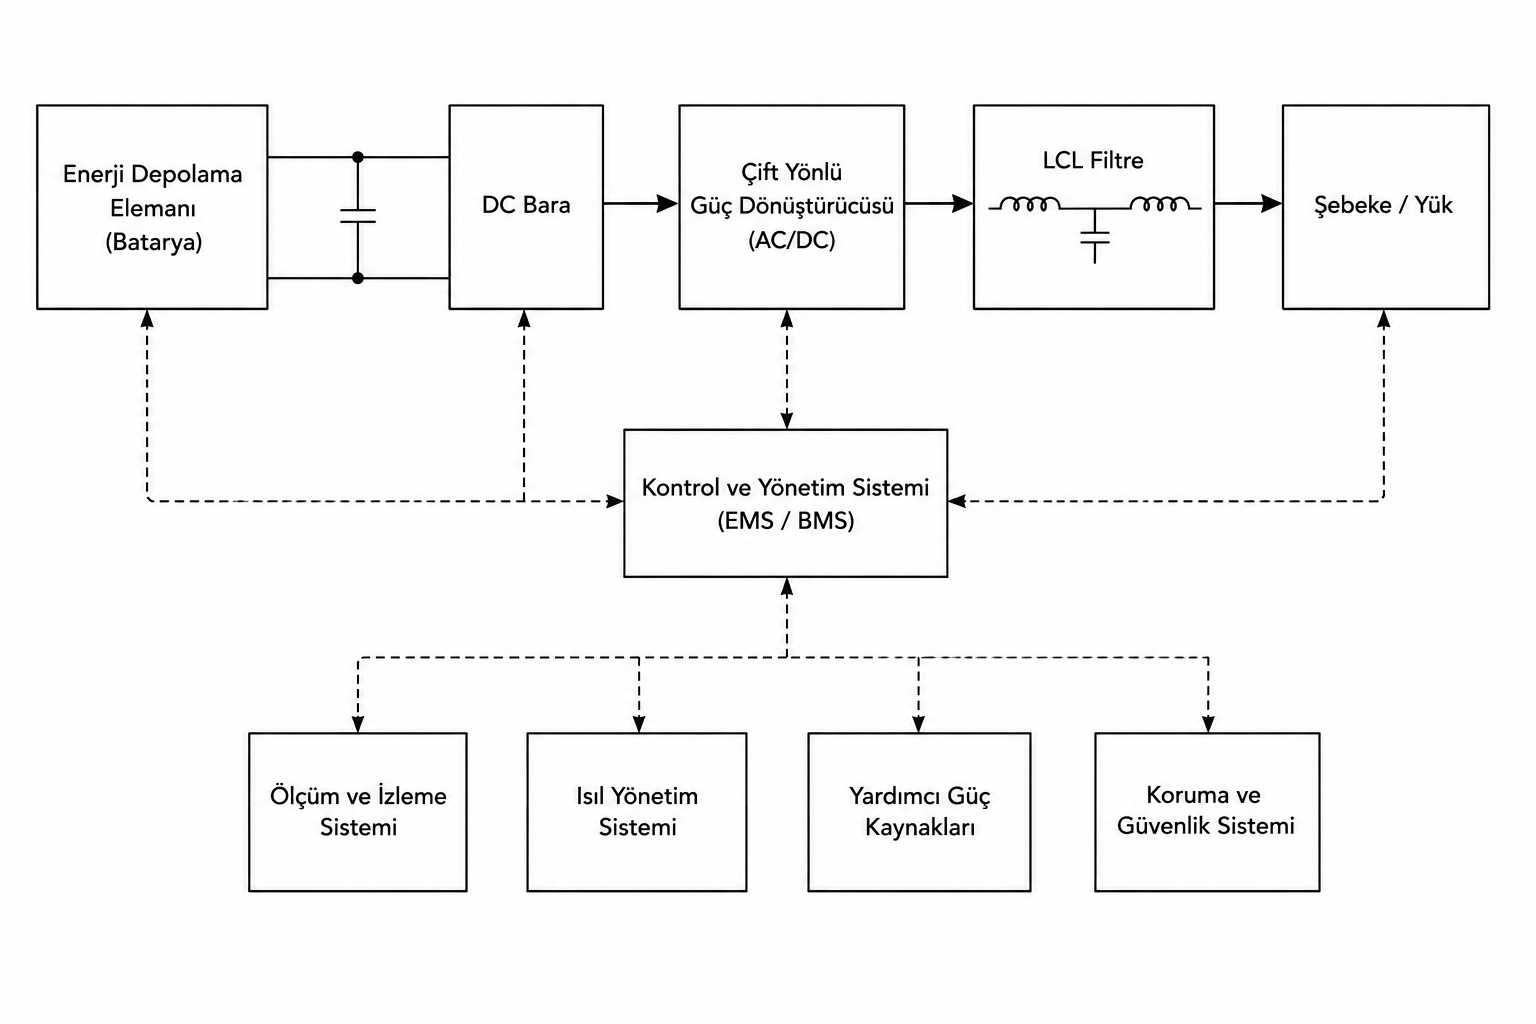
\includegraphics[width=0.96\textwidth]{literatur/gecici_eds_mimarisi_eski_tez.png}
  \caption{Şebeke bağlantılı bir enerji depolama sisteminin temel bileşenleri ve bilgi akışları.}
  \label{fig:eds-mimarisi}
\end{figure}

Geleneksel şebeke bağlantılı bir EDS'de batarya ile DA bara arasında çift yönlü DA/DA dönüştürücü, DA bara ile şebeke arasında evirici/doğrultucu ve hücreler arasında ayrı bir dengeleme devresi bulunabilir. Katların ayrılması, her işlev için bağımsız tasarım ve koruma olanağı sunar; karşılığında yarı iletken, manyetik eleman, sürücü, algılayıcı ve soğutma gereksinimini artırır. Sistem maliyeti çalışmalarında batarya paketi baskın kalem olsa da güç elektroniği donanımının maliyet, kayıp ve hacim üzerindeki etkisi ihmal edilemez \citep{Ramasamy2023,Lazard2024}. İşlevlerin ortak elemanlarla gerçekleştirilmesi, özellikle şarj ve deşarj kiplerinin aynı anda etkin olmadığı uygulamalarda donanım kullanım oranını yükseltme potansiyeli taşır.

\begin{table}[htbp]
  \centering
  \caption{Enerji depolama sistemi bileşenlerinin toplam sistem maliyetindeki tipik pay aralıkları \citep{Ramasamy2023,Lazard2024}.}
  \label{tab:eds-maliyet-dagilimi}
  \begin{tabular}{>{\raggedright\arraybackslash}p{0.67\textwidth} c}
    \toprule
    \textbf{Sistem bileşeni} & \textbf{Maliyet payı (\%)} \\
    \midrule
    Batarya paketi & 50--70 \\
    Güç dönüştürücüleri (evirici, PFC ve DA/DA) & 10--20 \\
    Batarya yönetim sistemi & 3--8 \\
    Enerji yönetim sistemi & 2--5 \\
    Isıl yönetim ve soğutma & 3--10 \\
    Koruma ve güvenlik sistemleri & 2--5 \\
    Yardımcı güç kaynakları ve haberleşme & 1--3 \\
    Mekanik yapı ve kablolama & 5--10 \\
    \bottomrule
  \end{tabular}
\end{table}

Aralıkların toplamı tek bir tasarımı temsil etmediği için Tablo~\ref{tab:eds-maliyet-dagilimi} içindeki yüzde sütunu doğrudan toplanmamalıdır; her satır farklı proje, güç ve tedarik koşullarından türetilen tipik bir aralıktır. Tablo, tezin GT-tipi mimarisindeki eleman paylaşımının neden ekonomik olarak anlamlı bir araştırma sorusu olduğunu gösterir; tek başına maliyet azalımını kanıtlamaz.

Batarya paketinin kullanılabilir ömrü; deşarj derinliği, hücre gerilimi, sıcaklık, akım oranı ve hücreler arası dengesizlikten etkilenir \citep{Vetter2005,Smith2017,Chen2021,Feng2018}. Şekil~\ref{fig:batarya-omur-guvenlik} altındaki deşarj derinliği--çevrim ömrü eğrisi ile güvenli çalışma bölgesi, belirli bir hücre kimyasının veri sayfası yerine literatürden uyarlanmış temsilî ilişkileri gösterdiğinden tasarım sınırı olarak kullanılmamalıdır.

\begin{figure}[htbp]
  \centering
  \begin{subfigure}[t]{0.49\textwidth}
    \centering
    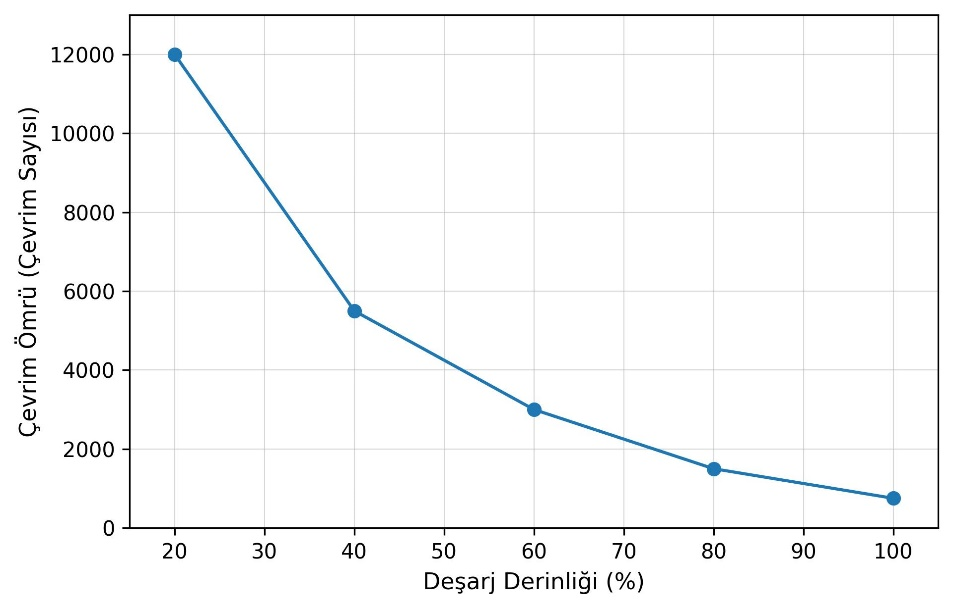
\includegraphics[width=\textwidth]{literatur/onceki_tez_dod_cevrim.jpg}
    \caption{Deşarj derinliği--çevrim ömrü ilişkisi.}
  \end{subfigure}\hfill
  \begin{subfigure}[t]{0.49\textwidth}
    \centering
    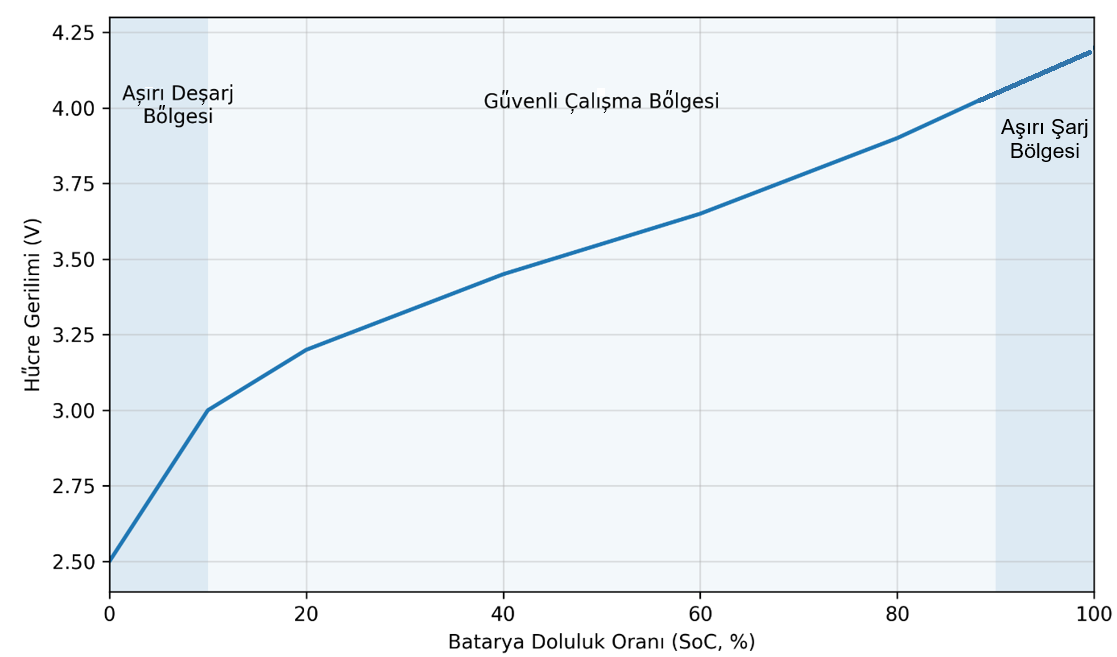
\includegraphics[width=\textwidth]{literatur/onceki_tez_guvenli_calisma.png}
    \caption{Temsilî gerilim ve doluluk sınırları.}
  \end{subfigure}
  \caption{Batarya ömrü ve güvenli işletim için kullanılan temsilî eğriler; \citet{Smith2017}, \citet{Chen2021} ve \citet{Feng2018} temel alınarak uyarlanmıştır.}
  \label{fig:batarya-omur-guvenlik}
\end{figure}

Hücre gerilimi, akım ve sıcaklık ölçümleri BYS denetleyicisine taşınır; koruma, kontaktör ve dengeleme komutları aynı karar katmanında üretilir. Tipik bir BYS'nin işlevsel mimarisi Şekil~\ref{fig:bys-mimarisi} üzerinde verilmiştir. Mimari, GT-tipi yapının hangi işlevleri ortak güç elemanlarına taşımayı hedeflediğini tanımlayan başvuru noktasıdır.

\begin{figure}[htbp]
  \centering
  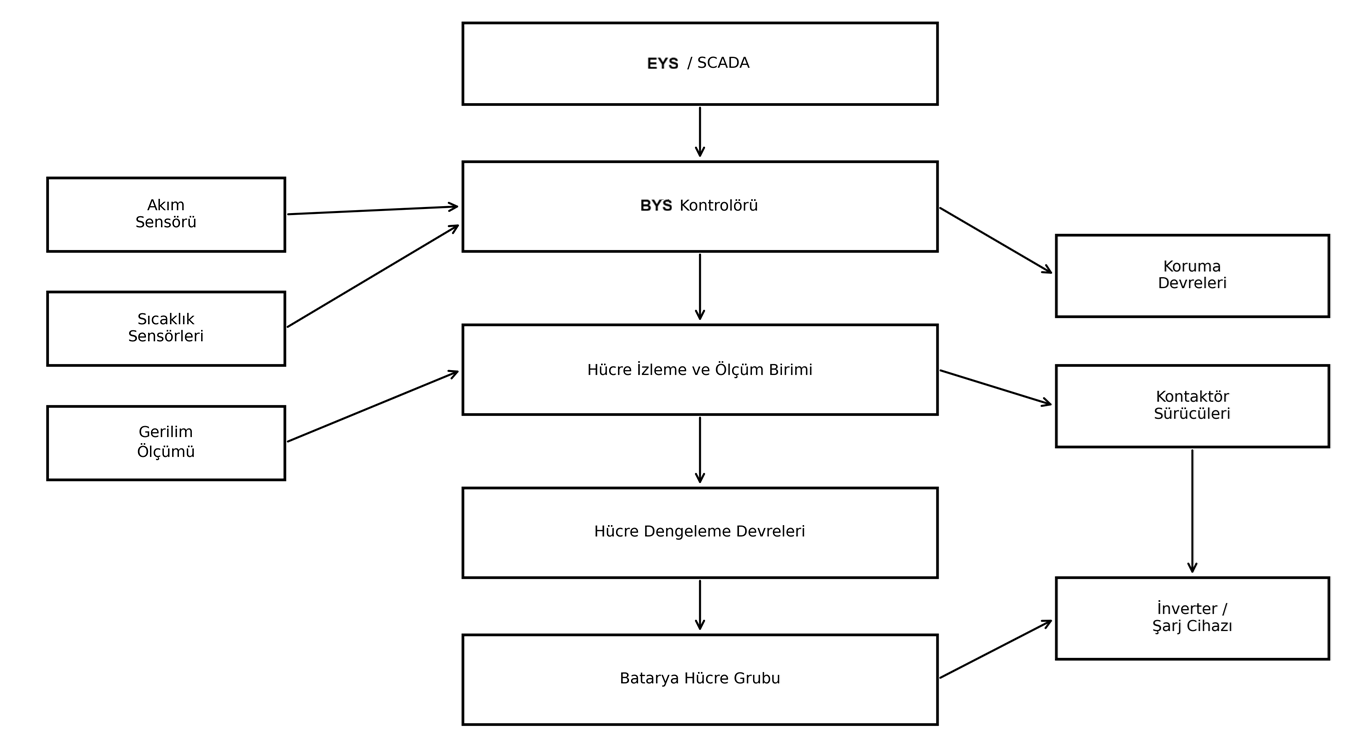
\includegraphics[width=0.94\textwidth]{literatur/onceki_tez_bys_mimarisi.png}
  \caption{Tipik bir batarya yönetim sisteminin ölçüm, karar, koruma ve dengeleme işlevleri.}
  \label{fig:bys-mimarisi}
\end{figure}

\begin{table}[htbp]
  \centering
  \caption{Geleneksel BYS ile hücre bazlı enerji yönetiminin işlevsel karşılaştırması.}
  \label{tab:bys-islev-karsilastirma}
  \setlength{\tabcolsep}{4pt}
  \begin{tabularx}{\textwidth}{>{\raggedright\arraybackslash}X >{\centering\arraybackslash}p{0.22\textwidth} >{\centering\arraybackslash}p{0.25\textwidth}}
    \toprule
    \textbf{İşlev} & \textbf{Geleneksel BYS} & \textbf{Hücre bazlı yönetim} \\
    \midrule
    Hücre izleme, koruma ve dengeleme & Var & Var \\
    Hücre bazlı şarj kontrolü & Sınırlı & Var \\
    Hücre bazlı deşarj kontrolü & Sınırlı & Var \\
    Ömür optimizasyonu & Dolaylı & Doğrudan \\
    \bottomrule
  \end{tabularx}
\end{table}

Tablo~\ref{tab:bys-islev-karsilastirma}'daki ``doğrudan'' ifadesi bir ömür kazancı yüzdesi değil, hücrenin güç yoluna ayrı ayrı müdahale edilebilmesini tanımlar. Sayısal ömür artışı ancak hücre kimyası, görev profili, sıcaklık ve yaşlanma testi birlikte verildiğinde ileri sürülebilir.

Seri bağlı hücre veya modüllerde kapasite, iç direnç, sıcaklık ve yaşlanma farklılıkları paket performansını en zayıf birimle sınırlandırabilir. Pasif dengeleme fazla enerjiyi dirençlerde harcarken aktif dengeleme kapasitör, endüktör, transformatör veya çift yönlü dönüştürücü üzerinden enerji aktarır \citep{Daowd2011,Khan2024}. Aktif yöntemler enerji kaybını azaltabilse de ilave anahtar ve manyetik eleman gereksinimi doğurur. Literatürdeki yeniden yapılandırılabilir batarya sistemleri, hücre veya modül bağlantılarını güç anahtarlarıyla değiştirerek dengeleme, arıza yalıtımı ve farklı terminal gerilimlerini aynı donanım üzerinden sağlamayı hedeflemektedir. Momayyezan ve arkadaşları, yüksek gerilimli batarya sisteminde yük besleme, geri kazanım, şarj ve modüller arası dengeleme kipleri için yarı iletkenleri ve bir endüktörü paylaşan bütünleşik bir dönüştürücü önermiş ve beş modüllü ölçekli prototiple çalışma kiplerini göstermiştir \citep{Momayyezan2016}. Farakhor ve arkadaşları ise yeniden yapılandırılabilir anahtar dizisini hücre düzeyindeki DA/DA dönüştürücülerle birleştirerek arızalı hücre yalıtımı, güç paylaşımı, şarj durumu ve sıcaklık dengelemesi sağlamış; yaklaşımı benzetim ve laboratuvar prototipiyle doğrulamıştır \citep{Farakhor2023}.

Pasif ve başlıca aktif dengeleme ailelerinin enerji aktarım elemanları Şekil~\ref{fig:dengeleme-yontemleri} üzerinde karşılaştırılmıştır. Şekil, yöntemlerin ayrıntılı devre tasarımından çok enerji yolundaki temel farkı göstermek amacıyla verilmiştir.

\begin{figure}[htbp]
  \centering
  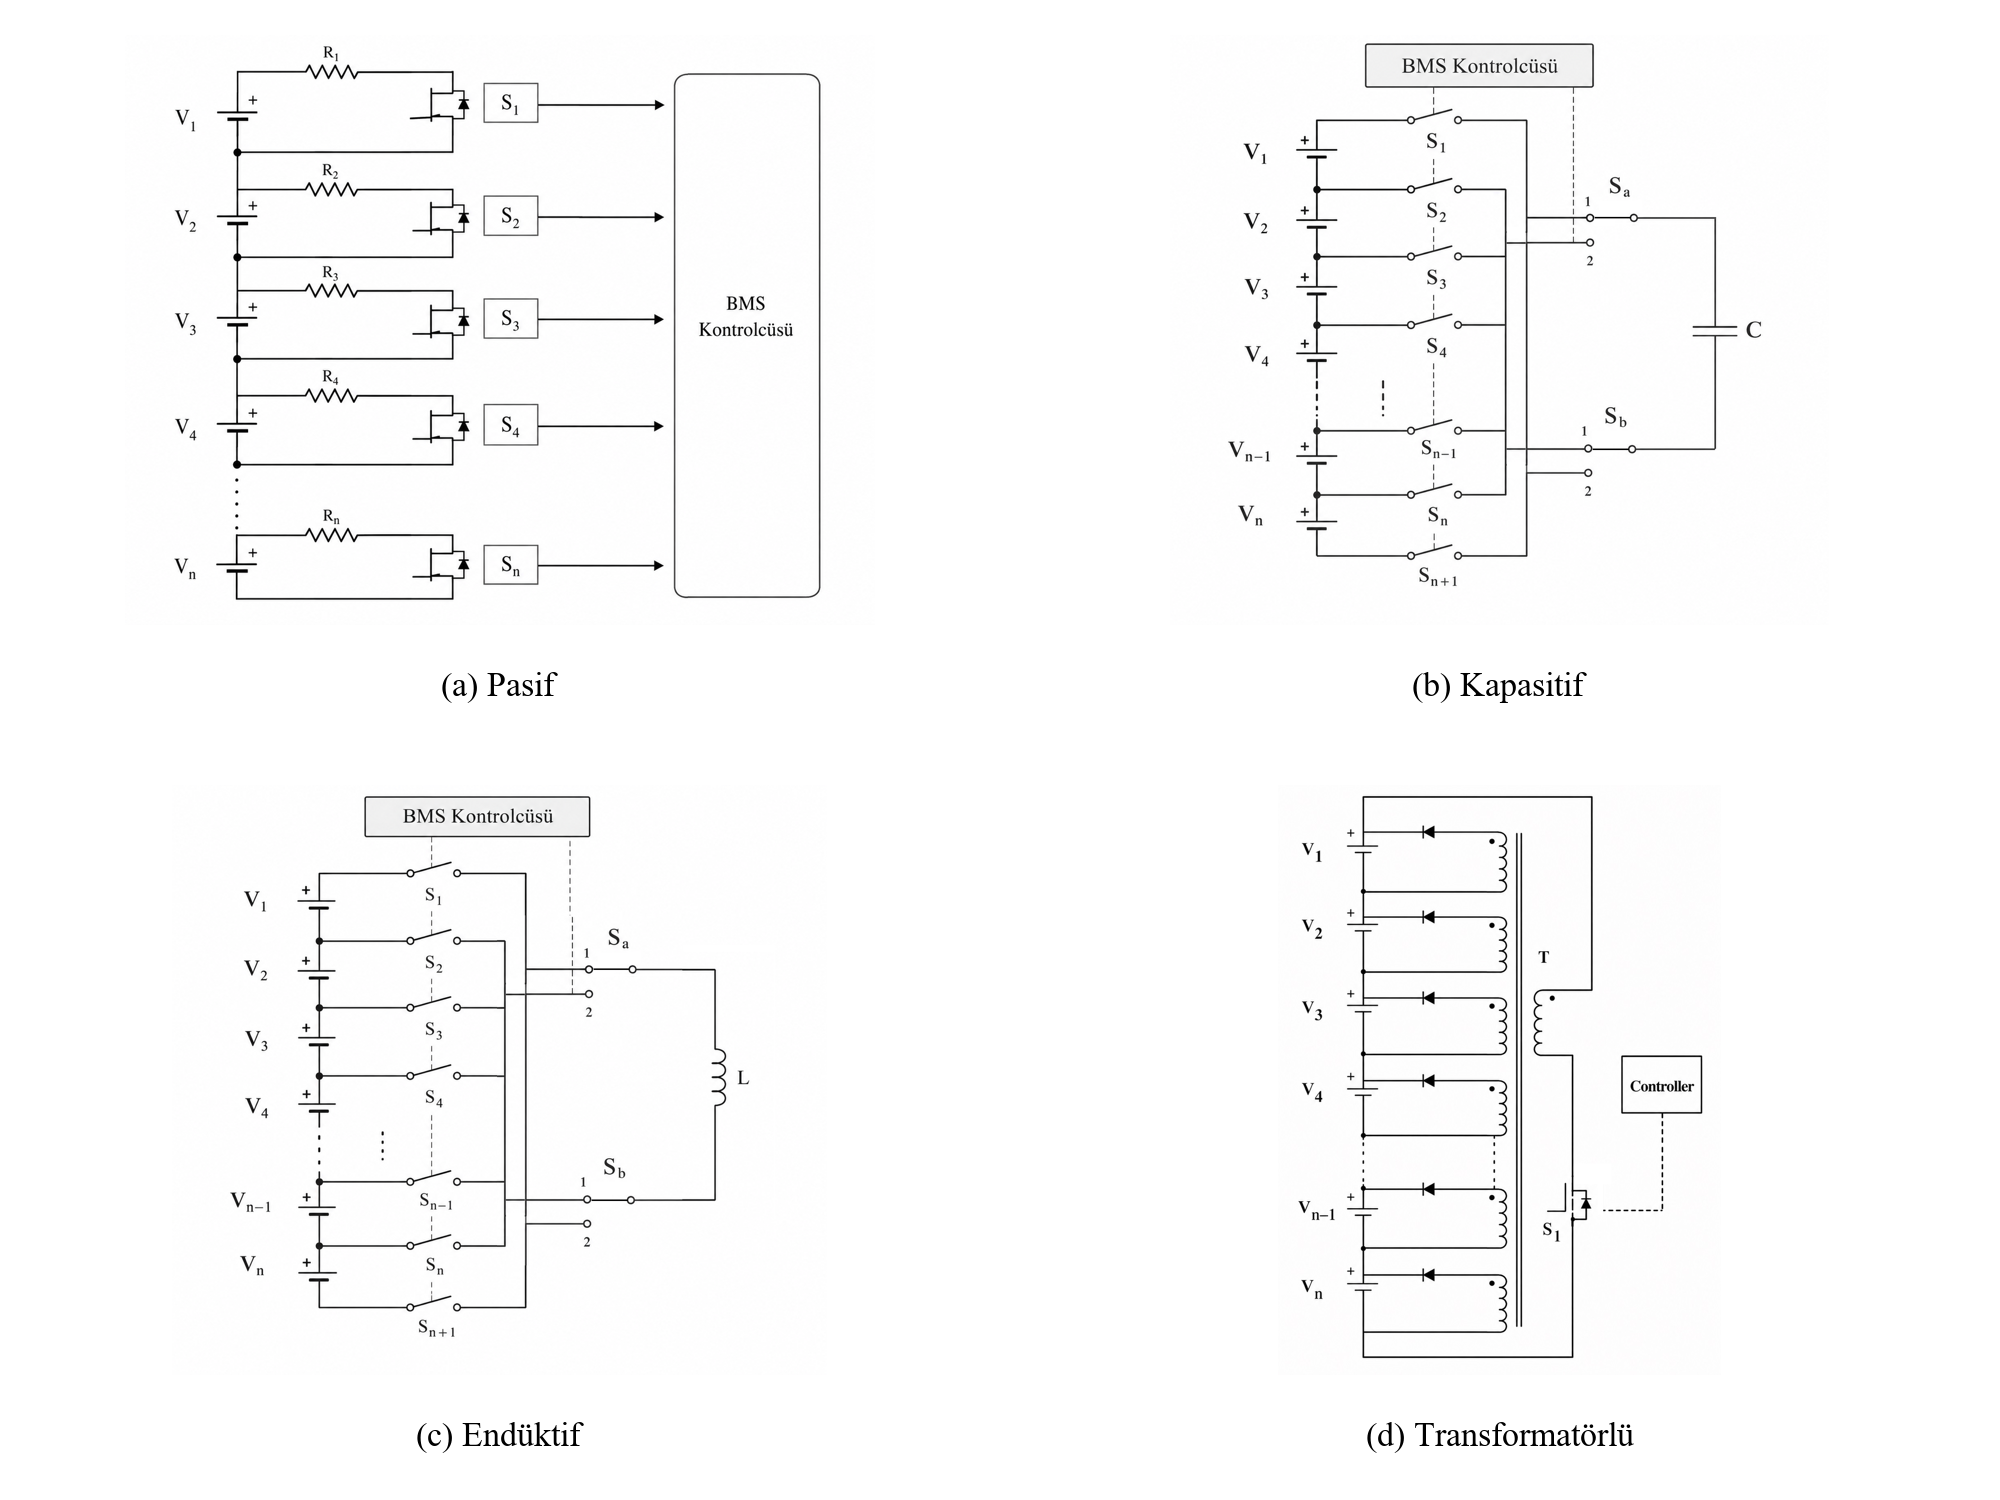
\includegraphics[width=0.94\textwidth]{literatur/gecici_dengeleme_yontemleri_bilesik.png}
  \caption{Pasif, kapasitif, endüktif ve transformatörlü hücre dengeleme yapılarının kavramsal karşılaştırması \citep{Daowd2011,Khan2024}.}
  \label{fig:dengeleme-yontemleri}
\end{figure}

Pasif dengeleme yönteminde, diğer hücrelere göre daha yüksek gerilim veya şarj durumuna sahip hücreye paralel bağlanan direnç üzerinden enerji harcanır. Anahtarın görev oranı hücreden çekilen dengeleme akımını belirler. Az sayıda eleman, basit denetim ve düşük maliyet başlıca avantajlardır. Fazla enerjinin ısıya dönüştürülmesi, soğutma gereksinimi ve düşük şarj durumundaki hücrelere enerji aktarılamaması ise yöntemin temel sınırlılıklarını oluşturur \citep{Daowd2011,Khan2024}.

Kapasitif dengelemede, anahtarlanan bir kapasitör farklı hücrelere sırasıyla bağlanarak gerilimi yüksek hücreden enerji alır ve gerilimi düşük hücreye aktarır. Manyetik eleman gerektirmeyen yapı, paketleme ve maliyet bakımından avantaj sağlayabilir. Dengeleme akımının hücreler arasındaki gerilim farkına bağlı olması, uzak hücreler arasında enerjinin birden fazla aktarım adımından geçmesi ve anahtar sayısının hücre sayısıyla artması dengeleme süresini uzatabilir \citep{Daowd2011,Khan2024}.

Endüktif dengeleme yönteminde enerji, anahtarlama sırasında bir endüktörde depolanır ve seçilen hücreye veya paket hattına kontrollü akım olarak aktarılır. Anahtarlama görev oranı üzerinden enerji akışının düzenlenebilmesi, kapasitif yönteme göre daha yüksek ve öngörülebilir dengeleme akımlarına olanak tanır. Endüktör, akım algılama, sürücü ve çift yönlü anahtarlama gereksinimleri devre ile denetim karmaşıklığını artırır \citep{Daowd2011,Khan2024}.

Transformatörlü yapılarda hücre sargıları ile ortak sargı arasındaki manyetik bağ; hücreden pakete, paketten hücreye veya seçilen hücreler arasında yalıtımlı enerji aktarımı sağlayabilir. Çoklu sargı yapısı farklı enerji yollarını desteklediği için hücre bazlı şarj ve deşarj işlevlerine geçiş bakımından önemlidir. Sargı sayısı, kaçak endüktans, sürme düzeni, hacim ve üretim maliyeti uygulama büyüdükçe belirleyici sınırlılıklara dönüşür \citep{Daowd2011,Khan2024}.

\begin{table}[htbp]
  \centering
  \caption{Başlıca hücre dengeleme ailelerinin nitel karşılaştırması \citep{Daowd2011,Khan2024}.}
  \label{tab:dengeleme-karsilastirma}
  \setlength{\tabcolsep}{3pt}
  \begin{tabularx}{\textwidth}{>{\raggedright\arraybackslash}p{0.20\textwidth} *{4}{>{\centering\arraybackslash}X}}
    \toprule
    \textbf{Yöntem} & \textbf{Enerji geri kazanımı} & \textbf{Maliyet} & \textbf{Karmaşıklık} & \textbf{Aktarım hızı} \\
    \midrule
    Pasif & Yok & Düşük & Düşük & Düşük \\
    Anahtarlamalı kapasitör & Var & Düşük--orta & Orta & Düşük--orta \\
    Endüktif & Var & Orta & Yüksek & Orta--yüksek \\
    Transformatörlü & Var & Yüksek & Yüksek & Uygulamaya bağlı \\
    \bottomrule
  \end{tabularx}
\end{table}

Nitel sınıflar topoloji, hücre sayısı ve dengeleme akımıyla değişebildiğinden Tablo~\ref{tab:dengeleme-karsilastirma} kesin bir sıralama değil, tasarım alanını özetleyen bir karşılaştırmadır. Dört yöntem birlikte değerlendirildiğinde tek bir dengeleme yapısının verim, hız, maliyet ve devre karmaşıklığı açısından her uygulamada üstün olmadığı görülür. Tezin GT-tipi mimari katkısı, dört dengeleme yönteminden birini genel olarak en iyi ilan etmek yerine, şarj--deşarj ve hücre yönetimi işlevlerinde mevcut yarı iletkenlerin yeniden görevlendirilmesine odaklanmaktadır. Şekil~\ref{fig:dengeleme-yontemleri}, ilerleyen bölümlerde sunulan işlev paylaşımının neden ayrı dengeleme donanımına alternatif oluşturabileceğini açıklayan kuramsal geçiş niteliğindedir.

Yeniden yapılandırılabilir sistemlerin esneklik kazancı yeni tasarım ödünleşimleri oluşturur. Anahtar sayısı yükseldikçe iletim kaybı, sürücü karmaşıklığı, yanlış anahtarlama riski ve güvenli kip geçişi gereksinimi büyür. Huang ve arkadaşlarının modüler yeniden yapılandırılabilir EDS çalışması, üç anahtarlı modül yapısıyla farklı bağlantıları ve arıza yalıtımını desteklerken işlev sayısı ile devre karmaşıklığı arasındaki ödünleşimi açıkça göstermiştir \citep{Huang2024}. Bütünleştirme, yalnızca eleman sayısını azaltma iddiasıyla değerlendirilemez; her çalışma kipi için akım yolu, eleman zorlanması, geçiş sırası, kayıp ve doğrulama düzeyi birlikte verilmelidir.

\section{Üç Seviyeli T-Tipi Dönüştürücünün Kuramsal Temeli}

EDS mimarisindeki güç dönüşüm katının verimi ve akım kalitesi, seçilen dönüştürücü topolojisine doğrudan bağlıdır; kesim, tezin odaklandığı T-tipi yapının literatürdeki yerini kurmaktadır. Gerilim kaynaklı iki seviyeli evirici, faz çıkışını DA baranın pozitif ve negatif uçları arasında anahtarlar. Yüksek anahtarlama frekansı akım dalgalanmasını ve filtre gereksinimini azaltırken anahtarlama kayıplarını artırır. Çok seviyeli dönüştürücüler, çıkış gerilimini daha küçük basamaklarla oluşturarak yarı iletken gerilim zorlanmasını, $dv/dt$ değerini ve filtreleme gereksinimini azaltmayı amaçlar \citep{Mohan2003,Holmes2003}. Üç seviyeli nötr nokta kenetlemeli (Neutral Point Clamped, NPC) yapı, sıfır seviyesini kenetleme diyotlarıyla üretirken T-tipi yapı nötr noktayı çift yönlü kontrollü bir anahtar kolu üzerinden faz çıkışına bağlar.

Bir T-tipi faz kolunda dış anahtarlar faz düğümünü DA baranın pozitif veya negatif yarısına, nötr anahtar çifti ise orta noktaya bağlar. İdeal anahtarlama durumları $+V_{\mathrm{dc}}/2$, $0$ ve $-V_{\mathrm{dc}}/2$ seviyelerini oluşturur. Pozitif ve negatif aktif durumlarda akım dış anahtarlar üzerinden, sıfır durumunda ise akım yönüne bağlı olarak nötr kol üzerinden akar. Nötr kol elemanlarının daha düşük gerilim sınıfında seçilebilmesi ile aktif durumdaki seri eleman sayısının NPC yapıya göre azalması, uygun gerilim ve anahtarlama frekansı aralığında iletim ve anahtarlama kayıpları açısından avantaj sağlayabilir.

T-tipi faz kolunun temel devre yapısı Şekil~\ref{fig:t-tipi-faz-kolu} üzerinde gösterilmiştir. Aynı devre, Bölüm~\ref{chap:sistem} içinde her anahtarlama durumu için akım yönleri işaretlenerek ayrıntılandırılacaktır.

\begin{figure}[htbp]
  \centering
  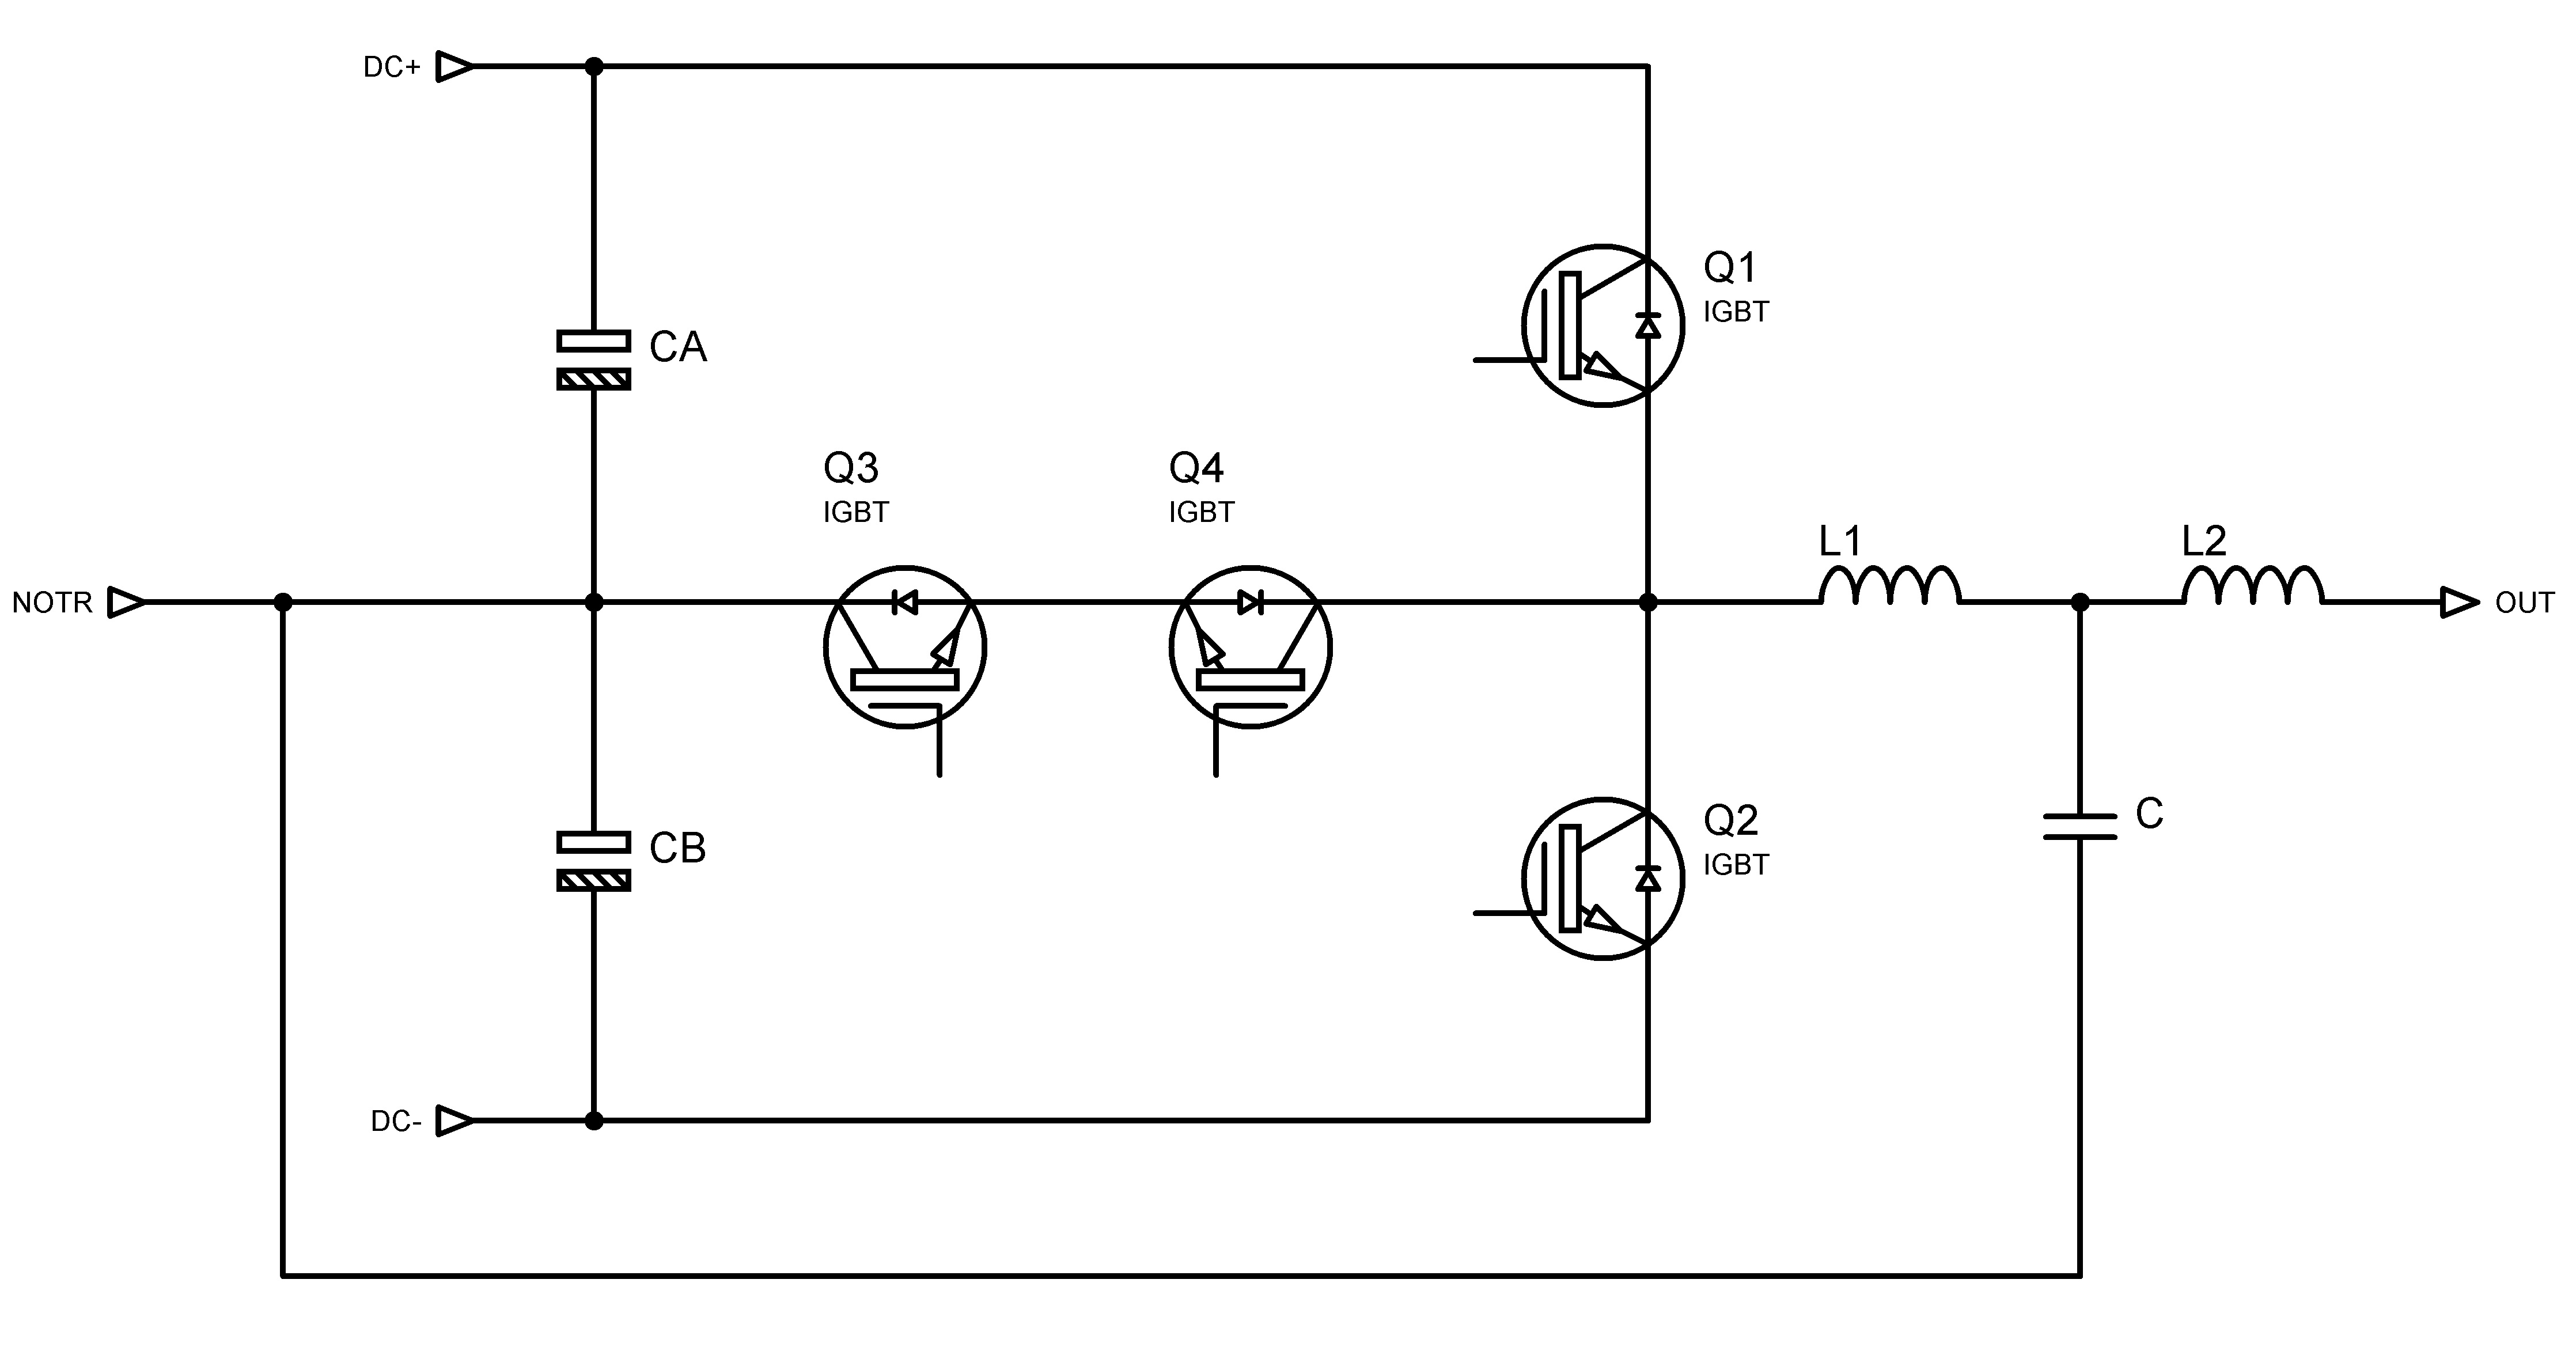
\includegraphics[width=0.88\textwidth]{literatur/gecici_t_tipi_faz_kolu_eski_tez.jpg}
  \caption{Üç seviyeli T-tipi eviricinin tek faz kolu ve çıkış filtresi.}
  \label{fig:t-tipi-faz-kolu}
\end{figure}

Schweizer ve Kolar, üç seviyeli T-tipi dönüştürücüyü iki seviyeli ve NPC seçenekleriyle yarı iletken kaybı, eleman alanı ve deneysel verim bakımından karşılaştırmış; düşük gerilim uygulamalarında yüksek anahtarlama frekansına rağmen yüksek verim elde edilebildiğini göstermiştir \citep{Schweizer2013}. Wang ve arkadaşlarının \SI{250}{\kilo\watt} SiC T-tipi evirici çalışması, çalışma aralıklarını ve anahtarlama geçişlerini ayrıntılı biçimde çözümleyerek ters iletimin eleman kayıpları üzerindeki etkisini modellemiş; \SI{25}{\kilo\watt\per\litre} güç yoğunluğu hedefli bir prototip sunmuştur \citep{Wang2020}. Hizarci ve arkadaşlarının \SI{25}{\kilo\watt}, \SI{15}{\kilo\hertz} şebeke bağlantılı T-tipi evirici üzerindeki iletilen emisyon çalışması ise topolojinin endüstriyel ölçekte filtre, kaçak akım ve elektromanyetik uyumluluk gereksinimleriyle birlikte ele alınması gerektiğini göstermektedir \citep{Hizarci2021}.

T-tipi topolojiye ilişkin çalışmaların önemli bölümü anma gücü, yüksek güç yoğunluğu, yarı iletken seçimi, nötr nokta dengesi ve modülasyon üzerine yoğunlaşmaktadır. Harmonik eleme amaçlı anahtarlama açıları ve üçüncü harmonik enjeksiyonu da DA bara kullanımını veya belirli gerilim harmoniklerini iyileştirmek amacıyla incelenmiştir \citep{Aghdam2013,Holmes2003}. Topoloji, modülasyon ve harmonik enjeksiyonu çalışmaları topolojinin genel verim ve dalga biçimi potansiyelini ortaya koymakla birlikte, şebekeye bağlı düşük akım koşulunda nötr kolun ters akım oluşturma mekanizmasını ve verim--THD ödünleşimini doğrudan merkezine almamaktadır.

\section{Fotovoltaik Çalışma Profili, Kısmi Yükte Verim ve Harmonik Bozulma}

T-tipi eviricinin düşük güç davranışının neden önemli olduğu, eviricinin fiilen hangi güç seviyelerinde çalıştığına bakılarak gerekçelendirilebilir. Fotovoltaik üretimin ışınım ve sıcaklığa bağlı değişimi, şebeke eviricisinin geniş bir güç aralığında çalışmasına neden olur. Şekil~\ref{fig:fv-calisma-profilleri}, temsilî günlük profil ile aylık ışınım dizisini ve iki diziden türetilen 144 çalışma noktasının güç dağılımını göstermektedir; grafikler MATLAB ile vektörel olarak üretilmiştir. PVGIS, konum, yönelim, eğim, sistem kaybı ve meteorolojik veri kümesi belirtilerek saatlik veya aylık üretim hesabı yapılmasına olanak tanır \citep{Taylor2025PVGIS}. Kullanılan diziler için böyle bir sorgunun konumu ve ham çıktısı mevcut olmadığından profiller ölçülmüş saha verisi değil, temsilî profil olarak adlandırılmıştır.

\begin{figure}[htbp]
  \centering
  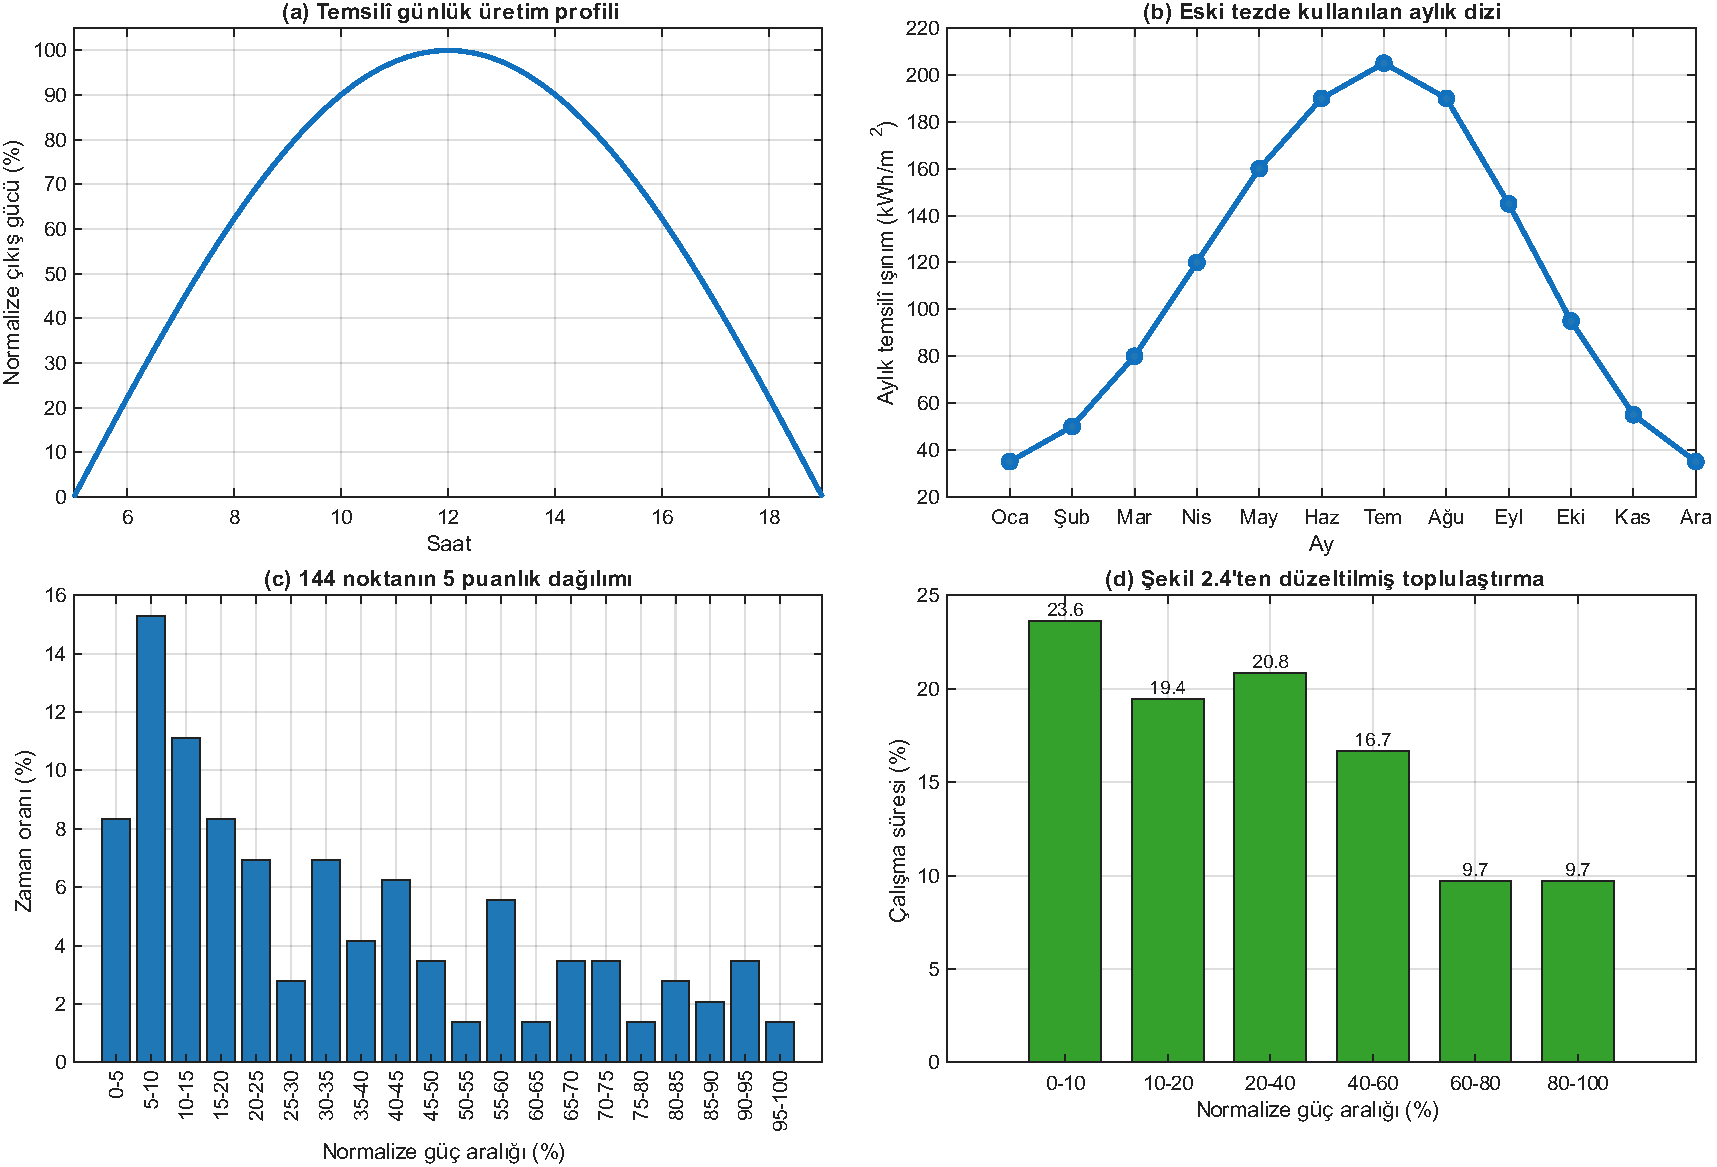
\includegraphics[width=\textwidth]{literatur/matlab_b2_guc_profilleri.pdf}
  \caption{Temsilî günlük ve aylık FV profilleri ile 144 çalışma noktasının MATLAB'da üretilen güç dağılımı. (d) paneli, (c) panelindeki nokta sayılarının güç sınıflarına yeniden gruplanmasıyla elde edilmiştir.}
  \label{fig:fv-calisma-profilleri}
\end{figure}

Günlük ve aylık diziler arasındaki çarpım bağı şu şekilde tanımlanmıştır. Saat indisi $h$, ay indisi $m$, boyutsuz gün içi normalize profil $p_d(h)$ ve aya bağlı temsilî ışınım seviyesi $G_m(m)$ ile gösterilsin. Aynı birimi $G_m$'den alan temsilî yıl--saat ışınımı $G_{\mathrm{tem}}(m,h)$
\begin{equation}
G_{\mathrm{tem}}(m,h)=G_m(m)\,p_d(h)
\label{eq:temsili-yil-saat-yuzeyi}
\end{equation}
biçiminde tanımlanır. Eşitlik~\eqref{eq:temsili-yil-saat-yuzeyi} ölçülmüş bir saha modeli değil, iki normalize dizinin çarpımıdır. Fotovoltaik gücün ışınımla orantılı olduğu basitleştirilmiş kabul altında $P_{\mathrm{tem}}(m,h)/P_n\approx G_{\mathrm{tem}}(m,h)/G_{\max}$ bağıntısı elde edilir; burada $P_{\mathrm{tem}}$ temsilî gücü, $P_n$ anma gücünü ve $G_{\max}$ yüzeydeki en büyük ışınımı gösterir. Temsilî örneklemdeki yaklaşık \SI{4}{\watt\per\metre\squared} ve \SI{200}{\watt\per\metre\squared} uçları, 50 katlık bir çalışma aralığına ve en düşük sıfırdan farklı noktanın tepe değerin yaklaşık \SI{2}{\percent}'sine karşılık geldiğine işaret etmektedir.

Şekil~\ref{fig:fv-calisma-profilleri}(c)'deki sayımlar 144 temsilî çalışma noktasına karşılık gelmektedir. İlk iki güç sınıfında toplam 34 nokta bulunması, eşit ağırlıklı ay--saat örneklemi içindeki noktaların \SI{23.6}{\percent}'sının anma gücünün \SI{10}{\percent}'undan düşük olduğunu gösterir. \SI{23.6}{\percent} oranı gerçek yıllık çalışma süresini değil, kullanılan temsilî örnekleme düzeninin dağılımını ifade etmektedir. Üç yıllık saha verisine dayanan bir çalışma, ışınımın önemli bir bölümünün düşük ve orta seviyelerde gerçekleştiğini; düşük ışınım ile evirici eşik kayıplarının sistem performansını etkilediğini göstermiştir \citep{Mondol2007}. Farklı iklim koşullarında yürütülen ağırlıklı verim incelemesi de yalnızca tepe veriminin saha davranışını temsil etmeye yetmediğini, evirici performansının değişen ışınım ve kısmi yük seviyeleriyle birlikte değerlendirilmesi gerektiğini ortaya koymuştur \citep{AbRahman2020}. Sonuç olarak \SI{23.6}{\percent} değeri evrensel bir yıllık oran olarak değil, düşük güç bölgesinin incelenmesini motive eden temsilî örneklem sonucu olarak kullanılmaktadır.

\begin{table}[htbp]
  \centering
  \caption{Temsilî 144 çalışma noktasının güç sınıfı dağılımı.}
  \label{tab:fv-guc-dagilimi}
  \begin{tabular}{ccc}
    \toprule
    \textbf{Çıkış gücü ($\%P_n$)} & \textbf{Nokta sayısı} & \textbf{Temsilî oran (\%)} \\
    \midrule
    0--10 & 34 & 23,6 \\
    10--20 & 28 & 19,4 \\
    20--40 & 30 & 20,8 \\
    40--60 & 24 & 16,7 \\
    60--80 & 14 & 9,7 \\
    80--100 & 14 & 9,7 \\
    \midrule
    Toplam & 144 & 100,0 \\
    \bottomrule
  \end{tabular}
\end{table}

Yıllık enerji verimi yalnızca tepe verimle belirlenmediğinden Avrupa ve CEC ağırlıklı verim tanımları, farklı yük noktalarındaki dönüşüm verimlerini belirli katsayılarla birleştirir. Alt indis $x$, anma gücünün yüzde $x$ noktasını; $\eta_x$ ise aynı noktadaki dönüşüm verimini göstersin. Avrupa ağırlıklı verimi
\begin{equation}
\eta_{\mathrm{EU}}=0{,}03\eta_{5}+0{,}06\eta_{10}+0{,}13\eta_{20}+0{,}10\eta_{30}+0{,}48\eta_{50}+0{,}20\eta_{100}
\label{eq:eta-eu}
\end{equation}
ve CEC ağırlıklı verimi
\begin{equation}
\eta_{\mathrm{CEC}}=0{,}04\eta_{10}+0{,}05\eta_{20}+0{,}12\eta_{30}+0{,}21\eta_{50}+0{,}53\eta_{75}+0{,}05\eta_{100}
\label{eq:eta-cec}
\end{equation}
olarak tanımlanır \citep{Sera2008,Sandia2015}. Eşitlik~\eqref{eq:eta-eu} ve Eşitlik~\eqref{eq:eta-cec} içindeki katsayıların toplamı birdir; iki ifade de boyutsuz ağırlıklı ortalamadır. Deneysel test düzenekleri ve standartlaştırılmış protokoller, verimin güç seviyesi, giriş gerilimi ve MPPT koşullarıyla birlikte ölçülmesini öngörür \citep{Sera2008,Sandia2015}. İzmir ışınım verilerine dayalı çalışma da bölgesel güç dağılımının ağırlık katsayılarını değiştirebildiğini göstermiştir \citep{Ongun2013}.

\begin{table}[htbp]
  \centering
  \caption{Avrupa ve CEC ağırlıklı verim katsayıları \citep{Sera2008,Sandia2015}.}
  \label{tab:agirlikli-verim-katsayilari}
  \begin{tabular}{c*{6}{c}}
    \toprule
    \textbf{Yöntem} & \multicolumn{6}{c}{\textbf{Güç seviyesi ve ağırlık katsayısı}} \\
    \midrule
    Avrupa & $5:0{,}03$ & $10:0{,}06$ & $20:0{,}13$ & $30:0{,}10$ & $50:0{,}48$ & $100:0{,}20$ \\
    CEC & $10:0{,}04$ & $20:0{,}05$ & $30:0{,}12$ & $50:0{,}21$ & $75:0{,}53$ & $100:0{,}05$ \\
    \bottomrule
  \end{tabular}
\end{table}

Kısmi yük davranışının verim ve harmonik boyutları Şekil~\ref{fig:fv-verim-thd-profilleri} üzerinde birlikte verilmiştir. Paneller (a) ve (c) genel eğilimi gösteren tipik dizilerdir; belirli bir ürünün doğrulanmış veri sayfası veya yeni deney sonucu değildir. Paneller (b) ve (d) aynı dizilerin 144 temsilî çalışma noktasına uygulanmasından elde edilen ikincil hesaplardır ve tez katkısının performans kanıtı olarak kullanılmamaktadır.

\begin{figure}[H]
  \centering
  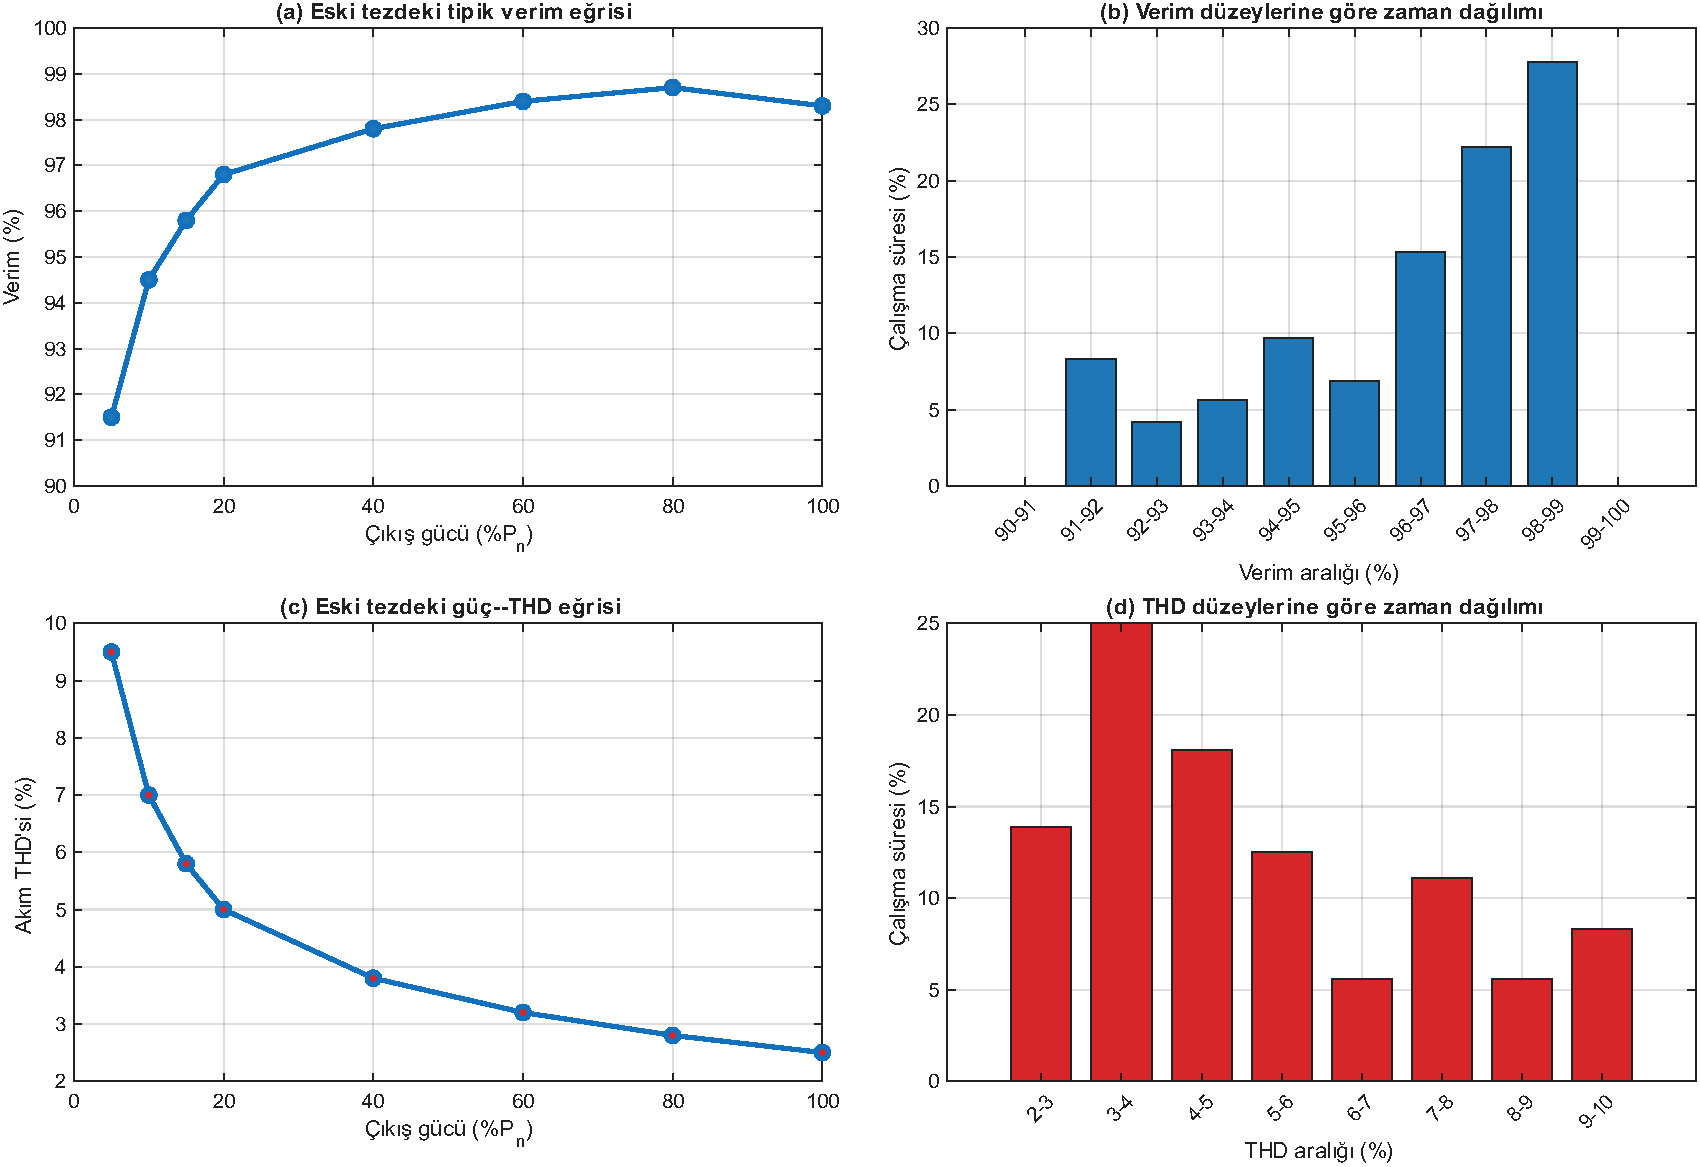
\includegraphics[width=\textwidth]{literatur/matlab_b2_verim_thd_profilleri.pdf}
  \caption{Tipik kısmi yük verim ve THD eğrileri ile bunlardan türetilen temsilî zaman dağılımlarının MATLAB'da vektörel üretimi.}
  \label{fig:fv-verim-thd-profilleri}
\end{figure}

Şekil~\ref{fig:fv-verim-thd-profilleri}(a)'daki dizide verim, \SI{5}{\percent} yükte yaklaşık \SI{91.5}{\percent}, \SI{10}{\percent} yükte \SI{94.5}{\percent} ve \SI{80}{\percent} yükte \SI{98.7}{\percent} düzeyindedir. Aynı şeklin (c) panelinde akım THD'si \SI{5}{\percent} yükte \SI{9.5}{\percent}, \SI{20}{\percent} yükte \SI{5.0}{\percent} ve anma gücünde \SI{2.5}{\percent} olarak verilmiştir. Şeklin bölümdeki amacı, yalnızca tepe veriminin ve anma gücündeki THD'nin yıllık davranışı açıklamaya yetmediğini ortaya koymaktır.

Düşük güçte THD artışının dış literatür kanıtı, \citet{Chicco2009} tarafından raporlanan günlük güç ve akım THD kaydıyla Şekil~\ref{fig:chicco-guc-thd} üzerinde gösterilmiştir. Sabah ve akşam düşük güç bölgelerinde THD'nin yükselmesi, tezin kısmi yük odağını destekler; belirli harmoniklerin T-tipi nötr kol mekanizmasından kaynaklandığını tek başına kanıtlamaz.

\begin{figure}[H]
  \centering
  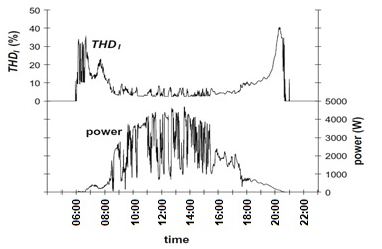
\includegraphics[width=0.62\textwidth]{literatur/chicco2009_guc_thd.png}
  \caption{\SI{5}{\kilo\watt} sınıfındaki bir FV eviricinin gün içi çıkış gücü ve akım THD'si; \citet{Chicco2009}'dan alınmıştır.}
  \label{fig:chicco-guc-thd}
\end{figure}

Şebekeye bağlı \SI{10}{\kilo\watt} sınıfındaki ticari bir eviricinin sabah devreye giriş kaydı Tablo~\ref{tab:ticari-evirici-thd} üzerinde verilmiştir. Cihaz seri numarası, güç analizörü, örnekleme penceresi, şebeke gerilimi ve ham dosya mevcut olmadığından satırlar yeni deney kanıtı değil, düşük güç bölgesinin önemini gösteren ve ham kaydı belgelenmemiş bir gözlem kaydıdır.

\begin{table}[H]
  \centering
  \caption{Ticari bir eviricinin sabah devreye girişinde kaydedilen güç ve akım THD değerleri; ham ölçüm dosyası ve protokolü belgelenmemiş motivasyon kaydı.}
  \label{tab:ticari-evirici-thd}
  \begin{tabular}{lrrr}
    \toprule
    \textbf{Zaman} & \textbf{Güç (W)} & \textbf{Güç ($\%P_n$)} & \textbf{THD (\%)} \\
    \midrule
    Devreye ilk giriş & 100 & 1,00 & 400 \\
    07:50 & 500 & 5,00 & 34 \\
    08:00 & 580 & 5,80 & 27 \\
    08:10 & 729 & 7,29 & 26 \\
    08:35 & 1060 & 10,60 & 17 \\
    08:50 & 1320 & 13,20 & 14 \\
    09:05 & 1450 & 14,50 & 14 \\
    09:18 & 1720 & 17,20 & 13 \\
    09:26 & 1880 & 18,80 & 9 \\
    09:42 & 2200 & 22,00 & 8 \\
    \bottomrule
  \end{tabular}
\end{table}

\begin{figure}[H]
  \centering
  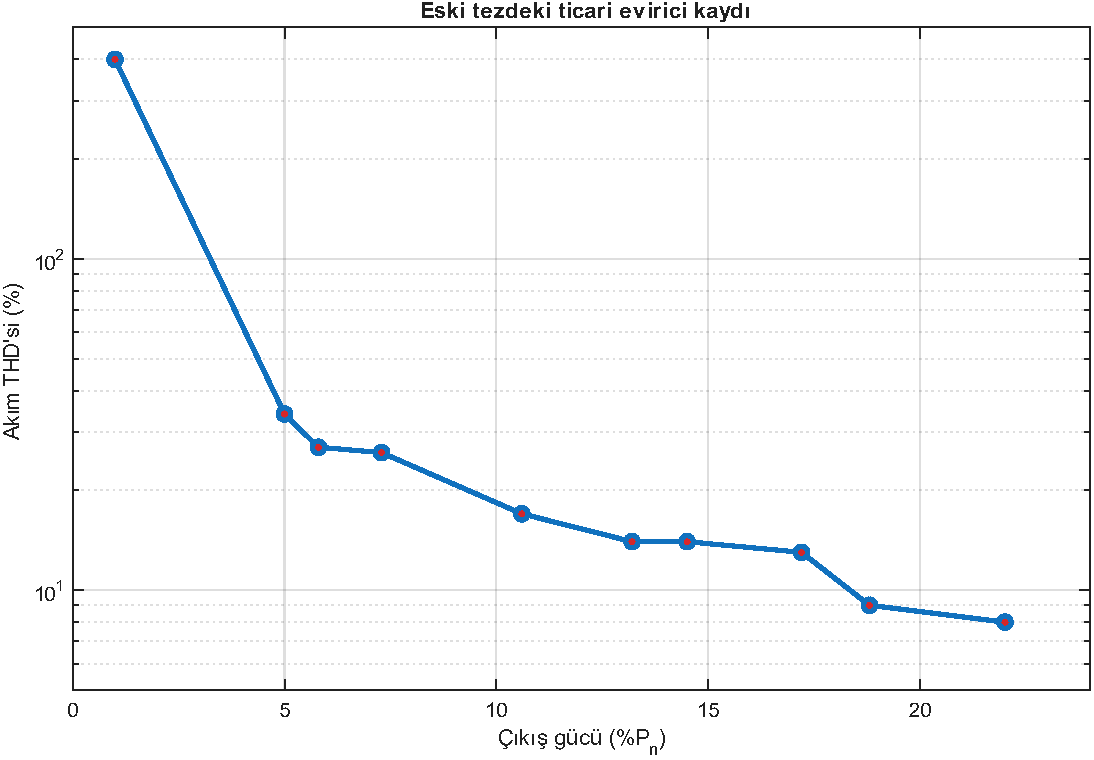
\includegraphics[width=0.84\textwidth]{literatur/matlab_b2_ticari_evirici_thd.pdf}
  \caption{Tablo~\ref{tab:ticari-evirici-thd}'deki kaydın MATLAB'da çizimi; düşey eksen logaritmiktir; veri, ham kaydı belgelenmemiş motivasyon kaydıdır.}
  \label{fig:ticari-evirici-thd}
\end{figure}

Şekil~\ref{fig:ticari-evirici-thd}, kayıttaki doğrusal olmayan azalmayı logaritmik eksende görünür hâle getirmektedir: akım THD'si anma gücünün \SI{1}{\percent}'inde \SI{400}{\percent} iken \SI{22}{\percent}'sinde \SI{8}{\percent} düzeyine iner. Grafiğin bölümdeki görevi, devreye giriş ve düşük güç test noktalarının yalnızca anma gücündeki tek bir ölçümle temsil edilemeyeceğini göstermektir; ham kaydı belgelenmemiş bir gözlem olarak önerilen anahtarlama yönteminin başarısını kanıtlamaz, laboratuvar deneylerinin düşük güç noktasında yürütülmesini gerekçelendirir.

Temsilî FV profili ile ticari evirici kaydının tezdeki rolü motivasyonla sınırlıdır. Şekil~\ref{fig:fv-calisma-profilleri} ve Tablo~\ref{tab:fv-guc-dagilimi} belirli bir konum için sorgulanmış PVGIS ham çıktısına, Tablo~\ref{tab:ticari-evirici-thd} ise cihaz modeli, analizör ve ölçüm penceresi belgelenmiş bir ham kayda dayanmamaktadır. İki içerik, düşük güç bölgesinin işletmede sık görüldüğünü ve düşük güçte akım THD'sinin yükseldiğini literatürle birlikte nitel olarak destekler; tezin verim ve THD bulgularına sayısal girdi oluşturmaz. Saha profili ve ham kayıt eksikliği Bölüm~\ref{chap:sonuc} içinde sınırlılık olarak yer almaktadır.

Düşük güçte sürücü, kontrol, anahtarlama ve manyetik elemanların güce zayıf bağlı kayıpları toplam çıkışa oranla büyür. Şebeke akımının küçük olması, ölü zaman ve anahtar doğrusal olmayanlıklarının temel bileşene oranını da artırır. Saha ve laboratuvar ölçümleri, FV eviricilerde akım dalga biçimi bozulmasının güç seviyesi ve şebeke gerilim kalitesiyle değiştiğini göstermektedir \citep{Kjaer2005,Chicco2009}. Harmonik sınırları bağlantı gücü ve standart kapsamına göre tanımlansa da yalnızca toplam THD değerine bakılması, hangi harmonik bileşenin hangi fiziksel mekanizmadan kaynaklandığını açıklamaz \citep{IEC61000}.

Ters akım problemi, senkron alçaltıcı dönüştürücünün hafif yük davranışı üzerinden açıklanabilir. Sürekli iletim kipinde (Continuous Conduction Mode, CCM) alt anahtar akım sıfırı geçtikten sonra açık tutulursa endüktör akımı negatif yönde büyür ve kaynak ile yük arasında yararlı güç üretmeyen enerji dolaşımı oluşur. Diyot benzetimi veya süreksiz iletim kipinde (Discontinuous Conduction Mode, DCM) senkron anahtar akım sıfıra yaklaşırken kapatılarak negatif akım engellenir \citep{Erickson2001,Mohan2003}. Chen ve arkadaşları, hafif yükte diyot benzetimi ile sürekli iletim kipini kayıp bileşenleri bakımından karşılaştırmış; ters akımın engellenmesinin RMS akımı ve iletim kaybını azaltabildiğini, ancak anahtarın ideal olmayan sıfır akım algılama anının yeni kayıplar oluşturabileceğini göstermiştir \citep{Chen2010}.

Diyot benzetimi ile sürekli iletim kipindeki endüktör akımları Şekil~\ref{fig:de-ccm-akim} üzerinde karşılaştırılmıştır. Sürekli iletim kipindeki akımın sıfırın altına geçmesi, tezde nötr anahtar üzerinden oluşan ters akımın açıklanmasında kullanılan temel benzerliği oluşturmaktadır.

\begin{figure}[htbp]
  \centering
  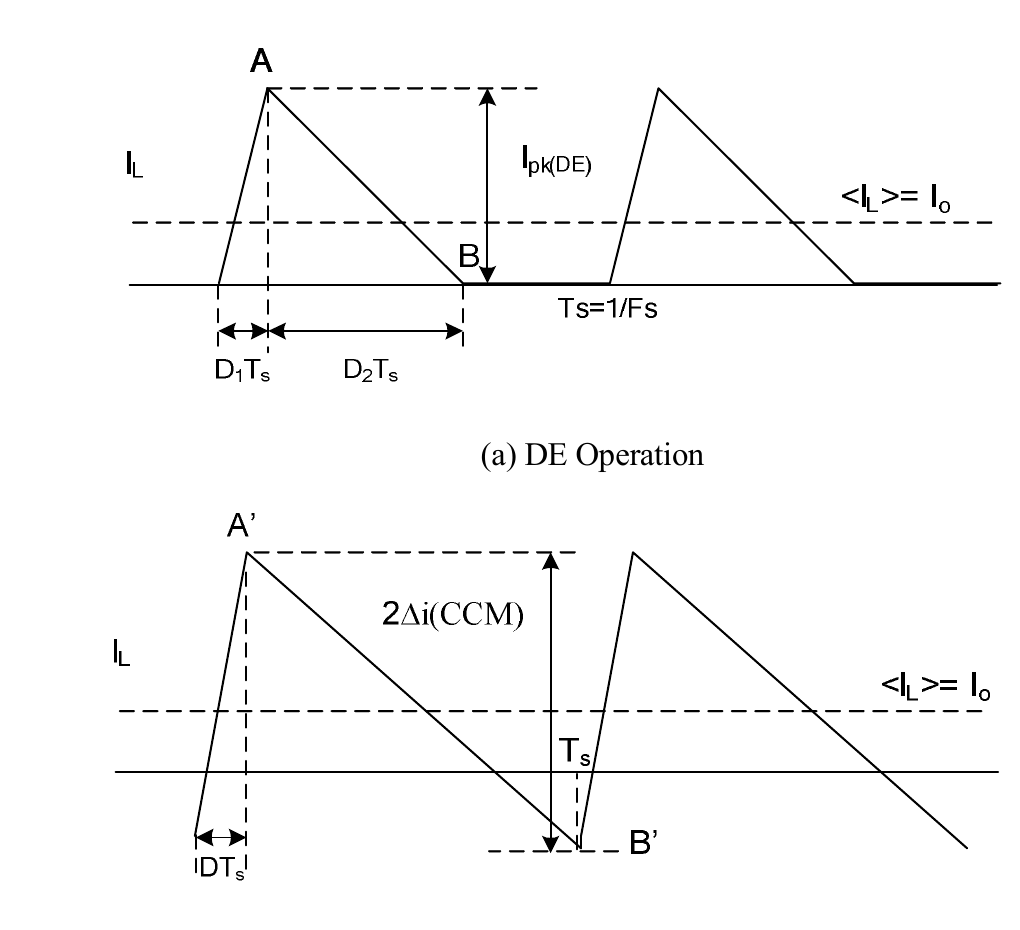
\includegraphics[width=0.68\textwidth]{literatur/gecici_de_ccm_akim_chen34.png}
  \caption{Diyot benzetimi (DE) ve sürekli iletim (CCM) kiplerinde endüktör akımının karşılaştırılması; Chen ve arkadaşlarından alınmıştır \citep{Chen2010}.}
  \label{fig:de-ccm-akim}
\end{figure}

Şebekeye bağlı T-tipi eviricide sıfır gerilim durumunu oluşturan nötr kol, akımın işaret değiştirmesine izin verdiğinde benzer bir senkron alçaltıcı davranışı gösterebilir. Nötr anahtarın susturulması ters akım yolunu keserken faz düğümünün doğal diyot yolları üzerinden farklı bir gerilim durumuna geçmesine neden olur. Kayıp azalması ile anahtarlama darbe dizisinin değişmesi böylece aynı fiziksel müdahalenin iki sonucudur. Literatürdeki genel süreksiz iletim bilgisi ters akımı açıklamak için gerekli kuramsal temeli sağlasa da T-tipi faz kolunda oluşan gerilim hatasının üçüncü harmonik etkisini ve şebeke akım kontrolüyle etkileşimini tek başına açıklamamaktadır.

Senkron alçaltıcıdaki CCM/DCM ayrımının T-tipi nötr kol üzerindeki karşılığı, tezin benzetim modelinden aynı zaman tabanında üretilmiştir. Nötr anahtar susturmada $Q_1$--$Q_4$ kapı komutları Şekil~\ref{fig:s2-kapi-isaretleri} üzerinde, klasik anahtarlama ile susturmanın kutup gerilimi ve şebeke akımı Şekil~\ref{fig:s1-s2-kalibre-dalga} üzerinde verilmiştir. Susturmalı çalışmada $L_1$ akımı söndüğünde kutup gerilimi üç seviyeden hiçbirinde bulunmaz; sürmesiz aralık, Şekil~\ref{fig:de-ccm-akim} içindeki diyot benzetimi kipinin sıfır akım aralığına karşılık gelir. $L_1$ akımının her anahtarlama çevriminde sıfıra oturduğu aralıklar Şekil~\ref{fig:susturma-l1-yakin} üzerinde, sürmesiz aralığın zaman oranı ve köprü davranışına etkisi Kesim~\ref{sec:dusuk-akim-modelleme} içinde gösterilmiştir.

\section{Şebeke Akım Kontrolü ve İleri Besleme Yaklaşımları}

Düşük güç mekanizması tek başına devre düzeyinde çözülemez; ters akımı kesen her müdahale, akım kontrol döngüsünün gördüğü bitkiyi de değiştirir. Kesim, tezin kompanzasyon katkısının dayandığı kontrol literatürünü özetlemektedir. Şebekeye bağlı bir eviricide akım denetleyicisi, referans akım ile ölçülen akım arasındaki hatadan modülasyon gerilimi üretir. Senkron referans çerçevesi, durağan eksen PI kontrolü ve oransal-rezonans (Proportional-Resonant, PR) kontrolü yaygın seçenekler arasındadır. PR denetleyici, temel frekansta yüksek kazanç sağlayarak sinüzoidal referansın kalıcı durum hatasını azaltabilir; seçili harmoniklerde ek rezonans kolları da kullanılabilir \citep{Teodorescu2006PR,Teodorescu2011}. Faz kilitlemeli döngü (Phase-Locked Loop, PLL) veya eşdeğer bir eşzamanlama yapısı, şebeke faz ve frekans bilgisini üretir; tek fazlı sistemlerde ortogonal işaret üretimi ve dijital gecikmeler tasarımın parçasıdır \citep{Blaabjerg2006,Zhou2018}.

LCL filtre, daha küçük toplam endüktansla yüksek frekanslı anahtarlama bileşenlerini zayıflatabilmesine karşılık rezonans tepesi oluşturur. Pasif sönümleme direnç kaybı doğururken aktif sönümleme ölçülen akım veya gerilim işaretlerinden sanal empedans etkisi üretir. PR denetleyici ile LCL aktif sönümlemenin birlikte tasarımı, kapalı çevrim kutupları ve kararlılık marjları dikkate alınarak yapılmalıdır \citep{Zhang2014PR}. Şebeke gerilimi ileri beslemesi, ortak bağlantı noktasındaki bozucu gerilimin akıma taşınmasını azaltmak için modülasyon girişine ölçülen gerilimden türetilen bir terim ekler. Lu ve arkadaşları, dijital gecikmenin ileri besleme yolunu LCL rezonansı üzerinde aktif sönümleme veya negatif sönümleme üretebilen dinamik bir elemana dönüştürebildiğini göstermiştir \citep{Lu2016}. Zayıf şebeke koşullarını inceleyen Wang ve arkadaşları da şebeke empedansına bağlı pozitif geri besleme etkisinin faz marjını azaltabileceğini ve ileri besleme kanalının frekans seçici biçimde tasarlanması gerektiğini ortaya koymuştur \citep{Wang2024}.

Anahtar ölü zamanı, snubber ve parazitik kapasiteler de komut edilen gerilim ile gerçekleşen faz gerilimi arasında akım yönüne bağlı hata oluşturur. Zhang ve Xu, parazitik kapasitelerin anahtarlama kenarlarını sonlu eğimli hâle getirdiğini ve klasik darbe tabanlı ölü zaman kompanzasyonunun özellikle küçük akımlarda yetersiz kalabildiğini deneysel olarak göstermiştir \citep{Zhang2014Deadtime}. Düşük güç harmonikleri, yalnızca denetleyici bant genişliğinin değil; modülasyon, anahtar geçişi, akım yönü ve şebeke geriliminin ortak sonucudur.

Sin\textsuperscript{3} tabanlı yaklaşımın literatürdeki yerini doğru kurabilmek için üçüncü harmonik enjeksiyonu ile bozucu bastırma amaçlı ileri besleme ayrılmalıdır. Klasik üçüncü harmonik enjeksiyonu, faz referanslarına ortak mod bileşeni ekleyerek DA bara kullanım oranını artırmayı veya belirli anahtarlama harmoniklerini düzenlemeyi hedefler \citep{Holmes2003,Aghdam2013}. Tezde ele alınan Sin\textsuperscript{3} terimi ise nötr anahtar susturma yönteminin oluşturduğu üçüncü harmonik etkisine karşı, ölçülen şebeke işaretinden $\sin^3(\theta)=[3\sin(\theta)-\sin(3\theta)]/4$ özdeşliğiyle üretilen bir şekillendirme bileşenidir. Fourier gösterimi matematiksel temeli sağlarken terimin modülasyon girişine eklenmesi onu hata sinyalinden türetilen bağımsız bir geri besleme denetleyicisi yapmaz \citep{Oppenheim1997}.

İdeal doğrusal ve doyumsuz modelde dışsal ileri besleme terimi kapalı çevrimin karakteristik paydasını değiştirmeyebilir. Gerçek dönüştürücüde örnekleme, PWM gecikmesi, LCL rezonansı, sınırlayıcılar ve çalışma noktasına bağlı anahtarlama doğrusal olmayanlıkları ideal ayrımı sınırlar. Periyodik çalışma noktaları çevresindeki frekans bağlaşımının incelenmesi gerektiğinde doğrusal zamanla periyodik modeller ve harmonik transfer fonksiyonları (Harmonic Transfer Function, HTF) kullanılabilir \citep{Wereley1991,Liao2022}. Tez açısından temel gereksinim, Sin\textsuperscript{3} teriminin kontrolcü olarak adlandırılması değil; mevcut akım döngüsündeki konumunun, kapalı çevrim aktarımının ve düşük ile anma gücü koşullarındaki etkisinin açıkça doğrulanmasıdır.

\section{Literatürün Karşılaştırmalı Değerlendirilmesi}

Dört bilgi alanının tezin araştırma sorularıyla kesişimi Tablo~\ref{tab:literatur-karsilastirma} üzerinde toplanmıştır. Tablo, tezin üç katkı ekseniyle en yakından ilişkili çalışmaları kullanılan yapı, temel amaç, doğrulama düzeyi ve tez açısından kalan sınır üzerinden karşılaştırmaktadır; bir çalışmanın genel başarısını değil, tezin araştırma sorularını ne ölçüde kapsadığını gösterir.

\begin{longtable}{>{\raggedright\arraybackslash}p{0.18\textwidth} >{\raggedright\arraybackslash}p{0.20\textwidth} >{\raggedright\arraybackslash}p{0.24\textwidth} >{\raggedright\arraybackslash}p{0.26\textwidth}}
\caption{Tezle doğrudan ilişkili çalışmaların karşılaştırmalı sentezi.}\label{tab:literatur-karsilastirma}\\
\toprule
\textbf{Çalışma} & \textbf{Yapı ve odak} & \textbf{Doğrulama} & \textbf{Tez açısından kalan sınır} \\
\midrule
\endfirsthead
\caption[]{Tezle doğrudan ilişkili çalışmaların karşılaştırmalı sentezi (devamı).}\\
\toprule
\textbf{Çalışma} & \textbf{Yapı ve odak} & \textbf{Doğrulama} & \textbf{Tez açısından kalan sınır} \\
\midrule
\endhead
\bottomrule
\endfoot
Schweizer ve Kolar \citep{Schweizer2013} & Üç seviyeli T-tipi dönüştürücü; kayıp ve verim & Analitik kayıp hesabı ve donanım prototipi & Düşük güçte nötr kol ters akımı ve ters akıma bağlı THD ele alınmamıştır. \\
Wang ve ark. \citep{Wang2020} & \SI{250}{\kilo\watt} SiC T-tipi evirici; güç yoğunluğu ve geçiş kayıpları & Kayıp modeli ve tam ölçekli prototip & Çalışma çekiş eviricisine ve yüksek güç tasarımına odaklanmıştır. \\
Chen ve ark. \citep{Chen2010} & Senkron buck; diyot benzetimi ve sürekli iletim & Analiz, benzetim ve deney & T-tipi şebeke eviricisinin sıfır durumu ve harmonik sonucu kapsanmamıştır. \\
Zhang ve Xu \citep{Zhang2014Deadtime} & Ölü zaman ve parazitik kapasite kompanzasyonu & Darbe modeli ve deney & Nötr anahtar susturma kaynaklı üçüncü harmonik hedeflenmemiştir. \\
Lu ve ark. \citep{Lu2016} & LCL eviricide şebeke gerilimi ileri beslemesi & Frekans alanı analizi ve deney & Sin\textsuperscript{3} tabanlı anlık şekillendirme ve düşük güç ters akımı ele alınmamıştır. \\
Wang ve ark. \citep{Wang2024} & Zayıf şebekede filtreli ileri besleme & Empedans modeli ve yarı fiziksel benzetim & Amaç şebeke empedansına uyumdur; anahtarlama kaynaklı üçüncü harmonik değildir. \\
Momayyezan ve ark. \citep{Momayyezan2016} & Yeniden yapılandırılabilir yüksek gerilim batarya dönüştürücüsü & Beş modüllü ölçekli prototip & Şebekeye bağlı üç seviyeli T-tipi evirici ve düşük güç yöntemiyle bütünleşmemiştir. \\
Farakhor ve ark. \citep{Farakhor2023} & Modüler yeniden yapılandırılabilir BESS ve hücre gücü yönetimi & Optimizasyon, benzetim ve laboratuvar prototipi & T-tipi/Vienna işlev paylaşımı ve şebeke akımı kalitesi hedeflenmemiştir. \\
Huang ve ark. \citep{Huang2024} & Anahtar tabanlı modüler yeniden yapılandırma ve dengeleme & Kayıp analizi ve ölçekli deney & İlaveli modül anahtarları kullanılmış; ortak T-tipi güç katı ele alınmamıştır. \\
\end{longtable}

\section{Araştırma Boşluğu}

Literatür taraması üç ayrı bilgi kümesinin gelişmiş olduğunu göstermektedir. İlk küme, T-tipi dönüştürücünün yüksek verim, güç yoğunluğu, anahtarlama geçişleri ve elektromanyetik uyumluluk özelliklerini açıklamaktadır \citep{Schweizer2013,Wang2020,Hizarci2021}. İkinci küme, hafif yükte ters akımı azaltan süreksiz iletim veya diyot benzetimi ilkelerini ve şebeke eviricilerindeki harmonik/ileri besleme problemlerini ele almaktadır \citep{Chen2010,Lu2016,Wang2024}. Üçüncü küme ise batarya modüllerini veya dönüştürücü elemanlarını farklı çalışma kiplerinde yeniden kullanan EDS mimarilerini geliştirmektedir \citep{Momayyezan2016,Farakhor2023,Huang2024}.

Kümeler arasındaki bağlantı sınırlıdır. T-tipi eviricinin düşük güçte sıfır durumunu oluşturan nötr kolun senkron buck benzeri ters akım mekanizması, aynı müdahalenin verim ve üçüncü harmonik üzerindeki karşıt etkileriyle birlikte yeterince incelenmemiştir. Ters akımı kesen anahtarlama değişikliği ile oluşan harmonik bileşeni, mevcut kapalı çevrimi bağımsız bir denetleyiciyle değiştirmeden şekillendiren Sin\textsuperscript{3} tabanlı ileri besleme terimi için de doğrudan bir karşılık belirlenememiştir. Yeniden yapılandırılabilir batarya literatürü işlev paylaşımının mümkün olduğunu gösterse de T-tipi evirici, Vienna PFC ve aktif batarya yönetimi işlevlerinin aynı yarı iletken yapı üzerinde birleştirilmesi; düşük güç anahtarlama ve şebeke akımı kalitesi ekseniyle ortak bir tez çerçevesinde ele alınmamıştır.

Belirlenen araştırma boşluğu, üç katkıyı tek bir sav altında birleştirmektedir: T-tipi dönüştürücünün anahtarlama durumları düşük güçte ters akımı azaltacak biçimde yeniden düzenlenebilir; ortaya çıkan harmonik ödünleşimi Sin\textsuperscript{3} tabanlı ileri besleme kompanzasyonuyla yönetilebilir; aynı topolojinin yarı iletkenleri EDS'nin farklı şarj--deşarj ve dengeleme kiplerinde yeniden görevlendirilebilir. Sonraki bölümlerde tezin savı; ortak sistem modeli, çalışma kipleri, elektriksel parametreler, kapalı çevrim analizleri ve erişilebilir benzetim/deney kanıtı üzerinden sınanacaktır.

\chapter{SİSTEM MİMARİSİ, MODEL VE METODOLOJİ}
\label{chap:sistem}
% T-tipi faz kolu için ortak vektör çizim tabanı.
% Argümanlar: Q1, Q2, Q3, Q4 çizgi renkleri ve ek TikZ yolu.
\newcommand{\ttypevector}[5]{%
\begin{tikzpicture}[
  x=0.76cm,y=0.56cm,
  terminal/.style={circle,fill=black,inner sep=1.25pt},
  sw/.style={rounded corners=1pt,minimum width=7mm,minimum height=8mm,fill=white,font=\scriptsize},
  bus/.style={line width=0.8pt},
  current/.style={-{Latex[length=2mm]},red!80!black,line width=1.7pt},
  activepath/.style={blue!70!black,line width=2.0pt}
]
  % Bölünmüş DA bara ve kapasitörler
  \draw[bus] (0,5) -- (4,5);
  \draw[bus] (0,-1) -- (4,-1);
  \draw[bus] (0,5) -- (0,3.65);
  \draw[bus] (-0.32,3.65) -- (0.32,3.65);
  \draw[bus] (-0.32,3.35) -- (0.32,3.35);
  \draw[bus] (0,3.35) -- (0,2);
  \draw[bus] (0,2) -- (0,0.65);
  \draw[bus] (-0.32,0.65) -- (0.32,0.65);
  \draw[bus] (-0.32,0.35) -- (0.32,0.35);
  \draw[bus] (0,0.35) -- (0,-1);
  \node[font=\scriptsize,left] at (0,5) {$+V_{\mathrm{dc}}/2$};
  \node[font=\scriptsize,left] at (0,2) {$N$};
  \node[font=\scriptsize,left] at (0,-1) {$-V_{\mathrm{dc}}/2$};
  \node[font=\scriptsize,left] at (-0.38,3.5) {$C_A$};
  \node[font=\scriptsize,left] at (-0.38,0.5) {$C_B$};

  % Ana anahtarlar ve çift yönlü nötr kol
  \node[sw,draw=#1,line width=1.25pt] (q1) at (4,3.65) {$Q_1$};
  \node[sw,draw=#2,line width=1.25pt] (q2) at (4,0.35) {$Q_2$};
  \node[sw,draw=#3,line width=1.25pt] (q3) at (1.55,2) {$Q_3$};
  \node[sw,draw=#4,line width=1.25pt] (q4) at (2.75,2) {$Q_4$};
  \draw[bus] (4,5) -- (q1.north);
  \draw[bus] (q1.south) -- (4,2);
  \draw[bus] (4,2) -- (q2.north);
  \draw[bus] (q2.south) -- (4,-1);
  \draw[bus] (0,2) -- (q3.west);
  \draw[bus] (q3.east) -- (q4.west);
  \draw[bus] (q4.east) -- (5.15,2);
  \node[terminal] at (0,2) {};
  \node[terminal] (out) at (4,2) {};
  \draw[-{Latex[length=1.8mm]},thick] (out) -- (5.15,2);
  \node[font=\scriptsize,right] at (5.15,2) {$v_{xN},\ i_x$};
  #5
\end{tikzpicture}%
}

% Faz başına tam T-tipi güç devresi: bölünmüş DA bara, dört IGBT ve LCL filtre.
% Eski tezde C olarak gösterilen filtre kapasitörü, modelle tutarlılık için C_f olarak adlandırılmıştır.
\newcommand{\ttypefulltopology}{%
\begin{tikzpicture}[
  x=0.88cm,y=0.68cm,
  wire/.style={line width=0.9pt},
  coilpath/.style={decorate,decoration={coil,aspect=0.48,segment length=2.8mm,amplitude=1.8mm}},
  igbt/.style={circle,draw,line width=0.9pt,minimum size=10mm,inner sep=0pt,fill=white},
  terminal/.style={circle,fill=black,inner sep=1.35pt},
  label/.style={font=\scriptsize,align=center}
]
  % Bölünmüş DA bara ve orta nokta
  \draw[wire] (0,5) -- (5.3,5);
  \draw[wire] (0,-1) -- (5.3,-1);
  \draw[wire] (0,5) -- (0,3.65);
  \draw[wire] (-0.38,3.65) -- (0.38,3.65);
  \draw[wire] (-0.38,3.35) -- (0.38,3.35);
  \draw[wire] (0,3.35) -- (0,2);
  \draw[wire] (0,2) -- (0,0.65);
  \draw[wire] (-0.38,0.65) -- (0.38,0.65);
  \draw[wire] (-0.38,0.35) -- (0.38,0.35);
  \draw[wire] (0,0.35) -- (0,-1);
  \node[label,left] at (0,5) {$\mathrm{DC}^{+}$};
  \node[label,left] at (0,2) {$N$};
  \node[label,left] at (0,-1) {$\mathrm{DC}^{-}$};
  \node[label,left=1mm] at (-0.38,3.50) {$C_A$};
  \node[label,left=1mm] at (-0.38,0.50) {$C_B$};
  \node[terminal] at (0,2) {};

  % Ana faz kolu IGBT'leri. D_1 ve D_2 antiparalel diyotları belirtir.
  \node[igbt] (q1) at (5.3,3.65) {};
  \draw[wire] ($(q1.center)+(0,-0.30)$) -- ($(q1.center)+(0,0.30)$);
  \draw[wire] ($(q1.center)+(-0.30,-0.18)$) -- ($(q1.center)+(-0.12,-0.18)$);
  \draw[wire] ($(q1.center)+(-0.30,-0.18)$) -- ($(q1.center)+(-0.30,0.18)$);
  \node[label,right=1.5mm] at (q1.east) {$Q_1$\\IGBT+$D_1$};
  \node[igbt] (q2) at (5.3,0.35) {};
  \draw[wire] ($(q2.center)+(0,-0.30)$) -- ($(q2.center)+(0,0.30)$);
  \draw[wire] ($(q2.center)+(-0.30,-0.18)$) -- ($(q2.center)+(-0.12,-0.18)$);
  \draw[wire] ($(q2.center)+(-0.30,-0.18)$) -- ($(q2.center)+(-0.30,0.18)$);
  \node[label,right=1.5mm] at (q2.east) {$Q_2$\\IGBT+$D_2$};
  \draw[wire] (5.3,5) -- (q1.north);
  \draw[wire] (q1.south) -- (5.3,2);
  \draw[wire] (5.3,2) -- (q2.north);
  \draw[wire] (q2.south) -- (5.3,-1);
  \node[terminal] (pole) at (5.3,2) {};

  % Orta noktayı faz kutbuna bağlayan ters seri IGBT çifti
  \node[igbt] (q3) at (2.05,2) {};
  \draw[wire] ($(q3.center)+(-0.30,0)$) -- ($(q3.center)+(0.30,0)$);
  \draw[wire] ($(q3.center)+(-0.18,-0.30)$) -- ($(q3.center)+(-0.18,-0.12)$);
  \node[label,above=1.2mm] at (q3.north) {$Q_3$ (IGBT+$D_3$)};
  \node[igbt] (q4) at (3.55,2) {};
  \draw[wire] ($(q4.center)+(-0.30,0)$) -- ($(q4.center)+(0.30,0)$);
  \draw[wire] ($(q4.center)+(0.18,-0.30)$) -- ($(q4.center)+(0.18,-0.12)$);
  \node[label,below=1.2mm] at (q4.south) {$Q_4$ (IGBT+$D_4$)};
  \draw[wire] (0,2) -- (q3.west);
  \draw[wire] (q3.east) -- (q4.west);
  \draw[wire] (q4.east) -- (pole);

  % Faz başına LCL filtre ve şebeke/yük terminali
  \coordinate (l1a) at (6.35,2);
  \coordinate (l1b) at (7.45,2);
  \coordinate (cnode) at (8.15,2);
  \coordinate (l2a) at (8.85,2);
  \coordinate (l2b) at (9.95,2);
  \draw[wire] (pole) -- (l1a);
  \draw[coilpath,line width=0.9pt] (l1a) -- (l1b);
  \draw[wire] (l1b) -- (cnode) -- (l2a);
  \draw[coilpath,line width=0.9pt] (l2a) -- (l2b);
  \draw[wire,-{Latex[length=1.8mm]}] (l2b) -- (11.1,2);
  \node[label,above=1.5mm] at ($(l1a)!0.5!(l1b)$) {$L_1$};
  \node[label,above=1.5mm] at ($(l2a)!0.5!(l2b)$) {$L_2$};
  \node[label,right] at (11.1,2) {$v_g,\ i_2$};
  \node[terminal] at (cnode) {};
  \draw[wire] (cnode) -- (8.15,1.25);
  \draw[wire] (7.78,1.25) -- (8.52,1.25);
  \draw[wire] (7.78,0.95) -- (8.52,0.95);
  \draw[wire] (8.15,0.95) -- (8.15,-1.45) -- (-0.85,-1.45);
  \draw[wire] (-0.85,-1.45) -- (-0.85,2) -- (0,2);
  \node[label,right=1mm] at (8.52,1.10) {$C_f$ (eski $C$)};
  \draw[-{Latex[length=1.8mm]},red!80!black,line width=1.1pt] (6.0,2.30) -- (7.0,2.30);
  \node[label,above] at (6.5,2.30) {$i_1$};
\end{tikzpicture}%
}

% Senkron-buck eşdeğeri: üst ray, alt ray, üst ve alt anahtar etiketleri.
\newcommand{\syncbuckvector}[4]{%
\begin{tikzpicture}[
  x=0.82cm,y=0.65cm,
  sw/.style={draw,rounded corners=1pt,minimum width=8mm,minimum height=8mm,fill=white,font=\scriptsize},
  coilpath/.style={decorate,decoration={coil,aspect=0.48,segment length=2.7mm,amplitude=1.8mm}},
  current/.style={-{Latex[length=2mm]},red!80!black,line width=1.4pt}
]
  \draw[line width=0.8pt] (0,3.2) -- (1.8,3.2);
  \draw[line width=0.8pt] (0,0) -- (1.8,0);
  \node[font=\scriptsize,left] at (0,3.2) {#1};
  \node[font=\scriptsize,left] at (0,0) {#2};
  \node[sw,draw=green!55!black,line width=1.2pt] (qh) at (1.8,2.45) {#3};
  \node[sw,draw=gray!65,line width=1.2pt] (ql) at (1.8,0.75) {#4};
  \draw[line width=0.8pt] (1.8,3.2) -- (qh.north);
  \draw[line width=0.8pt] (qh.south) -- (1.8,1.6);
  \draw[line width=0.8pt] (1.8,1.6) -- (ql.north);
  \draw[line width=0.8pt] (ql.south) -- (1.8,0);
  \fill (1.8,1.6) circle (1.5pt);
  \coordinate (l1a) at (2.45,1.6);
  \coordinate (l1b) at (3.35,1.6);
  \coordinate (cnode) at (3.88,1.6);
  \coordinate (l2a) at (4.30,1.6);
  \coordinate (l2b) at (5.20,1.6);
  \draw[line width=0.8pt] (1.8,1.6) -- (l1a);
  \draw[coilpath,line width=0.9pt] (l1a) -- (l1b);
  \draw[line width=0.8pt] (l1b) -- (cnode) -- (l2a);
  \draw[coilpath,line width=0.9pt] (l2a) -- (l2b);
  \draw[current] (l2b) -- (6.0,1.6);
  \node[font=\scriptsize,above=2mm] at ($(l1a)!0.5!(l1b)$) {$L_1$};
  \node[font=\scriptsize,above=2mm] at ($(l2a)!0.5!(l2b)$) {$L_2$};
  \node[font=\scriptsize,right] at (6.0,1.6) {$v_g,\ i_L$};
  \fill (cnode) circle (1.3pt);
  \draw[line width=0.8pt] (cnode) -- (3.88,1.0);
  \draw[line width=0.8pt] (3.55,1.0) -- (4.21,1.0);
  \draw[line width=0.8pt] (3.55,0.75) -- (4.21,0.75);
  \draw[line width=0.8pt] (3.88,0.75) -- (3.88,0.2);
  \draw[line width=0.8pt] (3.58,0.2) -- (4.18,0.2);
  \draw[line width=0.8pt] (3.68,0.05) -- (4.08,0.05);
  \node[font=\scriptsize,right] at (4.18,0.88) {$C_f$};
  \draw[blue!70!black,line width=1.8pt] (0.5,3.2) -- (qh.north);
  \draw[blue!70!black,line width=1.8pt] (qh.south) -- (1.8,1.6) -- (l1a);
\end{tikzpicture}%
}


Literatür incelemesi, T-tipi dönüştürücünün yüksek verim ve güç yoğunluğu bakımından güçlü bir seçenek olduğunu; hafif yükteki ters akım, nötr kol kullanımı ve şebeke akımı harmoniklerinin ise aynı sistem sınırı içinde ele alınması gerektiğini göstermiştir. Tezde incelenen yapı, bölünmüş doğru akım (DA) bara, üç fazlı dört telli T-tipi güç katı, LCL çıkış filtresi, şebeke bağlantısı, ölçüm zinciri ve sayısal denetim biriminden oluşmaktadır. Bölümün amacı önerilen yöntemlerin uygulanacağı fiziksel sistemi tanımlamak, anahtarlama durumlarını ortak bir gösterim altında toplamak ve sonraki analizlerin dayanacağı matematiksel modeli kurmaktır.

Model, ideal anahtarlama durumlarını açıklayan devre düzeyi ile LCL filtre ve denetim çevrimini açıklayan ortalama değer düzeyini birbirinden ayırmaktadır; topolojiye ilişkin iddialar çok seviyeli dönüştürücü ve hafif yük literatürüyle sınanmıştır \citep{Mohan2003,Holmes2003,Schweizer2013,Wang2020,Chen2010}. Yarı iletken gerilim düşümleri, ölü zaman, örnekleme gecikmesi ve doygunluk gibi ideal olmayan etkiler sonraki bölümlerde ayrıca devreye alınacaktır.

\section{Sistemin Genel Mimarisi ve İnceleme Sınırı}

Şekil~\ref{fig:genel-sistem-mimarisi}, enerji, ölçüm ve denetim yollarını aynı çerçevede göstermektedir. Deşarj yönünde batarya veya ayarlanabilir DA kaynak tarafından sağlanan enerji, bölünmüş DA bara üzerinden T-tipi güç katına aktarılmakta; anahtarlanan faz gerilimleri LCL filtre aracılığıyla şebeke akımına dönüştürülmektedir. Akım ve gerilim ölçümleri sayısal denetim birimine taşınmakta, üretilen modülasyon komutları kapı sürücüleri üzerinden güç katına uygulanmaktadır. Sin\textsuperscript{3} tabanlı şekillendirme yolu, akım denetleyicisinin yerine geçen bağımsız bir kontrolcü olarak değil, nötr anahtar susturma yönteminin düşük güçte oluşturduğu üçüncü harmonik bileşene karşı modülasyon girişine eklenen ikincil bir kompanzasyon terimi olarak konumlandırılmıştır.

\begin{figure}[H]
  \centering
  \resizebox{0.98\textwidth}{!}{%
  \begin{tikzpicture}[
    node distance=8mm and 8mm,
    block/.style={draw, rounded corners=1.5pt, align=center, minimum height=11mm, minimum width=24mm, fill=blue!5},
    ctrl/.style={draw, rounded corners=1.5pt, align=center, minimum height=10mm, minimum width=25mm, fill=orange!10},
    meas/.style={draw, rounded corners=1.5pt, align=center, minimum height=9mm, minimum width=24mm, fill=gray!10},
    flow/.style={-{Latex[length=2mm]}, thick},
    sig/.style={-{Latex[length=2mm]}, thick, dashed}
  ]
    \node[block] (bat) {Batarya /\\DA kaynak};
    \node[block, right=of bat] (dc) {Bölünmüş\\DA bara};
    \node[block, right=of dc] (inv) {Üç fazlı\\T-tipi güç katı};
    \node[block, right=of inv] (lcl) {LCL\\filtre};
    \node[block, right=of lcl] (grid) {Şebeke /\\ortak bağlantı};
    \draw[flow] (bat) -- node[above, font=\scriptsize]{enerji} (dc);
    \draw[flow] (dc) -- (inv);
    \draw[flow] (inv) -- (lcl);
    \draw[flow] (lcl) -- (grid);

    \node[meas, below=15mm of lcl] (meas) {Gerilim ve akım\\ölçümleri};
    \node[ctrl, left=of meas] (pwm) {PWM ve kapı\\sinyalleri};
    \node[ctrl, left=of pwm] (control) {Akım denetimi ve\\sınırlandırıcılar};
    \node[ctrl, below=of control] (sin3) {Sin\textsuperscript{3}\\kompanzasyonu};
    \draw[sig] (grid.south) |- (meas.east);
    \draw[sig] (lcl.south) -- (meas.north);
    \draw[sig] (meas) -- (control);
    \draw[sig] (control) -- (pwm);
    \draw[sig] (sin3) -- (control);
    \draw[sig] (pwm.north) |- (inv.south);
  \end{tikzpicture}%
  }
  \caption{Genel sistem mimarisi: güç yolu, geri besleme yolu ve Sin\textsuperscript{3} kompanzasyonunun ikincil konumu.}
  \label{fig:genel-sistem-mimarisi}
\end{figure}

İnceleme sınırı üç katman üzerinden kurulmuştur. Fiziksel katman yarı iletkenleri, bölünmüş DA barayı, filtreyi ve şebeke bağlantısını; denetim katmanı ölçüm, akım regülasyonu, modülasyon ve kapı sinyali üretimini; doğrulama katmanı ise benzetim ile deneyde ortak kullanılacak çalışma noktalarını ve performans ölçütlerini kapsamaktadır. GT-tipi yeniden yapılandırma, aynı yarı iletkenlerin şarj ve deşarj kiplerinde farklı görevlerde kullanılmasına dayandığından ayrıntılı işlev paylaşımı Bölüm~\ref{chap:gttipi} altında ele alınacaktır. Mevcut bölüm, deşarj yönündeki T-tipi evirici davranışını ve önerilen düşük güç yöntemlerinin dayandığı modeli sabitlemektedir.

Tek bir modelin bütün iddiaları aynı doğrulukla desteklediği varsayılmamıştır. Tablo~\ref{tab:model-katmanlari}, bölümde kullanılan model katmanlarını, her katmanın kapsadığı etkileri ve hangi iddiayı sınayacağını ayırmaktadır. Ayrım, ortalama değerli denetim modelinden elde edilen kararlılık sonucunun anahtarlama kaybı veya deneysel verim kanıtı gibi sunulmasını önlemektedir.

\begin{table}[htbp]
  \centering
  \caption{Model ve doğrulama katmanlarının amaç ve kanıt sınırları.}
  \label{tab:model-katmanlari}
  \small
  \begin{tabularx}{\textwidth}{p{0.21\textwidth} p{0.27\textwidth} X X}
    \toprule
    Katman & Temel içerik & Sınanacak konu & Tek başına kanıtlamadığı konu \\
    \midrule
    İdeal anahtarlama durumu & $P$--$O$--$N$ seviyeleri ve akım yönü & Geçerli kapı durumu, gerilim seviyesi ve iletim yolu & Ölü zaman, kayıp ve THD \\
    Ortalama LCL/denetim modeli & $L_1$--$C_f$--$L_2$, gecikme ve $C_i(s)$ & Akım izleme, kutuplar ve kararlılık marjı & Yarı iletken geçiş kaybı \\
    Anahtarlamalı benzetim & Gerçek PWM, kapı mantığı ve ideal olmayan elemanlar & Ters akım, harmonikler, anahtarlama sayısı ve geçici rejim & Donanım sıcaklığı ve ölçüm belirsizliği \\
    Deneysel sistem & Güç katı, sensör, sürücü, ADC ve gerçek zamanlı kod & Verim, THD, koruma ve uygulanabilirlik & Test edilmeyen çalışma bölgesine genelleme \\
    \bottomrule
  \end{tabularx}
\end{table}

\section{T-Tipi Faz Kolu ve Anahtarlama Durumları}

Üç seviyeli T-tipi faz kolunda üst ana anahtar $Q_1$, alt ana anahtar $Q_2$ ve DA bara orta noktasını faz çıkışına bağlayan çift yönlü nötr kol anahtarları $Q_3$ ile $Q_4$ olarak adlandırılmıştır. Tek faz kolunun temel devre yapısı Şekil~\ref{fig:t-tipi-faz-kolu} ile Bölüm~\ref{chap:literatur} içinde verilmiştir; aynı devre burada gereksiz tekrar oluşturmaması için yeniden basılmamıştır. Bölünmüş bara geriliminin toplamı $V_{\mathrm{dc}}$ kabul edildiğinde ideal faz-kutup gerilimi $+V_{\mathrm{dc}}/2$, $0$ ve $-V_{\mathrm{dc}}/2$ seviyelerinden birini alır. Nötr kolun eklediği sıfır seviyesi, iki seviyeli yapıya göre daha küçük gerilim basamakları oluşturur; bunun karşılığında komütasyon düzeni ile nötr nokta akımının ayrıca yönetilmesi gerekir \citep{Schweizer2013,Wang2020}.

Sistem sınırını, üç fazlı tam güç topolojisini gösteren Proteus şeması (19.07.2026 tarihli, `guc\_yapi\_01`) kesinleştirmiştir; şema Şekil~\ref{fig:gelen-tam-topoloji} üzerinde verilmiştir. Solda dört iletkenli giriş, ortak-mod endüktansları ve şönt kapasitörlerden oluşan giriş/EMI ağı; ortada ortak DA bağlantısına bağlanan üç tekrarlı T-tipi faz hücresi; her hücrede dış kol anahtar modülü, çift yönlü nötr kol, doğrultucu diyotlar, yerel kapasitörler, akım algılama elemanı ve röle; alt bölümde ise fazlara ilişkin gerilim algılama transformatörleri görülmektedir. Şemadaki $L1$, $L2$ ve $L3$ etiketleri LCL filtrenin ardışık $L_1$--$L_2$ elemanlarını değil, sırasıyla A, B ve C fazlarına ait üç eş \SI{600}{\micro\henry} bobini göstermektedir; bu ayrım, $L2=\SI{600}{\micro\henry}$ etiketinin filtredeki ikinci bobin sanılmasından kaynaklanan görünür çelişkiyi gidermektedir. Tezde bütün topoloji üç amaçla kullanılmaktadır: sistem ve ölçüm sınırını belirlemek, üç fazın aynı faz-başına modelin tekrarı olduğunu göstermek ve yarı iletken/parazit parametrelerini gerçek devre elemanlarıyla eşlemek. Anahtarlama denklemleri ve akım yolu çizimleri okunabilirlik için Şekil~\ref{fig:t-tipi-akim-yollari} altındaki tek faz eşdeğerine indirgenmiştir; bu indirgeme giriş filtresinin, diğer iki fazın veya ölçüm/koruma elemanlarının fiziksel sistemde bulunmadığı anlamına gelmez.

\begin{figure}[htbp]
  \centering
  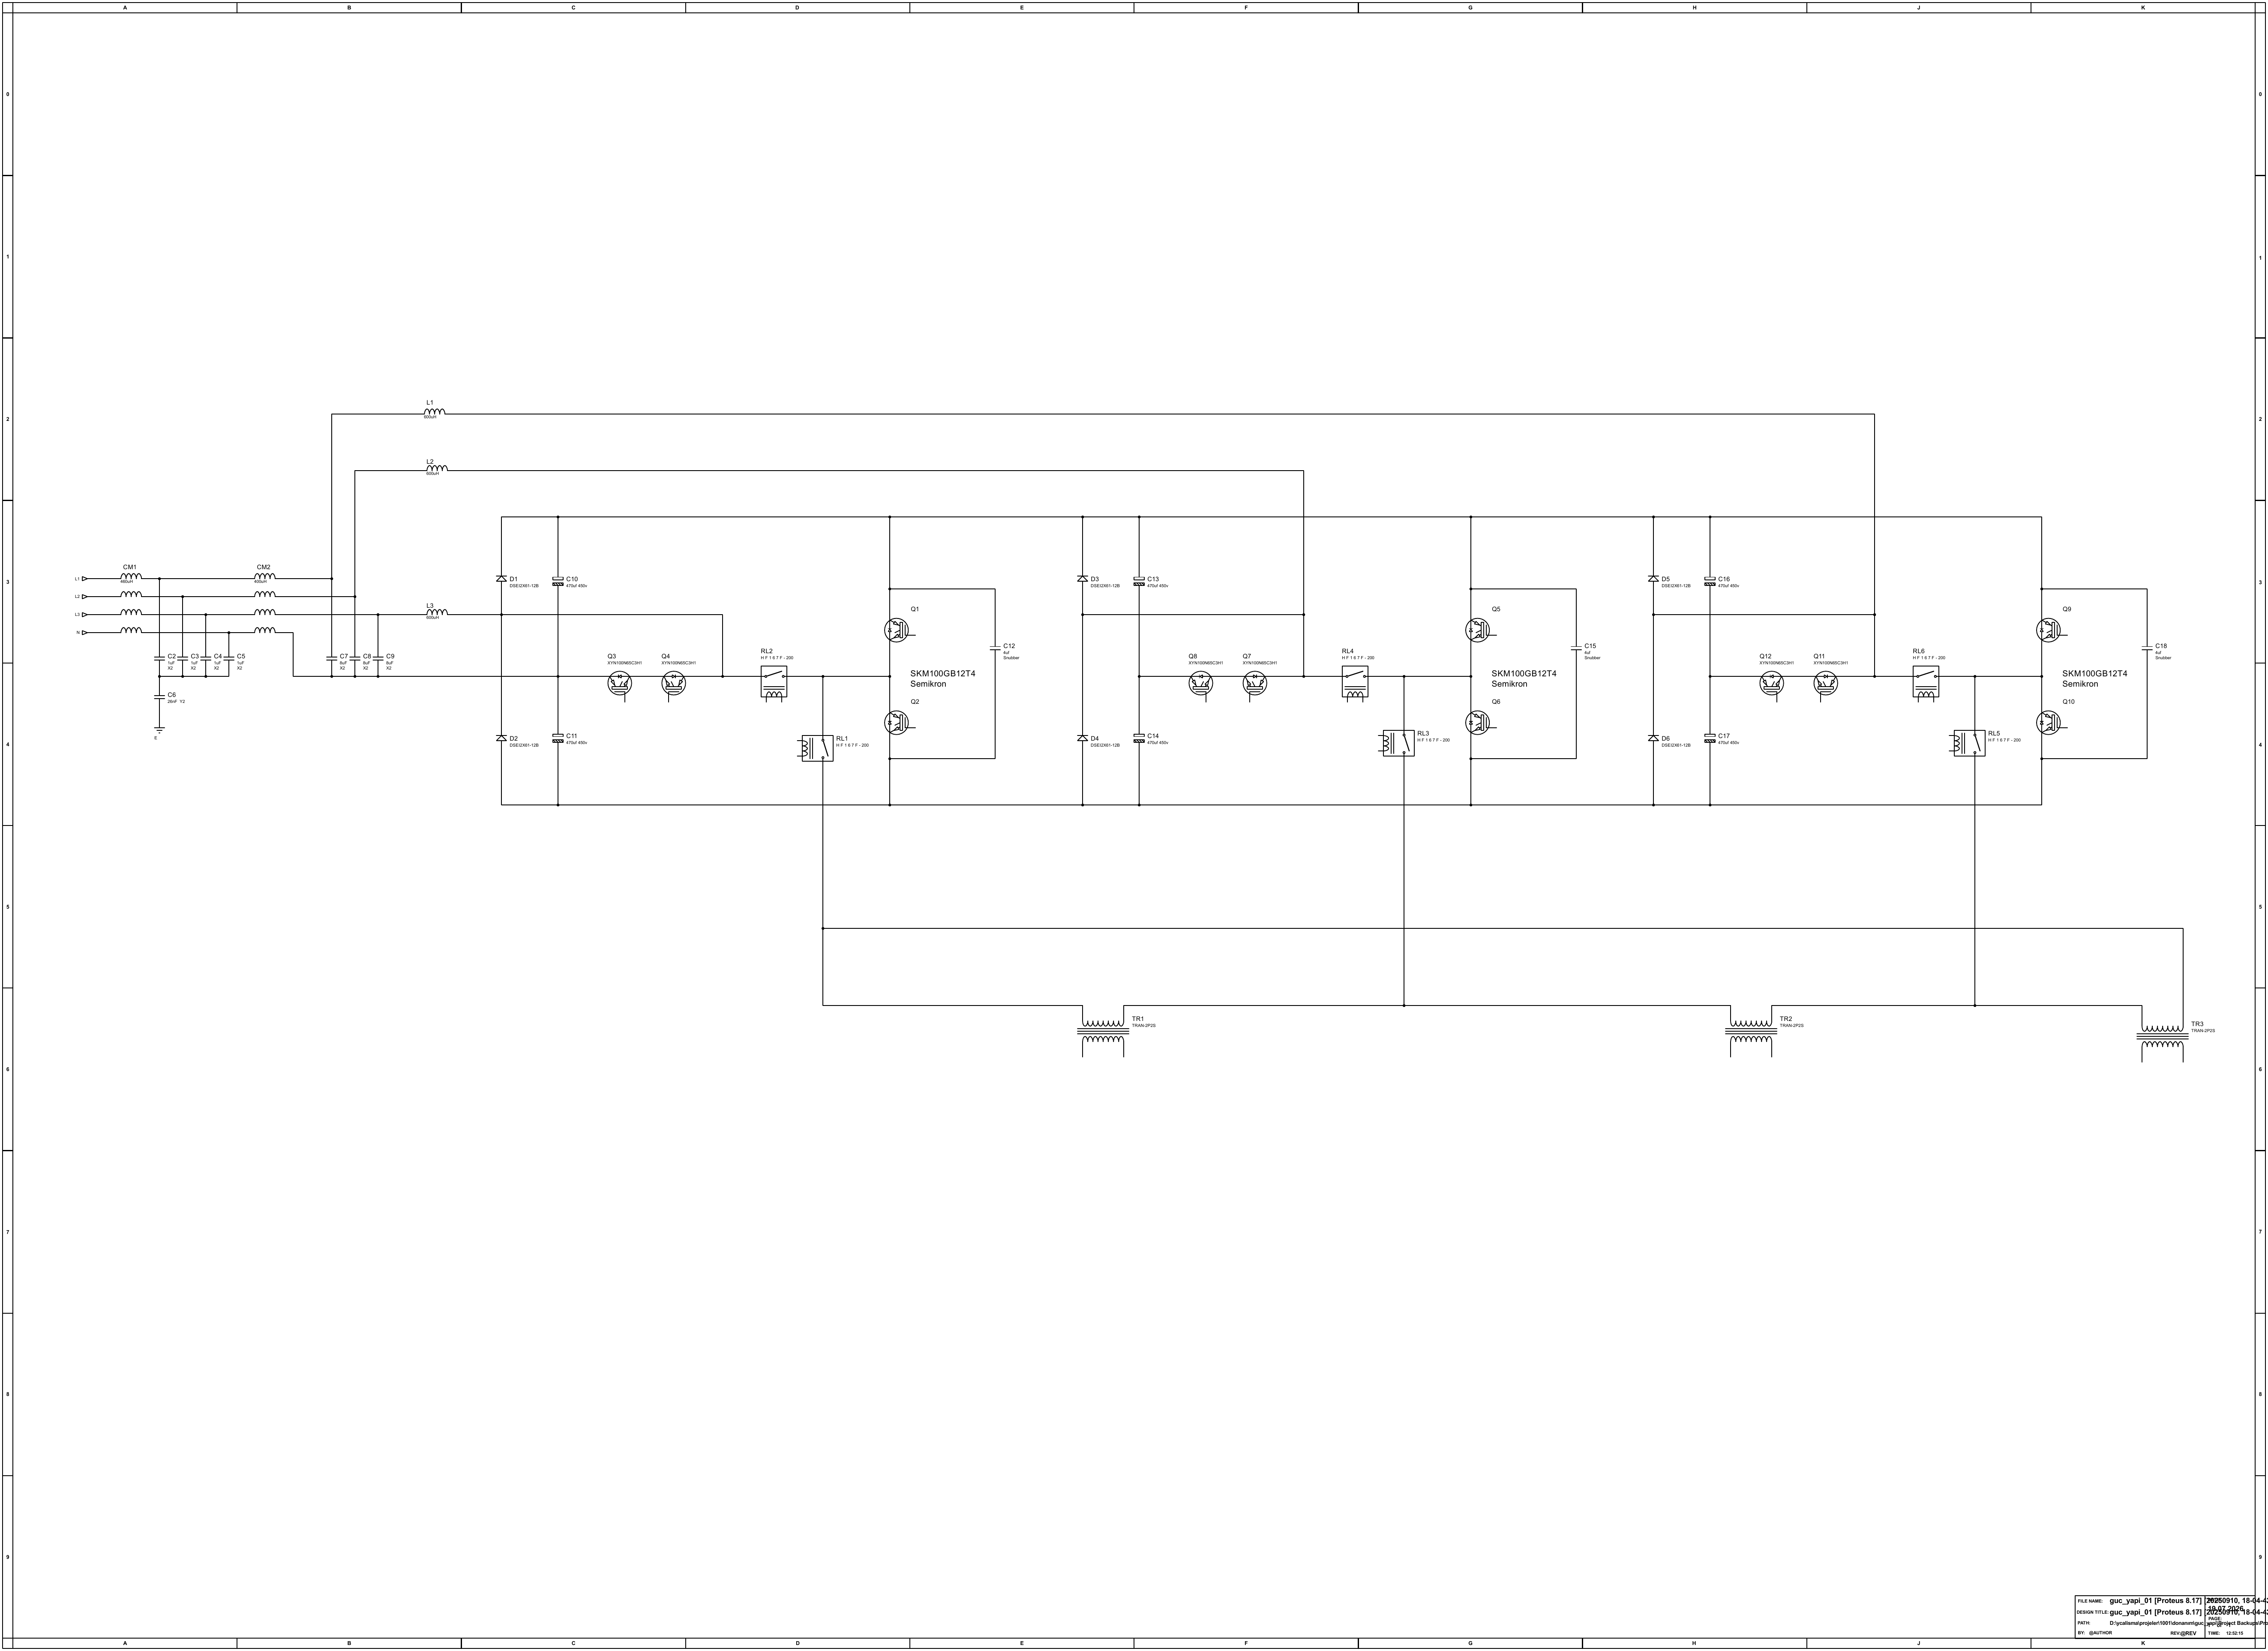
\includegraphics[width=\textwidth]{sistem/tam_topoloji_20260822.png}
  \caption{Üç fazlı tam güç topolojisi: ortak giriş/EMI ağı, üç tekrarlı T-tipi faz hücresi, akım algılama--röle yolları ve gerilim algılama transformatörleri. Şema, yöntem bölümünde sistem sınırı ve faz-başına indirgeme kaynağı olarak kullanılmıştır.}
  \label{fig:gelen-tam-topoloji}
\end{figure}

Faz indisi $x\in\{a,b,c\}$, DA bara orta noktası $N$, faz kutup gerilimi $v_{xN}$ ve gerilim durumunu seçen boyutsuz anahtarlama değişkeni $s_x\in\{-1,0,1\}$ ile gösterilsin. Üç gerilim durumu
\begin{equation}
  v_{xN}=s_x\frac{V_{\mathrm{dc}}}{2}
  \label{eq:t-tipi-anahtarlama-fonksiyonu}
\end{equation}
biçiminde ortak bir gösterime indirgenebilir. Eşitlik~\eqref{eq:t-tipi-anahtarlama-fonksiyonu}, $s_x=1$, $0$ ve $-1$ için sırasıyla pozitif, sıfır ve negatif kutup gerilimini verir. Doğrusal modülasyon bölgesinde normalize faz komutu $m_x=2v_x^{\ast}/V_{\mathrm{dc}}$ olmak üzere pozitif, negatif ve sıfır durumlarının boyutsuz ideal görev oranları $d_P$, $d_N$ ve $d_O$
\begin{equation}
  d_P=\max(m_x,0),\qquad
  d_N=\max(-m_x,0),\qquad
  d_O=1-|m_x|,\qquad |m_x|\leq 1
  \label{eq:t-tipi-gorev-oranlari}
\end{equation}
olarak yazılabilir \citep{Holmes2003,Wang2020}. Eşitlik~\eqref{eq:t-tipi-gorev-oranlari}, modülasyon komutunun genliği azaldığında sıfır durumunun payının neden arttığını doğrudan göstermektedir. Gerçek taşıyıcı tabanlı PWM'de örnekleme, minimum darbe, ölü zaman ve nötr nokta dengeleme müdahaleleri ideal görev oranlarını değiştirebilir; söz konusu etkiler kapı kodu doğrulamasında ayrıca ele alınacaktır.

Üç gerilim seviyesinin devre karşılığı Şekil~\ref{fig:t-tipi-uc-seviye} üzerinde tek karşılaştırmalı görünüm altında verilmiştir. Aynı devre tabanının korunması, hangi anahtarlama durumunun yalnızca bağlantı noktasını değiştirdiğini görmeyi kolaylaştırmaktadır.

\begin{figure}[htbp]
  \centering
  \begin{subfigure}[t]{0.32\textwidth}
    \centering
    \resizebox{\linewidth}{!}{\ttypevector{green!55!black}{gray!65}{gray!65}{gray!65}{%
      \draw[activepath] (4,5) -- (q1.north);
      \draw[activepath] (q1.south) -- (out) -- (5.0,2);}}
    \caption{$P$: $+V_{\mathrm{dc}}/2$}
  \end{subfigure}\hfill
  \begin{subfigure}[t]{0.32\textwidth}
    \centering
    \resizebox{\linewidth}{!}{\ttypevector{gray!65}{gray!65}{green!55!black}{green!55!black}{%
      \draw[activepath] (0,2) -- (q3.west);
      \draw[activepath] (q3.east) -- (q4.west);
      \draw[activepath] (q4.east) -- (out) -- (5.0,2);}}
    \caption{$O$: $0$}
  \end{subfigure}\hfill
  \begin{subfigure}[t]{0.32\textwidth}
    \centering
    \resizebox{\linewidth}{!}{\ttypevector{gray!65}{green!55!black}{gray!65}{gray!65}{%
      \draw[activepath] (4,-1) -- (q2.south);
      \draw[activepath] (q2.north) -- (out) -- (5.0,2);}}
    \caption{$N$: $-V_{\mathrm{dc}}/2$}
  \end{subfigure}
  \caption{T-tipi faz kolunun üç gerilim durumu. Yeşil anahtarlar ve mavi bağlantılar ilgili durumun etkin elemanlarını göstermektedir.}
  \label{fig:t-tipi-uc-seviye}
\end{figure}

Tablo~\ref{tab:t-tipi-durumlar}, kapı durumlarını literatürdeki üç seviyeli gösterimle birlikte özetlemektedir \citep{Holmes2003,Wang2020}. ``1'' iletim komutunu, ``0'' kesim komutunu ifade etmektedir. Tablo yalnızca ideal kararlı durumları göstermekte; ölü zaman sırasında diyot iletimi ve akım yönüne bağlı geçici komütasyon yolları kapsam dışı bırakılmaktadır.

\begin{table}[htbp]
  \centering
  \caption{T-tipi faz kolunun ideal anahtarlama durumları ve kapı komutları.}
  \label{tab:t-tipi-durumlar}
  \small
  \begin{tabularx}{\textwidth}{c c c c c c X}
    \toprule
    Durum & $Q_1$ & $Q_2$ & $Q_3$ & $Q_4$ & $v_{xN}$ & İşlevsel açıklama \\
    \midrule
    $P$ & 1 & 0 & 1 & 0 & $+V_{\mathrm{dc}}/2$ & Pozitif yarım periyotta enerji üst DA bara kolundan faz çıkışına aktarılır. \\
    $O$ & 0 & 0 & 1 & 1 & $0$ & Faz çıkışı nötr kola bağlanır; filtre akımının yönüne göre serbest dolaşım yolu oluşur. \\
    $N$ & 0 & 1 & 0 & 1 & $-V_{\mathrm{dc}}/2$ & Negatif yarım periyotta enerji alt DA bara kolu üzerinden aktarılır. \\
    \bottomrule
  \end{tabularx}
\end{table}

$P$ durumunda $Q_3$ ve $N$ durumunda $Q_4$ için verilen iletim komutu, yarım periyot etkinleştirme kuralını yansıtmaktadır; ilgili nötr anahtar aktif enerji yolunda akım taşımamaktadır. Yalnızca gerilim seviyesini üreten asgari durum gösterilecekse $P$ için $Q_1$, $O$ için $Q_3$--$Q_4$ ve $N$ için $Q_2$ iletimde kabul edilebilir. Nihai kapı tablosu, gerçek PWM kodundaki komut dizisiyle karşılaştırılarak bu iki gösterimden hangisinin kullanıldığı açıkça belirtilecektir.

Pozitif yarım periyotta modülasyon, $P$ ve $O$ durumları arasında; negatif yarım periyotta ise $N$ ve $O$ durumları arasında yapılır. Endüktif çıkış filtresi nedeniyle faz akımı anahtarlama anında sürekliliğini korur. Gerilim komutu değişse bile akımın mevcut yönü, aktif anahtarın kanalı veya antiparalel diyot üzerinden uygun serbest dolaşım yolunu belirler. Yalnızca kapı komutlarına bakmak bu yüzden gerçek iletimde bulunan yarı iletkeni tanımlamak için yeterli değildir.

Şekil~\ref{fig:t-tipi-akim-yollari}(a), $C_A$--$C_B$ bölünmüş DA barayı, antiparalel diyotlu $Q_1$--$Q_4$ IGBT'lerini ve faz başına $L_1$--$C_f$--$L_2$ filtresini tek topolojide birleştirmektedir. Şekil~\ref{fig:t-tipi-akim-yollari}(b)--(e), aynı güç katının dört temel iletim yolunu karşılaştırmaktadır; akım yolu okunabilirliğini korumak için filtre elemanları alt çizimlerde tekrarlanmamıştır. Pozitif alternansın aktif durumunda $Q_1$ üzerinden, sıfır durumunda nötr kol üzerinden akış gerçekleşir. Negatif alternansta aynı işleyiş alt kol için simetrik biçimde oluşur. Nötr seviyesinde geçirilen sürenin modülasyon indeksi azaldıkça artması, düşük güçte nötr anahtarların iletim payını ve ters akım riskini büyütmektedir.

\begin{figure}[htbp]
  \centering
  \begin{subfigure}[t]{0.96\textwidth}
    \centering
    \resizebox{0.98\linewidth}{!}{\ttypefulltopology}
    \caption{Faz başına tam güç topolojisi ve LCL filtre}
  \end{subfigure}

  \vspace{4mm}
  \begin{subfigure}[t]{0.48\textwidth}
    \centering
    \ttypevector{green!55!black}{gray!65}{gray!65}{gray!65}{%
      \draw[current] (0.7,5) -- (q1.north);
      \draw[current] (q1.south) -- (out) -- (5.0,2);}
    \caption{Pozitif alternans, aktif $P$ durumu}
  \end{subfigure}\hfill
  \begin{subfigure}[t]{0.48\textwidth}
    \centering
    \ttypevector{gray!65}{gray!65}{green!55!black}{green!55!black}{%
      \draw[current] (0.5,2) -- (q3.west);
      \draw[current] (q3.east) -- (q4.west);
      \draw[current] (q4.east) -- (5.0,2);}
    \caption{Pozitif alternans, sıfır $O$ durumu}
  \end{subfigure}

  \vspace{4mm}
  \begin{subfigure}[t]{0.48\textwidth}
    \centering
    \ttypevector{gray!65}{green!55!black}{gray!65}{gray!65}{%
      \draw[current] (5.0,2) -- (out) -- (q2.north);
      \draw[current] (q2.south) -- (0.7,-1);}
    \caption{Negatif alternans, aktif $N$ durumu}
  \end{subfigure}\hfill
  \begin{subfigure}[t]{0.48\textwidth}
    \centering
    \ttypevector{gray!65}{gray!65}{green!55!black}{green!55!black}{%
      \draw[current] (5.0,2) -- (q4.east);
      \draw[current] (q4.west) -- (q3.east);
      \draw[current] (q3.west) -- (0.5,2);}
    \caption{Negatif alternans, sıfır $O$ durumu}
  \end{subfigure}
  \caption{T-tipi faz kolunun devre yapısı ve dört temel akım yolunun ortak devre dili ve renk lejandıyla vektörel gösterimi. Tam topoloji $C_A$, $C_B$, antiparalel diyotlu IGBT'ler, $L_1$, $C_f$ ve $L_2$ elemanlarını; kırmızı oklar ise tanımlanan pozitif akım yönüne göre iletim yollarını göstermektedir.}
  \label{fig:t-tipi-akim-yollari}
\end{figure}

\begin{samepage}
  Şekil~\ref{fig:t-tipi-akim-yollari}(a), faz kolunun işlevsel güç topolojisidir; kart üretim veya bağlantı şeması niteliği taşımamaktadır. Kapı sürücüleri, sensörler, koruma devreleri, konektörler, yarı iletken parça kodları ve kesin pasif eleman değerlerini içeren ayrıntılı uygulama şeması, gerçek donanım kaydıyla doğrulandıktan sonra Ek~A'da verilecektir.
\end{samepage}

\section{Düşük Güç Eşdeğeri ve Ters Akım Mekanizması}

Faz gerilimi referansının genliği azaldığında aktif $P$ veya $N$ durumunun görev oranı küçülür, sıfır durumunun süresi uzar. Pozitif ve negatif yarım periyotlar ayrı ayrı ele alındığında faz kolu, anahtarlanan gerilim kaynağı ile filtre endüktansı bakımından senkron alçaltıcı dönüştürücüye eşdeğer bir davranış gösterir \citep{Mohan2003,Erickson2001}. İki yarım periyodun eşdeğerleri Şekil~\ref{fig:senkron-buck-esdeger} altında bir araya getirilmiştir.

\begin{figure}[htbp]
  \centering
  \begin{subfigure}[t]{0.46\textwidth}
    \centering
    \resizebox{\linewidth}{!}{\syncbuckvector{$+V_{\mathrm{dc}}/2$}{$N$}{$Q_1$}{$Q_3$}}
    \caption{Pozitif yarım periyot eşdeğeri}
  \end{subfigure}\hfill
  \begin{subfigure}[t]{0.46\textwidth}
    \centering
    \resizebox{\linewidth}{!}{\syncbuckvector{$N$}{$-V_{\mathrm{dc}}/2$}{$Q_4$}{$Q_2$}}
    \caption{Negatif yarım periyot eşdeğeri}
  \end{subfigure}
  \caption{T-tipi faz kolunun yarım periyotlara göre senkron-buck eşdeğerleri. Yeşil anahtar ve mavi yol aktif enerji aktarımını göstermektedir.}
  \label{fig:senkron-buck-esdeger}
\end{figure}

Anahtarlama periyodu $T_{\mathrm{s}}$, boyutsuz görev oranı $d\in[0,1]$, faz koluna uygulanan etkin DA gerilimi $V_{\mathrm{h}}$, anık şebeke gerilimi $v_{\mathrm{g}}$, eşdeğer filtre endüktansı $L$ ve anahtarın iletim/kesim aralıklarındaki endüktör gerilimleri $v_{L,\mathrm{on}}$ ile $v_{L,\mathrm{off}}$ olarak tanımlansın. Pozitif yarım periyotta ideal gerilimler
\begin{equation}
  \begin{aligned}
    v_{L,\mathrm{on}} &= V_{\mathrm{h}}-v_{\mathrm{g}}, \\
    v_{L,\mathrm{off}} &= -v_{\mathrm{g}}
  \end{aligned}
  \label{eq:buck-enduktor-gerilimleri}
\end{equation}
biçimindedir. Eşitlik~\eqref{eq:buck-enduktor-gerilimleri} altında anahtarlama periyodu boyunca gerilimlerin yaklaşık sabit kaldığı ve yerel kararlı durumda volt--saniye dengesinin sağlandığı kabul edilirse tepe--tepe akım dalgalanması $\Delta i_L$
\begin{equation}
  \Delta i_L \simeq \frac{(V_{\mathrm{h}}-v_{\mathrm{g}})dT_{\mathrm{s}}}{L}
  =\frac{v_{\mathrm{g}}(1-d)T_{\mathrm{s}}}{L}
  \label{eq:buck-akim-dalgalanmasi}
\end{equation}
ile bulunur \citep{Erickson2001,Chen2010}. Eşitlik~\eqref{eq:buck-akim-dalgalanmasi} içindeki iki ifade yalnızca aynı yerel volt--saniye dengesi altında eşdeğerdir. Ortalama akım $\bar{i}_L$ değerinin dalgalanmanın yarısından küçük olduğu bölgede akım sıfırı geçebilir:
\begin{equation}
  \bar{i}_L < \frac{\Delta i_L}{2}.
  \label{eq:ters-akim-esigi}
\end{equation}
Senkron anahtar sıfır geçişinden sonra iletimde tutulursa $i_L<0$ aralığı oluşur ve filtredeki enerji DA tarafa geri taşınır. Yararlı çıkış gücüne katkı sağlamayan söz konusu dolaşım, RMS akımı ile iletim kayıplarını artırabilir. Diyot benzetimi yaklaşımı, akım sıfıra yaklaştığında senkron yolu keserek negatif akımı engeller; sıfır akım algılamadaki gecikme ve anahtarlama geçişleri ise gerçek kayıp sınırını belirler \citep{Chen2010,Erickson2001}. Diyot benzetimi ile sürekli iletim arasındaki temel fark, Bölüm~\ref{chap:literatur} içindeki Şekil~\ref{fig:de-ccm-akim} üzerinde birincil kaynakla gösterilmiştir; mevcut bölüm aynı genel davranışı Eşitlik~\eqref{eq:ters-akim-esigi} ile T-tipi faz koluna uyarlamaktadır.

T-tipi faz kolunda nötr anahtarların susturulması benzer bir amaç taşımaktadır: düşük güçte, referans akım yönüne ters enerji dolaşımı oluşturan komütasyonların azaltılması hedeflenir. Yaklaşım, klasik PWM'nin bütün çalışma aralığında değiştirilmesi yerine belirlenen düşük güç veya küçük modülasyon bölgesinde etkinleştirilmelidir. Eşik seçimi yalnızca akım genliğine bağlanamaz; akım dalgalanması, ölçüm gürültüsü, ölü zaman, şebeke gerilimi ve hesaplama gecikmesi de karar mantığına dâhil edilmelidir.

\section{LCL Filtre ve Şebeke Modeli}

Şebeke bağlantılı eviricide LCL filtre, anahtarlama frekansı çevresindeki gerilim bileşenlerini daha küçük toplam endüktansla bastırabilmektedir. Rezonans tepesi ve şebeke empedansına duyarlılık, filtreyi yalnızca pasif bir zayıflatıcı olmaktan çıkarıp kapalı çevrim tasarımının parçası hâline getirir \citep{Zhang2014PR,Lu2016}. Faz başına ortalama modelde evirici tarafı endüktansı $L_1$, filtre kapasitörü $C_f$, şebeke tarafı endüktansı $L_2$, seri kayıplar $R_1$ ve $R_2$ ile gösterilmiştir. Şebeke eşdeğer endüktansı gerektiğinde $L_2$ içine eklenmektedir.

Şekil~\ref{fig:faz-basina-lcl-modeli}, durum denklemlerinde kullanılan işaretleri fiziksel ölçüm noktalarıyla eşleştirmektedir. $i_1$ evirici tarafı endüktör akımını, $i_2$ ortak bağlantı noktasına aktarılan şebeke akımını ve $v_c$ filtre kapasitörü gerilimini göstermektedir. Gerçek donanımda ölçülen akımın $i_1$ veya $i_2$ olması, denetleyici bitki modelini ve aktif sönümleme yolunu değiştireceğinden sensör konumu kod ve devre şemasıyla kesinleştirilecektir.

\begin{figure}[htbp]
  \centering
  \resizebox{0.96\textwidth}{!}{%
  \begin{tikzpicture}[
    block/.style={draw,rounded corners=1pt,minimum width=13mm,minimum height=8mm,fill=blue!4},
    resistor/.style={draw,minimum width=8mm,minimum height=5mm,fill=white},
    coilpath/.style={decorate,decoration={coil,aspect=0.48,segment length=2.9mm,amplitude=1.9mm}},
    sensor/.style={circle,draw,fill=orange!10,minimum size=7mm,font=\scriptsize},
    flow/.style={-{Latex[length=2mm]},line width=1.0pt},
    current/.style={-{Latex[length=2mm]},red!80!black,line width=1.0pt},
    wire/.style={line width=0.9pt},
    signal/.style={-{Latex[length=1.8mm]},dashed,gray!80}
  ]
    \node[block,align=center] (inv) at (0,0) {T-tipi\\faz kolu};
    \node[resistor] (r1) at (1.65,0) {$R_1$};
    \coordinate (l1a) at (2.35,0);
    \coordinate (l1b) at (3.45,0);
    \coordinate (vc) at (4.10,0);
    \node[resistor] (r2) at (5.30,0) {$R_2$};
    \coordinate (l2a) at (5.95,0);
    \coordinate (l2b) at (7.05,0);
    \node[block,align=center] (grid) at (8.55,0) {Şebeke\\$v_g$};
    \draw[wire] (inv.east) -- node[above,font=\scriptsize] {$v_{\mathrm{inv}}$} (r1.west);
    \draw[wire] (r1.east) -- (l1a);
    \draw[coilpath,line width=0.9pt] (l1a) -- (l1b);
    \draw[wire] (l1b) -- (vc) -- (r2.west);
    \draw[wire] (r2.east) -- (l2a);
    \draw[coilpath,line width=0.9pt] (l2a) -- (l2b);
    \draw[wire] (l2b) -- (grid.west);
    \node[above=2mm,font=\scriptsize] at ($(l1a)!0.5!(l1b)$) {$L_1$};
    \node[above=2mm,font=\scriptsize] at ($(l2a)!0.5!(l2b)$) {$L_2$};
    \draw[current] (2.30,0.55) -- node[above,font=\scriptsize] {$i_1$} (3.45,0.55);
    \draw[current] (5.90,0.55) -- node[above,font=\scriptsize] {$i_2$} (7.05,0.55);
    \fill (vc) circle (1.6pt);
    \draw[line width=0.8pt] (vc) -- (4.10,-0.8);
    \draw[line width=0.8pt] (3.73,-0.8) -- (4.47,-0.8);
    \draw[line width=0.8pt] (3.73,-1.08) -- (4.47,-1.08);
    \draw[line width=0.8pt] (4.10,-1.08) -- (4.10,-1.50);
    \draw[line width=0.8pt] (3.73,-1.50) -- (4.47,-1.50);
    \draw[line width=0.8pt] (3.83,-1.65) -- (4.37,-1.65);
    \draw[line width=0.8pt] (3.95,-1.80) -- (4.25,-1.80);
    \node[right,font=\scriptsize] at (4.40,-0.94) {$C_f$};
    \node[above,font=\scriptsize] at (vc) {$v_c$};
    \node[sensor] (si1) at (2.90,-2.25) {$i_1$};
    \node[sensor] (svc) at (4.10,-2.25) {$v_c$};
    \node[sensor] (si2) at (6.50,-2.25) {$i_2$};
    \node[block,fill=gray!8,align=center] (adc) at (4.85,-3.55) {Ölçüm ve\\ADC zinciri};
    \draw[signal] ($(l1a)!0.5!(l1b)$) -- (si1.north);
    \draw[signal] (vc) -- (svc.north);
    \draw[signal] ($(l2a)!0.5!(l2b)$) -- (si2.north);
    \draw[signal] (si1) -- (adc);
    \draw[signal] (svc) -- (adc);
    \draw[signal] (si2) -- (adc);
  \end{tikzpicture}%
  }
  \caption{Faz başına LCL filtre, durum değişkenleri ve denetimde kullanılacak aday ölçüm noktaları.}
  \label{fig:faz-basina-lcl-modeli}
\end{figure}

Evirici kutup gerilimi $v_{\mathrm{inv}}$, kapasitör gerilimi $v_c$, şebeke gerilimi $v_g$, evirici tarafı akımı $i_1$ ve şebeke akımı $i_2$ için durum denklemleri
\begin{equation}
  \begin{aligned}
    L_1\frac{\mathrm{d}i_1}{\mathrm{d}t} &= v_{\mathrm{inv}}-v_c-R_1i_1, \\
    C_f\frac{\mathrm{d}v_c}{\mathrm{d}t} &= i_1-i_2, \\
    L_2\frac{\mathrm{d}i_2}{\mathrm{d}t} &= v_c-v_g-R_2i_2
  \end{aligned}
  \label{eq:lcl-durum-denklemleri}
\end{equation}
olarak elde edilir. Eşitlik~\eqref{eq:lcl-durum-denklemleri} içindeki $L_1$, $L_2$ ve $C_f$ enerji depolayan filtre elemanlarını; $R_1$ ile $R_2$ seri eşdeğer kayıpları temsil eder. Laplace değişkeni $s$, $i_2(t)$ ve $v_{\mathrm{inv}}(t)$ işaretlerinin Laplace dönüşümleri sırasıyla $I_2(s)$ ve $V_{\mathrm{inv}}(s)$ olarak tanımlansın. Kayıpların ihmal edildiği modelde $v_g=0$ alınarak modülasyon geriliminden şebeke akımına aktarım
\begin{equation}
  G_{vi}(s)=\frac{I_2(s)}{V_{\mathrm{inv}}(s)}
  =\frac{1}{L_1L_2C_fs^3+(L_1+L_2)s}
  \label{eq:lcl-aktarim}
\end{equation}
şeklindedir. Eşitlik~\eqref{eq:lcl-aktarim} kayıpsız ve şebeke gerilimi bozucusu sıfırlanmış ideal bitkiyi tanımlar. Rezonans açısal frekansı $\omega_r$ ve hertz cinsinden rezonans frekansı $f_r$
\begin{equation}
  \omega_r=\sqrt{\frac{L_1+L_2}{L_1L_2C_f}},
  \qquad f_r=\frac{\omega_r}{2\pi}
  \label{eq:lcl-rezonans}
\end{equation}
ile hesaplanır. Eşitlik~\eqref{eq:lcl-rezonans}, seri kayıpları ve ek sönümleme kolunu içermeyen ideal LCL sonucudur. Gerçek modelde seri dirençler, kapasitör sönümleme kolu, sayısal gecikme ve şebeke empedansı aktarım fonksiyonuna eklenmelidir. Kararlılık incelemesinde kullanılan $L(s)$, $S(s)$ ve $T(s)$ fonksiyonları bu fiziksel model üzerinden Bölüm~\ref{chap:sin3} içinde üretilecek; yalnızca ideal LCL ifadesinden çizilen Bode grafiği nihai kanıt sayılmayacaktır.

\section{Denetim, Modülasyon ve Sin\texorpdfstring{\textsuperscript{3}}{3} Kompanzasyonu}

Akım döngüsü, referans akım $i^{\ast}$ ile ölçülen şebeke veya evirici tarafı akımı arasındaki hatadan modülasyon komutu üretir. PR denetleyicisinin aktarımı $C_i(s)$, oransal kazanç $K_p$, rezonans kazanç $K_r$, şebeke temel açısal frekansı $\omega_0$ ve pratik rezonans bandını belirleyen pozitif bant katsayısı $\omega_c$ ile gösterilsin. Sinüzoidal referansın kalıcı durum hatasını azaltmak için kullanılabilecek genel yapı
\begin{equation}
  C_i(s)=K_p+\frac{2K_r\omega_c s}{s^2+2\omega_c s+\omega_0^2}
  \label{eq:pr-denetleyici}
\end{equation}
biçiminde gösterilebilir \citep{Teodorescu2006PR,Zhang2014PR}. Eşitlik~\eqref{eq:pr-denetleyici} içindeki $\omega_c$, ideal sonsuz kazançlı rezonatör yerine sonlu bantlı uygulama modelini verir. Kullanılan gerçek denetleyici yapısı, yazılım kodu ve parametre kayıtlarıyla doğrulandıktan sonra denklem ve parametre tablosunda kesinleştirilecektir.

Referans ve ölçülen akımların Laplace dönüşümleri $I^{\ast}(s)$ ile $I(s)$; normalize toplam modülasyon komutu, klasik ileri besleme ve Sin\textsuperscript{3} yolu sırasıyla $U_{\mathrm{mod}}^{\ast}(s)$, $U_{\mathrm{ff}}(s)$ ve $U_{\sin^3}(s)$ olarak tanımlansın. Modülasyon komutu kavramsal olarak
\begin{equation}
  U_{\mathrm{mod}}^{\ast}(s)=C_i(s)\left[I^{\ast}(s)-I(s)\right]+U_{\mathrm{ff}}(s)+U_{\sin^3}(s)
  \label{eq:modulasyon-toplami}
\end{equation}
şeklinde ayrılmıştır. Eşitlik~\eqref{eq:modulasyon-toplami} zaman alanı işaretleriyle aktarım fonksiyonunu aynı ifadede karıştırmamak için tamamen Laplace alanında yazılmıştır. $U_{\mathrm{ff}}$ şebeke gerilimi veya bozucu bastırma amacıyla kullanılan klasik ileri besleme terimini, $U_{\sin^3}$ ise önerilen ikincil şekillendirmeyi temsil eder. PLL faz açısı $\theta$ için trigonometrik özdeşlik
\begin{equation}
  \sin^3(\theta)=\frac{3\sin(\theta)-\sin(3\theta)}{4}
  \label{eq:sin3-ozdeslik}
\end{equation}
kompanzasyonun temel ve üçüncü harmonik bileşenlerini açıkça göstermektedir. Eşitlik~\eqref{eq:sin3-ozdeslik} içindeki $\theta$ boyutsuz elektriksel açıdır. Katsayı ve işaret, gözlenen üçüncü harmonik bozulumunu azaltacak biçimde belirlenmeli; terim doygunluk ve modülasyon sınırlarından önce uygun sınırlayıcılarla uygulanmalıdır.

Ölçümden kapı işaretine uzanan işlevsel zincir Şekil~\ref{fig:denetim-modulasyon-blok} üzerinde izlenebilir bir blok yapısına dönüştürülmüştür. Yapı, Sin\textsuperscript{3} yolunun akım denetleyicisiyle seri değil modülasyon toplamında paralel bir ileri besleme bileşeni olduğunu ve nötr anahtar susturma kararının PWM üretiminden sonra kapı mantığında uygulandığını açıkça ayırmaktadır.

\begin{figure}[H]
  \centering
  \resizebox{0.99\textwidth}{!}{%
  \begin{tikzpicture}[
    node distance=5mm and 5mm,
    block/.style={draw,rounded corners=1.3pt,align=center,minimum height=9mm,minimum width=14mm,fill=blue!5},
    special/.style={draw,rounded corners=1.3pt,align=center,minimum height=9mm,minimum width=18mm,fill=orange!12},
    sum/.style={circle,draw,minimum size=7mm,inner sep=0pt},
    flow/.style={-{Latex[length=1.8mm]},line width=0.9pt},
    feedback/.style={-{Latex[length=1.8mm]},line width=0.9pt,dashed}
  ]
    \node[block] (iref) {$i^{\ast}$\\üretimi};
    \node[sum,right=of iref] (sumi) {$\Sigma$};
    \node[block,right=of sumi] (ci) {$C_i(s)$\\akım denetimi};
    \node[sum,right=of ci] (sumv) {$\Sigma$};
    \node[block,right=of sumv,minimum width=24mm] (pwm) {Sınırlandırma, ölçekleme\\ve PWM üretimi};
    \node[special,right=of pwm,minimum width=25mm] (gate) {$Q_1$--$Q_4$ kapı mantığı\\ve nötr susturma};
    \node[block,right=of gate,minimum width=20mm] (plant) {T-tipi güç katı\\ve LCL filtre};
    \draw[flow] (iref) -- (sumi);
    \draw[flow] (sumi) -- node[above,font=\scriptsize] {$e_i$} (ci);
    \draw[flow] (ci) -- (sumv);
    \draw[flow] (sumv) -- node[above,font=\scriptsize] {$v_{\mathrm{mod}}^{\ast}$} (pwm);
    \draw[flow] (pwm) -- (gate);
    \draw[flow] (gate) -- node[above,font=\scriptsize] {$q_1$--$q_4$} (plant);

    \node[special,below=13mm of ci,xshift=-7mm,text width=23mm] (vff) {Şebeke gerilimi\\ileri besleme $v_{\mathrm{ff}}$};
    \node[special,below=13mm of sumv,xshift=11mm,minimum width=20mm] (sin3) {Sin\textsuperscript{3}\\$K_{\sin^3}\sin^3\theta$};
    \node[block,below=11mm of iref] (pll) {Faz bilgisi\\$\theta$};
    \node[block,below=11mm of plant] (meas) {Ölçüm, ADC\\ve ölçekleme};
    \draw[flow] (pll) -- (iref);
    \coordinate (phasebus) at ($(pll.south)+(0,-0.65)$);
    \draw[flow] (pll.south) -- (phasebus) -| (sin3.south);
    \draw[flow] (vff) -| (sumv.south);
    \draw[flow] (sin3) -- (sumv.south);
    \draw[feedback] (plant.south) -- (meas.north);
    \coordinate (feedbackbus) at ($(vff.south)+(0,-1.0)$);
    \draw[feedback] (meas.south) |- (feedbackbus) -| node[pos=0.72,below,font=\scriptsize] {$i_{\mathrm{ölç}}$} (sumi.south);
    \node[font=\scriptsize] at ($(sumi)+(-0.24,0.34)$) {$+$};
    \node[font=\scriptsize] at ($(sumi)+(-0.24,-0.34)$) {$-$};
    \node[font=\scriptsize] at ($(sumv)+(-0.24,0.34)$) {$+$};
    \pgfresetboundingbox
    \coordinate (bboxse) at (meas.east |- feedbackbus);
    \path[use as bounding box] ($(iref.north west)+(-0.3,0.35)$) rectangle ($(bboxse)+(0.3,-0.3)$);
  \end{tikzpicture}%
  }
  \caption{İşlevsel akım denetimi, ileri besleme, Sin\textsuperscript{3}, PWM ve nötr anahtar susturma blokları.}
  \label{fig:denetim-modulasyon-blok}
\end{figure}

İdeal doğrusal modelde dışsal ileri besleme terimi karakteristik paydayı değiştirmeyebilir. Sayısal uygulamada örnekleme, sıfırıncı derece tutucu, PWM, hesaplama ve ölçüm filtreleri toplam bir gecikme $G_d(s)$ oluşturur. Şekil~\ref{fig:denetim-modulasyon-blok} içindeki küçük harfli $v_{\mathrm{ff}}(t)$, $v_{\sin^3}(t)$ ve $v_{\mathrm{mod}}^{\ast}(t)$ zaman alanındaki fiziksel/normalize komutları; Eşitlik~\eqref{eq:modulasyon-toplami} içindeki büyük harfler aynı işaretlerin Laplace dönüşümlerini gösterir. Şebeke gerilimi ileri beslemesinin LCL rezonansında pozitif veya negatif sönümleme üretmesi mümkün olduğundan iki ileri besleme yolu kapalı çevrim analizinde ayrı girişler olarak tutulacaktır \citep{Lu2016,Wang2024}. Sin\textsuperscript{3} teriminin başarısı bu yüzden yalnızca düşük güç THD değeriyle değil; akım izleme hatası, kararlılık marjı, kontrol eforu, doyum süresi ve anma gücündeki etkisizliği veya güvenli katkısı ile birlikte değerlendirilecektir.

\eksikistek{Gerçek denetim kodu ve kapı mantığı}{Şekil~\ref{fig:denetim-modulasyon-blok} yöntem düzeyinde tamamlanmıştır; denetleyici türü, işaret yönleri, sınırlayıcı sırası, PWM güncelleme anı, kapı eşlemesi ve nötr susturma koşulunun bire bir doğrulanması için gerçek PWM/denetleyici kaynak kodunu istiyoruz (istek listesi R05--R06). Ayrıca Senaryo~2--4'e ait model veya kod paketleri istiyoruz; eldeki tek kaynak model Senaryo~1'e aittir ve R2025b'de kaldırılan ölçüm blokları nedeniyle değişmeden koşturulamamaktadır.}

\section{Elektriksel ve Denetim Parametreleri}

Benzetim modellerinin ve deney düzeneğinin elektriksel, yarı iletken, modülasyon, denetim ve sayısal çözüm parametreleri Tablo~\ref{tab:sistem-parametreleri} altında tek yerde toplanmıştır; tezin diğer kesimleri parametre değerini yinelemez, bu tabloya başvurur. Tablonun omurgası, dört senaryo modelinin ortak okuduğu parametre dosyasıdır (\texttt{inverter\_common\_parameters.m}). Bir değerin bu dosyada tanımlı olması yeterli sayılmamış; değerin hangi model bloğunda gerçekten kullanıldığı, sonuçların dayandığı dört taban modelin blok parametreleri ve model yapılandırması taranarak ayrıca denetlenmiştir. Parametre dosyasında tanımlı olup hiçbir taban modelde kullanılmayan deney hedefleri, yedek ısıl ağ değişkenleri ve ara değişkenler tabloya alınmamıştır. Tür sütunu her değerin dayanağını altı sınıftan birine bağlar. \emph{Ölçülmüş} değer, deney düzeneğinin güç analizörü ya da ölçüm ekranından okunan çalışma noktasıdır. \emph{Veri sayfası} değeri, üretici veri sayfasından okunan ya da veri sayfası eğrisine oturtulan cihaz büyüklüğüdür. \emph{Tasarım} değeri, parametre dosyasında ya da donanım tasarım belgelerinde tanımlanan ve ayrıca ölçülmemiş büyüklüktür. \emph{Kalibre} değer, benzetim modelini deney özetinin etkin ve reaktif gücüne oturtmak için ayarlanmıştır; parametre dosyasındaki ilk değer parantez içinde verilmiştir. \emph{Benzetim seçimi} yalnız benzetime ait modelleme, denetim ya da sayısal çözüm kararını gösterir. \emph{Düzeltilmiş (D-$n$)} değer, benzetim modelinin doğrulanması sırasında tez tanımına uyacak biçimde değiştirilmiştir; $n$, model düzeltmeleri listesindeki kayıt numarasıdır. Donanımda karşılığı belgelenmemiş bir büyüklük tahminle doldurulmamış, ilgili satırda ``sınırlılık'' olarak işaretlenmiştir.

\begingroup
\setlength{\tabcolsep}{4pt}
\begin{longtable}{>{\footnotesize\raggedright\arraybackslash}p{0.21\textwidth} >{\footnotesize\raggedright\arraybackslash}p{0.225\textwidth} >{\footnotesize\raggedright\arraybackslash}p{0.08\textwidth} >{\footnotesize\raggedright\arraybackslash}p{0.25\textwidth} >{\footnotesize\raggedright\arraybackslash}p{0.135\textwidth}}
\caption{Elektriksel, yarı iletken, modülasyon, denetim ve sayısal çözüm parametrelerinin birleşik tablosu.}\label{tab:sistem-parametreleri}\\
\toprule
Parametre & Değer & Birim & Kaynak & Tür \\
\midrule
\endfirsthead
\caption[]{Elektriksel, yarı iletken, modülasyon, denetim ve sayısal çözüm parametrelerinin birleşik tablosu (devamı).}\\
\toprule
Parametre & Değer & Birim & Kaynak & Tür \\
\midrule
\endhead
\bottomrule
\endfoot
%
\multicolumn{5}{@{}l}{\small\textbf{Sistem tanımı ve çalışma noktaları}} \\
Prototip faz yapısı & Üç faz, dört telli; nötr hattı DA bara orta noktasına bağlı & -- & Tam topoloji şeması & Tasarım \\
Benzetim ve deney kapsamı & Tek faz kolu; nötr dönüşü DA bara orta noktasına & -- & Benzetim modelleri; deney özet tablosunun tek faz büyüklükleri & Benzetim seçimi \\
Tasarım güç aralığı & 20--25 & \si{\kilo\watt} & Donanım tasarım belgesi & Tasarım; sınırlılık: anma gücünde deney yapılmamıştır \\
Prototip anma görünür gücü & 20 & \si{\kilo\volt\ampere} & Akım sensörü boyutlandırma hesabı & Tasarım \\
Faz akımı tasarım değeri; üst sınırı & Yaklaşık 30; yaklaşık 36 & \si{\ampere} & \SI{20}{\kilo\volt\ampere} için faz başına güç hesabı; \%20 tasarım payı & Tasarım \\
Şebeke anma gerilimi & 230 faz--nötr; 400 faz--faz & \si{\volt} & Donanım tasarım belgesi & Tasarım \\
Şebeke frekansı $f_g$ & \num{50} & \si{\hertz} & Parametre dosyası (\texttt{f\_grid}) & Tasarım \\
Deney şebeke gerilimi $V_g$ (RMS, varyak çıkışı) & S1 \num{119.80}; S2 \num{121.00}; S3 \num{124.30} & \si{\volt} & Deney özet tablosu; parametre dosyası (\texttt{Vac\_rms\_target}) & Ölçülmüş \\
S4 şebeke gerilimi $V_g$ (RMS) & \num{120.0} & \si{\volt} & Parametre dosyası & Benzetim seçimi \\
DA bara gerilimi $V_{\mathrm{dc}}$ & S1 \num{431.5}; S2 \num{395.0}; S3 \num{427.5} & \si{\volt} & Deney özet tablosu; parametre dosyası (\texttt{Vdc\_target}) & Ölçülmüş \\
S4 DA bara gerilimi $V_{\mathrm{dc}}$ & \num{427.5} & \si{\volt} & Parametre dosyası (S3 noktası) & Benzetim seçimi \\
DA bara tanımı & $V_{\mathrm{dc}}$: DA$+$ ile DA$-$ arasındaki toplam gerilim; yarım bara $V_{\mathrm{dc}}/2$ & -- & Benzetim modeli: tek DA kaynağı, iki seri bara kapasitörü, orta nokta nötre bağlı & Benzetim seçimi \\
Deney faz akımı $I_g$ (RMS) & S1 \num{2.26}; S2 \num{2.33}; S3 \num{2.31} & \si{\ampere} & Deney özet tablosu; parametre dosyası (\texttt{Ifaz\_rms\_target}) & Ölçülmüş \\
S4 akım referansı $I_{\mathrm{ref}}$ (RMS) & \num{2.3}; \num{10}; \num{25} & \si{\ampere} & Parametre dosyası (\SI{25}{\ampere}); düşük, orta ve anma akımı taraması & Benzetim seçimi \\
\midrule
\multicolumn{5}{@{}l}{\small\textbf{Ölçüm ve sayısal denetim donanımı}} \\
DA bara ölçüm aralığı & \num{470} & \si{\volt} & AMC1200 giriş bölücüsü tasarımı & Tasarım \\
Gerilim ölçümü & AMC1200, 12 bit ADC; ofset \SI{1.3}{\volt}, ADC referansı \SI{2.6}{\volt} & -- & Ölçüm kartı tasarımı & Tasarım \\
Akım sensörü & HLSR 20-P/SP33; \SI{23}{\milli\volt\per\ampere}; ölçülebilir tepe \SI{56.5}{\ampere} & -- & Sensör veri sayfası; ölçüm kartı tasarımı & Veri sayfası \\
Aşırı akım eşiği & Yaklaşık 30,4 & \si{\ampere} & Pencere karşılaştırıcı eşikleri ve sensör kazancından hesap & Tasarım \\
Sayısal denetleyici & PIC32MK ailesi, 32 bit & -- & Kontrol kartı açıklaması & Tasarım; sınırlılık: tam parça kodu ve denetim yazılımı belgelenmemiştir \\
PWM zamanlayıcı yapılandırması & PTPER $=12000$ (\SI{10}{\kilo\hertz}); DTR $=$ ALTDTR $=120$ & sayım & Parametre dosyası açıklaması (zamanlayıcı yazmaçları) & Tasarım \\
\midrule
\multicolumn{5}{@{}l}{\small\textbf{LCL filtre, EMC süzgeci ve DA bara}} \\
Evirici tarafı endüktansı $L_1$ & \num{600} & \si{\micro\henry} & Parametre dosyası (\texttt{L1}); tam topoloji şeması & Tasarım \\
$L_1$ seri direnci & \num{0.03} & \si{\ohm} & Parametre dosyası (\texttt{L1r}) & Tasarım \\
$L_1$ çekirdek kaybı paralel direnci $R_p$ & S1--S3 \num{600}; S4 \num{1500} & \si{\ohm} & Parametre dosyası (\texttt{L1\_core\_Rp}, \texttt{L1\_core\_Rp4}) & Tasarım; S4 verimi S1--S3 verimiyle doğrudan karşılaştırılmaz \\
Filtre kapasitörü $C_f$ & \num{8} & \si{\micro\farad} & Parametre dosyası (\texttt{C}); tam topoloji şeması & Tasarım \\
$C_f$ seri direnci & \num{0.01} & \si{\ohm} & Parametre dosyası (\texttt{Cr}) & Tasarım \\
Şebeke tarafı endüktansı $L_2$ (şebeke ve varyak eşdeğeri) & \num{1000} & \si{\micro\henry} & Parametre dosyası (\texttt{L2}) & Tasarım; sınırlılık: doğrudan empedans ölçümü yoktur \\
$L_2$ seri direnci & \num{0.01} & \si{\ohm} & Parametre dosyası (\texttt{L2r}) & Tasarım \\
Ortak kip bobinleri (iki kademe) & Sargı \SI{400}{\micro\henry}; karşılıklı \SI{398}{\micro\henry} ($k=\num{0.995}$); sargı direnci \SI{5}{\milli\ohm}; çekirdek kaybı \SI{100}{\kilo\ohm}; diferansiyel eşdeğer kademe başına \SI{4}{\micro\henry} & -- & Parametre dosyası (\texttt{EMC\_*}); şemadaki ilk kademe \SI{460}{\micro\henry} & Tasarım \\
X kapasitörü ağı (tek faz eşdeğeri) & \SI{0.5}{\micro\farad}, \SI{0.2}{\ohm} (iki seri \SI{1}{\micro\farad}/\SI{0.1}{\ohm} kol) & -- & Parametre dosyası (\texttt{EMC\_Cx\_eq}, \texttt{EMC\_Rx\_eq}) & Düzeltilmiş (D-09) \\
DA bara kapasitörleri $C_{\mathrm{dc}+}=C_{\mathrm{dc}-}$ & \num{470} & \si{\micro\farad} & Parametre dosyası (\texttt{Cdc\_pos}, \texttt{Cdc\_neg}); şemada \SI{470}{\micro\farad}/\SI{450}{\volt} & Tasarım (S1--S3, deney donanımı) \\
DA bara kapasitörleri, S4 anma akımı koşuları & \num{5600} & \si{\micro\farad} & Orta nokta salınımını \SI{25}{\ampere} akımda $V_{\mathrm{dc}}/2$ değerinin \%5'i altında tutan boyut & Düzeltilmiş (D-11) \\
DA bara kapasitörü eşdeğer seri direnci & \num{0.10} & \si{\ohm} & Parametre dosyası (\texttt{Cdc\_esr}) & Tasarım \\
Bara dengeleme dirençleri & \num{220} & \si{\kilo\ohm} & Parametre dosyası (\texttt{R\_bleed\_1}, \texttt{R\_bleed\_2}) & Tasarım \\
DA kaynak bağlantısı ve çıkış rölesi kontak direnci & \num{1} & \si{\milli\ohm} & Parametre dosyası (\texttt{Rdc}) & Tasarım \\
DA kaynağı ters akım diyotu & $V_f=\SI{0.05}{\volt}$, $R_{\mathrm{on}}=\SI{1}{\ohm}$ & -- & Parametre dosyası (\texttt{DCB\_*}); laboratuvar kaynağının akım çekememesinin temsili, donanımda eleman yoktur & Benzetim seçimi \\
Modele katılmayan donanım öğeleri & SKM modülündeki \SI{4}{\micro\farad} bastırma kapasitörü; \SI{26}{\nano\farad} Y kapasitörü (koruma iletkeni yolu) & -- & Tam topoloji şeması & Benzetim seçimi \\
\midrule
\multicolumn{5}{@{}l}{\small\textbf{Yarı iletkenler ve kapı sürücüsü}} \\
Dış anahtarlar $S_1$--$S_2$ & SKM100GB12T4 & -- & Tam topoloji şeması; veri sayfası & Veri sayfası \\
$S_1$--$S_2$ iletim karakteristiği & $V_{CE}=\SI{0.9}{\volt}+\SI{11.5}{\milli\ohm}\cdot I_C$ (\SI{25}{\celsius}, $V_{GE}=\SI{15}{\volt}$) & -- & Veri sayfası ($V_{CE0}$ ve $r_{CE}$ en büyük değerleri) & Veri sayfası \\
$S_1$--$S_2$ anahtarlama enerjisi (1--\SI{50}{\ampere}) & $E_{\mathrm{on}}$ 0,02--1,00; $E_{\mathrm{off}}$ 0,03--1,50 & \si{\milli\joule} & Parametre dosyası; veri sayfası eğilimine dayalı düşük akım ara değerlemesi (veri sayfası noktası \SI{600}{\volt}, \SI{100}{\ampere}, \SI{150}{\celsius}) & Tasarım \\
$S_1$--$S_2$ gecikme ve geçiş süreleri $t_{d(\mathrm{on})}$/$t_{d(\mathrm{off})}$/$t_r$/$t_f$ & 200/600/60/110 & \si{\nano\second} & Parametre dosyası (2--\SI{3}{\ampere} bölgesi için başlangıç değeri) & Tasarım \\
Nötr anahtarlar $S_3$--$S_4$ & IXYN100N65C3H1 & -- & Tam topoloji şeması; veri sayfası & Veri sayfası \\
$S_3$--$S_4$ iletim karakteristiği & $V_{CE}$: \SI{0.80}{\volt} (\SI{1}{\ampere}) ile \SI{1.68}{\volt} (\SI{50}{\ampere}) arası tablo & -- & Veri sayfası çıkış eğrisi (\SI{25}{\celsius}, $V_{GE}=\SI{15}{\volt}$) & Veri sayfası \\
$S_3$--$S_4$ anahtarlama enerjisi (1--\SI{50}{\ampere}) & $E_{\mathrm{on}}$ 0,05--1,30; $E_{\mathrm{off}}$ 0,07--0,83 & \si{\milli\joule} & Parametre dosyası; \SI{50}{\ampere} noktası veri sayfasından, düşük akım bölgesi ara değerleme & Tasarım \\
$S_3$--$S_4$ gecikme ve geçiş süreleri $t_{d(\mathrm{on})}$/$t_{d(\mathrm{off})}$/$t_r$/$t_f$ & 200/50/100/1000 & \si{\nano\second} & Parametre dosyası & Tasarım \\
Dış anahtar ters paralel diyotları $DS_1$--$DS_2$ & $V_f=\SI{1.50}{\volt}$; $r_F=\SI{10.2}{\milli\ohm}$; $Q_{rr}=\SI{15.7}{\micro\coulomb}$; $I_{RM}=\SI{54}{\ampere}$ & -- & SKM100GB12T4 veri sayfası (en büyük değerler; \SI{100}{\ampere} toparlanma testi) & Veri sayfası \\
Nötr anahtar ters paralel diyotları $DS_3$--$DS_4$ & $V_f=\SI{1.70}{\volt}$; $r_F=\SI{6}{\milli\ohm}$; $Q_{rr}=\SI{9.5}{\micro\coulomb}$; $t_{rr}=\SI{100}{\nano\second}$ & -- & IXYN100N65C3H1 iç diyot veri sayfası (\SI{100}{\ampere}; $Q_{rr}$ eğriden) & Veri sayfası; eşleme düzeltilmiş (D-08) \\
Harici diyotlar $D_1$--$D_2$ & DSEI2x61-12B; $V_f=\SI{1.58}{\volt}$; $r_F=\SI{8.5}{\milli\ohm}$; $t_{rr}=\SI{190}{\nano\second}$; $Q_{rr}=\SI{3.0}{\micro\coulomb}$; $C_j=\SI{31}{\pico\farad}$ & -- & DSEI2x61-12B veri sayfası ($t_{rr}$ için \SI{25}{\celsius} değeri; $Q_{rr}$ eğriden) & Veri sayfası; eşleme düzeltilmiş (D-08) \\
Kapı sürücüsü & $+15/-5$~\si{\volt}; toplam kapı direnci \SI{15}{\ohm}; çıkış yükselme ve düşme süresi \SI{20}{\nano\second}; IGBT kapı eşiği $V_{GE(th)}=\SI{6}{\volt}$ & -- & Parametre dosyası (\texttt{Vgate\_*}, \texttt{RG\_total}, \texttt{gate\_driver\_*}) & Tasarım \\
Jonksiyon sıcaklığı & \num{25}, sabit; ısıl model etkisiz & \si{\celsius} & Parametre dosyası (\texttt{Tj\_operating}) & Benzetim seçimi \\
\midrule
\multicolumn{5}{@{}l}{\small\textbf{Modülasyon ve PWM}} \\
Anahtarlama frekansı $f_s$ & \num{10} & \si{\kilo\hertz} & Parametre dosyası (\texttt{fsw}); PWM zamanlayıcı periyodu & Tasarım \\
Ölü zaman $t_d$ & \num{1} & \si{\micro\second} & Parametre dosyası (\texttt{deadtime}; DTR $=120$); modelde her kapı komutunun yükselen kenarında gecikme & Tasarım \\
Taşıyıcı ve görev oranı & Testere dişi 0--1; yarım periyot ayrımlı tek kutuplu görev oranı $d=|u|$; $V_{\mathrm{dc}}$ normalizasyonu yok & -- & Benzetim modeli PWM alt sistemi & Benzetim seçimi \\
Modülasyon referansı örnekleme adımı & \num{1} & \si{\micro\second} & Parametre dosyası (\texttt{pwm\_ref\_Ts}) & Benzetim seçimi; sınırlılık: donanımın ADC örnekleme ve görev oranı güncelleme anı belgelenmemiştir \\
Temel modülasyon genliği $K_1$ & S1 \num{0.7865} (\num{0.7865}); S2 \num{0.76796} (\num{0.794}); S3 \num{0.44343} (\num{0.45}) & -- & Kalibrasyon (Bölüm~\ref{chap:deney}) & Kalibre \\
Sin\textsuperscript{3} kazancı $K_3$ & S3 \num{0.38431} (\num{0.39}); S1--S2 \num{0} & -- & Kalibrasyon (Bölüm~\ref{chap:deney}); $K_3/K_1$ oranı sabit & Kalibre \\
Referans fazı $\varphi$ & S1 \num{-0.3661} (\num{-0.44}); S2 \num{0.1121} (\num{0}); S3 \num{0.6575} (\num{0}) & \si{\degree} & Kalibrasyon (Bölüm~\ref{chap:deney}) & Kalibre \\
S4 ileri besleme $K_1$, $K_3$, $\varphi$ & S3 kalibre değerleri & -- & Kalibrasyon (Bölüm~\ref{chap:deney}) & Kalibre \\
Sin\textsuperscript{3} teriminin biçimi & $K_3\sin^3\theta$; birim genlikli referansın küpü, pozitif işaretli; görev oranı toplamına çevrim dışından eklenir & -- & Benzetim modeli modülasyon toplamı & Tasarım \\
Susturma ve Sin\textsuperscript{3} etkinleşme ölçütü & Senaryo boyunca sürekli etkin; akım eşiği ve histerezis tanımlı değil & -- & Benzetim modelleri & Benzetim seçimi; sınırlılık: donanımdaki etkinleşme eşiği belgelenmemiştir \\
\midrule
\multicolumn{5}{@{}l}{\small\textbf{S4 akım denetimi}} \\
Geri besleme büyüklüğü ve ölçüm süzgeci & $i_{L1}$; tek kutuplu alçak geçiren süzgeç, köşe \SI{5}{\kilo\hertz} ($f_s/2$) & -- & Denetleyici tasarımı (Bölüm~\ref{chap:sin3}) & Benzetim seçimi \\
Akım referansı & $\sqrt{2}\,I_{\mathrm{ref}}\sin\theta_g$; şebeke fazına kilitli, ideal faz bilgisi & -- & Denetleyici tasarımı & Benzetim seçimi \\
Oransal kazanç $K_p$ & \num{0.03} & \si{\per\ampere} & Parametre dosyası (\texttt{Kp}) & Tasarım \\
İntegral kazancı $K_i$ & \num{11.31} ($2\pi\cdot\SI{60}{\hertz}\cdot K_p$) & \si{\per\ampere\per\second} & Denetleyici tasarımı (PI sıfırı \SI{60}{\hertz}) & Benzetim seçimi \\
Geri hesaplamalı doyum önleme kazancı $K_{aw}$ & \num{377} ($2\pi\cdot60$) & \si{\per\second} & Denetleyici tasarımı & Benzetim seçimi \\
PIR rezonans terimi & $K_r=\SI{0.3}{\per\ampere}$ ($10K_p$); $\omega_b=2\pi\cdot2$~\si{\radian\per\second}; $\omega_0=2\pi\cdot50$~\si{\radian\per\second} & -- & Denetleyici tasarımı & Benzetim seçimi \\
Modülasyon ve integratör sınırı & $|u|\le1$ & -- & Denetleyici tasarımı & Benzetim seçimi \\
Denetim adımı ve hesaplama gecikmesi & \SI{1}{\micro\second}; gecikme yok (analog eşdeğer) & -- & Denetleyici tasarımı (Bölüm~\ref{chap:sin3}) & Benzetim seçimi; sınırlılık: periyot başında tek örnekli sayısal gerçekleme etkin sönümleme gerektirir \\
\midrule
\multicolumn{5}{@{}l}{\small\textbf{Sayısal çözüm ve değerlendirme}} \\
Çözücü & ode15s (değişken adımlı, katı sistemler için) & -- & Model yapılandırması & Benzetim seçimi \\
En büyük çözücü adımı & \num{1} & \si{\micro\second} & Parametre dosyası (\texttt{sim\_max\_step}) & Benzetim seçimi \\
Bağıl, mutlak ve Simscape artık toleransı & \num{1e-6}; \num{1e-6}; \num{1e-6} & -- & Parametre dosyası (\texttt{sim\_rel\_tol}, \texttt{sim\_abs\_tol}, \texttt{simscape\_residual\_\allowbreak tolerance}) & Benzetim seçimi \\
Simscape yerel çözücüsü ve powergui & Yerel çözücü kapalı (kayıtlı \SI{0.1}{\micro\second} adımı etkisiz); powergui sürekli kip & -- & Model yapılandırması & Benzetim seçimi \\
Benzetim süresi & S1--S3 \num{0.1}; S4 P ve PI \num{0.06}; S4 PIR \num{0.2} & \si{\second} & Koşu yapılandırması & Benzetim seçimi \\
Değerlendirme penceresi ve THD tanımı & Son tam şebeke periyodu (\SI{20}{\milli\second}); THD, temel bileşene göre bir periyotluk kayan pencereyle & -- & Modelin ortalama, RMS ve THD blokları (\SI{50}{\hertz}) & Benzetim seçimi \\
Güç ölçüm noktası ve işaret kuralı & Evirici çıkış uçları (EMC süzgeci sonrası, $L_2$ öncesi); evirici$\to$şebeke yönü pozitif & -- & Benzetim modeli ölçüm zinciri & Benzetim seçimi \\
Osiloskop akım ölçekleme kazancı & \num{20} & -- & Parametre dosyası (\texttt{measurement\_gain}); yalnız görüntülemede, hesaplara girmez & Benzetim seçimi \\
\end{longtable}
\endgroup

Tablo~\ref{tab:sistem-parametreleri} içindeki sınırlılıklar üç kümede toplanır. Birinci küme donanım tanımına ilişkindir: anma gücü ifadeleri tasarım hedefi olarak kalmakta, laboratuvar şebeke gerilimi sınırı nedeniyle deneyler yaklaşık \SI{120}{\volt} ve \SI{2.3}{\ampere} düzeyinde yürütülmüştür. İkinci küme sayısal denetim yazılımına ilişkindir: denetim yazılımı, ADC örnekleme anı ve susturma ile Sin\textsuperscript{3} teriminin donanımdaki etkinleşme eşiği belgelenmemiştir; benzetimde bu işlevler analog eşdeğer ve senaryo boyunca sürekli etkin kip olarak temsil edilmiştir. Üçüncü küme pasif elemanlara ilişkindir: $L_2$, şebeke ve varyak kaçak endüktansının eşdeğeri olarak tanımlanmış, doğrudan empedans ölçümüyle doğrulanmamıştır; S4 anma akımı koşularının DA bara kapasitörleri deney donanımındaki değerden büyüktür. Bu sınırlılıkların sonuçlara etkisi Bölüm~\ref{chap:sonuc} içinde değerlendirilir.

\subsection{Üç Endüktans Değerinin Ayrıştırılması ve $L_2$ Seçimi}

Kaynaklardaki \SI{200}{\micro\henry}, \SI{400}{\micro\henry} ve \SI{600}{\micro\henry} değerleri aynı devre elemanına ait üç ölçüm değildir. En yeni parametre notu $L_2=\SI{200}{\micro\henry}$ vermekte; deney özet tablosunun Senaryo~1 ve Senaryo~2 satırlarındaki \texttt{LL} hücresi de $0{,}0002$~H olarak bu değeri bağımsız biçimde tekrarlamaktadır. Senaryo~1 kaynak modelinde, \SI{600}{\micro\henry} evirici tarafı bobin ile \SI{8}{\micro\farad} şönt kapasitörden sonra şebekeye seri bağlı \texttt{CL1} bloğu \SI{400}{\micro\henry} olarak ayarlanmıştır; bu değer kaynak modelin eski yapılandırmasıdır. Tam topolojideki ``L2, \SI{600}{\micro\henry}'' etiketi ise B fazı bobinidir. Nihai faz-başına LCL seti bu yüzden $L_1=\SI{600}{\micro\henry}$, $C_f=\SI{8}{\micro\farad}$ ve $L_2=\SI{200}{\micro\henry}$ olarak seçilmiştir.

İdeal, kayıpsız LCL rezonansı Eşitlik~\eqref{eq:lcl-rezonans} ile hesaplanmıştır. Tablo~\ref{tab:l2-aday-karsilastirma}, üç değeri aynı $L_1$, $C_f$, \SI{50}{\hertz} ve kaynak modeldeki \SI{10}{\kilo\hertz} anahtarlama frekansı altında karşılaştırmaktadır. ``\SI{600}{\micro\henry} adayı'' satırı yalnız duyarlılık hesabıdır; tam topolojideki faz etiketi filtre $L_2$'si olarak kabul edilmemiştir.

\begin{table}[htbp]
  \centering
  \caption{Üç endüktans değerinin kaynak, devre rolü ve ideal LCL duyarlılığı bakımından karşılaştırılması.}
  \label{tab:l2-aday-karsilastirma}
  \footnotesize
  \renewcommand{\arraystretch}{1.10}
  \begin{tabularx}{\textwidth}{>{\raggedright\arraybackslash}p{0.09\textwidth} >{\raggedright\arraybackslash}p{0.23\textwidth} >{\raggedright\arraybackslash}p{0.23\textwidth} >{\raggedright\arraybackslash}p{0.13\textwidth} >{\raggedright\arraybackslash}X}
    \toprule
    Aday & Kaynakta görüldüğü yer & Doğru devre rolü & $f_{\mathrm{res}}$ & Karar \\
    \midrule
    \SI{200}{\micro\henry} & Parametre notu; deney özeti Senaryo~1--2 & LCL filtrenin ikinci, şebeke tarafı bobini & \SI{4.594}{\kilo\hertz} & \textbf{Nihai $L_2$} \\
    \SI{400}{\micro\henry} & Senaryo~1 modelindeki bağlı \texttt{CL1} bloğu & Eski modelin şebeke tarafı bobini & \SI{3.632}{\kilo\hertz} & Eski model; nihai değil \\
    \SI{600}{\micro\henry} & Tam topolojide L1--L2--L3 etiketleri & A, B ve C fazlarının eş bobinleri & \SI{3.249}{\kilo\hertz} & Faz etiketi; LCL $L_2$ değil \\
    \bottomrule
  \end{tabularx}
\end{table}

Şekil~\ref{fig:l2-aday-degerlendirme}, aynı ideal modelde artan $L_2$'nin rezonansı düşürüp \SI{10}{\kilo\hertz} akım iletimini azaltırken temel frekanstaki seri endüktif gerilim gereksinimini artırdığını göstermektedir. \SI{200}{\micro\henry} için $f_{\mathrm{res}}/f_s=0{,}459$ ve $f_s/2$ sınırına kalan pay yalnız \SI{405.6}{\hertz}'dir; seçimin kaynak tutarlılığı ayrı, sayısal denetleyiciyle sönüm/kararlılık doğrulaması ayrıdır. Bu analitik tarama verim veya THD sonucu üretmez.

\begin{figure}[htbp]
  \centering
  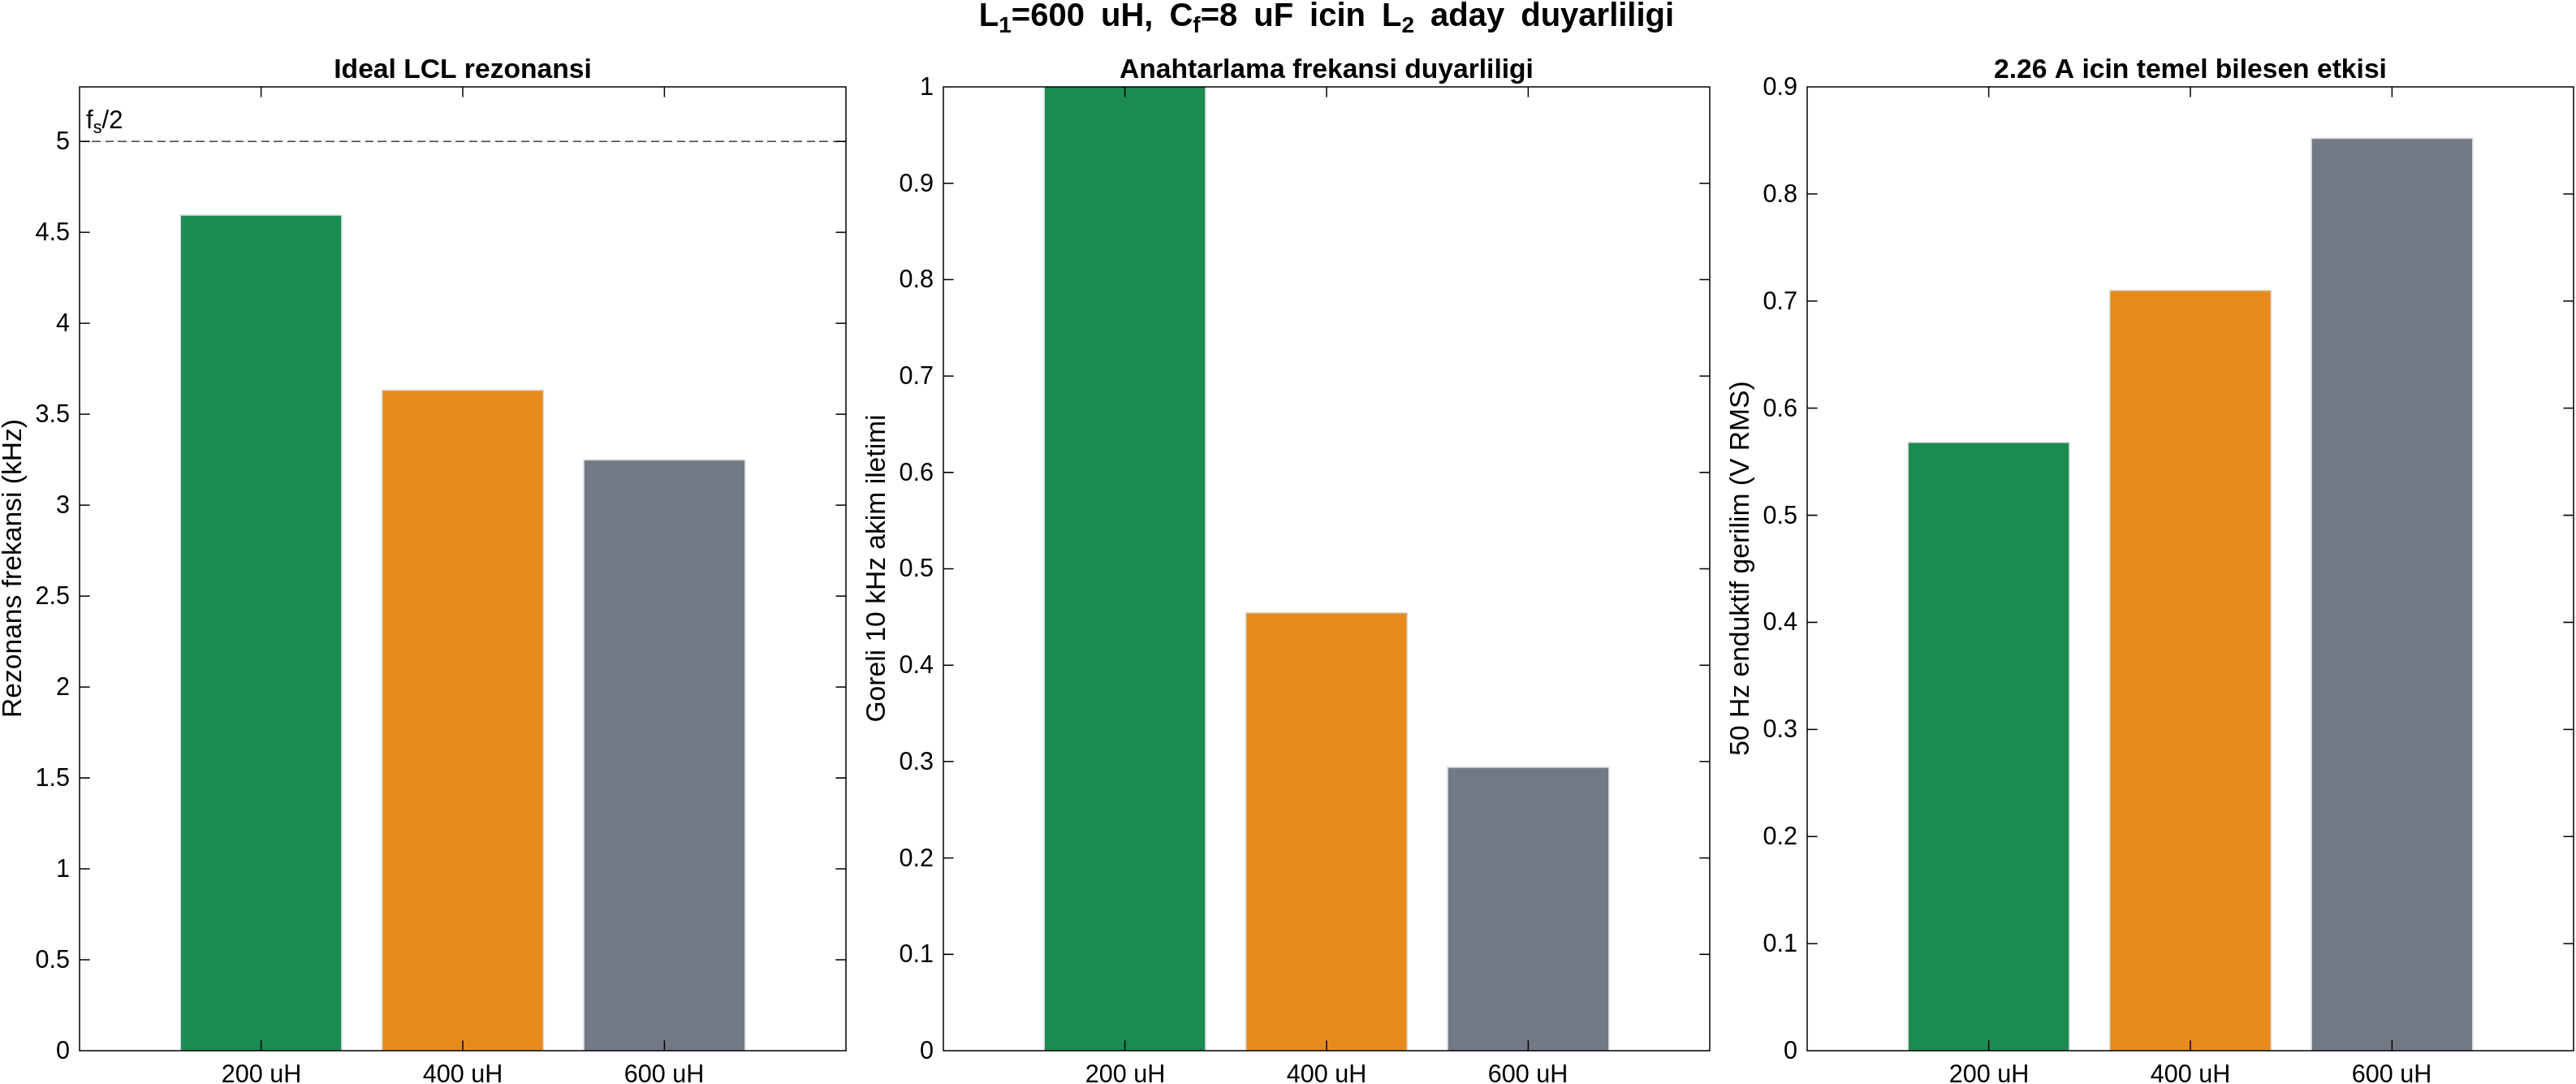
\includegraphics[width=\textwidth]{sonuclar/l2_aday_degerlendirme_20260826.png}
  \caption{$L_1=\SI{600}{\micro\henry}$ ve $C_f=\SI{8}{\micro\farad}$ için $L_2$ aday duyarlılığı: ideal rezonans frekansı, \SI{10}{\kilo\hertz} şebeke akımı iletimi ve \SI{2.26}{\ampere} RMS akımda \SI{50}{\hertz} toplam endüktif gerilim etkisi. Yeşil sütun nihai kaynak seçimini, turuncu eski model ayarını, gri ise faz etiketi olarak ayrıştırılan değeri göstermektedir.}
  \label{fig:l2-aday-degerlendirme}
\end{figure}

\subsection{Yarıiletken Eşlemesi ve Model Katmanları}

Veri sayfaları, blok ekranları ve Senaryo~1 modelinin bağlı elemanları birlikte incelendiğinde, dört IGBT ile harici diyotların aynı ortak parametre kümesiyle temsil edilemeyeceği belirlenmiştir. Faz kolunun dış anahtarları $S_1$--$S_2$ SKM100GB12T4, iç/nötr anahtarları $S_3$--$S_4$ IXYN100N65C3H1, harici $D_1$--$D_2$ diyotları ise DSEI2x61-12B olarak eşlenmiştir. DSEI parametrelerinin IGBT'lerin iç veya ters paralel diyotlarına yayılması fiziksel olarak doğru değildir. Tablo~\ref{tab:yariiletken-esleme}, R2025b çalışma kopyasında kullanılan izlenebilir eşlemeyi vermektedir.

\begin{table}[htbp]
  \centering
  \caption{Senaryo~1 yarıiletkenlerinin parça kodu, model rolü ve R2025b çalışma kopyasındaki eşlemesi.}
  \label{tab:yariiletken-esleme}
  \footnotesize
  \begin{tabularx}{\textwidth}{>{\raggedright\arraybackslash}p{0.13\textwidth} >{\raggedright\arraybackslash}p{0.23\textwidth} >{\raggedright\arraybackslash}p{0.27\textwidth} >{\raggedright\arraybackslash}X}
    \toprule
    Devre rolü & Parça kodu & Bağlı model blokları & Uygulanan kanıt / sınır \\
    \midrule
    $S_1$--$S_2$ dış IGBT & SKM100GB12T4 & \texttt{N-Channel IGBT}, \texttt{N-Channel IGBT4} & Veri sayfasına dayalı doğrulanmış şablondan aktarıldı. \\
    $S_3$--$S_4$ iç IGBT & IXYN100N65C3H1 & \texttt{N-Channel IGBT2}, \texttt{N-Channel IGBT3} & Veri sayfasına dayalı doğrulanmış şablondan aktarıldı. \\
    $D_1$--$D_2$ harici diyot & DSEI2x61-12B & \texttt{Diode6}, \texttt{Diode7} & $V_f=\SI{1.35}{\volt}$, $R_{\mathrm{on}}=\SI{8.5}{\milli\ohm}$ ve verilen ters toparlanma kümesi yalnız bu iki bloğa uygulandı. \\
    IGBT iç/ters paralel diyotları & Aygıta özgü & Diğer bağlı diyot blokları & DSEI ile değiştirilmedi; aygıta özgü davranış korunmalıdır. \\
    \bottomrule
  \end{tabularx}
\end{table}

Tam veri sayfası akım--gerilim ve anahtarlama kaybı tabloları, kısa süreli cihaz stresi ve kayıp teyidi için ayrıntılı model katmanını oluşturur. Kararlı hâl THD ve senaryo taraması ise aynı topoloji ve filtreyi kullanan, fakat cihaz dinamikleri sadeleştirilmiş sistem katmanında yürütülmelidir. İki katmanın sonuçları aynı kanıt olarak birleştirilmeyecek; sistem katmanındaki verim, ayrıntılı cihaz kayıplarıyla çapraz denetlenmeden nihai kabul edilmeyecektir.

\section{Benzetim ve Deneysel Doğrulama Metodolojisi}

Önerilen anahtarlama ve kompanzasyon yöntemleri aynı model, çalışma noktası ve ölçüm tanımları altında karşılaştırılacaktır. Temel karşılaştırma kolları klasik tamamlayıcı anahtarlama, nötr anahtar susturma yöntemi ve Sin\textsuperscript{3} kompanzasyonlu nötr anahtar susturma yöntemi olarak belirlenmiştir. Her kol için aynı DA bara gerilimi, şebeke gerilimi, filtre, anahtarlama frekansı, örnekleme frekansı, denetleyici katsayıları ve veri işleme penceresi kullanılacaktır.

Doğrulama yalnızca düşük güç noktasıyla sınırlandırılmayacaktır. Tablo~\ref{tab:dogrulama-matrisi}; düşük, orta ve anma gücü bölgelerinde karşılaştırılacak yöntemleri, kaydedilecek büyüklükleri ve raporlanacak ölçütleri aynı deney planında birleştirmektedir. Kararlı durum ölçümlerine ek olarak referans basamağı ve şebeke gerilimi değişimi gibi geçici durumların eklenmesi, verim ve THD iyileşmesinin kararlılık veya doyum pahasına elde edilip edilmediğini sınamak için gereklidir. Güvenlik veya donanım sınırları anma gücü deneyini engellerse, erişilebilen en yüksek deney noktası açıkça yazılacak ve kalan bölge doğrulanmış yüksek doğruluklu benzetim ile ayrıştırılacaktır.

\begin{table}[htbp]
  \centering
  \caption{Önerilen karşılaştırmalı doğrulama matrisi.}
  \label{tab:dogrulama-matrisi}
  \small
  \begin{tabularx}{\textwidth}{p{0.19\textwidth} p{0.19\textwidth} X X}
    \toprule
    Çalışma bölgesi & Yöntemler & Kaydedilecek büyüklükler & Raporlanacak ölçütler \\
    \midrule
    Düşük güç & Klasik; susturma; susturma + Sin\textsuperscript{3} & $v_{dc}$, $v_g$, $i_1$, $i_2$, kapı işaretleri, denetleyici çıkışı & Verim, faz ve $L_1$ THD, üçüncü harmonik, ters akım alanı, RMS akım \\
    Orta güç & Aynı üç yöntem & Aynı ölçüm kanalları ve aynı işleme penceresi & Verim, THD, güç faktörü, kontrol eforu, doyum \\
    Anma gücü & En az klasik ve nihai öneri & Akım izleme, sıcaklık, DA bara dengesi, koruma ve geçici rejim & Kapalı çevrim kararlılığı, THD, verim, doyum ve güvenli çalışma \\
    Geçici rejim & Referans/güç basamağı ve gerilim değişimi & Referans, ölçülen akım, modülasyon komutu, hata/koruma işaretleri & Yerleşme süresi, aşım, akım sınırı ve yeniden toparlanma \\
    \bottomrule
  \end{tabularx}
\end{table}

Karşılaştırmaların aynı tanımlarla tekrarlanabilmesi için pencere başlangıcı $t_0$ ve kararlı durum analiz süresi $T_w$ olarak tanımlansın. DA bara gerilimi ile akımı $v_{\mathrm{dc}}$ ve $i_{\mathrm{dc}}$; şebeke tarafı faz gerilimleri ile akımları $v_{g,a},v_{g,b},v_{g,c}$ ve $i_{g,a},i_{g,b},i_{g,c}$ ile gösterildiğinde ortalama DA ve üç faz AA güçleri
\begin{equation}
  \begin{aligned}
    P_{\mathrm{dc}} &= \frac{1}{T_w}\int_{t_0}^{t_0+T_w}v_{\mathrm{dc}}(t)i_{\mathrm{dc}}(t)\,\mathrm{d}t, \\
    P_{\mathrm{ac}} &= \frac{1}{T_w}\int_{t_0}^{t_0+T_w}\left[v_{g,a}(t)i_{g,a}(t)+v_{g,b}(t)i_{g,b}(t)+v_{g,c}(t)i_{g,c}(t)\right]\,\mathrm{d}t
  \end{aligned}
  \label{eq:guc-ortalama-tanimlari}
\end{equation}
olarak hesaplanacaktır. Eşitlik~\eqref{eq:guc-ortalama-tanimlari} için akım yönleri, deşarj sırasında $P_{\mathrm{dc}}>0$ ve şebekeye aktarılan güç için $P_{\mathrm{ac}}>0$ olacak biçimde seçilecektir. Deşarj yönündeki yüzde verim
\begin{equation}
  \eta=100\frac{P_{\mathrm{ac}}}{P_{\mathrm{dc}}}
  \label{eq:verim-tanimi}
\end{equation}
biçiminde raporlanacaktır. Eşitlik~\eqref{eq:verim-tanimi}, yalnızca aynı zaman penceresinden elde edilen giriş ve çıkış güçlerine uygulanacaktır. Akımın $h$'inci harmonik RMS bileşeni $I_h$, temel bileşen RMS değeri $I_1$, hesaba katılan en büyük harmonik mertebesi $H$, örnek sayısı $N_s$ ve örnek indisi $k$ ile gösterilsin. Ayrık referans ve ölçülen akım örnekleri $i^{\ast}[k]$ ile $i[k]$ olduğunda akım toplam harmonik bozunumu ve akım izleme hatası
\begin{equation}
  \begin{aligned}
    \mathrm{THD}_i &=100\frac{\sqrt{\sum_{h=2}^{H}I_h^2}}{I_1}, \\
    \mathrm{RMSE}_i&=\sqrt{\frac{1}{N_s}\sum_{k=1}^{N_s}\left(i^{\ast}[k]-i[k]\right)^2}
  \end{aligned}
  \label{eq:thd-rmse-tanimlari}
\end{equation}
ile belirlenecektir \citep{Teodorescu2011,IEC61000}. Eşitlik~\eqref{eq:thd-rmse-tanimlari} kullanılırken pencere uzunluğu, pencereleme fonksiyonu ve örnekleme frekansı her sonuçla birlikte kaydedilecektir.

Önerilen yöntemin fiziksel hedefini yalnızca THD üzerinden değerlendirmemek için referans akıma ters endüktör akımının büyüklük--zaman etkisini veren ters akım alanı $A_{\mathrm{rev}}$ ve $j$ numaralı anahtarın ikili kapı durumu $q_j[k]\in\{0,1\}$ üzerinden geçiş sayısı $N_{\mathrm{sw},j}$ tanımlansın. İşaret fonksiyonu $\operatorname{sgn}(\cdot)$ kullanılarak
\begin{equation}
  \begin{aligned}
    A_{\mathrm{rev}} &= \int_{t_0}^{t_0+T_w}\max\!\left[-i_L(t)\operatorname{sgn}\!\left(i^{\ast}(t)\right),0\right]\,\mathrm{d}t, \\
    N_{\mathrm{sw},j} &= \sum_{k=2}^{N_s}\left|q_j[k]-q_j[k-1]\right|,
    \qquad q_j[k]\in\{0,1\}
  \end{aligned}
  \label{eq:ters-akim-anahtarlama-olcutleri}
\end{equation}
tanımları kullanılacaktır. Eşitlik~\eqref{eq:ters-akim-anahtarlama-olcutleri} içindeki $N_{\mathrm{sw},j}$ açma ve kapama kenarlarını ayrı geçişler olarak sayar; anahtarlama çevrimi istenirse değer uygun kenar eşleştirmesiyle ayrıca hesaplanmalıdır. Söz konusu ölçütler, verim değişiminin gerçekten ters enerji dolaşımı ve azalan anahtarlama etkinliğiyle ilişkili olup olmadığını sınamak için kullanılacaktır.

Verim hesabında DA giriş gücü ile AA çıkış gücü eşzamanlı veya zaman farkı açıkça sınırlandırılmış kayıtlar üzerinden karşılaştırılmalıdır. Mevcut deney altyapısında DA ve AA analizörleri arasındaki en yüksek kayıt gecikmesi yaklaşık \SI{50}{\milli\second}, haberleşme çevrimi ise \SI{1}{\second} düzeyindedir. Geçici rejim değerlendirmesi için söz konusu haberleşme kayıtları yeterli değildir; osiloskop veya eşzamanlı veri toplama kaydı kullanılmalıdır. THD hesabında pencere uzunluğu, temel frekans, örnekleme frekansı, harmonik üst sınırı ve analiz edilen kanal açıkça yazılacaktır.

Deneysel kanıt zinciri ham kayıt, işleme betiği veya hesap yöntemi, üretilen tablo/şekil ve tezdeki iddia arasında izlenebilir bağlantı kurmalıdır. Her sonuç şeklinin dosya adı, çalışma noktası, kullanılan yöntem, ölçüm cihazı ve tarih bilgisi bir deney kayıt tablosunda tutulacaktır.

\section{Bölüm Sonucu}

Sistem mimarisi güç, ölçüm ve denetim yollarını ayıracak biçimde tanımlanmış; T-tipi faz kolunun üç gerilim seviyesi ve dört temel akım yolu ortak gösterim altında toplanmıştır. Düşük modülasyon bölgesinde senkron-buck eşdeğeri üzerinden ters akım eşiği açıklanmış, LCL filtre için durum denklemleri ve ideal aktarım fonksiyonu kurulmuştur. Sin\textsuperscript{3} terimi ana katkıyı gölgeleyen bağımsız bir kontrol stratejisi olarak değil, nötr anahtar susturma yöntemini tamamlayan ikincil kompanzasyon yolu olarak konumlandırılmıştır.

Genel blok diyagram, model katmanları tablosu, ortak tabanlı vektör çalışma modları, faz başına LCL ölçüm şeması, işlevsel denetim blok diyagramı, birleşik parametre tablosu ve düşük--orta--anma gücü doğrulama matrisi bölümde tek referans noktası olarak toplanmıştır. Verim, THD, izleme hatası, ters akım alanı ve anahtarlama geçiş sayısı aynı yöntem altında matematiksel olarak tanımlanmıştır. Eksik elektriksel ve denetim değerleri açıkça işaretlenmiş; sonraki adımda kaynak kod, benzetim dosyası, devre şeması ve ham deney kayıtları üzerinden doldurulacak alanlar ayrıştırılmıştır. Kurulan model, sonraki bölümlerde önerilen anahtarlama yönteminin analizi ile Sin\textsuperscript{3} kapalı çevrim/Bode incelemesine temel oluşturmaktadır.

\chapter{DÜŞÜK GÜÇ ANALİZİ VE YENİ ANAHTARLAMA YÖNTEMİ}
\label{chap:anahtarlama}

T-tipi dönüştürücünün düşük güç bölgesindeki davranışı, yalnızca aktarılan aktif gücün azalmasıyla açıklanamaz. Modülasyon indeksinin küçülmesi aktif gerilim durumlarının süresini azaltırken sıfır durumunun ve nötr kol üzerinden gerçekleşen serbest dolaşımın payını artırır. Endüktör akımı bir anahtarlama periyodu içinde sıfıra ulaştığında klasik senkron anahtarlama ters yönde akıma izin verebilir. Yararlı çıkış gücüne katkı sağlamayan ters akım, yarı iletkenlerin ve filtre elemanlarının RMS akımını artırarak hafif yük verimini düşürür. Ters akım yolunun kesilmesi ise süreksiz iletime ve akım dalga biçiminde özellikle üçüncü harmonik bileşenin büyümesine neden olabilir. Düşük güçteki temel tasarım problemi bu iki etki arasındaki ödünleşimin yönetilmesidir.

Bölüm~\ref{chap:sistem} altında T-tipi faz kolunun gerilim durumları, akım yolları ve LCL filtre modeli tanımlanmıştır. Mevcut bölümde aynı fiziksel model kullanılarak ters akımın oluşumu incelenmekte, klasik anahtarlama ile önerilen nötr anahtar susturma yöntemi karşılaştırılmakta ve eldeki üç benzetim senaryosu kanıt düzeyleri açıkça belirtilerek değerlendirilmektedir.

Düşük güç bölgesi yalnız laboratuvar için seçilmiş bir test noktası değildir: fotovoltaik eviricilerde gün doğumu ve gün batımı çevresinde, enerji depolama sistemlerinde ise düşük akımlı şarj veya deşarj komutlarında ortaya çıkan gerçek bir işletme koşuludur. Fotovoltaik üretim profilleri ile saha ölçümlerinde kısmi yük süresinin ve düşük akımdaki THD artışının gösterilmesi bu işletme gerekçesini desteklemektedir \citep{Mondol2007,AbRahman2020,Chicco2009}. Enerji depolama uygulamalarında çift yönlü güç komutunun geniş bir aralıkta değişebilmesi de dönüştürücünün yalnız anma noktasında değerlendirilmemesini gerektirir \citep{Aneke2016}.

\section{Ters Akım Dolaşım Mekanizması}

Şebekeye verilen faz akımının temel bileşeni $i_g(t)=\hat I_g\sin(\omega_0t)$ olarak ele alınsın. Düşük güçte $\hat I_g$ küçülürken anahtarlama dalgalanmasının genliği aynı oranda küçülmeyebilir. Bölüm~\ref{chap:sistem} içinde verilen Eşitlik~\eqref{eq:ters-akim-esigi} koşuluna göre ortalama endüktör akımının dalgalanmanın yarısından küçük olması, akımın anahtarlama periyodu içerisinde sıfırı geçebilmesine yol açar. Klasik diyotlu alçaltıcı dönüştürücüde akım sıfıra ulaştığında serbest dolaşım diyodu doğal olarak kesime gider. Senkron yapıda diyoda paralel anahtar iletimde tutulduğu için aynı doğal kesim gerçekleşmez \citep{Erickson2001,Chen2010}.

T-tipi faz kolunun nötr durumu, pozitif ve negatif yarım periyotlarda senkron alçaltıcı dönüştürücünün serbest dolaşım durumuna benzer bir görev üstlenir. Faz akımı referans yönünde azalarak sıfıra ulaştığında nötr kol iletimde kalırsa LCL filtre kapasitöründe ve şebeke eşdeğerinde bulunan enerji ters yönde akım oluşturabilir. Akımın işaret değiştirdiği söz konusu aralıkta enerji şebekeden veya filtre kapasitöründen nötr noktaya doğru taşınır. Aktarılan ortalama aktif gücü artırmayan dolaşım akımı, iletim ve bakır kayıpları açısından ek yük oluşturur. Genel senkron-buck dönüştürücüde diyot benzetimi ile zorlanmış sürekli iletimin farkı Şekil~\ref{fig:de-ccm-akim} üzerinde birincil kaynakla gösterilmişti; mevcut bölüm aynı hafif-yük davranışını T-tipi faz kolunun nötr durumuna ve ölçülebilir ters akım yüküne uyarlamaktadır \citep{Erickson2001,Mohan2003,Chen2010}.

Klasik senkron buck dönüştürücülerde tamamlayıcı sürme, MOSFET kanalı üzerinden diyot kaybını azaltabilir; incelenen T-tipi yapının nötr kolunda IGBT kullanılması nedeniyle aynı kazanç daha sınırlı kalabilir. Nötr IGBT'lerin iki yönlü akımı sürdürmesiyle oluşan ters dolaşım, düşük güçte tamamlayıcı sürmenin olası iletim avantajını aşan bir kayıp mekanizmasına dönüşebilir. Kesin kayıp karşılaştırması için IGBT ve diyot iletim karakteristikleriyle anahtarlama kayıplarının gerçek parça kodları üzerinden hesaplanması gerekmektedir.

Bir temel periyot $T_0$, faz kolu endüktör akımı $i_L(t)$, istenen enerji aktarım yönünü veren akım referansı $i^{\ast}(t)$ ve işaret fonksiyonu $\operatorname{sgn}(\cdot)$ ile gösterilsin. Referans yönüne ters akımın akım--zaman büyüklüğünü veren ters akım yükü $Q_{\mathrm{rev}}$
\begin{equation}
  Q_{\mathrm{rev}}=\int_0^{T_0}\max\!\left[-i_L(t)\,\operatorname{sgn}\!\left(i^{\ast}(t)\right),0\right]\,\mathrm{d}t
  \label{eq:ters-akim-yuku}
\end{equation}
ile tanımlanabilir. Eşitlik~\eqref{eq:ters-akim-yuku} akımın mutlak yönü yerine referansa göre ters bileşeni seçer ve amper--saniye birimindedir; tek başına kayıp enerjisi veya gücü vermez, farklı anahtarlama yöntemlerindeki dolaşımı karşılaştırmak için kullanılır. Parçalı doğrusal yarı iletken modelinde sabit iletim gerilimi $V_{\mathrm{on}}$, eğim direnci $R_{\mathrm{on}}$, iletimdeki mutlak akım ortalaması $I_{\mathrm{avg,abs}}$ ve RMS akım $I_{\mathrm{rms}}$ ile basitleştirilmiş iletim kaybı
\begin{equation}
  P_{\mathrm{cond}}\simeq V_{\mathrm{on}} I_{\mathrm{avg,abs}}+R_{\mathrm{on}}I_{\mathrm{rms}}^2
  \label{eq:iletim-kaybi-yaklasik}
\end{equation}
ile yaklaştırılabilir \citep{Chen2010,Schweizer2013}. Eşitlik~\eqref{eq:iletim-kaybi-yaklasik} anahtarlama enerjisini ve sıcaklık bağımlılığını içermeyen ilk mertebe bir iletim modelidir. Ortalama aktif gücü değiştirmeyen bir ters akım bile $I_{\mathrm{rms}}$ değerini ve kaybı büyütebilir; nötr kol anahtarları, filtre endüktansları ve bağlantı iletkenleri aynı RMS artışından etkilenir.

Kayıp dağılımının düşük güçteki değişimi de Eşitlik~\eqref{eq:iletim-kaybi-yaklasik} üzerinden yorumlanabilir. Düşük akımda $V_{\mathrm{on}}I_{\mathrm{avg,abs}}$ teriminin aktarılan çıkış gücüne oranı büyüdüğünden, yüksek güçte ikincil kalan sabit iletim gerilimi düşümü hafif yük veriminde belirginleşir. Modülasyon indeksi küçüldükçe ana güç anahtarlarının aktif durum payı azalırken nötr durumda geçirilen sürenin artması, toplam kaybın ana anahtarlardan nötr kol elemanlarına ve serbest dolaşım yollarına doğru yeniden dağılmasına yol açar. Sayısal dağılım henüz sonuç olarak verilmemiştir; anahtar başına iletim süresi, RMS akım, gerçek $V_{\mathrm{CE(sat)}}$/diyot karakteristiği ve geçiş enerjileri kesin model veya parça kodları üzerinden hesaplanacaktır \citep{Schweizer2013,Wang2020,Chen2010}.

Ters akımın yalnız akım işaretine bakılarak belirlenmesi yeterli değildir. Ölçüm gürültüsü, akım sensörü ofseti, PWM güncelleme gecikmesi, ölü zaman ve anahtarlama anındaki diyot iletimi sıfır geçiş çevresinde yanlış karar üretebilir. Güvenilir uygulama; akım eşiği, histerezis, minimum bekleme süresi ve güvenli komütasyon koşullarını birlikte kullanmalıdır. Gerçek kapı kodu mevcut olmadığından söz konusu değerler tezde sayısal olarak varsayılmamış, doğrulama gerektiren tasarım değişkenleri olarak bırakılmıştır. Akım denetleyicisinin özellikle sıfır geçiş çevresinde referans--ölçüm farkını azaltmak için oluşturduğu düzeltmeler, ana güç anahtarları ile nötr kol arasındaki geçiş sayısını da artırabilir; yeni doğrulamada kapı başına $N_{\mathrm{sw},j}$ geçiş sayısı, kontrol eforu ve ters akım alanı aynı analiz penceresinde birlikte ölçülecek, verim değişiminin ters dolaşımdan mı, ek anahtarlamadan mı yoksa iki etkiden birlikte mi kaynaklandığı Eşitlik~\eqref{eq:ters-akim-anahtarlama-olcutleri} üzerinden sınanacaktır \citep{Teodorescu2006PR,Zhang2014Deadtime}.

\section{Senkron Buck Eşdeğer Modeli}

Pozitif yarım periyotta faz kolu $P$ ve $O$, negatif yarım periyotta $N$ ve $O$ durumları arasında anahtarlanır. Her yarım periyot kendi işaretine göre ele alındığında yapı iki senkron buck dönüştürücünün simetrik birleşimi olarak yorumlanabilir \citep{Mohan2003,Erickson2001,Holmes2003}. Ortalama akım ile akım dalgalanması arasındaki ilişki üç çalışma bölgesi oluşturur:

\begin{enumerate}
  \item \textbf{Sürekli iletim bölgesi:} $|\bar i_L|>\Delta i_L/2$ koşulunda akım bir anahtarlama periyodu içinde sıfıra ulaşmaz. Senkron nötr anahtarın iletim gerilim düşümünü azaltması verim açısından yararlıdır.
  \item \textbf{Sınır iletim bölgesi:} $|\bar i_L|\simeq\Delta i_L/2$ noktasında akım periyot sonunda sıfıra yaklaşır. Parametre belirsizlikleri ve gecikmeler nedeniyle yöntem geçişi için histerezis gereklidir.
  \item \textbf{Zorlanmış sürekli iletim bölgesi:} $|\bar i_L|<\Delta i_L/2$ olmasına rağmen senkron anahtarlama sürdürülürse akım sıfırın ötesine geçer. Ters akım kaybı belirginleşirken akımın sürekliliği harmonik performansı destekleyebilir.
\end{enumerate}

Sınır akımı yaklaşık olarak
\begin{equation}
  I_{\mathrm{B}}(t)=\frac{\Delta i_L(t)}{2}
  \label{eq:sinir-akimi}
\end{equation}
şeklinde tanımlanabilir. Eşitlik~\eqref{eq:sinir-akimi} içindeki $I_{\mathrm{B}}$; DA bara gerilimi, anlık şebeke gerilimi, görev oranı, anahtarlama frekansı ve eşdeğer endüktansa bağlıdır. Sabit bir yüzde güç eşiği yerine fiziksel değişkenlerden türetilen sınır akımının kullanılması, şebeke gerilimi veya DA bara seviyesi değiştiğinde daha tutarlı bir kip geçişi sağlayabilir. Nihai $I_{\mathrm{B}}$ sayısı, gerçek eşik/histerezis değerleri kodla kilitlendiğinde verilecektir.

Senkron-buck eşdeğerinin sağladığı temel kazanım, üç fazlı sistemdeki düşük güç davranışını faz kolu düzeyinde enerji aktarımı, serbest dolaşım ve akım sürekliliği bakımından ayrıştırabilmesidir. Pozitif yarım periyotta üst ana anahtar ile nötr kolun, negatif yarım periyotta ise alt ana anahtar ile karşı nötr yolun görevleri aynı devre modeli üzerinde izlenebilir. Eşdeğer model böylece modülasyon indeksinin küçülmesiyle nötr durum payının artmasını, endüktör akımının sıfırı geçmesini ve hangi kapı geçişlerinin ek anahtarlama yükü oluşturduğunu ortak bir fiziksel çerçeveye bağlar; sınır akımı, ters akım alanı ve anahtar geçiş sayısı ölçütlerinin kurulmasına da temel oluşturur.

\section{Klasik Anahtarlama Yöntemi}

Klasik üç seviyeli modülasyonda nötr kol, sıfır gerilim durumunu üretmek üzere her iki yarım periyotta etkin kullanılır. Pozitif alternansta aktif enerji aktarımı $P$ durumu, serbest dolaşım $O$ durumu; negatif alternansta aktif enerji aktarımı $N$ durumu, serbest dolaşım yine $O$ durumu üzerinden gerçekleşir. Akım referansı küçüldüğünde aktif durumun görev oranı azalır ve nötr durumda geçirilen süre uzar.

İncelenen benzetim kurgusunda üç fazlı, dört telli yapının her fazı bağımsız bir tek fazlı T-tipi kol olarak ele alınmış ve kapı işaretleri sinüzoidal PWM (SPWM) ile üretilmiştir. Faz başına inceleme, nötr anahtar müdahalesinin hangi yarım periyotta ve hangi kol üzerinde yapıldığını açıkça göstermektedir. Yöntemin uzay vektör PWM veya başka modülasyon tekniklerine genellenmesi, mevcut kanıtın dışında kalan ayrı bir doğrulama konusudur.

Senkron anahtarlamanın temel üstünlüğü, normal ve yüksek akım bölgesinde diyot iletimini düşük gerilim düşümlü anahtar kanalıyla değiştirebilmesidir. Aynı davranış düşük güçte nötr kolun akımı iki yönde de iletebilmesi nedeniyle dezavantaja dönüşür. Akım sıfıra ulaştıktan sonra kapı komutunun korunması, akım yönünü sınırlayan doğal bir diyot kesimi bırakmaz. Klasik yöntem bu yüzden düşük THD sağlayabilmesine karşın hafif yükte ters akım alanı ve RMS akım bakımından elverişsizdir. İki yöntemin işlevsel farkı Tablo~\ref{tab:klasik-onerilen-islevsel} üzerinde özetlenmiştir.

\begin{table}[htbp]
  \centering
  \caption{Klasik ve önerilen anahtarlamanın düşük güçte işlevsel karşılaştırması.}
  \label{tab:klasik-onerilen-islevsel}
  \small
  \begin{tabularx}{\textwidth}{p{0.22\textwidth} X X}
    \toprule
    Özellik & Klasik senkron anahtarlama & Önerilen nötr anahtar susturma \\
    \midrule
    Sıfır durumu & Nötr kol iki yönlü akıma izin verir. & Ters dolaşıma yol açan nötr komutu düşük güç bölgesinde engellenir. \\
    Akım sürekliliği & Sıfır geçişten sonra ters yönde sürdürülebilir. & Akım sıfırda doğal olarak kesilebilir; süreksiz iletim oluşabilir. \\
    Beklenen kayıp etkisi & Ters akım nedeniyle RMS ve iletim kaybı artabilir. & Ters akım yolu azaltıldığı için iletim kaybı düşebilir. \\
    Beklenen harmonik etkisi & Akım sürekliliği THD açısından avantaj sağlayabilir. & Üçüncü harmonik ve THD belirgin biçimde artabilir. \\
    Gerekli tamamlayıcı önlem & Özel düşük güç müdahalesi yoktur. & Sin\textsuperscript{3} kompanzasyonu ve güvenli kip geçişi gerekir. \\
    \bottomrule
  \end{tabularx}
\end{table}

\section{Önerilen Anahtarlama Yöntemi}

Önerilen yöntemin amacı, düşük güçte referans enerji yönüne ters akımı sürdüren nötr anahtar komutunu bastırmaktır. Yöntem klasik PWM yapısını tüm çalışma aralığında değiştirmemekte, yalnız akımın sınır iletim bölgesine yaklaştığı koşullarda devreye girmektedir. Yarım periyot işareti, akım referansı ve ölçülen akım birlikte değerlendirilerek yararlı akım yönünün tersine iletime yol açan nötr komut belirlenir.

İkili etkinleştirme değişkeni $\sigma(t)\in\{0,1\}$, düşük güç geçiş eşiği $I_{\mathrm{th}}$, pozitif histerezis genişliği $H$ ve ters iletim koşulunu gösteren ikili gösterge $\chi_{\mathrm{rev}}(t)\in\{0,1\}$ ile tanımlansın. Histerezis bandında önceki durumun korunmasını da içeren işlevsel kural
\begin{equation}
  \sigma(t)=
  \begin{cases}
    1, & |i^{\ast}(t)|\leq I_{\mathrm{th}}\ \text{ve }\chi_{\mathrm{rev}}(t)=1,\\
    0, & |i^{\ast}(t)|\geq I_{\mathrm{th}}+H\ \text{veya }\chi_{\mathrm{rev}}(t)=0,\\
    \sigma(t^-), & I_{\mathrm{th}}<|i^{\ast}(t)|<I_{\mathrm{th}}+H\ \text{ve }\chi_{\mathrm{rev}}(t)=1
  \end{cases}
  \label{eq:susturma-etkinlestirme}
\end{equation}
ile gösterilebilir. Eşitlik~\eqref{eq:susturma-etkinlestirme} içindeki $t^-$ karar anından hemen önceki durumu gösterir; histerezis aralığında durum korunarak sürekli kip değiştirme önlenir. Klasik ve yeni nötr kapı komutları $g_{n,\mathrm{kl}}(t)$ ile $g_{n,\mathrm{yeni}}(t)$ olarak tanımlandığında
\begin{equation}
  g_{n,\mathrm{yeni}}(t)=g_{n,\mathrm{kl}}(t)\left[1-\sigma(t)\chi_{\mathrm{rev}}(t)\right]
  \label{eq:notr-susturma-kurali}
\end{equation}
biçiminde özetlenebilir. Eşitlik~\eqref{eq:notr-susturma-kurali} gerçek sürücüye doğrudan aktarılacak kesin bir kapı tablosu değil, yöntemin hangi komutu hangi amaçla değiştirdiğini belirleyen işlevsel tanımdır. Anahtarların gerçek adları, polariteleri ve güvenli komütasyon sırası kaynak kod veya sürücü kaydı bulunmadan kesinleştirilemez.

Klasik ve nötr anahtar susturmalı yöntemlerin kapı komutları, benzetim kayıtlarında hem tam temel periyot hem de seçilmiş anahtarlama penceresinin yakın görünümüyle belgelenmiştir. Klasik yöntem Şekil~\ref{fig:klasik-kapi-darbeleri-tam} ve Şekil~\ref{fig:klasik-kapi-darbeleri-yakin}, önerilen yöntem Şekil~\ref{fig:susturma-kapi-darbeleri-tam} ve Şekil~\ref{fig:susturma-kapi-darbeleri-yakin} altında verilmektedir; dört kayıt aynı içeriğin tekrarı olmadığından birleştirilmemiştir.

\begin{figure}[htbp]
  \centering
  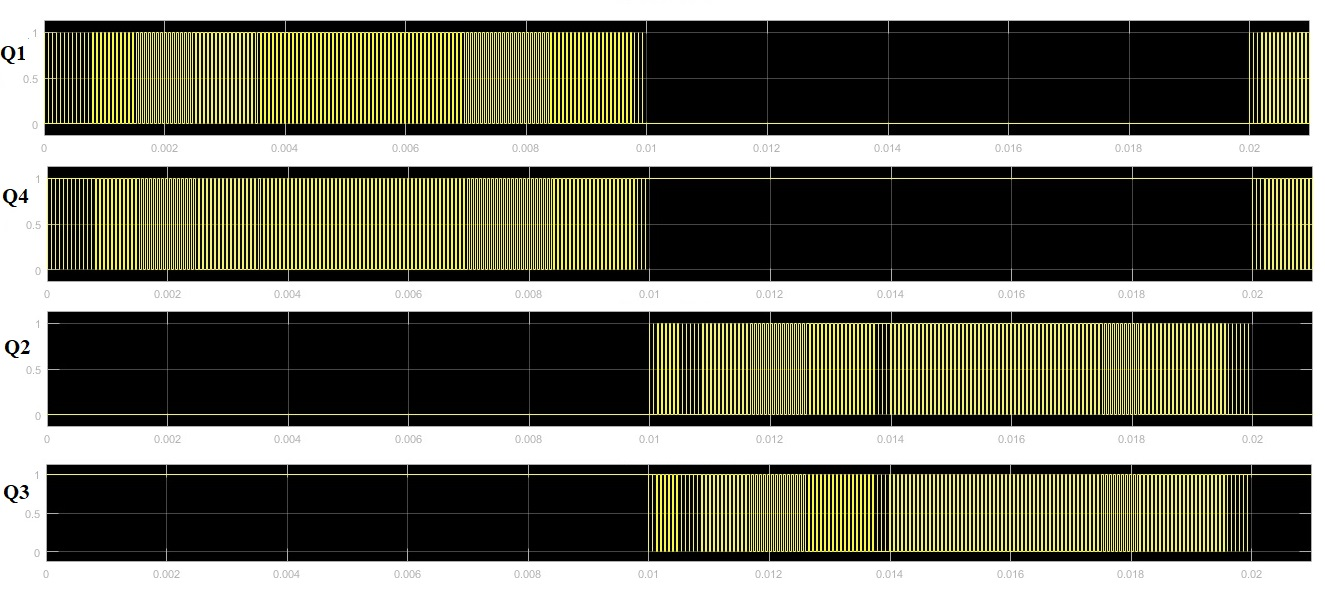
\includegraphics[width=0.98\textwidth]{sistem/onceki_tez_klasik_kapi_darbeleri.jpg}
  \caption{Klasik tamamlayıcı anahtarlamada $Q_1$--$Q_4$ kapı darbelerinin bir temel periyot boyunca görünümü (benzetim kaydı).}
  \label{fig:klasik-kapi-darbeleri-tam}
\end{figure}

\begin{figure}[H]
  \centering
  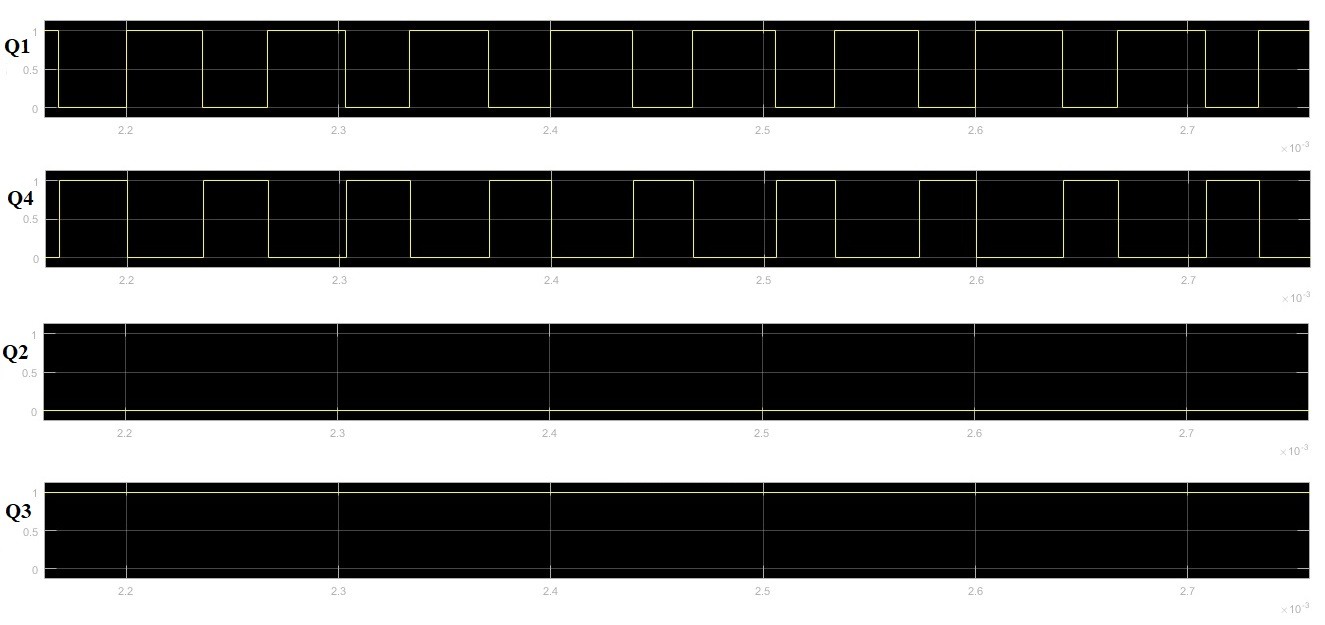
\includegraphics[width=0.98\textwidth]{sistem/onceki_tez_klasik_kapi_darbeleri_yakin.jpg}
  \caption{Klasik tamamlayıcı anahtarlamada seçilmiş anahtarlama penceresinin yakın görünümü (benzetim kaydı).}
  \label{fig:klasik-kapi-darbeleri-yakin}
\end{figure}

Şekil~\ref{fig:klasik-kapi-darbeleri-yakin} altındaki pozitif alternans kesitinde $Q_1$ ile $Q_4$ tamamlayıcı darbelerle anahtarlanırken $Q_2$ kesimde, $Q_3$ iletimde tutulmaktadır. Aynı zaman aralığında önerilen yöntemi gösteren Şekil~\ref{fig:susturma-kapi-darbeleri-yakin} altında $Q_1$ anahtarlamayı sürdürmekte, nötr kola ait $Q_4$ komutu ise sıfırda tutulmaktadır; simetrik olarak negatif alternansta $Q_3$ komutu bastırılmaktadır. Ekran kayıtları ölü zamanı, minimum darbe genişliğini, lojik polariteyi ve sürücü gecikmesini doğrulayamadığından kesin kapı tablosu gerçek PWM koduyla kilitlenecektir.

Benzetim modelinin faz kolu ve tüm sistem ekranı, sonuç dalga biçimlerinden ayrı kanıt türleridir. Şekil~\ref{fig:onceki-faz-modeli}, $Q_1$--$Q_4$, bölünmüş DA bara, $L_1$, $C_1$ ve $L_2$ elemanlarının kullanılan tek fazlı T-tipi kola bağlantısını; Şekil~\ref{fig:onceki-simulasyon-modeli} ise ölçüm, filtre, şebeke eşdeğeri ve güç hesabı bloklarını içeren üst düzey Simulink çalışma alanını göstermektedir. Eldeki Senaryo~1 kaynak dosyası bu genel yapıyla uyumludur; ancak R2025b'de kaldırılan ölçüm blokları ve Senaryo~2--3 model/kodlarının yokluğu nedeniyle ekranlar üç senaryonun yeniden üretilebilir ortak model kanıtı değildir.

\begin{figure}[H]
  \centering
  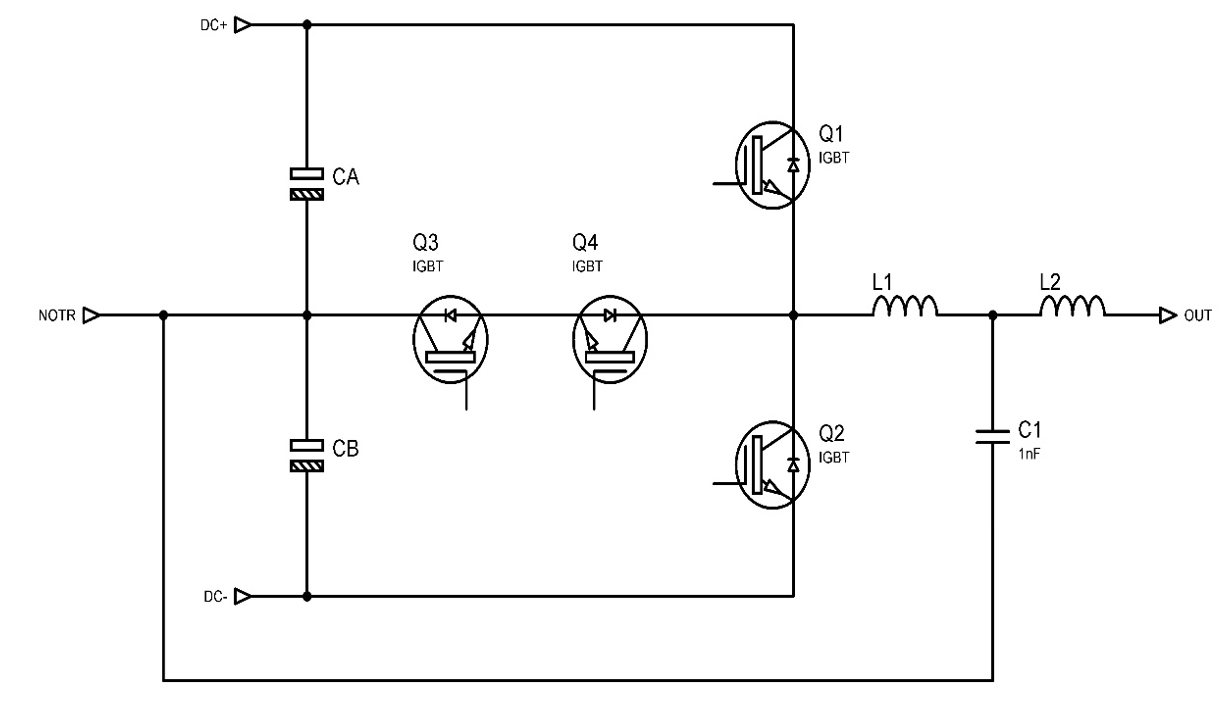
\includegraphics[width=0.90\textwidth]{sonuclar/onceki_tez_t_tipi_faz_modeli.png}
  \caption{Benzetimde kullanılan tek fazlı T-tipi evirici ve LC filtre yapısı.}
  \label{fig:onceki-faz-modeli}
\end{figure}

\begin{figure}[H]
  \centering
  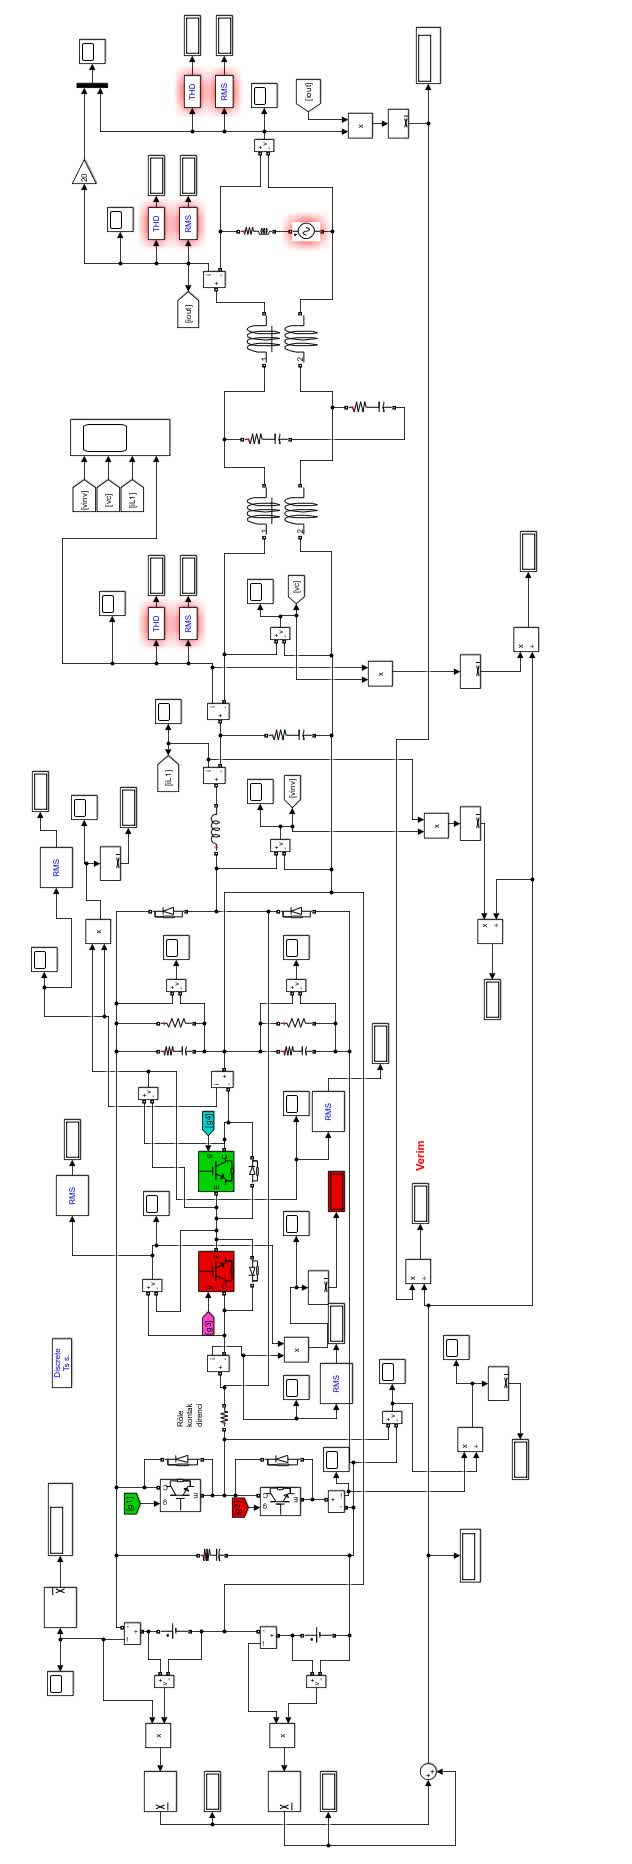
\includegraphics[angle=90,width=0.96\textwidth]{sonuclar/onceki_tez_simulasyon_modeli.jpg}
  \caption{Benzetimde kullanılan Simulink modelinin genel görünümü; Senaryo~1 kaynak modeliyle yapısal olarak uyumludur, üç senaryonun ortak koşulu olarak doğrulanmamıştır.}
  \label{fig:onceki-simulasyon-modeli}
\end{figure}

Güvenli uygulamada dört koşul birlikte sağlanmalıdır. İlk olarak, akım işareti sensör ofsetinden büyük bir güven payıyla belirlenmelidir. İkinci olarak, nötr kolun kesilmesi endüktör akımı için kesintisiz ve aşırı gerilim üretmeyen alternatif bir yol bırakmalıdır. Üçüncü olarak, karşılıklı anahtarların ölü zamanı ve minimum darbe genişliği korunmalıdır. Son olarak, ölçüm geçersizliği veya aşırı akım durumunda denetim önceden tanımlanmış güvenli anahtarlamaya dönmelidir. Eldeki benzetim parametre dosyası ölü zaman içermemektedir; gerçek donanım için ölü zaman ve sürücü gecikmesi ayrıca doğrulanmalıdır \citep{Zhang2014Deadtime}.

Nötr anahtarın bastırılması ters akım yolunu azaltırken endüktör akımını süreksiz iletime zorlar. Akımın sıfır çevresindeki düzleşmesi ve iletim aralıklarının daralması, temel bileşene göre üçüncü harmonik payını büyütür. Süreksiz iletimde akım zarfı, görev oranı ile anahtarlama anındaki endüktör gerilim farkının birlikte değişmesi nedeniyle saf sinüs biçimini koruyamaz: alternans ortasında ($\omega_0t=\pi/2$ ve $3\pi/2$ çevresinde) DA bara ile şebeke gerilimi arasındaki akım yükseltme payının azalması akım zarfında çökme oluşturur; sıfır geçişlerine yakın bölgelerdeki farklı yükselme hızı da üçüncü harmonik bileşeni besler. Önerilen anahtarlama bu yüzden tek başına nihai yöntem değildir; ortaya çıkan harmonik cezanın azaltılması için Bölüm~\ref{chap:sin3} altında incelenen Sin\textsuperscript{3} ileri besleme kompanzasyonu tamamlayıcı katman olarak kullanılmaktadır.

\eksikistek{Kapı mantığı ve senaryo eşlemesinin kodla kesinleştirilmesi}{Senaryo~1 modelinde klasik kapı üretimi görülebilmiştir; ancak R2025b sürüm uyumsuzluğu nedeniyle kaynak koşu tamamlanamamıştır ve Senaryo~2--3 PWM modeli veya kontrol kodu elimizde yoktur. İstiyoruz: (1) Senaryo~2--3 model/kod paketi; (2) dönüştürülmüş ortak modelde $Q_1$--$Q_4$ doğruluk tablosu, tamamlayıcılık, ölü zaman, akım işareti, eşik/histerezis ve kip geçişlerinin yeniden çıkarılması; (3) R2025b diyot yakınsama sorununun giderilip Senaryo~1'in en az iki kararlı \SI{50}{\hertz} periyodu koşturulması.}

\section{Verim ve Harmonik Performans Ödünleşimi}

Eldeki üç senaryo arşivi aynı düşük güç probleminin ardışık karşılaştırma kolları olarak değerlendirilmiştir. Dalga biçimleri ve teknik açıklamalar birlikte incelendiğinde Senaryo~1 klasik senkron anahtarlama, Senaryo~2 nötr anahtar susturma, Senaryo~3 ise susturma ile Sin\textsuperscript{3} kompanzasyonunun birlikte kullanımıyla yüksek ölçüde uyumludur. Yalnız Senaryo~1 için kaynak model mevcuttur; eşleme bu yüzden ``yüksek güvenli'' düzeyde tutulmuş, kesin kod doğrulaması olarak sunulmamıştır.

Benzetim kurgusu; üç fazlı dört telli sistemin faz başına modellenmesini, düşük güç incelemesinin yaklaşık \SI{2.6}{\ampere} RMS faz akımında yapılmasını ve yapısal etkiyi ayırmak için akım denetleyicisinin devre dışı bırakılarak yalnızca ileri besleme katsayısının değiştirilmesini içermektedir. Kontrolörsüz koşullar yöntemin oluşum mekanizmasını ayırmak için yararlıdır; kapalı çevrim performans kanıtı değildir ve Bölüm~\ref{chap:sin3} bu ayrımı ayrıca ele almaktadır.

FFT ekranlarında analiz başlangıcı \SI{0.06}{\second}, pencere uzunluğu iki temel çevrim ve temel frekans \SI{50}{\hertz} olarak verilmiştir. Tablo~\ref{tab:senaryo-thd}, ekranlardan doğrudan okunan değerleri aynı ölçüm tanımı altında toplamaktadır.

\begin{table}[htbp]
  \centering
  \caption{Düşük güç benzetim ekranlarından okunan temel bileşen ve THD değerleri.}
  \label{tab:senaryo-thd}
  \small
  \begin{tabular}{c l S[table-format=1.3] S[table-format=2.2] S[table-format=1.3] S[table-format=2.2]}
    \toprule
    {Senaryo} & {Yöntem eşlemesi} & {$I_{L1,1}$ (A)} & {$\mathrm{THD}_{L1}$ (\%)} & {$I_{\mathrm{out},1}$ (A)} & {$\mathrm{THD}_{\mathrm{out}}$ (\%)} \\
    \midrule
    1 & Klasik anahtarlama & 3.698 & 8.29 & 3.734 & 2.14 \\
    2 & Nötr anahtar susturma & 3.396 & 46.86 & 3.412 & 46.35 \\
    3 & Susturma + Sin\textsuperscript{3} & 3.752 & 9.46 & 3.766 & 7.79 \\
    \bottomrule
  \end{tabular}
\end{table}

Aynı üç yöntem için verim ve THD değerlerini birlikte veren bir benzetim özeti de mevcuttur; Tablo~\ref{tab:onceki-benzetim-ozeti} bu kaydı ayrı kanıt statüsüyle aktarmaktadır. THD değerleri FFT ekranlarıyla yakından uyuşurken verim yüzdeleri, kayıp hesabının yapıldığı ham model mevcut olmadığından yeniden hesaplanamamıştır.

\begin{table}[htbp]
  \centering
  \caption{Raporlanan benzetim verimi ve akım THD değerleri; verim hesabı ham model beklemektedir.}
  \label{tab:onceki-benzetim-ozeti}
  \begin{tabular}{>{\raggedright\arraybackslash}p{0.43\textwidth}ccc}
    \toprule
    \textbf{Yöntem} & \textbf{Verim (\%)} & \textbf{$\mathrm{THD}_{L1}$ (\%)} & \textbf{$\mathrm{THD}_{faz}$ (\%)} \\
    \midrule
    Klasik tamamlayıcı anahtarlama & 90,45 & 8,30 & 2,10 \\
    Nötr anahtar susturma & 93,00 & 46,90 & 46,30 \\
    Susturma + Sin\textsuperscript{3} & 93,70 & 9,50 & 7,80 \\
    \bottomrule
  \end{tabular}
\end{table}

Senaryo~2'de $I_{L1}$ ve $I_{\mathrm{out}}$ THD değerlerinin sırasıyla \%46,86 ve \%46,35'e çıkması, nötr anahtar susturmanın tek başına oluşturduğu harmonik cezayı göstermektedir. Senaryo~3'te aynı değerlerin \%9,46 ve \%7,79'a gerilemesi, Senaryo~2'ye göre yaklaşık \%79,8 ve \%83,2 bağıl azalma anlamına gelir. Kompanzasyon sonrasında temel akım genliklerinin Senaryo~1 ile yakın seviyeye dönmesi, yöntemin düşük güç akımını bütünüyle bastırmadığını da gösterir. Yine de Senaryo~3 çıkış THD değeri Senaryo~1'in \%2,14 seviyesine ulaşmamıştır; kompanzasyonun iyileştirici fakat ideal olmayan sonucu açıkça korunmalıdır.

Senaryo~1'in yüksek çözünürlüklü kayıtları klasik anahtarlamanın referans davranışını belgelemektedir. Şekil~\ref{fig:klasik-l1-tam}, $L_1$ endüktör akımının bir temel periyot içindeki anahtarlama dalgalanmasını göstermektedir; akım zarfının temel bileşen boyunca değişmesi ve yüksek frekanslı üçgensel dalgalanmanın zarf üzerine binmesi, düşük güçte anlık akımın sıfır çevresine yaklaşabildiğini gösterir.

\begin{figure}[H]
  \centering
  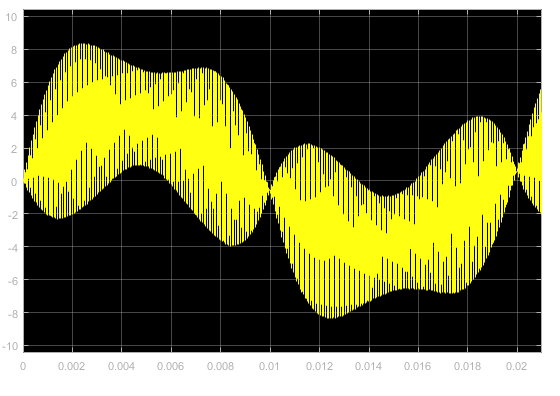
\includegraphics[width=0.82\textwidth]{sonuclar/onceki_tez_l1_tam.png}
  \caption{Klasik anahtarlama benzetiminde $L_1$ endüktör akımının tam-periyot dalga biçimi (Senaryo~1).}
  \label{fig:klasik-l1-tam}
\end{figure}

Şekil~\ref{fig:klasik-l1-yakin}, yaklaşık \SI{0.9}{\milli\second}--\SI{1.8}{\milli\second} aralığını büyüterek akım dalgalanmasının anahtarlama periyodu ölçeğindeki yapısını görünür kılmaktadır. Yaklaşık \SI{10}{\kilo\hertz} anahtarlama frekansıyla uyumlu üçgensel değişim, $L_1$ akımındaki dalgalanmanın yalnız düşük frekanslı zarf üzerinden değerlendirilmemesi gerektiğini gösterir.

\begin{figure}[!htbp]
  \centering
  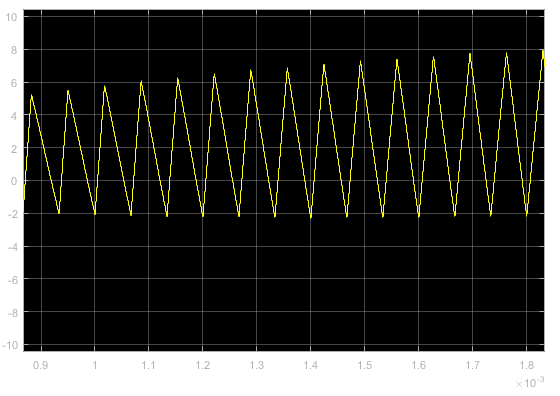
\includegraphics[width=0.82\textwidth]{sonuclar/onceki_tez_l1_yakin_0_9_1_8ms.png}
  \caption{Klasik anahtarlama benzetimindeki $L_1$ endüktör akımından büyütülmüş kesit (Senaryo~1).}
  \label{fig:klasik-l1-yakin}
\end{figure}

Senaryo~1'in dört kanallı kaynak ekranı Şekil~\ref{fig:klasik-dort-kanal} altında verilmiştir. Yukarıdan aşağıya kanallar; anahtarlama devresi çıkışındaki filtre giriş gerilimini, filtrelenmiş gerilimi, $L_1$ endüktör akımını ve LC filtre çıkış akımını göstermektedir. İlk iki kanal anahtarlama geriliminin filtrelenmesini, son iki kanal ise $L_1$ dalgalanmasının çıkış akımında ne ölçüde bastırıldığını aynı zaman ekseninde izlemeyi sağlamaktadır.

\begin{figure}[H]
  \centering
  \includegraphics[width=0.98\textwidth]{../dosyalar/05_sonradan_gelenler/Senaryo_1/dalga_sekli_s1.jpg}
  \caption{Klasik anahtarlamada filtre giriş gerilimi, filtrelenmiş gerilim, $L_1$ endüktör akımı ve LC filtre çıkış akımının birlikte gösterimi (Senaryo~1).}
  \label{fig:klasik-dort-kanal}
\end{figure}

FFT sonuçları, aynı klasik anahtarlama koşulunda filtrenin akım harmonikleri üzerindeki etkisini iki ölçüm noktasında göstermektedir. Şekil~\ref{fig:klasik-l1-fft} altında $L_1$ akımının temel bileşeni \SI{3.698}{\ampere} ve THD değeri \%8,29; Şekil~\ref{fig:klasik-iout-fft} altında çıkış akımının temel bileşeni \SI{3.734}{\ampere} ve THD değeri \%2,14 olarak okunmaktadır. Çıkış akımındaki THD'nin $L_1$ akımına göre yaklaşık \%74,2 azalması, LC filtrenin anahtarlama kaynaklı harmonikleri bastırdığını nicel olarak gösterir.

\begin{figure}[H]
  \centering
  \includegraphics[width=0.98\textwidth]{../dosyalar/05_sonradan_gelenler/Senaryo_1/THD_IL1.jpg}
  \caption{Klasik anahtarlamada $L_1$ endüktör akımının FFT analizi: temel bileşen \SI{3.698}{\ampere}, $\mathrm{THD}_{L1}=\%8{,}29$ (Senaryo~1).}
  \label{fig:klasik-l1-fft}
\end{figure}

\begin{figure}[H]
  \centering
  \includegraphics[width=0.98\textwidth]{../dosyalar/05_sonradan_gelenler/Senaryo_1/THD_Iout.jpg}
  \caption{Klasik anahtarlamada LC filtre çıkış akımının FFT analizi: temel bileşen \SI{3.734}{\ampere}, $\mathrm{THD}_{\mathrm{out}}=\%2{,}14$ (Senaryo~1).}
  \label{fig:klasik-iout-fft}
\end{figure}

Nötr anahtar susturma yöntemine ait kayıtlar yedi ayrı görselden oluşmaktadır: Şekil~\ref{fig:susturma-kapi-darbeleri-tam} ve Şekil~\ref{fig:susturma-kapi-darbeleri-yakin} kapı komutlarını; Şekil~\ref{fig:susturma-l1-tam} ve Şekil~\ref{fig:susturma-l1-yakin} $L_1$ akımını; Şekil~\ref{fig:susturma-dort-kanal} dört ölçüm kanalını; Şekil~\ref{fig:susturma-l1-fft} ile Şekil~\ref{fig:susturma-iout-fft} iki akım ölçüm noktasının FFT sonuçlarını göstermektedir. Görsellerin ayrı tutulması, anahtarlama müdahalesi ile ortaya çıkan akım ve harmonik sonuçları arasındaki neden--sonuç zincirini izlenebilir kılmaktadır.

\begin{figure}[H]
  \centering
  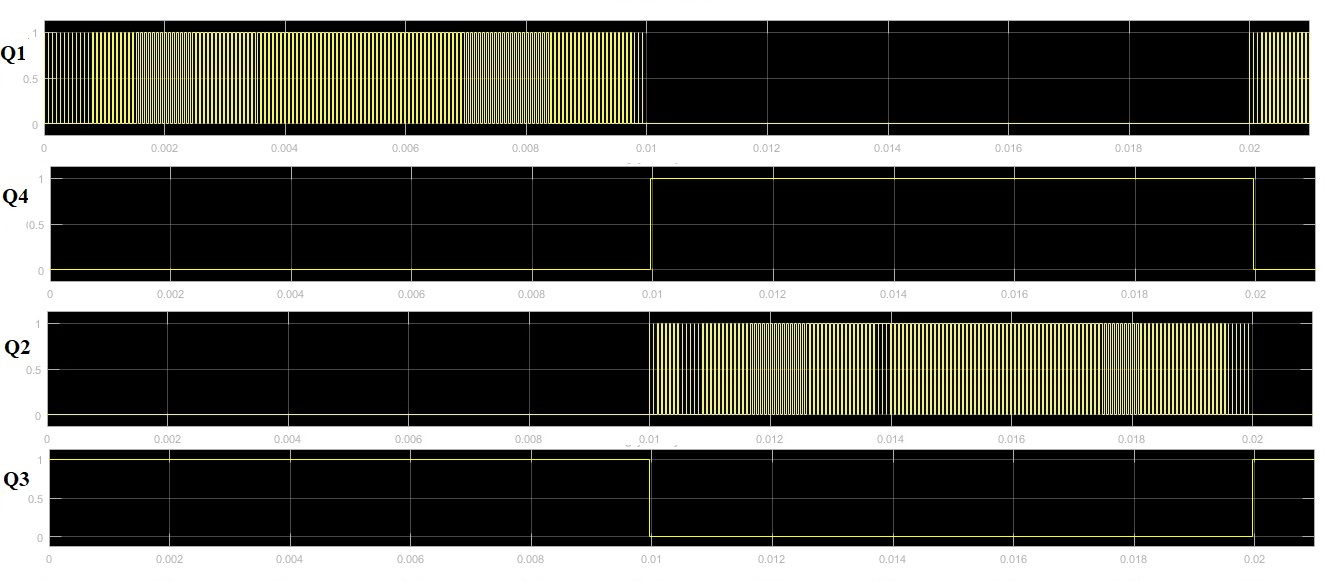
\includegraphics[width=0.98\textwidth]{sistem/onceki_tez_susturma_kapi_darbeleri.jpg}
  \caption{Önerilen nötr anahtar susturma yönteminde $Q_1$--$Q_4$ kapı darbelerinin bir temel periyot boyunca görünümü (Senaryo~2).}
  \label{fig:susturma-kapi-darbeleri-tam}
\end{figure}

Şekil~\ref{fig:susturma-kapi-darbeleri-tam} altında pozitif alternansta $Q_1$ anahtarlamayı sürdürürken $Q_4$ komutunun sıfırda tutulduğu; negatif alternansta simetrik anahtarlama rolünün karşı kola geçtiği görülmektedir. Şekil~\ref{fig:susturma-kapi-darbeleri-yakin}, yaklaşık \SI{2.2}{\milli\second}--\SI{2.7}{\milli\second} aralığında $Q_1$ darbeleri devam ederken $Q_4$ ve $Q_2$ komutlarının sıfırda, $Q_3$ komutunun iletimde kaldığını daha açık göstermektedir.

\begin{figure}[H]
  \centering
  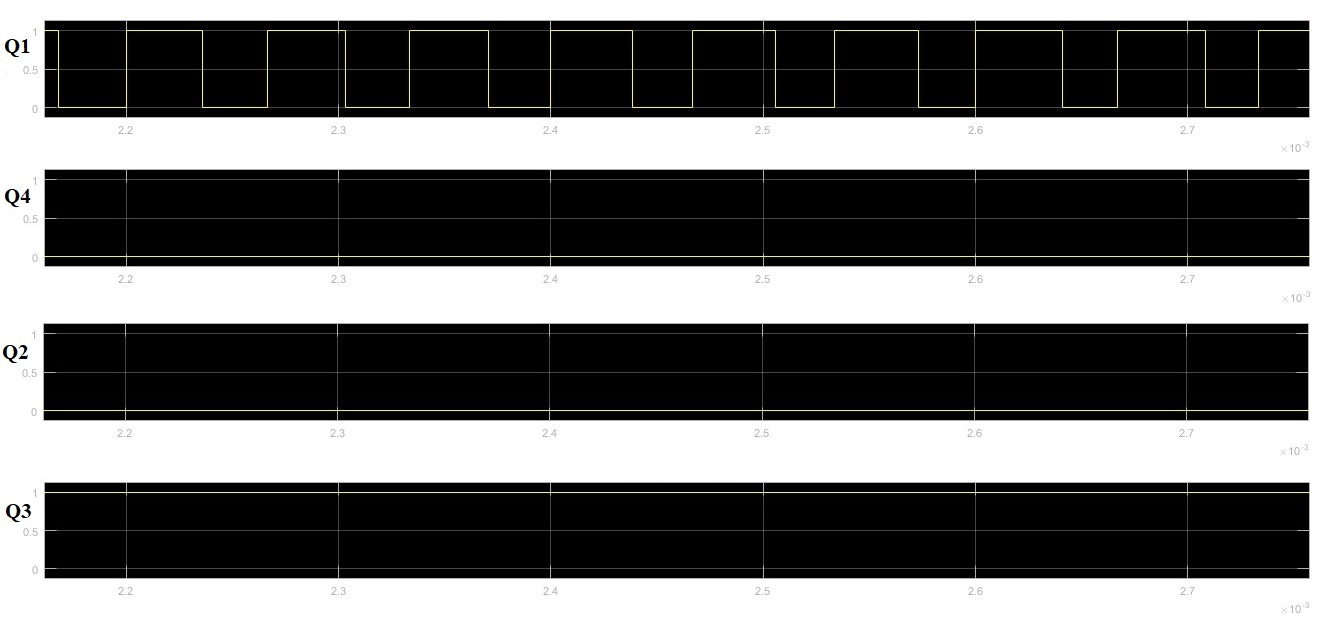
\includegraphics[width=0.98\textwidth]{sistem/onceki_tez_susturma_kapi_darbeleri_yakin.jpg}
  \caption{Önerilen nötr anahtar susturma yönteminde seçilmiş anahtarlama penceresinin yakın görünümü (Senaryo~2).}
  \label{fig:susturma-kapi-darbeleri-yakin}
\end{figure}

Şekil~\ref{fig:susturma-l1-tam}, nötr anahtar susturulduğunda $L_1$ akımının sıfırın ters yönünde sürekli dolaşmak yerine her anahtarlama çevriminde sıfıra oturan aralıklar oluşturduğunu göstermektedir. Klasik yöntemin Şekil~\ref{fig:klasik-l1-tam} altındaki iki yönlü dalgalanmasına karşılık burada görülen sıfır-akım aralıkları süreksiz iletim davranışının doğrudan görsel kanıtıdır.

\begin{figure}[H]
  \centering
  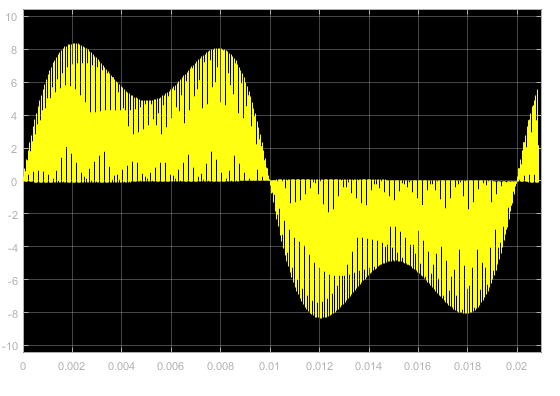
\includegraphics[width=0.82\textwidth]{sonuclar/onceki_tez_susturma_l1_tam.png}
  \caption{Nötr anahtar susturma benzetiminde $L_1$ endüktör akımının tam-periyot dalga biçimi (Senaryo~2).}
  \label{fig:susturma-l1-tam}
\end{figure}

Yakın görünüm Şekil~\ref{fig:susturma-l1-yakin} altında verilmiştir. Akımın pozitif eğimle yükselmesinin ardından sıfıra düşmesi ve bir sonraki çevrime kadar sıfırda kalması, nötr kolun klasik senkron serbest dolaşım yolunu sürdürmediğini göstermektedir. Tepe değerinin temel periyot boyunca değişmesi, süreksiz iletim zarfının saf sinüzoidal biçimde kalmadığını da açıklamaktadır.

\begin{figure}[H]
  \centering
  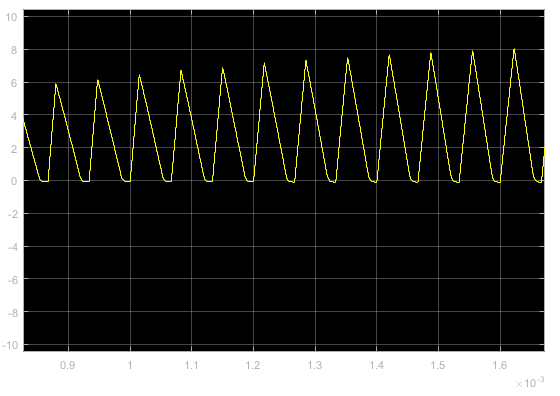
\includegraphics[width=0.82\textwidth]{sonuclar/onceki_tez_susturma_l1_yakin.png}
  \caption{Nötr anahtar susturma benzetimindeki $L_1$ endüktör akımından büyütülmüş kesit (Senaryo~2).}
  \label{fig:susturma-l1-yakin}
\end{figure}

Senaryo~2'nin dört kanallı ekranı Şekil~\ref{fig:susturma-dort-kanal} altında verilmiştir; kanal sırası Senaryo~1 ile aynıdır. $L_1$ ve çıkış akımında görülen düşük frekanslı zarf bozulması, susturmanın tek başına oluşturduğu üçüncü harmonik artışıyla uyumludur.

\begin{figure}[H]
  \centering
  \includegraphics[width=0.98\textwidth]{../dosyalar/05_sonradan_gelenler/Senaryo_2/dalga_sekilleri_s2.jpg}
  \caption{Nötr anahtar susturma yönteminde filtre giriş gerilimi, filtrelenmiş gerilim, $L_1$ endüktör akımı ve LC filtre çıkış akımının birlikte gösterimi (Senaryo~2).}
  \label{fig:susturma-dort-kanal}
\end{figure}

Senaryo~2 FFT ekranlarında analiz tanımı Senaryo~1 ile aynıdır. Şekil~\ref{fig:susturma-l1-fft} altında $L_1$ akımının temel bileşeni \SI{3.396}{\ampere} ve THD değeri \%46,86; Şekil~\ref{fig:susturma-iout-fft} altında çıkış akımının temel bileşeni \SI{3.412}{\ampere} ve THD değeri \%46,35 olarak okunmaktadır. Filtre çıkışında THD'nin yüksek kalması, bozulmanın yalnız yüksek frekanslı anahtarlama dalgalanmasından değil, filtrenin geçiş bandına daha yakın düşük mertebeli harmoniklerden kaynaklandığını göstermektedir.

\begin{figure}[H]
  \centering
  \includegraphics[width=0.98\textwidth]{../dosyalar/05_sonradan_gelenler/Senaryo_2/THD_IL1.jpg}
  \caption{Nötr anahtar susturma yönteminde $L_1$ endüktör akımının FFT analizi: temel bileşen \SI{3.396}{\ampere}, $\mathrm{THD}_{L1}=\%46{,}86$ (Senaryo~2).}
  \label{fig:susturma-l1-fft}
\end{figure}

\begin{figure}[H]
  \centering
  \includegraphics[width=0.98\textwidth]{../dosyalar/05_sonradan_gelenler/Senaryo_2/THD_Iout.jpg}
  \caption{Nötr anahtar susturma yönteminde LC filtre çıkış akımının FFT analizi: temel bileşen \SI{3.412}{\ampere}, $\mathrm{THD}_{\mathrm{out}}=\%46{,}35$ (Senaryo~2).}
  \label{fig:susturma-iout-fft}
\end{figure}

Senaryo~3'ün ekranları Sin\textsuperscript{3} kompanzasyonunun sonuç setine ait olduğundan Bölüm~\ref{chap:sin3} altında ele alınmaktadır. Sayısal yorum yalnız görüntüden okunabilen kanallarla sınırlandırılmıştır; anahtarlama kaybı, yarı iletken sıcaklığı ve DA/AA güçleri kaydedilmediği için üç senaryo arasında doğrudan verim artışı yüzdesi hesaplanamaz.

\eksikistek{Verim ve güç adlandırma çelişkilerinin ham kayıtla çözümü}{Tablo~\ref{tab:onceki-benzetim-ozeti} içindeki verim yüzdelerinin DA giriş gücü, AA çıkış gücü, işaret yönü, analiz penceresi ve kayıp modeliyle ham kayıttan yeniden hesabını istiyoruz. Ayrıca 20~kVA, 25~kW ve yaklaşık 30~kW anma ifadelerinin hangi çalışma noktasına ait olduğunu gösteren ham tasarım belgesini istiyoruz. Bu kayıtlar gelmeden verim satırları tarihsel bulgu statüsünde kalacaktır.}

\section{Bölüm Sonucu}

T-tipi faz kolunun düşük güçte senkron buck benzeri davranışı, nötr kol üzerinden ters enerji dolaşımının fiziksel kaynağını açıklamaktadır. Klasik anahtarlama akım sürekliliği ve THD bakımından avantajlıyken ters akımın RMS ve iletim kayıplarını büyütmesine izin verebilir. Önerilen anahtarlama, ters akımı sürdüren nötr komutunu düşük güç bölgesinde bastırarak kayıp yolunu azaltmayı amaçlamakta; karşılığında süreksiz iletim ve üçüncü harmonik cezası oluşturmaktadır.

Üç benzetim senaryosu mekanizma sırasını desteklemektedir: nötr anahtar susturma çıkış THD değerini \%2,14'ten \%46,35'e yükseltirken Sin\textsuperscript{3} kompanzasyonu değeri \%7,79'a indirmiştir. Ham modelin bulunmaması kapı eşlemesini ve verim iddiasını sınırlandırmaktadır. Sonraki bölümde kompanzasyonun matematiksel tanımı, kapalı çevrim içindeki konumu, Bode analizi ve çalışma noktasına bağlı sonuçları ele alınmaktadır.

\chapter{SİN\texorpdfstring{\textsuperscript{3}}{3} TABANLI İLERİ BESLEME KOMPANZASYONU VE KAPALI ÇEVRİM ANALİZİ}
\label{chap:sin3}

Nötr anahtar susturma yöntemi ters akım dolaşımını azaltmayı hedeflerken akımı süreksiz iletime zorlamakta ve özellikle düşük mertebeli harmonikleri büyütmektedir. Bölüm~\ref{chap:anahtarlama} altındaki senaryo kayıtları, çıkış akımı THD değerinin klasik yöntemdeki \%2,14 düzeyinden susturma sonrasında \%46,35 düzeyine çıktığını; Sin\textsuperscript{3} kompanzasyonu eklendiğinde ise \%7,79'a gerilediğini göstermiştir. Bölümün amacı bu iyileşmenin arkasındaki matematiksel yapıyı kurmak, kompanzasyon katsayılarını doğru trigonometrik özdeşlikle ve doğrulanmış parametre setiyle yeniden hesaplamak ve kapalı çevrim ile kararlılık incelemesinin yöntemini vermektir.

\section{Sin\texorpdfstring{\textsuperscript{3}}{3} Bileşeninin Matematiksel Tanımı}

Zaman $t$, şebeke temel açısal frekansı $\omega_0$, PLL faz başlangıcı/ofseti $\phi$ ve boyutsuz elektriksel açı $\theta=\omega_0t+\phi$ ile gösterilsin. Kullanılan trigonometrik özdeşlik
\begin{equation}
  \sin^3\theta=\frac{3}{4}\sin\theta-\frac{1}{4}\sin(3\theta)
  \label{eq:sin3-acilimi}
\end{equation}
biçimindedir. Eşitlik~\eqref{eq:sin3-acilimi} uyarınca $\sin^3\theta$ terimi yalnız üçüncü harmonikten oluşmaz; temel bileşen ile ters işaretli üçüncü harmonik bileşenini sabit bir oranla birlikte taşır. Boyutsuz Sin\textsuperscript{3} ileri besleme komutu $u_{\mathrm{ff},\sin^3}(\theta)$, temel bileşen kazanç katsayısı $K_1$ ve küp teriminin kazanç katsayısı $K_3$ ile
\begin{equation}
  u_{\mathrm{ff},\sin^3}(\theta)=K_1\sin\theta+K_3\sin^3\theta
  \label{eq:sin3-genel-komut}
\end{equation}
olarak tanımlandığında Eşitlik~\eqref{eq:sin3-acilimi} kullanılarak
\begin{equation}
  u_{\mathrm{ff},\sin^3}(\theta)
  =\left(K_1+\frac{3K_3}{4}\right)\sin\theta-\frac{K_3}{4}\sin(3\theta)
  =A_1\sin\theta+A_3\sin(3\theta)
  \label{eq:sin3-esdeger-katsayilar}
\end{equation}
elde edilir. Eşitlik~\eqref{eq:sin3-genel-komut} ile Eşitlik~\eqref{eq:sin3-esdeger-katsayilar} arasındaki dönüşümde $A_1=K_1+3K_3/4$ temel sinüs katsayısını, $A_3=-K_3/4$ ise doğrudan üçüncü harmonik katsayısını gösterir. Yazılımda doğrudan $\sin(3\theta)$ kullanılması ile $\sin^3\theta$ kullanılması aynı işlem değildir; gerçek uygulama kodu geldiğinde kullanılan gösterim, katsayı ve işaret Eşitlik~\eqref{eq:sin3-esdeger-katsayilar} üzerinden kilitlenecektir.

\section{Basitleştirilmiş Türetimlerin Geçerlilik Sınırı}

Kompanzasyon katsayılarının tek bir cebirsel iptal koşulundan (örneğin sabit bir $K_1/K_3$ oranından) türetilmesi cazip görünse de anahtarlamalı dönüştürücüde geçerli değildir. Bunun üç nedeni vardır. Birincisi, belirli bir çalışma noktasında gözlenen temel ve üçüncü harmonik genliklerinin oranı, girişten bağımsız bir sistem transfer fonksiyonu değildir; yalnız o dalga biçimini ve o çalışma noktasını tarif eder. İkincisi, anahtarlamalı, doğrusal olmayan veya periyodik zamanla değişen bir sistemde süperpozisyon kanıtlanmadan uygulanamaz; giriş dalga biçimi değiştirildiğinde aynı skaler oranın yeniden kullanılması örtük bir doğrusallık varsayımıdır. Üçüncüsü, komutun frekans içeriği ile dönüştürücünün çıkış akımı aynı büyüklük değildir; çıkıştaki harmonik iptal koşulu, bitki dinamiği ve harmonikler arası bağlaşım bilinmeden yalnız trigonometrik özdeşlikten çıkarılamaz.

Periyodik zamanla değişen sistemin doğru genel çerçevesi harmonik transfer fonksiyonudur. Kesilmiş harmonik giriş ve çıkış vektörleri $\mathbf{U}(s)$ ile $\mathbf{I}(s)$, harmonik transfer matrisi $\mathbf{G}_{\mathrm{H}}(s)$, matrisin $(k,n)$ elemanı $G_{k,n}(s)$ ve kesme mertebesi $N_h$ ile gösterildiğinde
\begin{equation}
  \mathbf{I}(s)=\mathbf{G}_{\mathrm{H}}(s)\mathbf{U}(s),
  \qquad
  I_k(s)=\sum_{n=-N_h}^{N_h}G_{k,n}(s)U_n(s)
  \label{eq:htf-matris-iliskisi}
\end{equation}
yazılır \citep{Wereley1991,Liao2022}. Eşitlik~\eqref{eq:htf-matris-iliskisi}, tek bir giriş harmoniğinin birden fazla çıkış harmoniğine bağlaşabileceğini gösterir. Geçerli bir HTF modeli için çalışma noktası, frekans taraması, $N_h$ ve kesme hatası birlikte belirtilmelidir. Kompanzasyon katsayıları bu çerçevede ya periyodik çalışma noktası çevresinde doğrusallaştırılmış model üzerinden ya da küçük işaretli temel ve üçüncü harmonik enjeksiyon ölçümleriyle belirlenmelidir; katsayıların çalışma noktasına bağlılığı Kesim~\ref{sec:sin3-yeniden-tarama} altında sayısal olarak da gösterilmektedir.

Kompanzasyonun hedefi, akımın ölçülen üçüncü harmonik fazına ters yönde bir modülasyon bileşeni üretirken temel akım genliğini korumaktır. Uygulama kazancı yalnız THD eniyilemesiyle seçilmemeli; modülasyon doygunluğu, DA bara kullanımı, akım RMS değeri, kontrol eforu ve düşük güçten orta güce geçişte süreklilik koşulları birlikte değerlendirilmelidir. Üçüncü harmonik enjeksiyonunun modülasyon kullanımını değiştirebildiği bilinse de buradaki amaç klasik üçüncü harmonik PWM ile DA bara kullanımını artırmak değil, nötr susturmanın oluşturduğu akım zarfı bozulmasını azaltmaktır \citep{Holmes2003}.

\eksikistek{Gerçek Sin\textsuperscript{3} kodu ve harmonik bağlaşım ölçümü}{(1) Uygulamadaki ileri besleme ifadesinin $K_1\sin\theta+K_3\sin^3\theta$ mı yoksa $K_1\sin\theta+K_3\sin(3\theta)$ mı olduğunu; işaret, normalizasyon, birim, doyum ve etkinleştirme koşullarıyla birlikte gösteren kaynak kodu istiyoruz (istek listesi R07). (2) Temel ve üçüncü harmonik giriş--çıkış bağlaşımını belirlemek için model doğrusallaştırması veya küçük işaretli harmonik enjeksiyon taraması istiyoruz; Eşitlik~\eqref{eq:htf-matris-iliskisi} bu veriler olmadan sayısallaştırılamaz.}

\section{Düşük Güçte Harmonik Oluşum Mekanizması}

Şekil~\ref{fig:senkron-buck-esdeger} altında verilen iki-buck eşdeğeri, pozitif ve negatif alternansların aynı fiziksel mekanizmayla incelenmesini sağlar. Pozitif alternansta etkin yarım bara gerilimi $V_h$, anık şebeke gerilimi $v_g(\theta)>0$, anahtarlama periyodu $T_s$, boyutsuz görev oranı $d(\theta)\in[0,1]$ ve eşdeğer endüktans $L$ olarak tanımlansın. İdeal anahtarlama-periyodu modeli ve periyot boyunca yaklaşık sabit gerilim kabulü altında anahtar iletim süresindeki akım tepe değeri $I_{\mathrm{pk}}(\theta)$
\begin{equation}
  I_{\mathrm{pk}}(\theta)=\frac{V_h-v_g(\theta)}{L}\,d(\theta)T_s
  \label{eq:dcm-tepe-akimi}
\end{equation}
olur. Eşitlik~\eqref{eq:dcm-tepe-akimi}, iletim başlangıcında akımın sıfır olduğu DCM darbesi içindir. Anahtar kesime girdiğinde akım $-v_g/L$ eğimiyle sıfıra düşerse, gerçek boşalma süresinin $T_s$'ye oranı olan boyutsuz $\delta(\theta)$
\begin{equation}
  \delta(\theta)=\left(\frac{V_h}{v_g(\theta)}-1\right)d(\theta)
  \label{eq:dcm-bosalma-suresi}
\end{equation}
olarak bulunur. Eşitlik~\eqref{eq:dcm-bosalma-suresi}, yalnızca $v_g(\theta)>0$ ve akımın aynı periyotta sıfıra ulaştığı aralıkta geçerlidir. Üçgensel akım darbesinin bir anahtarlama periyodundaki ortalaması $\bar i_L(\theta)$
\begin{equation}
  \bar i_L(\theta)=\frac{1}{2}I_{\mathrm{pk}}(\theta)\,[d(\theta)+\delta(\theta)]
  =\frac{T_sV_h}{2L}\frac{V_h-v_g(\theta)}{v_g(\theta)}d^2(\theta)
  \label{eq:dcm-ortalama-akim}
\end{equation}
ifadesini verir \citep{Erickson2001,Chen2010}. Eşitlik~\eqref{eq:dcm-ortalama-akim}, Eşitlik~\eqref{eq:dcm-tepe-akimi} ile Eşitlik~\eqref{eq:dcm-bosalma-suresi} kullanılarak üçgen alanından elde edilmiştir. Sinüzoidal görev oranının tepe katsayısı $d_m$ ve şebeke geriliminin tepe değeri $V_m$ olmak üzere $d(\theta)=d_m\sin\theta$ ve $v_g(\theta)=V_m\sin\theta$ kabulü altında pozitif alternans zarfı
\begin{equation}
  \bar i_L(\theta)=\frac{T_sV_hd_m^2}{2LV_m}\sin\theta\,[V_h-V_m\sin\theta],
  \qquad 0<\theta<\pi
  \label{eq:dcm-sinus-zarfi}
\end{equation}
biçimine dönüşür. Eşitlik~\eqref{eq:dcm-sinus-zarfi}, görev oranı sinüzoidal olsa bile ortalama akımın saf sinüs kalmadığını doğrudan göstermektedir: zarf, $\sin\theta$ ile $[V_h-V_m\sin\theta]$ çarpımından oluştuğu için sıfır geçişlerinde sinüsten hızlı yükselir ve alternans ortasında çöker. Düşük güçte çalışma noktasına bağlı akım harmoniklerinin büyüyebildiği, saha ölçümü ile zamanla değişen modeller üzerinden de raporlanmıştır \citep{Chicco2009,Du2013}.

DCM koşulu darbenin aynı anahtarlama periyodunda sona ermesini gerektirir:
\begin{equation}
  d(\theta)+\delta(\theta)\leq 1
  \quad\Longrightarrow\quad
  d(\theta)\leq d_{\mathrm{krit}}(\theta)=\frac{v_g(\theta)}{V_h}.
  \label{eq:dcm-kritik-gorev}
\end{equation}
Eşitlik~\eqref{eq:dcm-kritik-gorev} içindeki kritik görev oranı faz açısına ve gerilim oranına bağlıdır; tek bir evrensel sayı değildir. Doğrulanmış parametre setinde ($V_h=\SI{215.75}{\volt}$, $V_m=\SI{169.4}{\volt}$) tepe değeri $V_m/V_h\simeq0{,}785$'tir ve Kesim~\ref{sec:sin3-yeniden-tarama} altındaki sayısal tarama, $d_m$ bu sınırı aştığında alternans ortasında CCM'ye geçildiğini doğrulamaktadır. Sıfır geçişte $v_g\rightarrow0$ olduğundan ideal ifadenin tek başına kullanılması uygun değildir; ölü zaman, minimum darbe ve sonlu akım eşiği ayrıca uygulanmalıdır.

DCM zarfı ile sürekli iletim modeli ortak bir görev oranı üzerinden birleştirilebilir. Temel ve üçüncü harmonik görev katsayıları $D_1$ ve $D_3$ kullanılarak
\begin{equation}
  d(\theta)=D_1\sin\theta+D_3\sin^3\theta
  \label{eq:ccm-gorev-harmonik}
\end{equation}
yazılsın; Eşitlik~\eqref{eq:ccm-gorev-harmonik} içindeki $D_1$ ve $D_3$, Eşitlik~\eqref{eq:sin3-esdeger-katsayilar} altındaki $K_1$ ile $K_3$'e uygulama ölçeklemesi sonrası karşılık gelen görev katsayılarıdır. Pozitif alternansta kayıpsız CCM ortalama diferansiyel denklemi
\begin{equation}
  L\frac{\mathrm{d}\bar i_{L,\mathrm{CCM}}}{\mathrm{d}t}
  =V_h d(\theta)-V_m\sin\theta
  \label{eq:ccm-diferansiyel}
\end{equation}
biçimindedir \citep{Erickson2001,Mohan2003}. Eşitlik~\eqref{eq:ccm-diferansiyel}, $\theta=\omega_0t+\phi$ bağı ve Eşitlik~\eqref{eq:ccm-gorev-harmonik} kullanılarak integre edildiğinde
\begin{equation}
  \bar i_{L,\mathrm{CCM}}(\theta)
  = I_0+\frac{V_m-V_hD_1}{\omega_0L}\cos\theta
  -\frac{V_hD_3}{3\omega_0L}\cos(3\theta)
  \label{eq:ccm-akim-cozumu}
\end{equation}
elde edilir; burada $\sin^3\theta$ önce Eşitlik~\eqref{eq:sin3-acilimi} ile harmonik bileşenlerine ayrılmıştır ve $I_0$, DCM--CCM geçişinde akım sürekliliğinden belirlenen integrasyon sabitidir. Anahtarlama-periyodu ortalama akımının parçalı modeli
\begin{equation}
  \bar i_L(\theta)=
  \begin{cases}
    \bar i_{L,\mathrm{DCM}}(\theta), & d(\theta)<d_{\mathrm{krit}}(\theta),\\
    \bar i_{L,\mathrm{CCM}}(\theta), & d(\theta)\geq d_{\mathrm{krit}}(\theta)
  \end{cases}
  \label{eq:dcm-ccm-parcali-model}
\end{equation}
ile ifade edilir. Tam periyot şebeke akımı $i_g(\theta)$ yarım dalga tek simetrisine sahipse $n$'inci sinüs Fourier katsayısı
\begin{equation}
  B_n=\frac{1}{\pi}\int_0^{2\pi}i_g(\theta)\sin(n\theta)\,\mathrm{d}\theta,
  \qquad n=1,2,\ldots
  \label{eq:akim-fourier-katsayisi}
\end{equation}
olarak hesaplanır \citep{Oppenheim1997}. Eşitlik~\eqref{eq:akim-fourier-katsayisi} içindeki $B_1$ ve $B_3$ sırasıyla temel ve üçüncü harmonik sinüs katsayılarını verir; yarım dalga simetrisi sağlanmazsa DA ve kosinüs katsayıları da ayrıca hesaplanmalıdır.

\section{Katsayıların Doğru Özdeşlikle Yeniden Hesabı}
\label{sec:sin3-yeniden-tarama}

Eşitlik~\eqref{eq:dcm-tepe-akimi}--\eqref{eq:dcm-ccm-parcali-model} ile kurulan parçalı model, kompanzasyon katsayılarının sayısal olarak taranmasına olanak tanır. Tarama 01.09.2026 tarihli MATLAB koşusuyla, doğrulanmış parametre seti ($V_{\mathrm{dc}}=\SI{431.5}{\volt}$, $V_h=\SI{215.75}{\volt}$, $V_m=\SI{169.4}{\volt}$, $f_0=\SI{50}{\hertz}$, $f_s=\SI{10}{\kilo\hertz}$, $L=L_1=\SI{600}{\micro\henry}$) üzerinde yapılmıştır. Model, nötr anahtarı susturulmuş faz kolunu anahtarlama periyodu bazında parçalı doğrusal çözmekte; susturma nedeniyle akım tabanı sıfırda kesilmekte ve DCM--CCM geçişleri periyotlar arası başlangıç akımıyla doğal olarak oluşmaktadır. Kanıt sınırı açıktır: bu, Tablo~\ref{tab:model-katmanlari} içindeki analitik/ortalama katmandır; ölü zaman, denetleyici, $C_f$--$L_2$ dinamiği ve kayıplar içermez, verim sonucu üretmez.

Üç bulgu öne çıkmaktadır. Birincisi, saf sinüzoidal görev oranıyla ($D_3=0$) süreksiz iletimdeki üçüncü harmonik oranı $d_m=0{,}1$--$0{,}7$ aralığında sabit \%39,96 çıkmaktadır; Tablo~\ref{tab:dcm-saf-sinus-harmonikleri} bu taramayı vermektedir. Oranın $d_m$'den bağımsızlığı, Eşitlik~\eqref{eq:dcm-sinus-zarfi} zarfının şeklinin $d_m^2$ ölçeklemesinden bağımsız olmasının doğrudan sonucudur. $d_m=0{,}8$ satırında oran değişmekte ve akım hızla büyümektedir; bu, $d_{\mathrm{krit}}$ tepe değerinin ($\simeq0{,}785$) aşılıp alternans ortasında CCM'ye geçilmesinin göstergesidir ve ideal tam-DCM modelinin geçerlilik sınırını işaretler.

\begin{table}[htbp]
  \centering
  \caption{Saf sinüzoidal görev oranı için parçalı DCM/CCM modelinden hesaplanan harmonik genlikler (01.09.2026 koşusu).}
  \label{tab:dcm-saf-sinus-harmonikleri}
  \small
  \begin{tabular}{S[table-format=1.1] S[table-format=1.4] S[table-format=1.4] S[table-format=1.4] S[table-format=1.4] S[table-format=2.2]}
    \toprule
    {$d_m$} & {$I_1$ (A)} & {$I_3$ (A)} & {$I_5$ (A)} & {$I_7$ (A)} & {$100I_3/I_1$} \\
    \midrule
    0.1 & 0.0764 & 0.0305 & 0.0044 & 0.0015 & 39.96 \\
    0.2 & 0.3055 & 0.1221 & 0.0174 & 0.0058 & 39.96 \\
    0.3 & 0.6874 & 0.2747 & 0.0392 & 0.0131 & 39.96 \\
    0.4 & 1.2220 & 0.4884 & 0.0698 & 0.0233 & 39.96 \\
    0.5 & 1.9093 & 0.7631 & 0.1090 & 0.0363 & 39.96 \\
    0.6 & 2.7494 & 1.0988 & 0.1570 & 0.0523 & 39.96 \\
    0.7 & 3.7423 & 1.4956 & 0.2137 & 0.0712 & 39.96 \\
    \bottomrule
  \end{tabular}
\end{table}

İkincisi, önceki katsayı taramalarında öne çıkan aday çiftler doğrulanmış parametre setine taşınamamaktadır. $(D_1,D_3)$ için $(0{,}45,\ 0{,}37)$, $(0{,}44,\ 0{,}38)$ ve $(0{,}41,\ 0{,}41)$ noktaları bu sette $I_1\simeq8{,}5$--\SI{9.2}{\ampere} temel akım (gerçek düşük güç çalışma noktasının yaklaşık dört katı), $I_3/I_1\simeq\%50$ ve $\mathrm{THD}\simeq\%68$ üretmektedir. Aynı adayların daha önce \%1--2 düzeyinde üçüncü harmonik oranıyla raporlanmış olması çelişki değildir; katsayıların gerilim oranına, endüktansa ve akım seviyesine bağlı olduğunu, tek bir $(D_1,D_3)$ çiftinin bütün çalışma noktalarına genellenemeyeceğini gösterir. Bulgu, üç fazlı fiziksel modeldeki bağımsız yeniden koşunun (Kesim~\ref{sec:sin3-guc-karsilastirma}) tarihsel THD iyileşmesini üretememesiyle de tutarlıdır.

Üçüncüsü, aynı tarama gerçek düşük güç çalışma noktası için düzeltilmiş bir aday vermektedir. $I_{\mathrm{rms}}$ değeri deney kayıtlarındaki \SI{2.26}{\ampere} düzeyiyle uyumlu ($2{,}0$--\SI{2.6}{\ampere}) tutulup görev oranı kırpılması dışlandığında en iyi nokta
\begin{equation}
  (D_1, D_3)=(0{,}34,\ 0{,}40)
  \;\Longrightarrow\;
  \frac{I_3}{I_1}=\%0{,}15,\quad \mathrm{THD}=\%4{,}72,\quad I_{\mathrm{rms}}=\SI{2.02}{\ampere},\quad d_{\max}=0{,}74
  \label{eq:sin3-duzeltilmis-optimum}
\end{equation}
olarak bulunmuştur; Eşitlik~\eqref{eq:sin3-esdeger-katsayilar} ile doğrudan-harmonik eşdeğeri $(A_1,A_3)=(0{,}64,\ -0{,}10)$'dur. Şekil~\ref{fig:sin3-yeniden-tarama}, katsayı düzlemindeki üçüncü harmonik oranını, uygun akım bölgesini ve en iyi noktadaki akım zarfının saf sinüs görev oranına göre düzelmesini birlikte göstermektedir. Kompanzasyonlu zarfta kalan \%4,7'lik THD, ağırlıkla beşinci ve yedinci harmoniklerden gelmektedir; Sin\textsuperscript{3} terimi yapısı gereği yalnız temel ve üçüncü harmoniği şekillendirdiğinden bu kalıntı, yöntemin yapısal sınırıdır.

\begin{figure}[htbp]
  \centering
  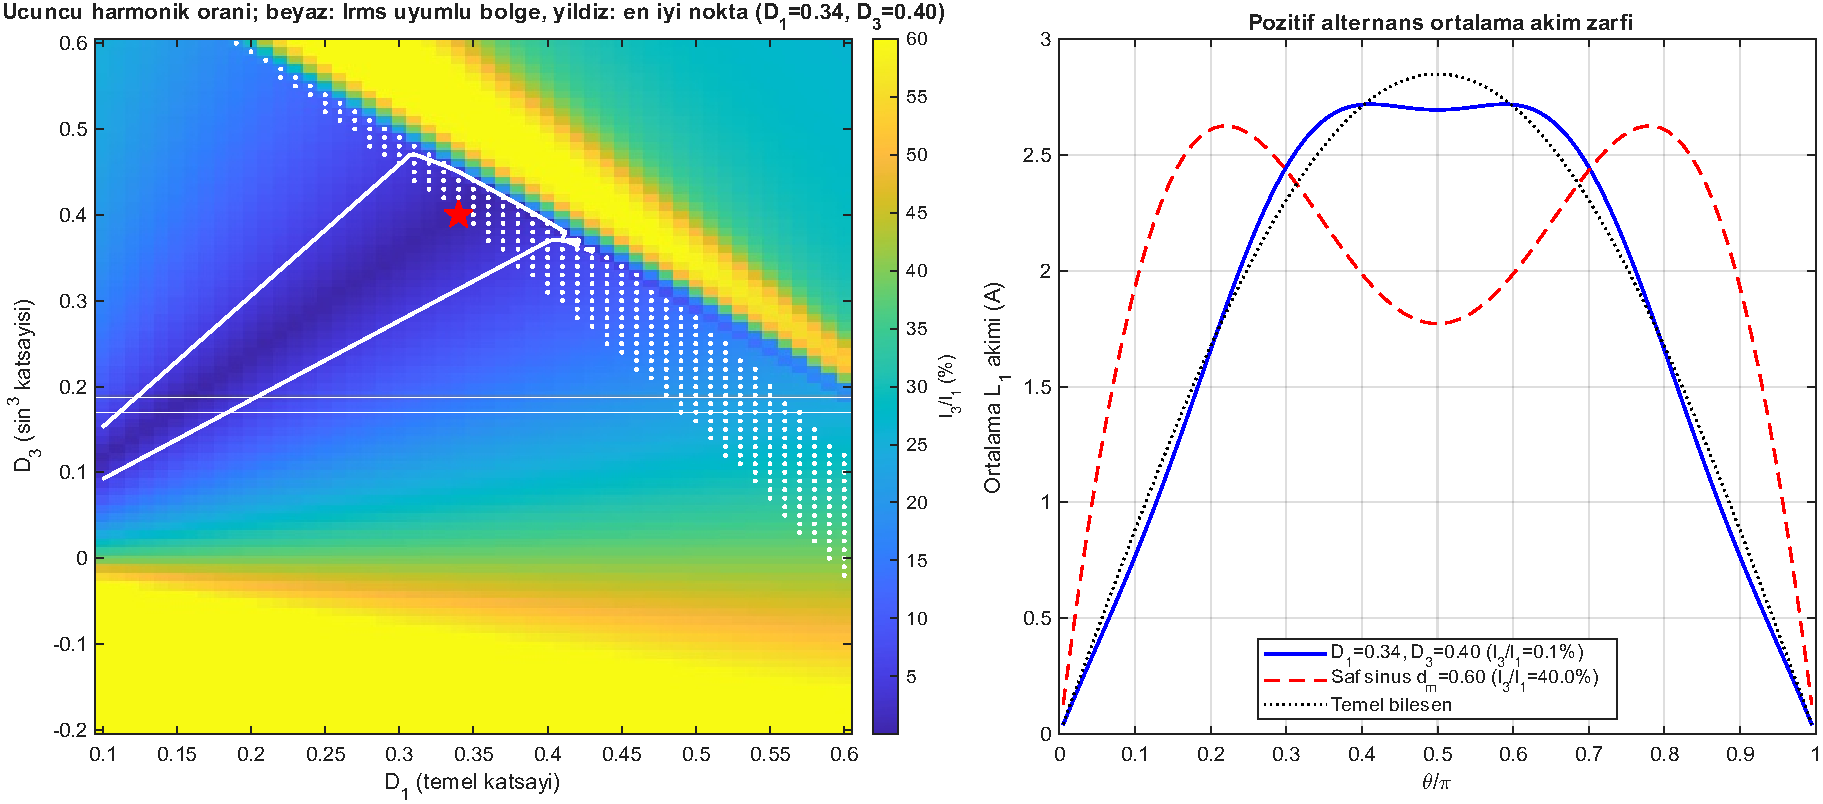
\includegraphics[width=\textwidth]{../tez-matlab-simulink/results/sin3_rescan_20260901/sin3_katsayi_taramasi_20260901.pdf}
  \caption{$(D_1,D_3)$ katsayı düzleminde üçüncü harmonik oranı (sol; beyaz noktalar \SI{2.0}{}--\SI{2.6}{\ampere} RMS bölgesini, yıldız en iyi noktayı gösterir) ve en iyi nokta ile saf sinüs görev oranının ortalama akım zarfı karşılaştırması (sağ). Parçalı DCM/CCM analitik modeli, 01.09.2026 koşusu.}
  \label{fig:sin3-yeniden-tarama}
\end{figure}

Eşitlik~\eqref{eq:sin3-duzeltilmis-optimum} ile verilen çift, uygulanacak nihai kazanç değil, doğrulanmış parametre setiyle tutarlı ilk analitik adaydır. Nihai seçim; gerçek koddaki gösterim (Eşitlik~\eqref{eq:sin3-esdeger-katsayilar} ayrımı), anahtarlamalı model, ölü zaman ve kapalı çevrim etkileşimi doğrulandıktan sonra yapılacaktır.

\section{Önerilen Yapı ve İleri Besleme Mekanizması}

İleri besleme yolunun fiziksel işlevi, evirici tarafındaki eşdeğer kaynak gerilimini şebeke gerilimine yaklaştırmaktır. PLL şebekeye kilitlendikten sonra, akım komutu uygulanmadan önce, evirici çıkışı ile şebeke eşpotansiyel ise seri $Z_1+Z_2$ filtre ve şebeke empedansından akan akım sıfıra yaklaşır; Şekil~\ref{fig:eski-feedforward-etkisi} bu durumu eşdeğer kaynaklar üzerinde, Şekil~\ref{fig:eski-espotansiyel-dalga} ise gerilim dalga biçimleri ve sıfır akım kaydıyla göstermektedir. Akım referansı uygulandığında denetleyicinin üretmesi gereken ek gerilim yalnız empedans düşümünü karşılayacak küçük bir bileşendir; akım küçüldükçe bu bileşen mutlak olarak küçülür ve modeldeki küçük gerilim hataları göreli olarak daha görünür hâle gelir. İleri besleme teriminin düşük akımdaki göreli önemi bu mekanizmadan kaynaklanır.

\begin{figure}[htbp]
  \centering
  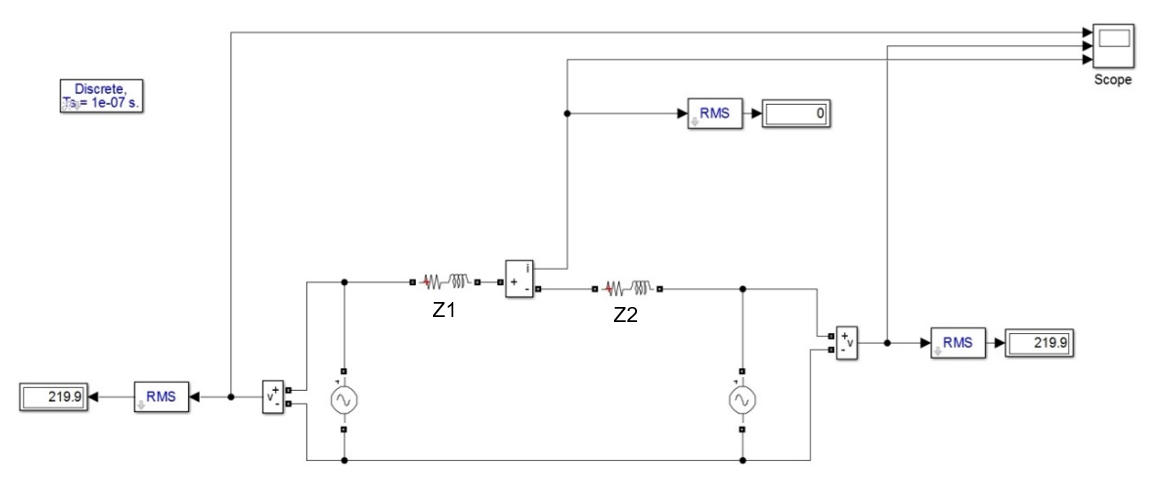
\includegraphics[width=0.96\textwidth]{sonuclar/eski_sekil_4_18_feedforward_etkisi.png}
  \caption{İleri besleme bileşeninin eşdeğer kaynaklar ve seri empedanslar üzerindeki etkisini gösteren benzetim modeli.}
  \label{fig:eski-feedforward-etkisi}
\end{figure}

\begin{figure}[htbp]
  \centering
  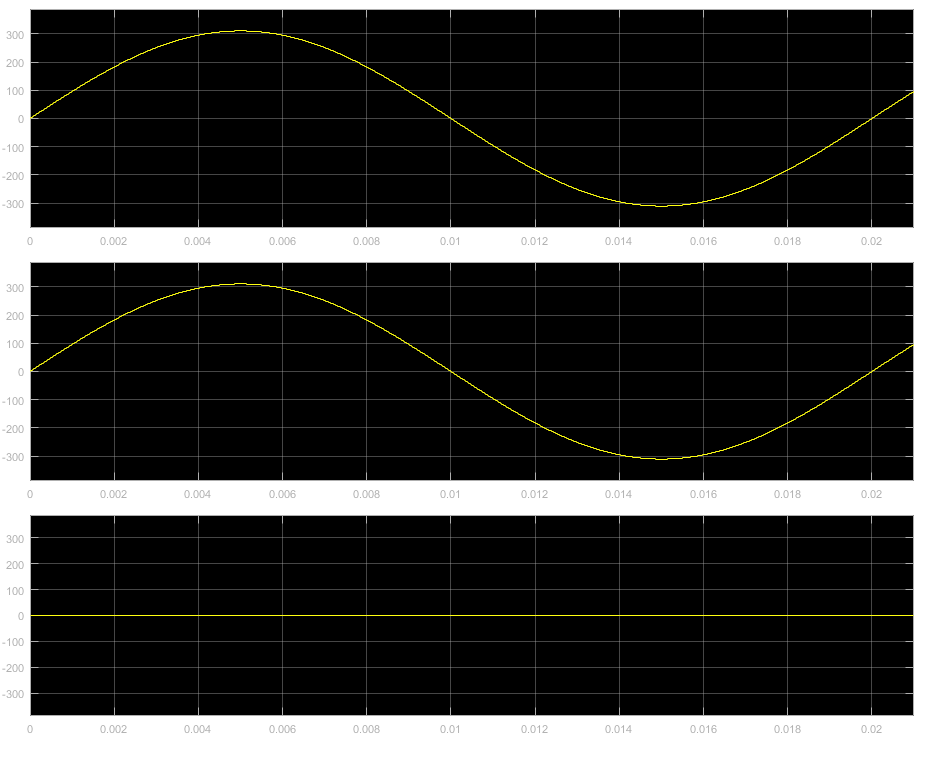
\includegraphics[width=0.90\textwidth]{sonuclar/eski_sekil_4_19_espotansiyel_dalga.png}
  \caption{Eşpotansiyel kaynakların gerilim dalga biçimleri ve kaynaklar arasındaki akımın sıfır oluşu. Kayıt, akım komutu öncesi başlangıç durumunu gösterir; kapalı çevrim izleme performansını kanıtlamaz.}
  \label{fig:eski-espotansiyel-dalga}
\end{figure}

Denetleyici devre dışı bırakılıp yalnız ileri besleme katsayısının değiştirildiği benzetim koşulu, yöntemin açık çevrim mekanizmasını ayırmak için yararlıdır; ancak kapalı çevrim performansı veya kararlılık kanıtı değildir. Şebeke gerilimi ileri beslemesi ideal durumda evirici ile şebeke gerilimini yaklaştırarak düşük akımdaki göreli gerilim hatasını azaltabilir; LCL filtre, ortak bağlantı noktası ölçümü ve dijital gecikme eklendiğinde aynı yol sanal empedans ve aktif sönümleme etkisi de oluşturabilir \citep{Lu2016}. İleri besleme yolunun etkisi bu nedenle yalnız gerilim düşümü hesabıyla sınırlandırılmamıştır. Güncel işlevsel zincir Şekil~\ref{fig:denetim-modulasyon-blok} üzerinde verilmiştir: Sin\textsuperscript{3} yolu akım denetleyicisiyle seri değil, modülasyon toplamında paralel bir ileri besleme bileşenidir ve nötr anahtar susturma kararı PWM üretiminden sonra kapı mantığında uygulanır.

\section{Kapalı Çevrim Modeli}

Faz başına gerilimden akıma LCL bitkisi $G_{vi}(s)$ Bölüm~\ref{chap:sistem} içinde Eşitlik~\eqref{eq:lcl-aktarim} ile tanımlanmıştır. PR denetleyicisi $C_i(s)$ Eşitlik~\eqref{eq:pr-denetleyici}, normalize modülasyon komutunu evirici kutup gerilimine dönüştüren PWM eşdeğer kazancı $K_{\mathrm{pwm}}$ ve toplam hesaplama--örnekleme--PWM gecikmesi $G_d(s)$ ile gösterilsin. Boyutsuz açık çevrim kazanç fonksiyonu $L(s)$
\begin{equation}
  L(s)=C_i(s)K_{\mathrm{pwm}}G_d(s)G_{vi}(s)
  \label{eq:sin3-acik-cevrim}
\end{equation}
olarak yazılır. Eşitlik~\eqref{eq:sin3-acik-cevrim} içindeki çarpanlar aynı işaret yönü ve birim sistemiyle kurulmalıdır. Toplam gecikme süresi $T_d$ olmak üzere sürekli-zaman yaklaşımında $G_d(s)=\exp(-sT_d)$ kullanılabilir; rasyonel Bode hesabında ise mertebesi belirtilmiş Padé yaklaşımı uygulanır. PR yapısının temel frekansta yüksek kazanç sağlaması sinüzoidal izleme hatasını azaltırken LCL rezonansı ek sönümleme veya uygun aktif sönümleme tasarımı gerektirir \citep{Teodorescu2006PR,Zhang2014PR}.

Referans izleme ve bozucu bastırma incelemesinde duyarlılık fonksiyonları
\begin{equation}
  S(s)=\frac{1}{1+L(s)},
  \qquad
  T(s)=\frac{L(s)}{1+L(s)}
  \label{eq:sin3-duyarlilik}
\end{equation}
biçimindedir. Eşitlik~\eqref{eq:sin3-duyarlilik} içindeki $S(s)$ duyarlılık, $T(s)$ tamamlayıcı duyarlılık fonksiyonudur. Doğrusal modelde toplama noktasına dışsal olarak eklenen $u_{\mathrm{ff},\sin^3}$ terimi Eşitlik~\eqref{eq:sin3-acik-cevrim} içindeki karakteristik paydayı tek başına değiştirmez. Gerçek uygulamada ise doygunluk, örnekleme, PLL faz hatası, anahtarlama kip değişimi ve ortak bağlantı noktası gerilimi üzerinden oluşan iç bağlaşım söz konusu ayrımı bozabilir. Şebeke gerilimi ileri beslemesinin dijital gecikmeyle birlikte LCL rezonansına sönümleme veya kararsızlaştırıcı etki verebilmesi literatürde hem model hem deneyle gösterilmiştir \citep{Lu2016,Wang2024}.

Şebeke akımı, akım referansı, Sin\textsuperscript{3} ileri besleme komutu ve şebeke geriliminin Laplace dönüşümleri sırasıyla $I_g(s)$, $I^{\ast}(s)$, $U_{\mathrm{ff},\sin^3}(s)$ ve $V_g(s)$ ile; şebeke geriliminden akıma bozucu aktarım $G_{vg}(s)$ ile gösterilsin. Harmonik kompanzasyonun doğrusal küçük işaret modeli, seçilen çalışma noktası çevresinde
\begin{equation}
  I_g(s)=T(s)I^{\ast}(s)+S(s)K_{\mathrm{pwm}}G_d(s)G_{vi}(s)U_{\mathrm{ff},\sin^3}(s)
  +S(s)G_{vg}(s)V_g(s)
  \label{eq:sin3-kapali-cevrim-girisleri}
\end{equation}
şeklinde ayrıştırılabilir; $G_{vg}(s)$'nin işareti seçilen gerilim ve akım yönlerine bağlıdır. Eşitlik~\eqref{eq:sin3-kapali-cevrim-girisleri}, Sin\textsuperscript{3} yolunun akım geri beslemesiyle seri bir denetleyici olmadığını, kapalı çevrim tarafından süzülen ayrı bir giriş olduğunu göstermektedir.

\section{Bode ve Kararlılık Marjı Analizi}

Kapalı çevrim incelemesi $L(s)$, $S(s)$ ve $T(s)$ fonksiyonlarının aynı fiziksel bitki, denetleyici ve gecikme modeliyle üretilmesine dayanır. Gerçek PR katsayıları, sönümleme ve gecikme henüz kilitlenmediğinden Şekil~\ref{fig:gecici-bode-lst} nihai kararlılık kanıtı değil, analiz zincirinin doğrulanmış filtre setiyle çalışan MATLAB çıktısıdır. Geçici parametrelerle elde edilen eğrilerin tezde tutulması yöntemi görünür kılmakta; sayısal marjların gerçek kod ve model geldiğinde aynı betikle değiştirilmesini sağlamaktadır.

\begin{figure}[htbp]
  \centering
  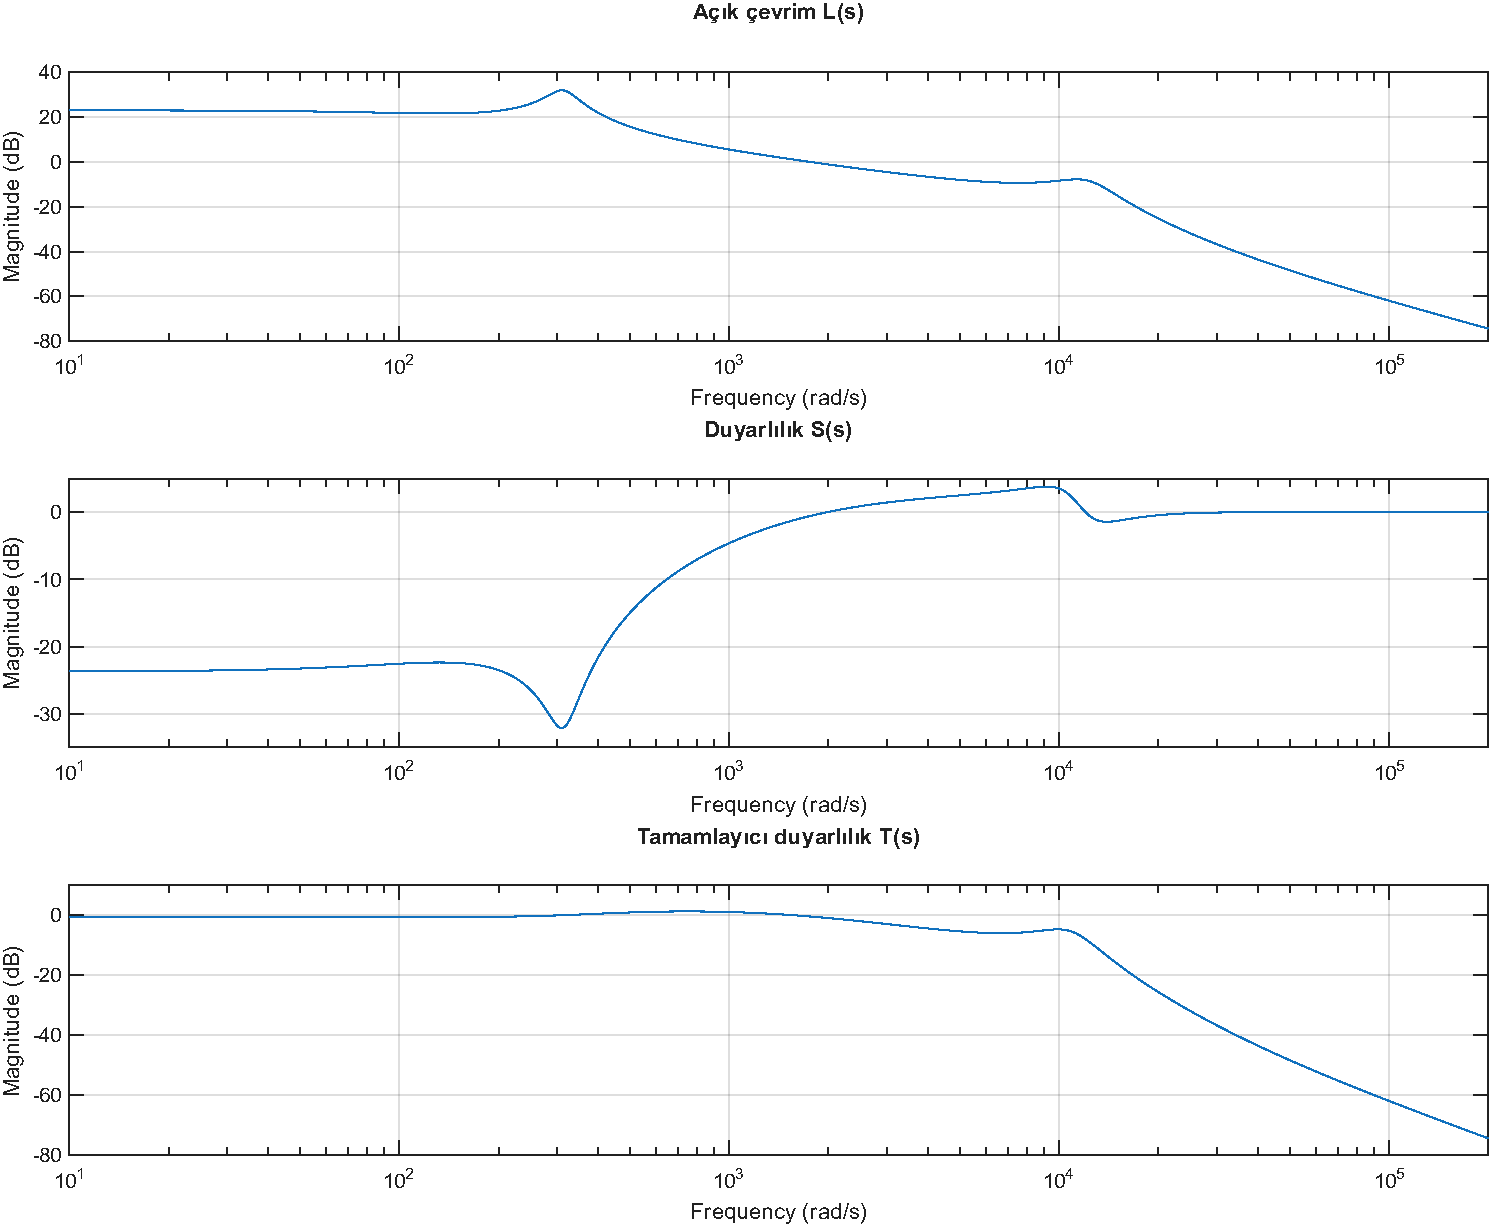
\includegraphics[width=0.96\textwidth]{../tez-matlab-simulink/results/stability/bode_LST.pdf}
  \caption{Geçici LCL--PR--gecikme modeli için MATLAB ile üretilen $L(s)$, $S(s)$ ve $T(s)$ büyüklük eğrileri; nihai parametre doğrulaması beklenmektedir.}
  \label{fig:gecici-bode-lst}
\end{figure}

Geçici modelde toplam gecikme \SI{150}{\micro\second} alınmış, kazanç marjı \SI{9.09}{\decibel} ve faz marjı $64{,}16^{\circ}$ hesaplanmıştır. Ek şebeke endüktansı $0$--\SI{2}{\milli\henry} arasında tarandığında aday model kararlı kalmış ve faz marjı $61{,}40^{\circ}$--$64{,}16^{\circ}$ aralığında değişmiştir. Sonuçlar analiz zincirinin çalıştığını gösterir; gerçek denetleyici katsayıları ve gecikme doğrulanmadan tezin nihai kararlılık marjı olarak savunulmayacaktır. Tablo~\ref{tab:sin3-kararlilik-kontrol-listesi}, incelemenin tamamlanma ölçütlerini ve mevcut durumu ayırmaktadır.

\begin{table}[htbp]
  \centering
  \caption{Kapalı çevrim kararlılık incelemesinin tamamlanma ölçütleri.}
  \label{tab:sin3-kararlilik-kontrol-listesi}
  \small
  \begin{tabularx}{\textwidth}{p{0.24\textwidth} X p{0.24\textwidth}}
    \toprule
    İnceleme & Değişkenler ve raporlanacak çıktı & Mevcut durum \\
    \midrule
    Nominal model & $L,S,T$, kesişim frekansları, kazanç/faz marjı & Geçici MATLAB çıktısı mevcut \\
    Şebeke dayanıklılığı & $R_g,L_g$ taraması ve en kötü marj & $L_g=0$--\SI{2}{\milli\henry} geçici taraması mevcut \\
    Sayısal gecikme & Örnekleme, hesaplama, PWM güncelleme ve ölçüm filtresi & Gerçek kodla doğrulanacak \\
    Çalışma noktası & Düşük, orta ve anma gücünde kip/doğrusallaştırma geçerliliği & Gerçek modelle doğrulanacak \\
    Doğrusal olmayan sınırlar & Modülasyon doyumu, akım sınırlama, nötr susturma geçişi & Zaman alanı testiyle doğrulanacak \\
    \bottomrule
  \end{tabularx}
\end{table}

Klasik doğrusal zamanla değişmeyen Bode incelemesi seçilen çalışma noktası çevresindeki yerel dinamiği verir. Nötr susturma periyodik kip değiştirdiği için harmonikler arası bağlaşım önemli hâle gelirse Eşitlik~\eqref{eq:htf-matris-iliskisi} çerçevesinde HTF veya harmonik durum uzayı modeli ayrıca kurulmalıdır; sonlu model için kesme mertebesi ve hata ölçütü raporlanmalıdır \citep{Liao2022}.

\eksikistek{Gerçek parametrelerle kararlılık doğrulaması}{Gerçek PR/PI katsayıları, örnekleme ve hesaplama gecikmeleri ile LCL sönümleme yöntemi geldiğinde $L$, $S$ ve $T$ eğrilerinin; kazanç/faz marjlarının ve $L_g$ taramasının düşük, orta ve anma gücü çalışma noktalarında yeniden üretilmesini istiyoruz. Nötr susturma kaynaklı kip değişimi anlamlıysa temel--üçüncü harmonik HTF matrisinin model doğrusallaştırması veya küçük işaret enjeksiyonuyla çıkarılmasını istiyoruz.}

\section{Düşük, Orta ve Nominal Güç Karşılaştırması}
\label{sec:sin3-guc-karsilastirma}

Senaryo~3 kayıtları, Sin\textsuperscript{3} kompanzasyonunun görsel kanıt zincirini tamamlamaktadır. Şekil~\ref{fig:sin3-l1-yakin} kompanzasyonlu $L_1$ akımının anahtarlama ölçeğindeki yapısını; Şekil~\ref{fig:sin3-dort-kanal} gerilim ve akım kanallarını ortak zaman ekseninde; Şekil~\ref{fig:sin3-l1-fft} ile Şekil~\ref{fig:sin3-iout-fft} iki akım ölçüm noktasındaki harmonik sonuçları göstermektedir.

\begin{figure}[H]
  \centering
  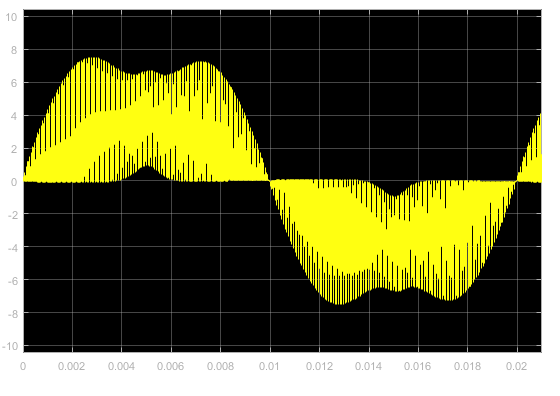
\includegraphics[width=0.82\textwidth]{sonuclar/eski_sekil_4_29_sin3_l1.png}
  \caption{Sin\textsuperscript{3} kompanzasyonlu nötr susturma benzetiminde $L_1$ akımının büyütülmüş görünümü (Senaryo~3).}
  \label{fig:sin3-l1-yakin}
\end{figure}

\begin{figure}[H]
  \centering
  \includegraphics[width=0.98\textwidth]{../dosyalar/05_sonradan_gelenler/Senaryo_3/dalga_sekilleri_s3.jpg}
  \caption{Sin\textsuperscript{3} kompanzasyonlu yöntemde filtre girişi gerilimi, filtrelenmiş gerilim, $L_1$ akımı ve çıkış akımı (Senaryo~3).}
  \label{fig:sin3-dort-kanal}
\end{figure}

Şekil~\ref{fig:sin3-dort-kanal} altında, susturma yönteminin Şekil~\ref{fig:susturma-dort-kanal} üzerindeki belirgin zarf bozulması kompanzasyon sonrasında azalmıştır; ancak çıkış akımı klasik yöntemdeki kadar sinüzoidal hâle gelmemiştir. Görsel karşılaştırma, aynı analiz penceresindeki FFT değerleriyle birlikte okunmalıdır.

\begin{figure}[H]
  \centering
  \includegraphics[width=0.98\textwidth]{../dosyalar/05_sonradan_gelenler/Senaryo_3/THD_IL1.jpg}
  \caption{Sin\textsuperscript{3} kompanzasyonlu yöntemde $L_1$ akımı FFT sonucu: temel bileşen \SI{3.752}{\ampere}, $\mathrm{THD}_{L1}=\%9{,}46$ (Senaryo~3).}
  \label{fig:sin3-l1-fft}
\end{figure}

\begin{figure}[H]
  \centering
  \includegraphics[width=0.98\textwidth]{../dosyalar/05_sonradan_gelenler/Senaryo_3/THD_Iout.jpg}
  \caption{Sin\textsuperscript{3} kompanzasyonlu yöntemde çıkış akımı FFT sonucu: temel bileşen \SI{3.766}{\ampere}, $\mathrm{THD}_{\mathrm{out}}=\%7{,}79$ (Senaryo~3).}
  \label{fig:sin3-iout-fft}
\end{figure}

Senaryo~3'te $L_1$ THD değeri susturma durumundaki \%46,86'dan \%9,46'ya, çıkış THD değeri ise \%46,35'ten \%7,79'a düşmüştür. İyileşme, Sin\textsuperscript{3} yolunun üçüncü harmonik cezasını önemli ölçüde azalttığını destekler. Klasik çıkış THD değerinin \%2,14 olması, kompanzasyonlu yöntemin harmonik bakımından klasik yöntemi geçmediğini de açıkça gösterir. Raporlanan \%93,70 verim değeri, ham kayıp modeli mevcut olmadığından yeniden doğrulanmış bir sonuç değildir.

Düşük, orta ve nominal güçte aynı denetim yapısının karşılaştırılması henüz tamamlanmış bir sonuç seti değildir; mevcut arşiv yalnız düşük güç kayıtlarını içermektedir. Tablo~\ref{tab:sin3-guc-karsilastirma-plani}, gelecek gerçek veri setinde doldurulacak ortak değerlendirme biçimini kilitlemektedir.

\begin{table}[htbp]
  \centering
  \caption{Sin\textsuperscript{3} kompanzasyonu için güç seviyesine bağlı ortak karşılaştırma tablosu.}
  \label{tab:sin3-guc-karsilastirma-plani}
  \small
  \begin{tabularx}{\textwidth}{p{0.14\textwidth} p{0.17\textwidth} X X}
    \toprule
    Güç bölgesi & Karşılaştırma kolları & Ölçülecek kararlı durum büyüklükleri & Geçici durum ve sınır kontrolleri \\
    \midrule
    Düşük & Klasik; susturma; susturma + Sin\textsuperscript{3} & Verim, $I_1$, THD, $I_3/I_1$, ters akım alanı, RMS akım & Kip geçişi, sıfır geçişi, minimum darbe, doyum \\
    Orta & Aynı üç kol & Aynı metrikler ve aynı FFT penceresi & Kompanzasyonun yumuşak azaltılması, akım basamağı \\
    Nominal & Klasik ve nihai öneri; güvenliyse üç kol & Verim, THD, sıcaklık, DA bara dengesi, güç faktörü & Akım sınırı, modülasyon doyumu, koruma ve toparlanma \\
    \bottomrule
  \end{tabularx}
\end{table}

\subsection{Bağımsız Yeniden Üretim Koşuları}

Eldeki dosya paketi Senaryo~1'e ait tek bir kaynak model ve Senaryo~1--3 için özet değerler içeren bir çalışma kitabı sağlamaktadır; Senaryo~2 ve Senaryo~3'e ait kaynak model ya da ham zaman serisi mevcut değildir. Senaryo~1 modeli R2023b ile kaydedilmiştir ve R2025b'de kaldırılan Specialized Power Systems ölçüm bloklarını içerdiği için değişmeden koşturulamamıştır. R2025b çalışma kopyasında $L_1$--$C_f$--$L_2$ değerleri \SI{600}{\micro\henry}--\SI{8}{\micro\farad}--\SI{200}{\micro\henry} yapılmış; dış IGBT'ler SKM100GB12T4, iç IGBT'ler IXYN100N65C3H1 ve yalnız harici iki diyot DSEI2x61-12B olarak eşlenmiştir.

Tablo~\ref{tab:r2025b-senaryo1-dogrulama}, çalışma kopyasıyla yapılan kademeli koşuları ayırmaktadır. Tam cihaz dinamikli \SI{1}{\milli\second} sağlık kontrolü başarıyla tamamlanmış, böylece blok eşlemesi ve elektriksel çözümün R2025b'de ilerlediği doğrulanmıştır. Aynı katmanda \SI{5}{\milli\second} koşu 1200~s duvar süresi içinde tamamlanmadığından hesap maliyeti sınırıyla sonlandırılmış, sayısal başarısızlık olarak etiketlenmemiştir. Cihaz dinamikleri sadeleştirilen \SI{25}{\milli\second} sistem koşusu ise \SI{21.3324}{\milli\second} anında diyot denklemlerinin yakınsamamasıyla durmuştur. Tam bir \SI{50}{\hertz} kararlı hâl penceresi ve geçerli THD/verim sonucu bu yüzden oluşmamıştır.

\begin{table}[htbp]
  \centering
  \caption{Seçilen LCL ve yarıiletken eşlemesiyle R2025b Senaryo~1 kademeli doğrulama koşuları.}
  \label{tab:r2025b-senaryo1-dogrulama}
  \footnotesize
  \begin{tabularx}{\textwidth}{>{\raggedright\arraybackslash}p{0.19\textwidth} >{\raggedright\arraybackslash}p{0.16\textwidth} >{\raggedright\arraybackslash}p{0.20\textwidth} >{\raggedright\arraybackslash}X}
    \toprule
    Koşu & Ufuk & Sonuç & Kanıt sınırı \\
    \midrule
    Seçilen filtre, sade sistem & \SI{5}{\milli\second} & Başarılı; son \%20 pencerede $I_{\mathrm{ac,rms}}=\SI{2.428}{\ampere}$ & Kısa süreli fiziksel tutarlılık; THD/verim değil. \\
    Seçilen filtre ve doğrulanmış cihazlar & \SI{1}{\milli\second} & Başarılı; 26,7~s hesap süresi & Cihaz/blok sağlık kontrolü; başlangıç geçicisi baskın. \\
    Aynı ayrıntılı cihaz katmanı & \SI{5}{\milli\second} & 1200~s içinde tamamlanmadı & Hesap maliyeti sınırı; performans sonucu yok. \\
    Seçilen filtre, sade sistem & \SI{25}{\milli\second} & \SI{21.3324}{\milli\second}'de yakınsama hatası & Kararlı hâl, THD ve verim geçersiz. \\
    \bottomrule
  \end{tabularx}
\end{table}

\SI{1}{\milli\second} koşuda ham DA bara gerilimi \SI{431.5}{\volt} olarak korunurken ideal gerilim kaynağının boş DA-link kapasitörlerini aniden şarj etmesi \SI{43.1}{\kilo\ampere} düzeyinde fiziksel olmayan bir başlangıç tepesi oluşturmuştur. Bu ilk koşul giderilmeden ve en az iki kararlı temel periyot tamamlanmadan ekrandaki anık güç, THD ve verim değerleri kullanılmamıştır; çalışma kitabında bildirilen \%92,5 verim ve yaklaşık \%15 THD, yeniden üretilmiş sonuç değil deney özeti olarak tutulmuştur.

Topoloji ve kapı mantığı bakımından bağımsız kontrol amacıyla, 12 IGBT'li üç fazlı Simscape modeli aynı koşullarda koşturulmuştur. Modelde klasik, nötr susturma ve susturma+$K_{\mathrm{sin3}}=-\SI{2}{\volt}$ kolları için geçersiz anahtarlama durumu sayısı sıfırdır; Tablo~\ref{tab:yeniden-uretim-fiziksel-s123} sonuçları vermektedir. Geçici model değerleri ($V_{\mathrm{dc}}=\SI{400}{\volt}$, $L_1=\SI{2}{\milli\henry}$, $L_2=\SI{1}{\milli\henry}$ ve \SI{2}{\micro\second} deneme ölü zamanı) kaynak modelle aynı olmadığından koşu bir parça-kayıp veya verim doğrulaması değildir.

\begin{table}[htbp]
  \centering
  \caption{Üç fazlı fiziksel model koşusu (22.08.2026); kaynak Senaryo~1--3'ün sayısal yeniden üretimi değil, kapı durumu ve yöntem yönelimi kontrolüdür.}
  \label{tab:yeniden-uretim-fiziksel-s123}
  \small
  \begin{tabularx}{\textwidth}{X r r r r}
    \toprule
    Yöntem & Faz RMS (A) & Ortalama THD (\%) & Nötr RMS (A) & Geçersiz durum \\
    \midrule
    Klasik & 2,227 & 10,898 & 0,639 & 0 \\
    Nötr susturma & 2,238 & 13,625 & 0,711 & 0 \\
    Susturma+Sin\textsuperscript{3} & 2,209 & 13,772 & 0,694 & 0 \\
    \bottomrule
  \end{tabularx}
\end{table}

Bu yeniden koşuda Sin\textsuperscript{3} terimi nötr RMS akımını yalnız susturmaya göre yaklaşık \%2,46 azaltmış, fakat faz THD'sini iyileştirmemiştir. Sonucun Senaryo~3 eğilimini yeniden üretmemesi bir başarısızlık gizleme nedeni değil, enjeksiyon noktası ile $K_1/K_3$ ölçeklerinin gerçek koddan kilitlenmesi gerektiğini gösteren negatif doğrulamadır; Kesim~\ref{sec:sin3-yeniden-tarama} altındaki katsayı taşınamazlığı bulgusuyla da tutarlıdır. Şekil~\ref{fig:yeniden-uretim-fiziksel-s123} kullanılan kazanç noktalarını ve iki metriği birlikte göstermektedir.

\begin{figure}[htbp]
  \centering
  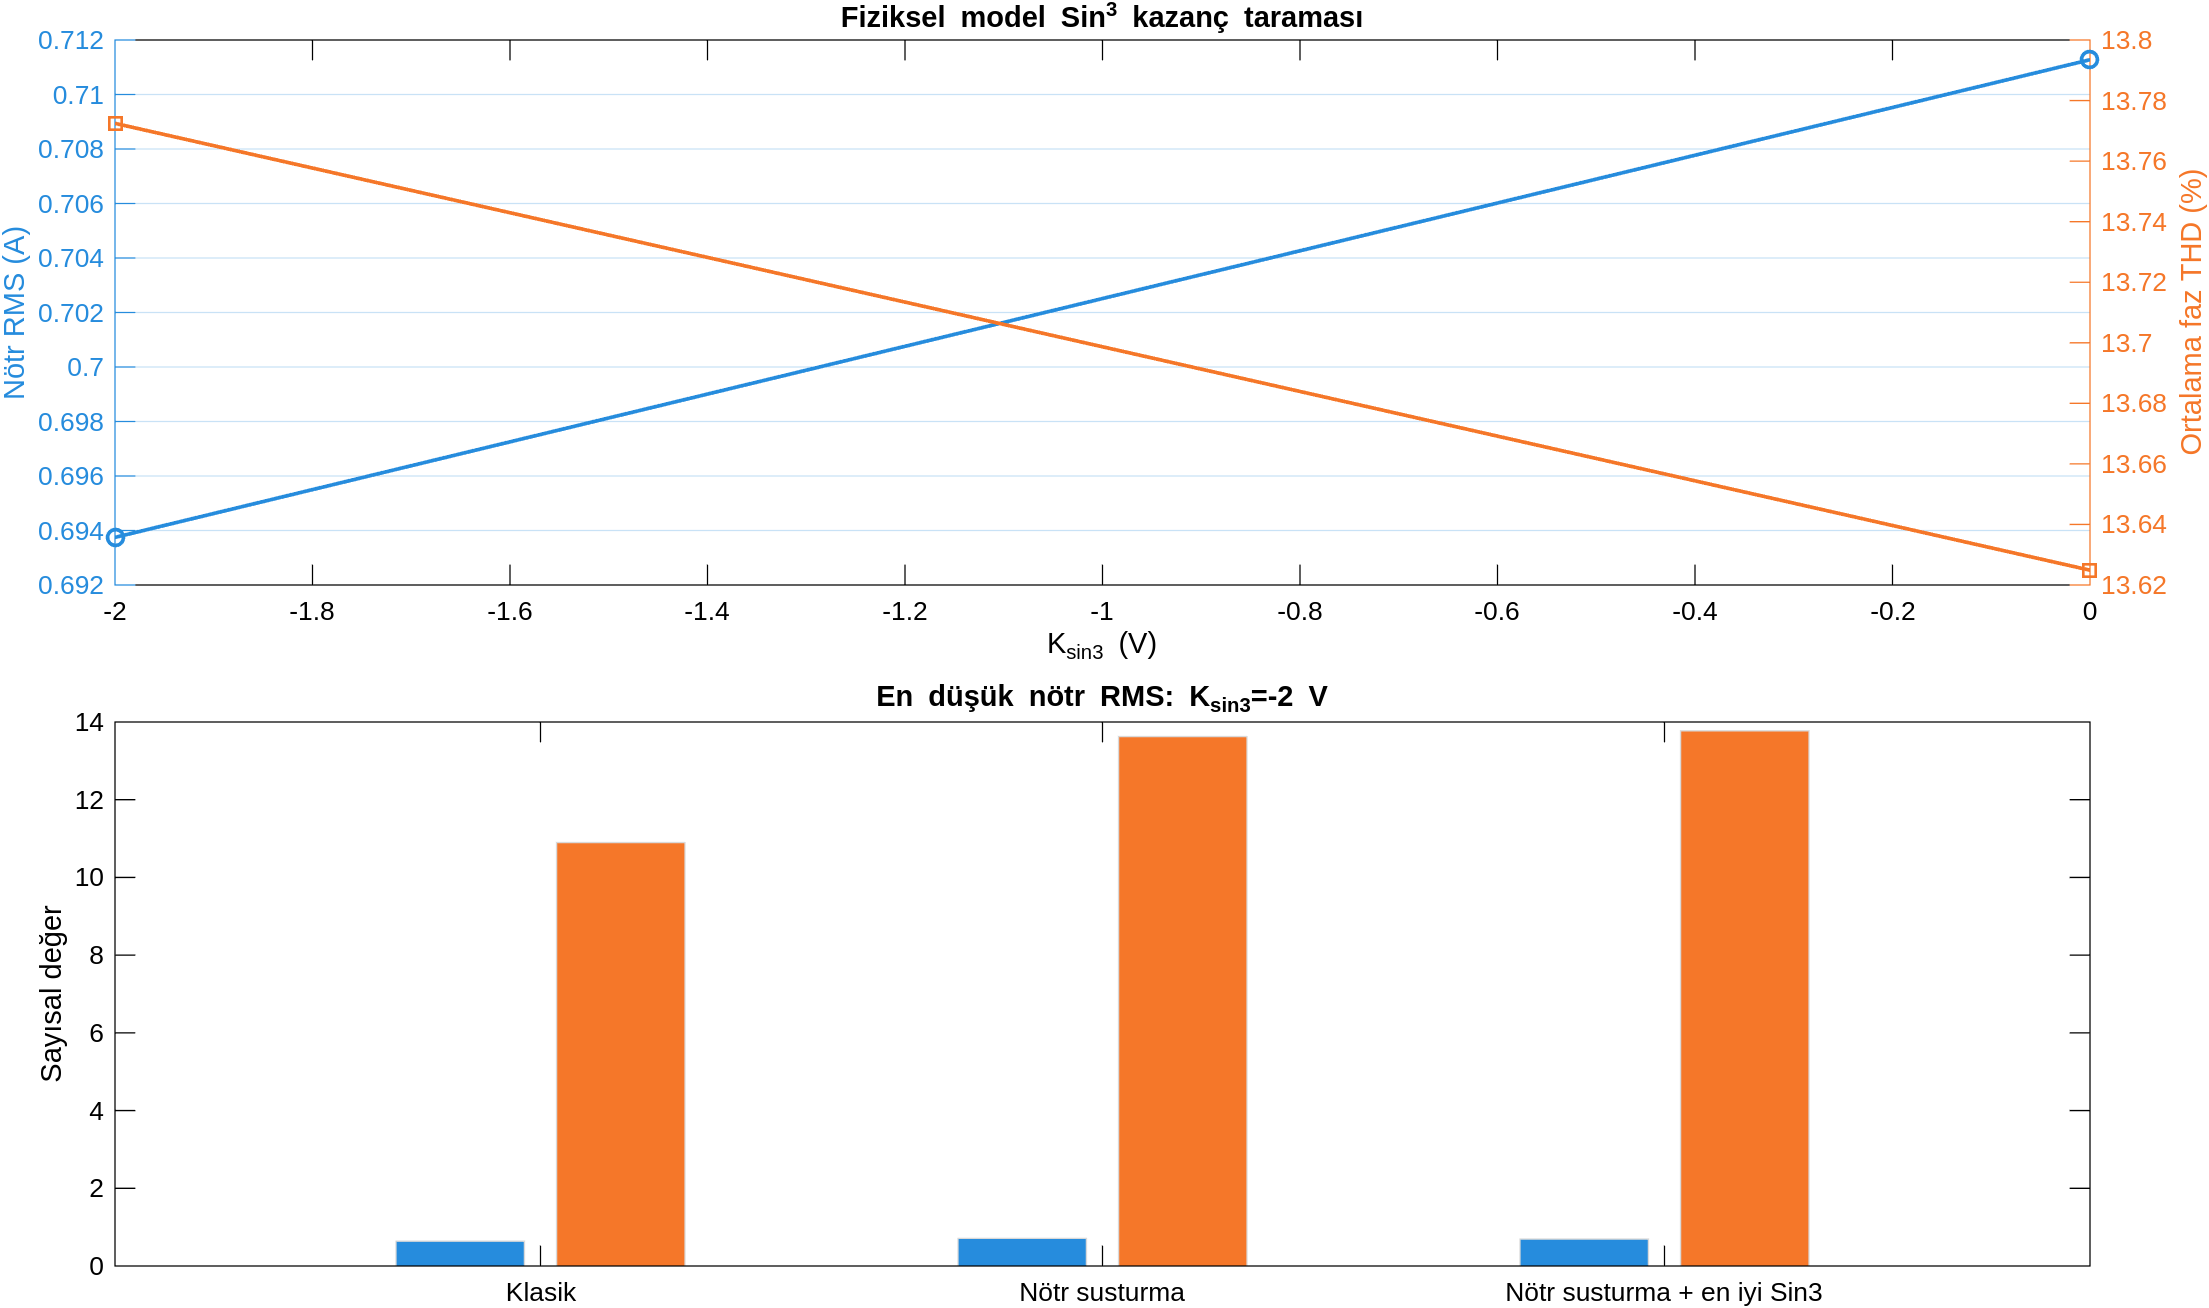
\includegraphics[width=0.96\textwidth]{sonuclar/fiziksel_senaryo123_20260822.png}
  \caption{Üç fazlı fiziksel yeniden koşuda nötr RMS ve ortalama faz THD karşılaştırması. Sonuçlar geçici fiziksel model parametreleriyle sınırlıdır.}
  \label{fig:yeniden-uretim-fiziksel-s123}
\end{figure}

Senaryo~4 için ayrıca, verilen $L_1=\SI{600}{\micro\henry}$, $R_1=\SI{0.02}{\ohm}$, $V_{\mathrm{dc}}=\SI{431}{\volt}$ ve \SI{120}{\volt} RMS şebeke değerleriyle ortalama-değerli bir akım-döngüsü fizibilite deneyi yapılmıştır. İleri besleme $K_1\sin(\theta+\phi)+K_3\sin^3(\theta)$ biçiminde, geri besleme ise $L_1$ akımıyla çalışan PI çıkışı olarak aynı gerilim komutunda toplanmıştır. Hedef ``30~A'' ifadesi tepe mi RMS mi belirtmediğinden iki yorum da sınanmıştır. PI kazançları $K_p=\SI{3}{\volt\per\ampere}$ ve $K_i=\SI{100}{\volt\per\ampere\second}$, denetim periyodu \SI{100}{\micro\second} ve $K_3=-\SI{2}{\volt}$ seçilmiştir.

\begin{table}[htbp]
  \centering
  \caption{Senaryo~4 ortalama-değerli PI fizibilite deneyi; yarı iletken anahtarlama kaybı ve verim kapsam dışıdır.}
  \label{tab:senaryo4-pi-30a}
  \small
  \begin{tabularx}{\textwidth}{p{0.17\textwidth} X r r r r}
    \toprule
    30 A yorumu & Denetim & Ölçülen RMS (A) & RMSE (A) & THD (\%) & $|m|_{\max}$ \\
    \midrule
    Tepe (21,213 A RMS) & İleri besleme & 11,742 & 11,187 & 5,326 & 0,781 \\
    Tepe (21,213 A RMS) & İleri besleme+PI & 20,922 & 0,665 & 0,559 & 0,791 \\
    RMS & İleri besleme & 20,138 & 11,135 & 3,103 & 0,783 \\
    RMS & İleri besleme+PI & 29,715 & 0,662 & 0,393 & 0,793 \\
    \bottomrule
  \end{tabularx}
\end{table}

Her iki PI koşusunda da modülasyon doyumu oluşmamış ve referans izleme belirgin biçimde iyileşmiştir. Şekil~\ref{fig:senaryo4-pi-30a}, son iki periyottaki akımları ve modülasyon payını göstermektedir. Sonuç, yaklaşık 30~A akımın ileri besleme+PI yapısıyla ortalama modelde izlenebildiğini kanıtlar; anahtarlamalı LCL model, cihaz kayıpları, termal portlar ve gerçek PI kodu eklenmeden verim veya donanım kararlılığı iddiası kurmaz.

\begin{figure}[htbp]
  \centering
  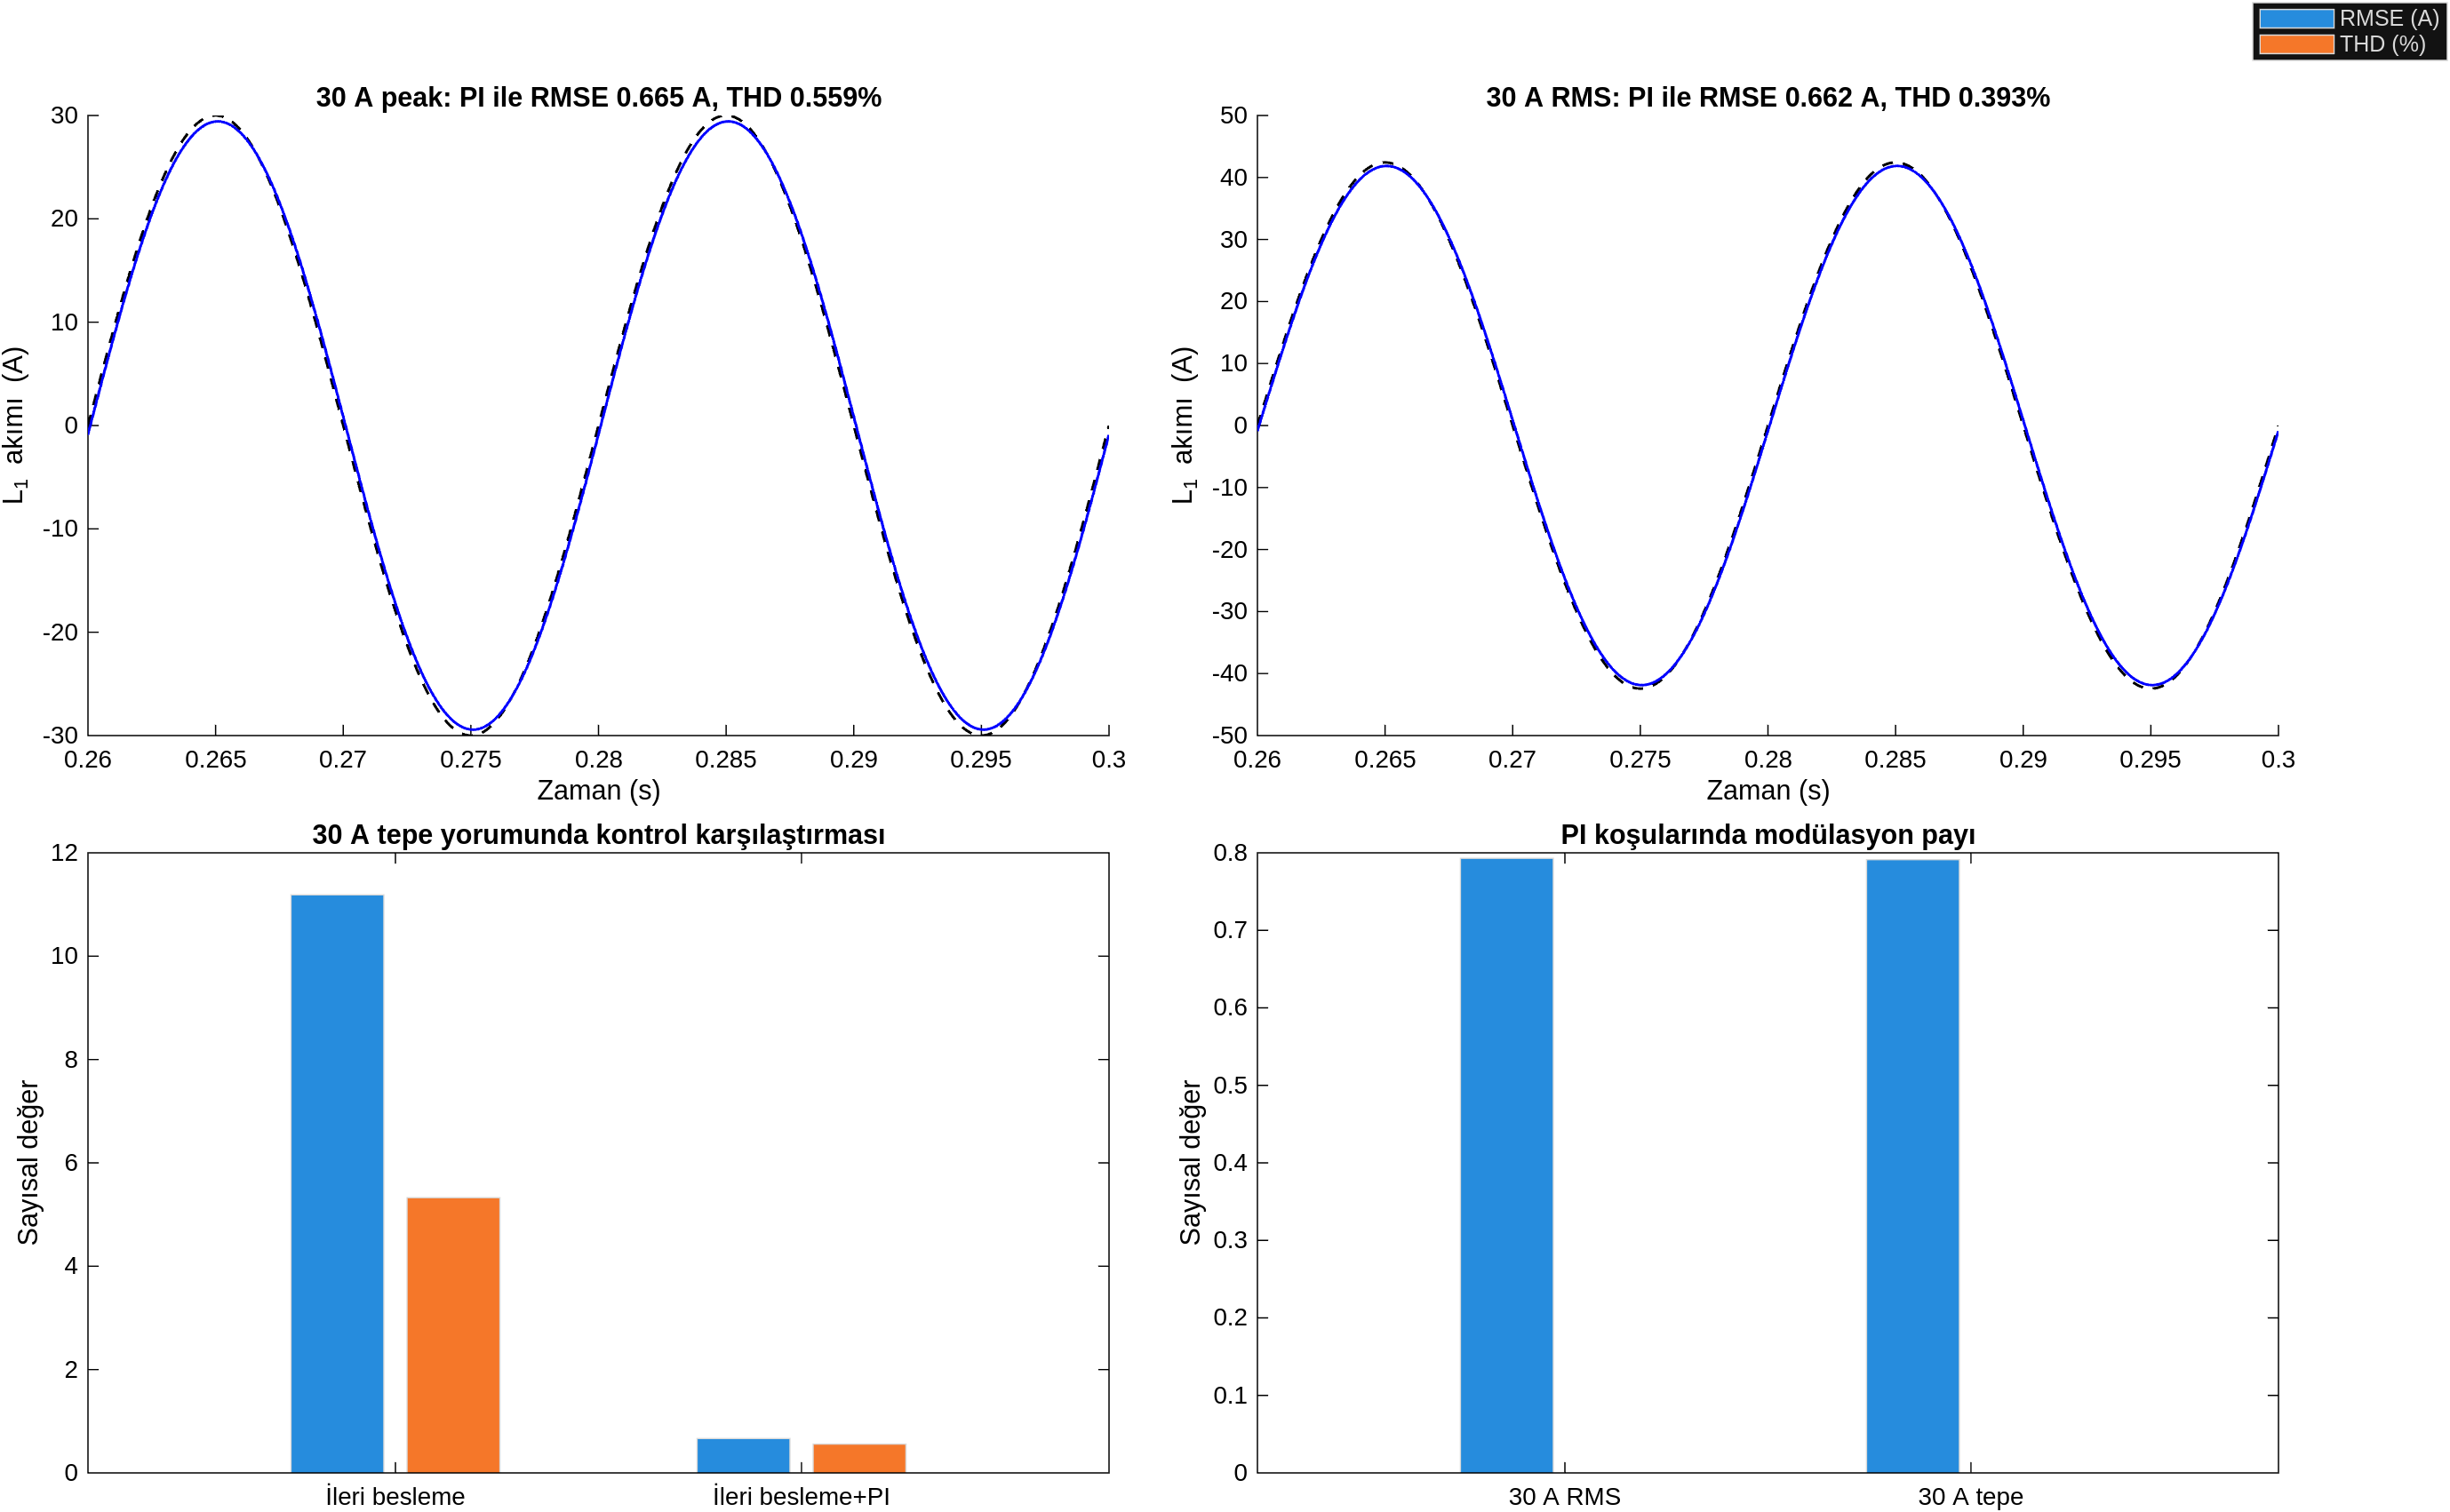
\includegraphics[width=0.98\textwidth]{sonuclar/senaryo4_pi_30a_20260822.png}
  \caption{Senaryo~4 için 30~A tepe ve 30~A RMS yorumlarında ileri besleme+PI akım izleme fizibilitesi ve modülasyon payı.}
  \label{fig:senaryo4-pi-30a}
\end{figure}

Nihai kazanç seçimi düşük güçte tek bir THD minimumuna göre yapılmayacaktır. Aday kazançlar önce düşük güçte ters akım--THD ödünleşimiyle taranacak, ardından orta ve nominal güçte kompanzasyonun gereksiz temel bileşen değişimi veya doyum üretmediği doğrulanacaktır. Aynı denetleyici katsayılarının bütün güç aralığında korunması hedeflenecek; kazanç çizelgelemesi gerekirse etkinleştirme eşiği, histerezis ve geçiş sürekliliği açıkça raporlanacaktır.

\section{Bölüm Sonucu}

Sin\textsuperscript{3} özdeşliği temel ve üçüncü harmonik bileşenini tek bir anlık terimde birleştirmekte, ancak doğrudan $\sin(3\theta)$ enjeksiyonuyla aynı katsayı anlamını taşımamaktadır. DCM/CCM parçalı modeli, nötr susturma sonrasında sinüzoidal görev oranının neden sinüzoidal akım üretmediğini göstermiş; doğru özdeşlikle yapılan katsayı taraması saf sinüs görev oranındaki \%39,96'lık üçüncü harmonik oranını, doğrulanmış parametre setiyle uyumlu $(D_1,D_3)=(0{,}34,\ 0{,}40)$ noktasında \%0,15'e indiren düzeltilmiş bir aday üretmiştir. Aynı tarama, önceki aday katsayıların bu parametre setine taşınamadığını sayısal olarak göstermiştir; katsayı seçimi çalışma noktasına bağlıdır.

Kapalı çevrim yapı Sin\textsuperscript{3} terimini bağımsız kontrolcü olarak değil, akım döngüsünün modülasyon toplamına eklenen ileri besleme girişi olarak konumlandırmıştır. Geçici MATLAB modeli $L$, $S$ ve $T$ analiz zincirini ve şebeke endüktansı taramasını çalıştırmaktadır; sayısal kararlılık marjları gerçek parametre doğrulaması beklemektedir. Bağımsız fiziksel koşu tarihsel THD iyileşmesini yeniden üretmemiş ve gerçek enjeksiyon/kazanç eşleşmesinin zorunluluğunu göstermiştir. Senaryo~4 ortalama modeli, yaklaşık 30~A akımın PI ile doyumsuz izlenebildiğini göstermiştir; orta ve nominal güçte anahtarlamalı verim, termal durum, THD ve geçici rejim karşılaştırması gerçek model ve ölçüm verileriyle tamamlanmalıdır.

\chapter{DENEYSEL DOĞRULAMA}
\label{chap:deney}

Bölüm~\ref{chap:anahtarlama} ve Bölüm~\ref{chap:sin3} içinde benzetim düzeyinde incelenen klasik anahtarlama, nötr anahtar susturma ve susturma+Sin\textsuperscript{3} yöntemleri, geliştirilen üç fazlı T-tipi prototipin tek faz kolunda, düşük güç koşulunda karşılaştırılmıştır. Bölümde deney düzeneği, güç donanımı, denetim ve ölçüm zinciri testleri yeniden üretecek ayrıntıda tanıtılmakta; mevcut deney kayıtları kanıt sınırlarıyla birlikte değerlendirilmekte ve benzetim modelinin deney özetine kalibrasyonu (Kesim~\ref{sec:kalibrasyon}) verilmektedir. Tez kapsamında yeni deney yapılmamıştır; kayıtlar mevcut arşivden alınmış, metin, tablo ve ekran değerleri kaynak içi tutarlılık bakımından denetlenmiştir.

\textbf{Deneysel kanıtın kapsamı.} Eldeki deneysel kanıt üç yönteme ait PC yazılımı ekranları, osiloskop ekranları ve her yöntem için tek satırlık bir deney özet tablosudur (Tablo~\ref{tab:gelen-excel-senaryolar}). Enerjilendirme sırası, başlangıç koşulları, kararlı duruma geçiş ölçütü ve ölçüm süresini içeren deney protokolü; ham PC/Modbus ve osiloskop kayıtları; tekrar sayısı ve analizör kalibrasyon belgeleri belgelenmemiştir. Deney sonuçları, ekran ve özet tablosu düzeyinde destekleyici kanıt olarak kullanılmaktadır. Ölçüm belirsizliği yalnız üretici toleransları ve okuma çözünürlüğünden kestirilebilmekte, istatistiksel yayılım hesaplanamamaktadır. Benzetim modeli deney özetinin etkin ve reaktif gücüne kalibre edilmiş, diğer büyüklükler bağımsız karşılaştırma olarak raporlanmıştır (Kesim~\ref{sec:kalibrasyon}). Protokol ve ham kayıt eksikliği Bölüm~\ref{chap:sonuc} içinde sınırlılık olarak yer almaktadır.

\section{Deney Düzeneği ve Güç Donanımı}

Deney düzeneği, yaklaşık 20--25~kW güç dönüştürme kapasitesi hedeflenerek düşey bir pano üzerine bakır baralarla modüler biçimde kurulmuştur. Akım sensörü boyutlandırma hesabında prototip gücü \SI{20}{\kilo\volt\ampere} olarak verilmiştir; güç birimi ve anma değeri arasındaki fark, prototip etiketi veya tasarım dosyası bulunmadan tek bir anma değerinde birleştirilmemiştir. Raporlanan deneylerin yaklaşık \SI{2.3}{\ampere} faz akımında gerçekleştirilmesi, mevcut sonuçların anma gücü değil düşük güç doğrulaması olduğunu göstermektedir.

Şekil~\ref{fig:deney-duzenegi-genel}; varyak modülü, evirici panosu, bilgisayar ve osiloskopları aynı görünümde vermektedir. Varyak modülünde enerji bağlantıları, şalt ve koruma ekipmanları, akım transformatörleri ve AA enerji analizörü bulunmakta; üç faz bağımsız varyaklarla ayarlanabilmektedir. Aşırı akım, kaçak akım, topraklama ve acil durdurma önlemleri mevcuttur; eşik ve açma süreleri kaynak kayıtlarda yer almamaktadır.

\begin{figure}[htbp]
  \centering
  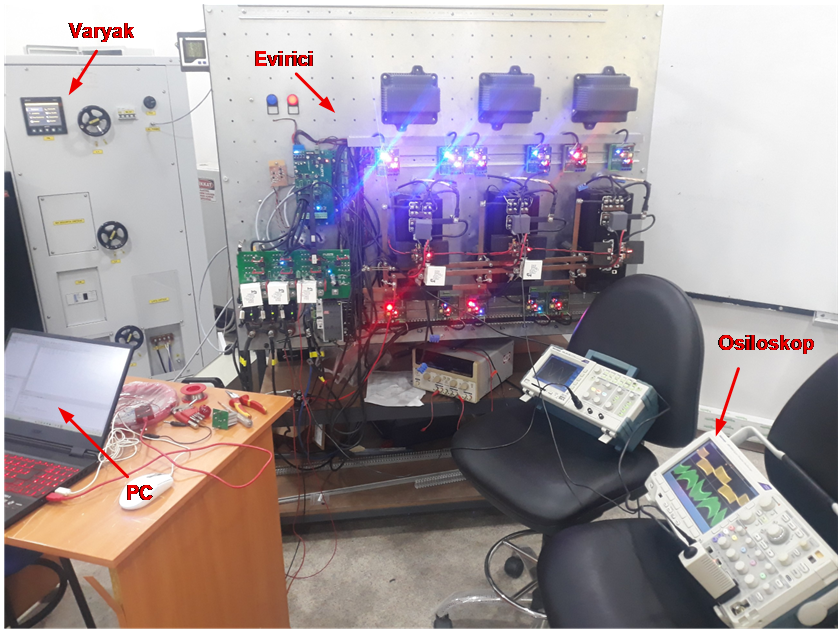
\includegraphics[width=0.95\textwidth]{deneysel/onceki_tez_sekil_5_1_deney_duzenegi.png}
  \caption{Deney ve ölçme düzeneklerinin genel görünümü.}
  \label{fig:deney-duzenegi-genel}
\end{figure}

Şekil~\ref{fig:deney-evirici-genel}, evirici donanımının önden genel görünümünü sunmaktadır. Üç faza ait güç modülleri, kontrol ve ölçüm kartları, DA bara bağlantıları ve yardımcı beslemeler aynı pano üzerindedir; genel görünüm, numaralı ayrıntıların verildiği Şekil~\ref{fig:deney-donanim-kartlar} için yerleşim bağlamı sağlamaktadır.

\begin{figure}[htbp]
  \centering
  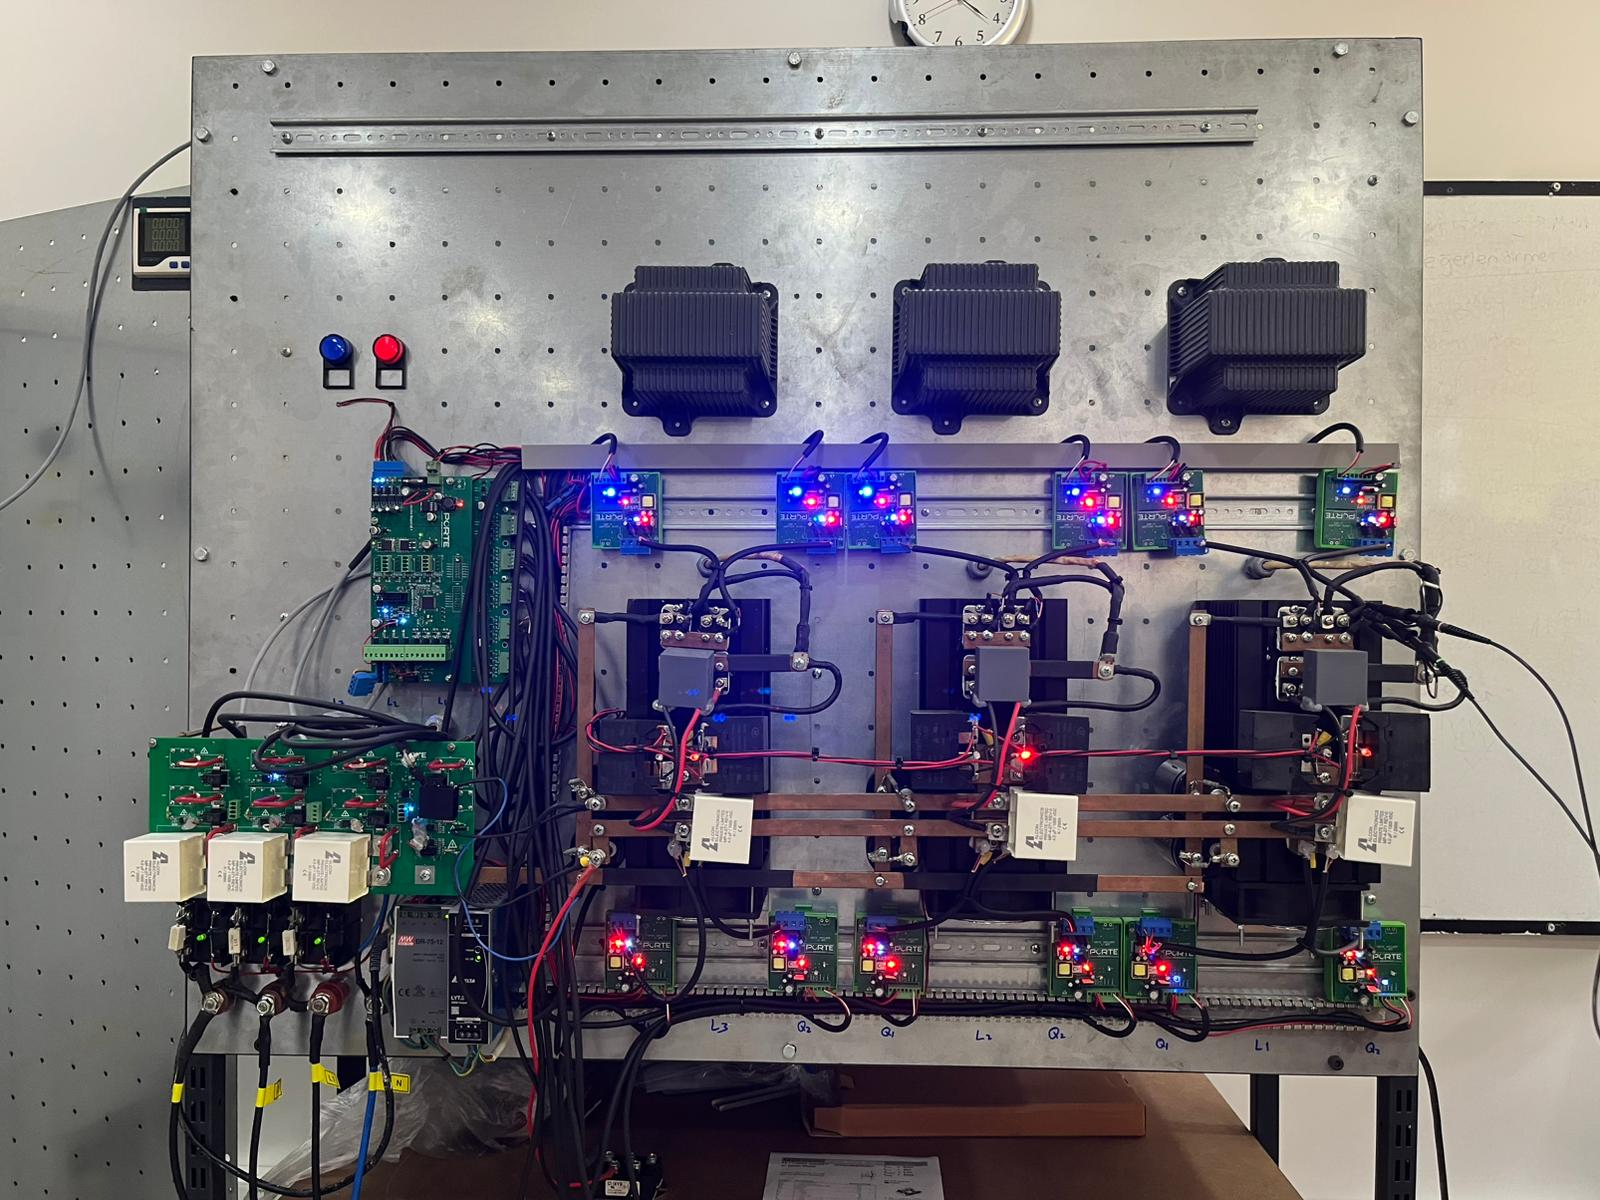
\includegraphics[width=0.88\textwidth]{deneysel/onceki_tez_sekil_5_2_evirici_donanimi.jpeg}
  \caption{Evirici donanımının genel görünümü.}
  \label{fig:deney-evirici-genel}
\end{figure}

Şekil~\ref{fig:deney-donanim-kartlar} üzerindeki 1--14 numaraları doğrudan Tablo~\ref{tab:deney-alt-birimler} içindeki açıklamalara karşılık gelmektedir.

\begin{figure}[htbp]
  \centering
  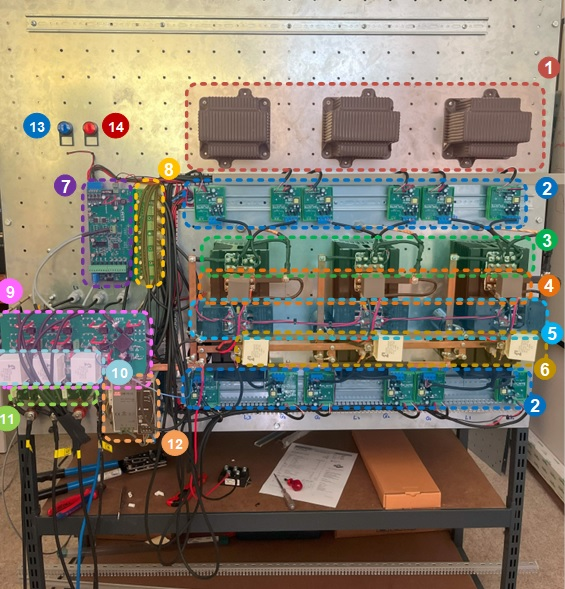
\includegraphics[width=0.72\textwidth]{deneysel/onceki_tez_sekil_5_3_donanim_alt_birimleri.jpeg}
  \caption{Evirici donanımı ve alt birimlerinin numaralı tanıtımı.}
  \label{fig:deney-donanim-kartlar}
\end{figure}

\clearpage
\begin{table}[htbp]
  \centering
  \caption{Evirici donanımının alt birimleri.}
  \label{tab:deney-alt-birimler}
  \small
  \begin{tabularx}{0.94\textwidth}{X X}
    \toprule
    1. LCL filtrelerin $L_1$ bobinleri & 2. IGBT kapı sürme kartları \\
    3. Nötr IGBT'leri & 4. Yükseltici (boost) diyotları \\
    5. Fonksiyon değiştirme röleleri & 6. Snubber kapasitörleri \\
    7. Kontrol kartı & 8. Tampon (buffer) kartı \\
    9. Ölçme kartı & 10. LCL filtre kapasitörleri \\
    11. Ani akım (inrush) röleleri & 12. Kumanda beslemeleri \\
    13. Şarj fonksiyonu lambası & 14. Deşarj fonksiyonu lambası \\
    \bottomrule
  \end{tabularx}
\end{table}

Şekil~\ref{fig:deney-faz-donanim-1} ve Şekil~\ref{fig:deney-faz-donanim-2}, aynı faz kolunun iki farklı açıdan çekilmiş ayrıntılarını göstermektedir; her iki görseldeki 1--8 numaraları Tablo~\ref{tab:deney-faz-komponentler} ile birlikte okunmalıdır. İki görüntünün ayrı tutulması; boost diyotları, fonksiyon değiştirme röleleri, DA bara ve snubber kapasitörleri, soğutma düzeni, sürücü kartı ve $L_1$ bobininin fiziksel konumunu kaybetmeden izlemeyi sağlamaktadır.

\begin{figure}[htbp]
  \centering
  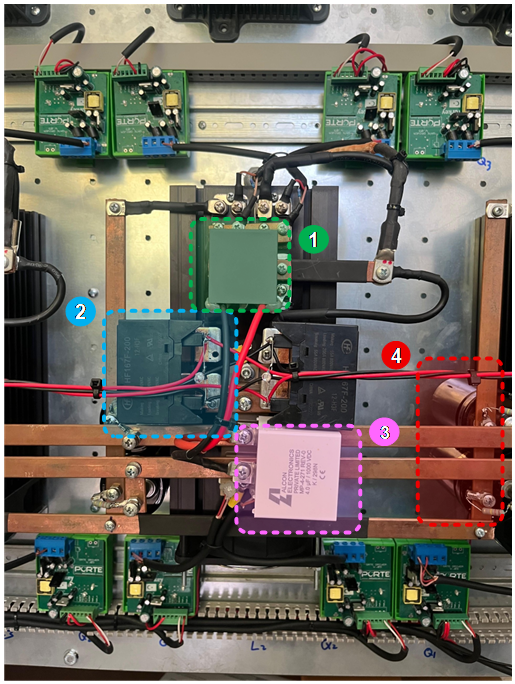
\includegraphics[height=0.68\textheight]{deneysel/onceki_tez_sekil_5_4_faz_donanimlari_1.png}
  \caption{Eviricinin bir fazına ait donanımlar, birinci görünüm.}
  \label{fig:deney-faz-donanim-1}
\end{figure}

\begin{figure}[htbp]
  \centering
  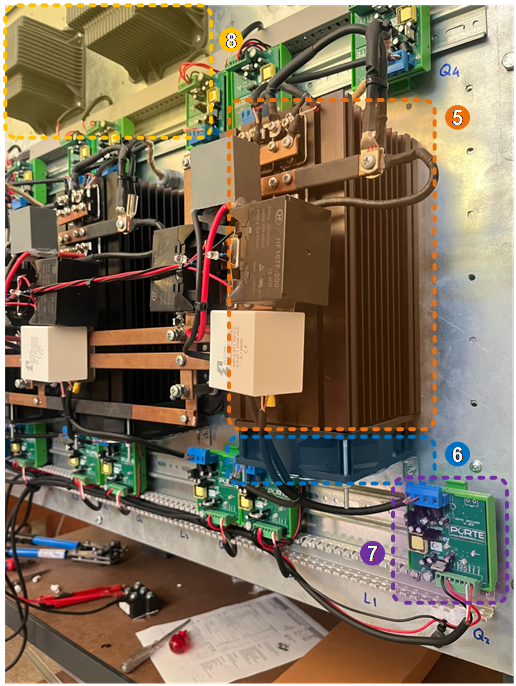
\includegraphics[height=0.68\textheight]{deneysel/onceki_tez_sekil_5_5_faz_donanimlari_2.png}
  \caption{Eviricinin bir fazına ait donanımlar, ikinci görünüm.}
  \label{fig:deney-faz-donanim-2}
\end{figure}

\clearpage
\begin{table}[htbp]
  \centering
  \caption{Şekil~\ref{fig:deney-faz-donanim-1} ve Şekil~\ref{fig:deney-faz-donanim-2}'deki faz donanımı bileşenleri.}
  \label{tab:deney-faz-komponentler}
  \small
  \begin{tabularx}{0.94\textwidth}{X X}
    \toprule
    1. Boost diyotları ve kondansatörü & 2. Fonksiyon değiştirme röleleri \\
    3. Snubber kondansatörleri & 4. DA bara elektrolitik kondansatörleri \\
    5. IGBT soğutucu & 6. Yüksek devirli soğutma fanı \\
    7. IGBT kapı sürme kartı & 8. LCL filtre $L_1$ bobini \\
    \bottomrule
  \end{tabularx}
\end{table}

Şekil~\ref{fig:deney-giris-devresi}, evirici giriş devresini ve 1--6 ile işaretlenmiş yardımcı donanımları göstermektedir; numaraların karşılığı Tablo~\ref{tab:deney-giris-komponentler} içindedir. Giriş bölümünün ayrı verilmesi; inrush röleleri, sigorta, yardımcı kaynaklar, EMI filtresi, kontrol kartı ve tampon kartının güç katıyla bağlantısını görünür kılmaktadır.

\begin{figure}[htbp]
  \centering
  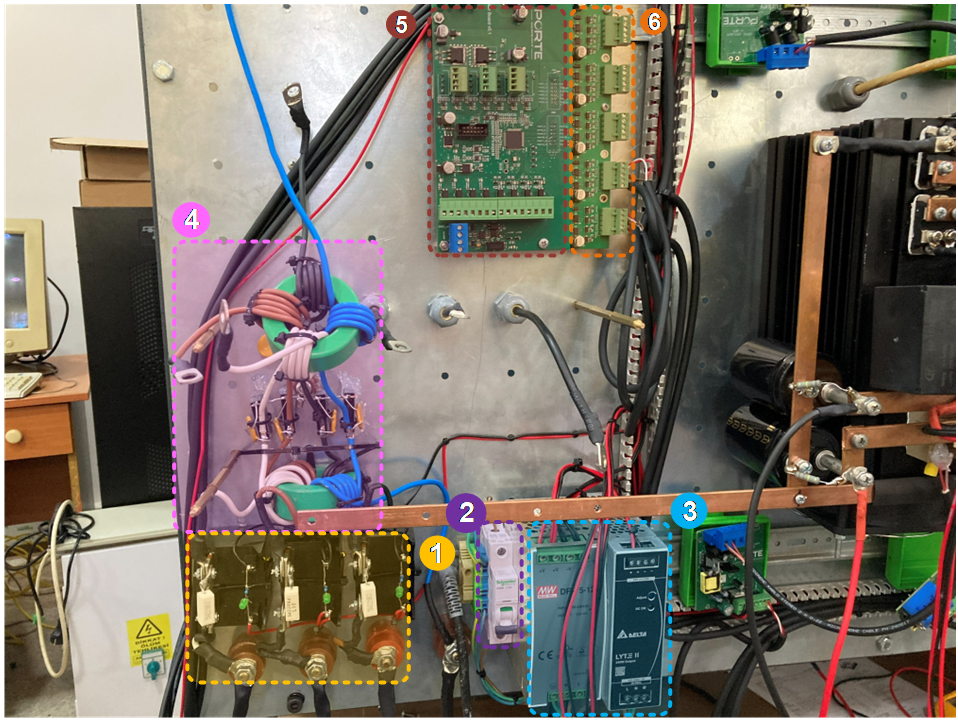
\includegraphics[width=0.94\textwidth]{deneysel/onceki_tez_sekil_5_6_giris_devresi.png}
  \caption{Evirici giriş devresinin ayrıntı görünümü.}
  \label{fig:deney-giris-devresi}
\end{figure}

\clearpage
\begin{table}[htbp]
  \centering
  \caption{Evirici giriş kısmına ait bileşenler.}
  \label{tab:deney-giris-komponentler}
  \small
  \begin{tabularx}{0.94\textwidth}{X X}
    \toprule
    1. Ani akım (inrush) röleleri & 2. Evirici açma kapama sigortası \\
    3. 12 V--24 V güç kaynakları & 4. EMI filtre \\
    5. Kontrol kartı & 6. Tampon (buffer) kartı \\
    \bottomrule
  \end{tabularx}
\end{table}

\section{Kontrol Kartı, Tampon Kartı ve Kapı Sürücüsü}

Şekil~\ref{fig:deney-kontrol-buffer}, kontrol ve tampon kartlarını numaralı işlevleriyle göstermektedir. Kontrol kartında RS485 haberleşme birimi, optoizole giriş/çıkışlar, DA bara ve akım ölçüm dönüştürme devreleri, PIC32MK ailesi mikrodenetleyici, lineer regülatörler ve röle/fan çıkış katları bulunmaktadır. Tampon kartı, mikrodenetleyicinin \SI{3.3}{\volt} tek uçlu (single-ended) PWM işaretlerini diferansiyel sinyal çiftlerine dönüştürmek ve uzun ekranlı kablolarda ortak-mod gürültü etkisini azaltmak amacıyla kullanılmıştır. Fotoğraftaki numaralar sırasıyla şu işlevleri gösterir: (1) RS485 haberleşme; (2)--(3) optoizole giriş ve çıkışlar; (4) diferansiyel DA bara gerilimini tek uçlu biçime dönüştüren ölçüm katı; (5) ölçüm, haberleşme ve kontrol algoritmalarını yürüten PIC32MK mikrodenetleyici; (6) akım ölçüm dönüştürme katı; (7) \SI{5}{\volt} lineer regülatörler; (8) röle ve fanlar için MOSFET güç çıkışları; (9) \SI{9}{\volt} anahtarlamalı regülatör; (10) PWM tampon kartının \SI{9}{\volt} beslemesi; (11) tek uçlu PWM işaretlerini diferansiyel çiftlere dönüştüren kat.

\begin{figure}[htbp]
  \centering
  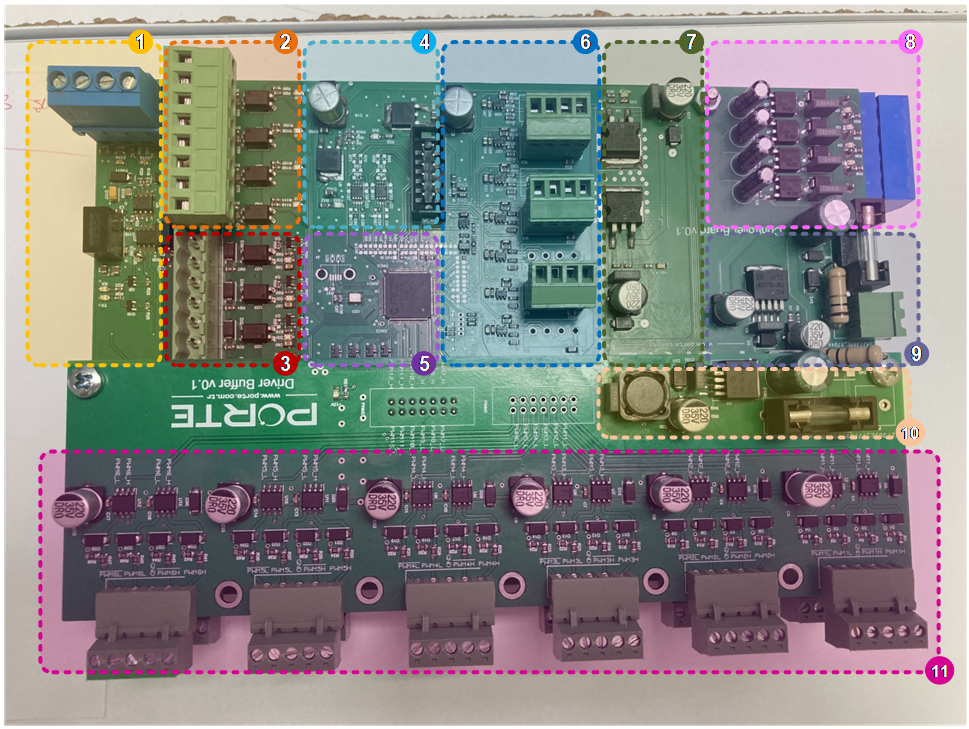
\includegraphics[width=0.90\textwidth]{deneysel/onceki_tez_sekil_5_7_kontrol_buffer.png}
  \caption{Kontrol kartı ve tampon kartının numaralı görünümü.}
  \label{fig:deney-kontrol-buffer}
\end{figure}

PWM1--PWM6 kanallarının yüksek ve alçak işaretleri tampon kartında diferansiyel çiftlere dönüştürülmekte; yaklaşık \SI{12}{\volt} genlikte, tek yönlü iletim amacıyla H-köprü tabanlı bir sürme çözümü kullanılmaktadır. Gerçek PWM kaynak kodu, ölü zaman, minimum darbe süresi ve çıkış gecikmeleri mevcut olmadığından zincirin zamanlama performansı henüz doğrulanamamıştır.

Şekil~\ref{fig:deney-igbt-surucu}, ADuM4135 tabanlı IGBT kapı sürme kartını göstermektedir. Diferansiyel giriş, desatürasyon koruması, aktif Miller kenetleme ve düşük gerilim kilitleme özellikleri sürücü seçiminin gerekçeleridir: diferansiyel giriş uzun PWM hatlarındaki ortak-mod gürültüsüne bağışıklık sağlar; desatürasyon koruması aşırı akımda IGBT komutunu donanımsal olarak keser; aktif Miller kenetleme yüksek frekanslı anahtarlamada hatalı iletime geçme (false turn-on) riskini azaltır. Bütün sürücülerden gelen FAULT çıkışları kontrol kartında toplanmakta ve ortak RESET işareti sürücülere paralel dağıtılmaktadır; böylece donanım koruması ile denetim yazılımı arasında bir hata yönetim zinciri oluşmaktadır.

\begin{figure}[htbp]
  \centering
  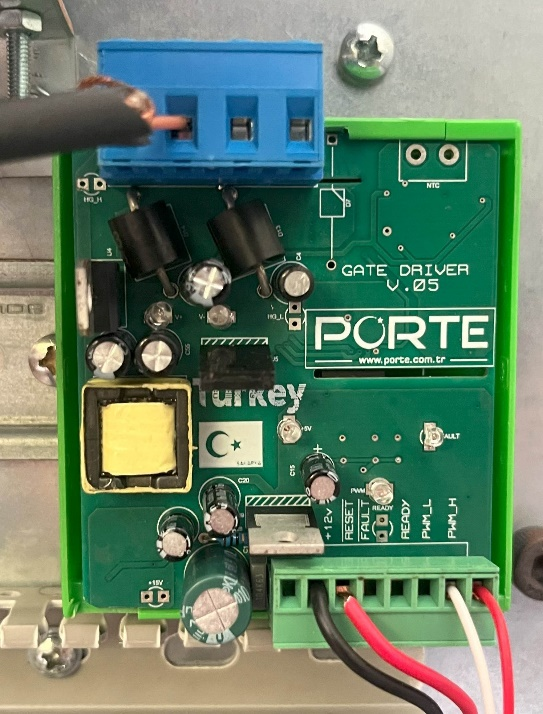
\includegraphics[height=0.64\textheight]{deneysel/onceki_tez_sekil_5_8_igbt_surucu.jpeg}
  \caption{IGBT kapı sürme devresi.}
  \label{fig:deney-igbt-surucu}
\end{figure}

\clearpage
\section{Gerilim ve Akım Ölçme Devreleri}

Faz--nötr gerilimleri ile pozitif ve negatif DA bara gerilimleri, AMC1200 tabanlı izole ölçüm devreleriyle alınmaktadır; ölçüm kartının ofset, ADC aralığı ve DA bara ölçüm aralığı Tablo~\ref{tab:sistem-parametreleri} içindedir. AMC1200'ün gerilim kazancı 8 olduğundan girişte izin verilen en yüksek genlik \SI{162.5}{\milli\volt} olarak hesaplanmış; faz ve DA bara ölçümleri için ayrı gerilim bölücüler kullanılmıştır. Faz ölçüm sınırı anlık yaklaşık \SI{387}{\volt}'tur.

Mikrodenetleyicideki yedi ADC kanalının üçü faz--nötr gerilimlerine, ikisi pozitif ve negatif DA bara gerilimlerine ayrılmıştır. Faz ölçümleri AMC1200 çıkışlarından ekranlı kabloyla diferansiyel olarak taşınmış ve RC örtüşme önleme (anti-aliasing) filtrelerinden geçirilmiştir. DA bara kanallarında diferansiyel işaretler enstrümantasyon yükselteciyle işlenip \SI{1.3}{\volt} ofset eklenerek tek uçlu biçime dönüştürülmektedir. 12 bit ADC gösterimi, diferansiyel sayısal aralığı yaklaşık $-2047$ ile $+2048$ arasında tanımlamaktadır.

Dört telli T-tipi yapıda nötr noktasının kayması iki DA bara kondansatörünün gerilimlerini eşitsizleştirebileceğinden pozitif ve negatif bara kanalları sürekli izlenmekte; eşik aşımında mikrodenetleyici FAULT üretip PWM çıkışlarını kesmektedir. AMC1200 giriş beslemesi RFM-0505S izole dönüştürücü ile sağlanmış; dönüştürücü çıkışındaki regülasyon zayıflığını azaltmak için TCR2EF250 düşük gerilim düşümlü regülatör kullanılmıştır. Ölçüm zinciri böylece yalnız ölçekleme değil, izolasyon ve nötr nokta koruması görevlerini de üstlenmektedir.

Akım ölçümünde HLSR 20-P/SP33 Hall etkili sensör kullanılmıştır. Sensör kazancı ve ölçülebilir simetrik tepe akımı Tablo~\ref{tab:sistem-parametreleri} içindedir; tepe sınırın RMS karşılığı yaklaşık \SI{39.9}{\ampere}'dir. Faz başına akım tasarım değeri ve yüzde 20 paylı üst sınırı aynı tabloda verilmiştir. Hesaplar nominal direnç değerlerine dayanır; gerçek direnç toleransları, ADC kalibrasyonu ve sensör sıcaklık sapmasıyla doğrulanmamıştır.

Ani faz ve kondansatör akımlarının sınırlandırılması amacıyla kullanılan pencere karşılaştırıcı devre Şekil~\ref{fig:deney-pencere-karsilastirici} üzerinde verilmiştir. Devrede üst eşik \SI{2.0}{\volt}, alt eşik \SI{0.6}{\volt} olarak, sensör referansına simetrik ayarlanmıştır. Eşiklerin referanstan uzaklığı, sensör kazancıyla Tablo~\ref{tab:sistem-parametreleri} içindeki aşırı akım eşiğine karşılık gelmektedir. Eşik dışına çıkıldığında FAULT işareti kontrol kartında harici kesme oluşturarak PWM çıkışlarını kesmektedir.

\begin{figure}[htbp]
  \centering
  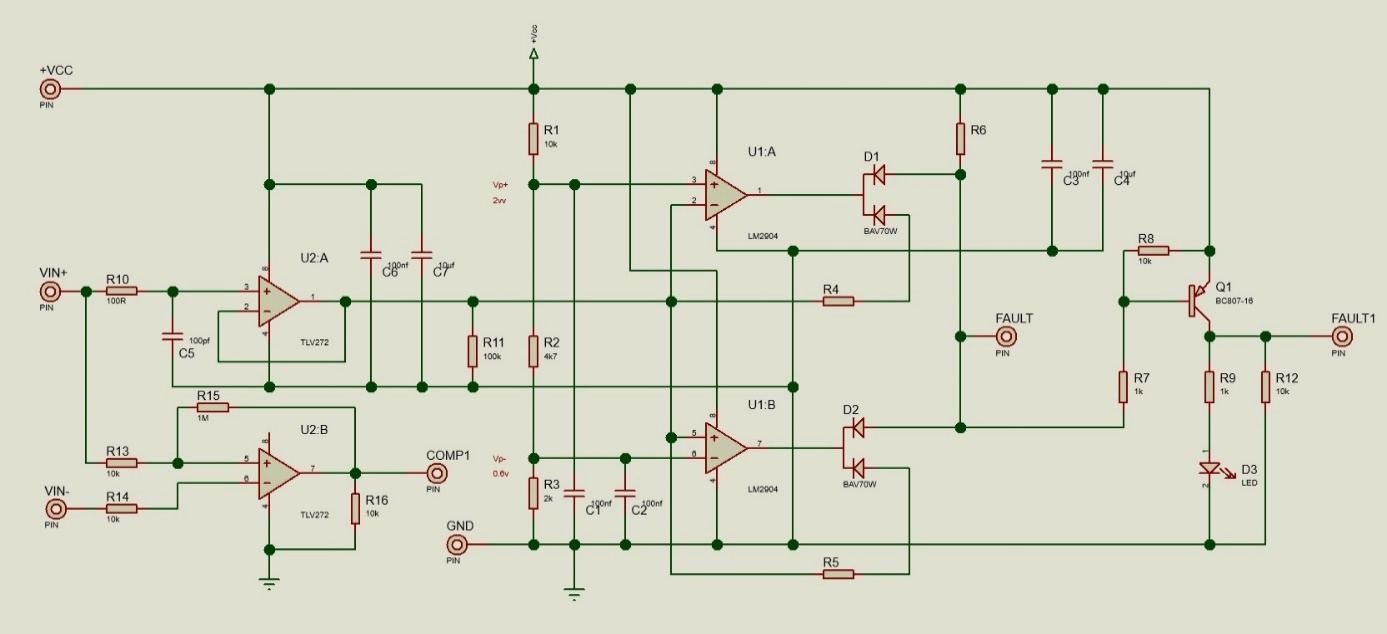
\includegraphics[width=0.96\textwidth]{deneysel/onceki_tez_sekil_5_9_pencere_karsilastirici.jpeg}
  \caption{Pencere karşılaştırıcı devresi.}
  \label{fig:deney-pencere-karsilastirici}
\end{figure}

Şekil~\ref{fig:deney-pencere-dalga}, harici bir deneme kartının DAC çıkışıyla uygulanan giriş işareti ve pencere karşılaştırıcının FAULT çıkışını göstermektedir. İmleç seviyeleri \SI{2.0}{\volt} ve \SI{0.6}{\volt} olarak ayarlanmış; giriş sınırların dışına çıktığında ikinci kanal işaretinin lojik sıfıra indiği gözlenmiştir. Kayıt, koruma mantığının işlevsel örneğidir; gecikme süresi ve gerçek kısa devre kesme enerjisi aynı görüntüden çıkarılamaz.

\begin{figure}[htbp]
  \centering
  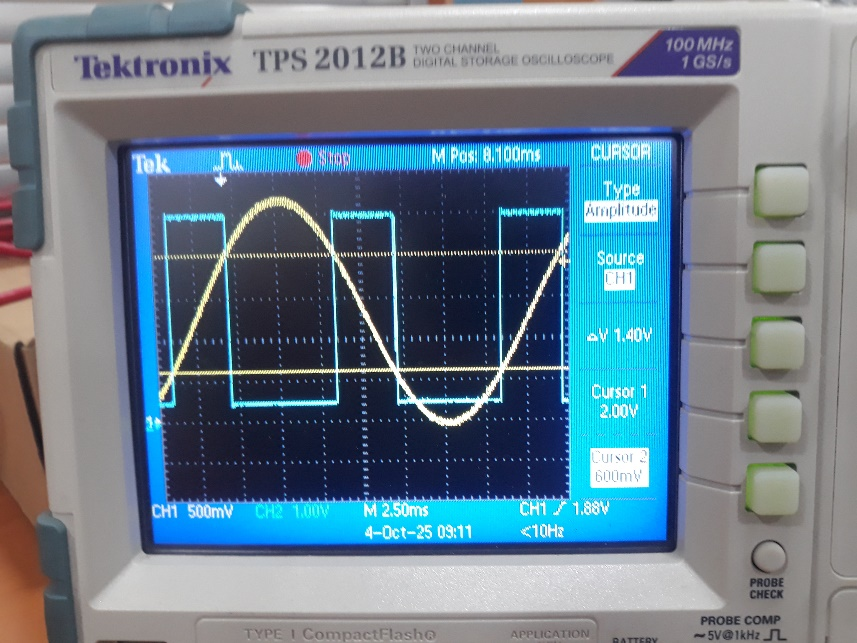
\includegraphics[width=0.88\textwidth]{deneysel/onceki_tez_sekil_5_10_pencere_dalga.jpeg}
  \caption{Pencere karşılaştırıcı giriş ve çıkış gerilim dalga şekilleri.}
  \label{fig:deney-pencere-dalga}
\end{figure}

Şekil~\ref{fig:deney-olcum-karti}; HLSR akım sensörleri, AMC1200 izole ölçüm kanalları ve akım probu bağlantı iletkenlerini içeren ölçüm kartını göstermektedir. Kart üzerindeki \SI{4}{\milli\metre\squared} kesitli ters-U biçimli iletkenler; faz başına $L_1$ akımı, kondansatör akımı ve faz akımının ayrı ayrı osiloskop probuyla ölçülmesini sağlamaktadır. TLV431 referansları ve MC33269 regülatörleri ölçüm beslemesi ile \SI{1.3}{\volt} ofset üretiminde kullanılmıştır.

\begin{figure}[htbp]
  \centering
  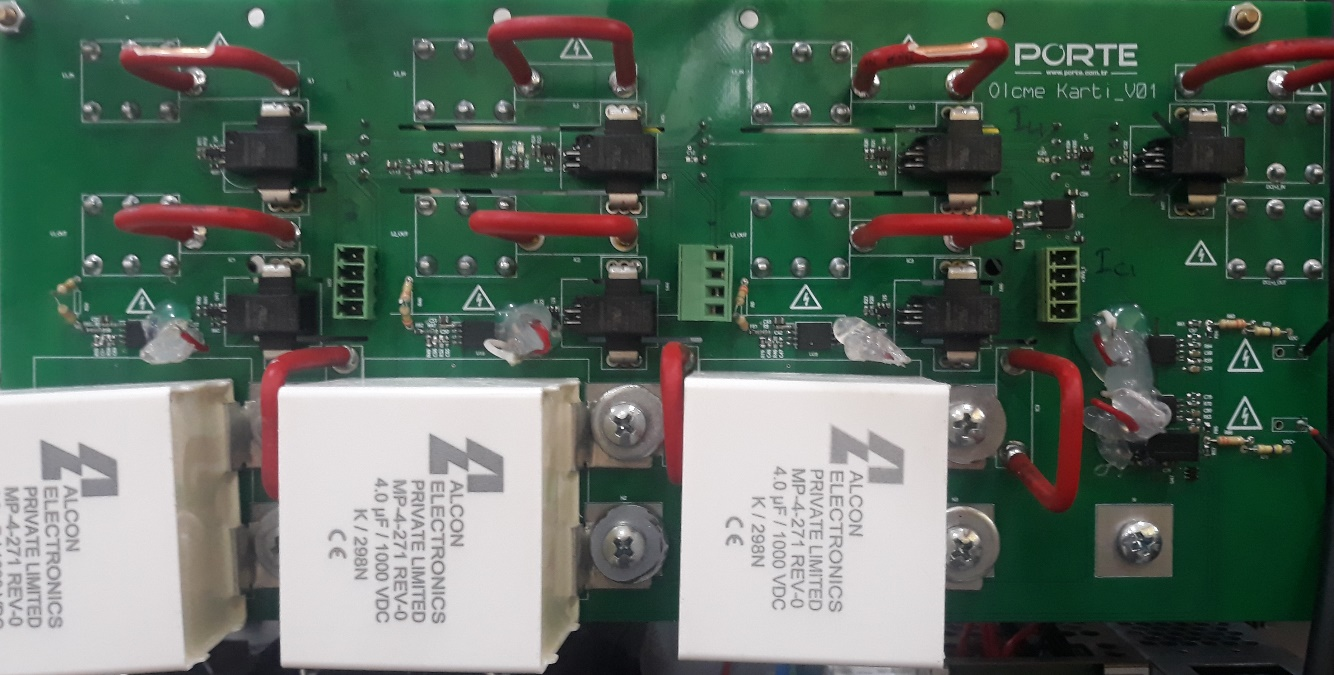
\includegraphics[width=0.96\textwidth]{deneysel/onceki_tez_sekil_5_11_olcum_karti.jpeg}
  \caption{Ölçüm kartı.}
  \label{fig:deney-olcum-karti}
\end{figure}

\section{DA ve AA Güç Analizörleri}

DA bara gerilimi, akımı ve gücü Accuenergy AcuDC240 analizörüyle ölçülmüştür; üretici akım ve gerilim için yüzde 0,2, güç ve enerji için yüzde 0,5 hata toleransı bildirmektedir. Şekil~\ref{fig:deney-acudc240}(a) cihazın pano üzerindeki konumunu, Şekil~\ref{fig:deney-acudc240}(b) üretici dokümanındaki şönt bağlantısını göstermektedir.

\begin{figure}[htbp]
  \centering
  \begin{subfigure}[t]{0.46\textwidth}
    \centering
    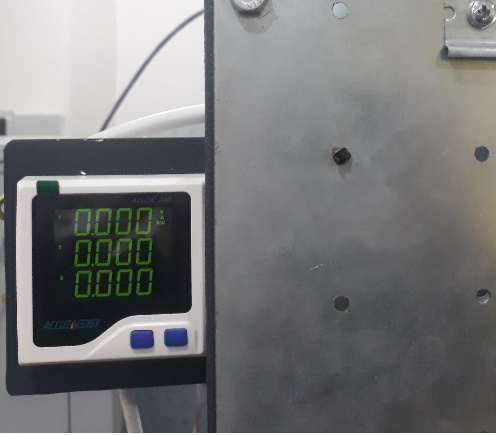
\includegraphics[width=\linewidth]{deneysel/onceki_tez_sekil_5_12a_acudc240.jpeg}
    \caption{Evirici donanımı üzerindeki AcuDC240.}
  \end{subfigure}\hfill
  \begin{subfigure}[t]{0.50\textwidth}
    \centering
    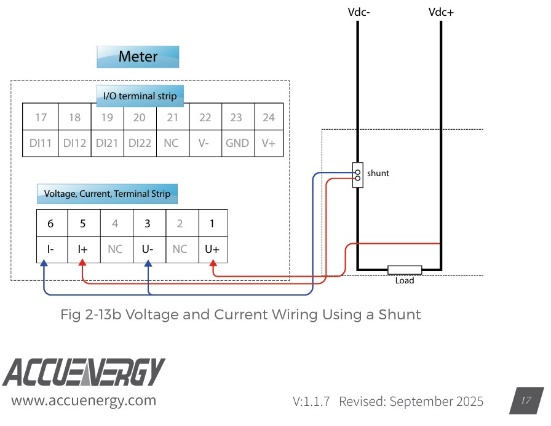
\includegraphics[width=\linewidth]{deneysel/onceki_tez_sekil_5_12b_acudc240_baglanti.jpeg}
    \caption{DA analizörü ve şönt bağlantı şekli.}
  \end{subfigure}
  \caption{AcuDC240 DA bara analizörü ve bağlantısı.}
  \label{fig:deney-acudc240}
\end{figure}

Prototipte şönt direnci DA baranın negatif terminaline bağlanarak alçak-taraf akım ölçümü yapılmıştır. Şekil~\ref{fig:deney-sont-baglanti}, \SI{20}{\ampere}/\SI{60}{\milli\volt} şönt direncin fiziksel bağlantısını göstermektedir. Şöntün ölçüm uçları koaksiyel ve ekranlı kabloyla analizöre taşınmış; DA gerilim girişinde yüksek izolasyon dayanımlı kablo kullanılmıştır.

\begin{figure}[htbp]
  \centering
  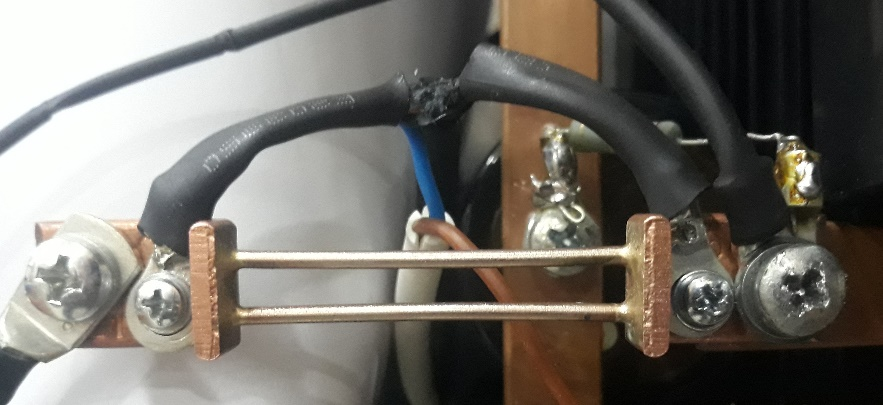
\includegraphics[width=0.94\textwidth]{deneysel/onceki_tez_sekil_5_13_sont_baglanti.jpeg}
  \caption{\SI{20}{\ampere}--\SI{60}{\milli\volt} şönt direnç bağlantısı.}
  \label{fig:deney-sont-baglanti}
\end{figure}

AA tarafta Entes EMK-01 analizörü ve 50/5 oranlı, \SI{5}{\volt\ampere}, Class~0.1 akım transformatörleri kullanılmıştır. Üç faz ve nötr hattı için dört akım transformatörü bağlanmış; faz--nötr gerilimleri, faz/nötr akımları, aktif ve reaktif güç ile toplam THD değerleri Modbus RTU üzerinden okunmuştur. Şekil~\ref{fig:deney-emk01}(a) analizörü, Şekil~\ref{fig:deney-emk01}(b) üreticinin bağlantı düzenini vermektedir.

\begin{figure}[htbp]
  \centering
  \begin{subfigure}[t]{0.43\textwidth}
    \centering
    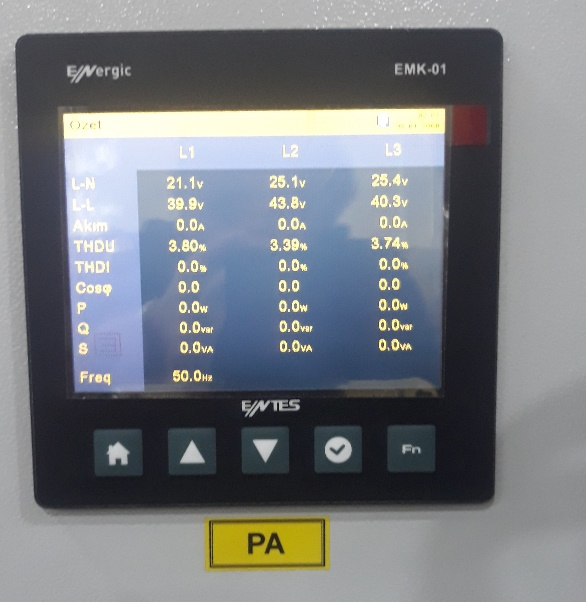
\includegraphics[width=\linewidth]{deneysel/onceki_tez_sekil_5_14a_emk01.jpeg}
    \caption{EMK-01 AA analizörü.}
  \end{subfigure}\hfill
  \begin{subfigure}[t]{0.53\textwidth}
    \centering
    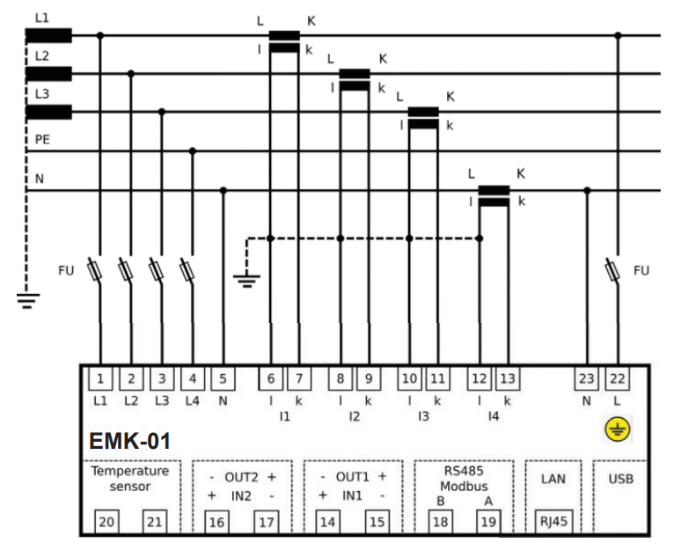
\includegraphics[width=\linewidth]{deneysel/onceki_tez_sekil_5_14b_emk01_baglanti.png}
    \caption{Üretici tarafından önerilen bağlantı şekli.}
  \end{subfigure}
  \caption{EMK-01 AA analizörü ve bağlantısı.}
  \label{fig:deney-emk01}
\end{figure}

\section{PC Ana Kumanda Yazılımı ve Veri Toplama}

PC ana kumanda yazılımı; EMK-01, AcuDC240 ve kontrol kartından RS485/Modbus RTU üzerinden veri almak, anlık değerleri grafikleştirmek ve verim hesabına temel oluşturmak amacıyla geliştirilmiştir. Şekil~\ref{fig:deney-pc-arayuzu} yazılımın arayüzünü göstermektedir. Bir veri çevrimi yaklaşık \SI{1}{\second} sürmekte; önce DA analizörü, en fazla yaklaşık \SI{50}{\milli\second} sonra AA analizörü okunmaktadır. Yapı kararlı durum eğilimleri için kullanılabilir; hızlı geçici rejimlerin tam eşzamanlı karşılaştırılması için yeterli değildir.

Haberleşme hızı cihazların izin verdiği en yüksek değer olan 38400 baud seçilmiş; veri sırası DA analizörü, AA analizörü ve kontrol kartı biçiminde kurulmuştur. Yazılımın karşılaştırma seti verim, THD, güç faktörü, faz akımı, faz--nötr gerilimi ve DA bara geriliminden oluşmaktadır. Osiloskop kanal adlarında ``kontrolör çıkışı'' ifadesi geçmektedir. Senaryo tanımlarında S1--S3 açık çevrim modülasyonla çalışır ve akım geri beslemesi yalnız S4'te bulunur (Kesim~\ref{sec:s4-kapali-cevrim}); kanal adındaki ifade, modülasyon komutu olarak okunmuştur. Donanım yazılımı belgelenmediğinden okuma, benzetim modelinin yapısına dayanmaktadır.

\begin{figure}[htbp]
  \centering
  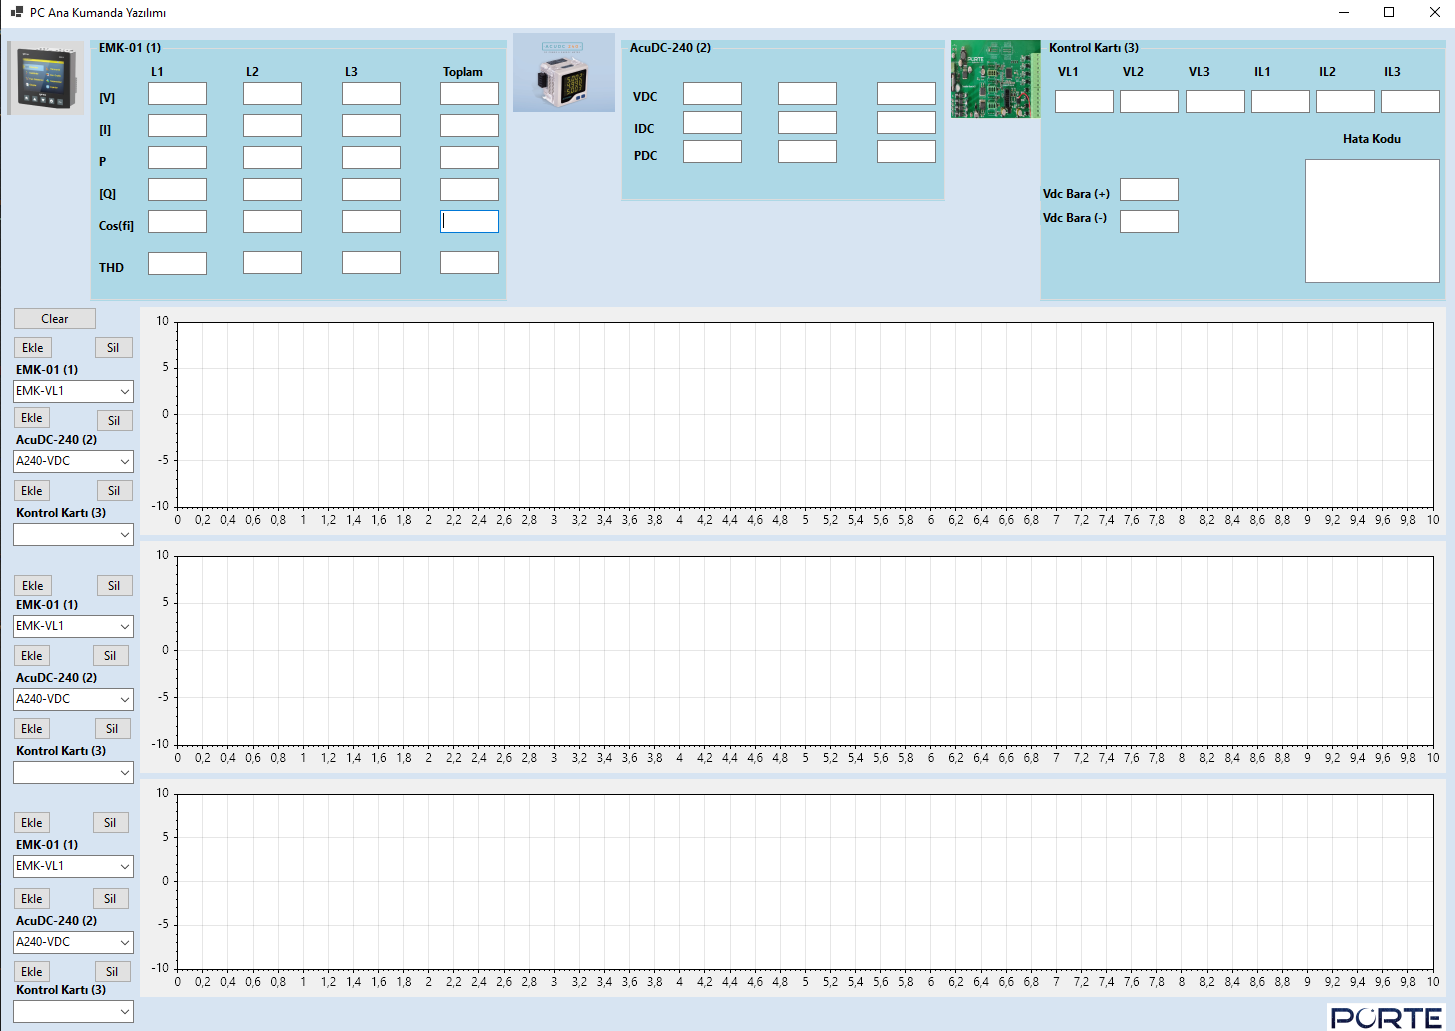
\includegraphics[width=0.98\textwidth]{deneysel/onceki_tez_sekil_5_15_pc_arayuzu.png}
  \caption{Haberleşme sistemi arayüzü.}
  \label{fig:deney-pc-arayuzu}
\end{figure}

Ortak hedef çalışma koşulu; DA bara gerilimi yaklaşık \SI{400}{\volt}, faz--nötr gerilimi yaklaşık \SI{130}{\volt}, faz akımı yaklaşık \SI{2.3}{\ampere} ve birim güç faktörüne yakın işletim olarak tanımlanmıştır. Gerçek ekran ve metin kayıtları yöntemler arasında farklı DA bara ve faz gerilimleri bulunduğunu göstermektedir. Verim, THD ve ters akım ölçütleri Eşitlik~\eqref{eq:verim-tanimi}, Eşitlik~\eqref{eq:thd-rmse-tanimlari} ve Eşitlik~\eqref{eq:ters-akim-anahtarlama-olcutleri} ile ilişkilendirilmiştir.

\section{Klasik Anahtarlama Modu Deney Kayıtları}

Klasik yöntemde bütün anahtarlar tamamlayıcı sürülmekte ve düşük akımda senkron-buck benzeri ters akım yolu açık kalmaktadır. Deney özeti yüzde 92,5 verim, yüzde 15 akım THD'si, yaklaşık \SI{2.3}{\ampere} faz akımı, \SI{120}{\volt} faz--nötr gerilimi ve \SI{430}{\volt} DA bara gerilimi bildirmektedir.

Şekil~\ref{fig:deney-klasik-pc}, PC yazılımında klasik anahtarlama sırasında elde edilen grafiklerin tamamını göstermektedir; AA/DA analizör değerleri ile güç ve THD eğilimleri aynı arayüzde izlenmektedir.

\begin{figure}[htbp]
  \centering
  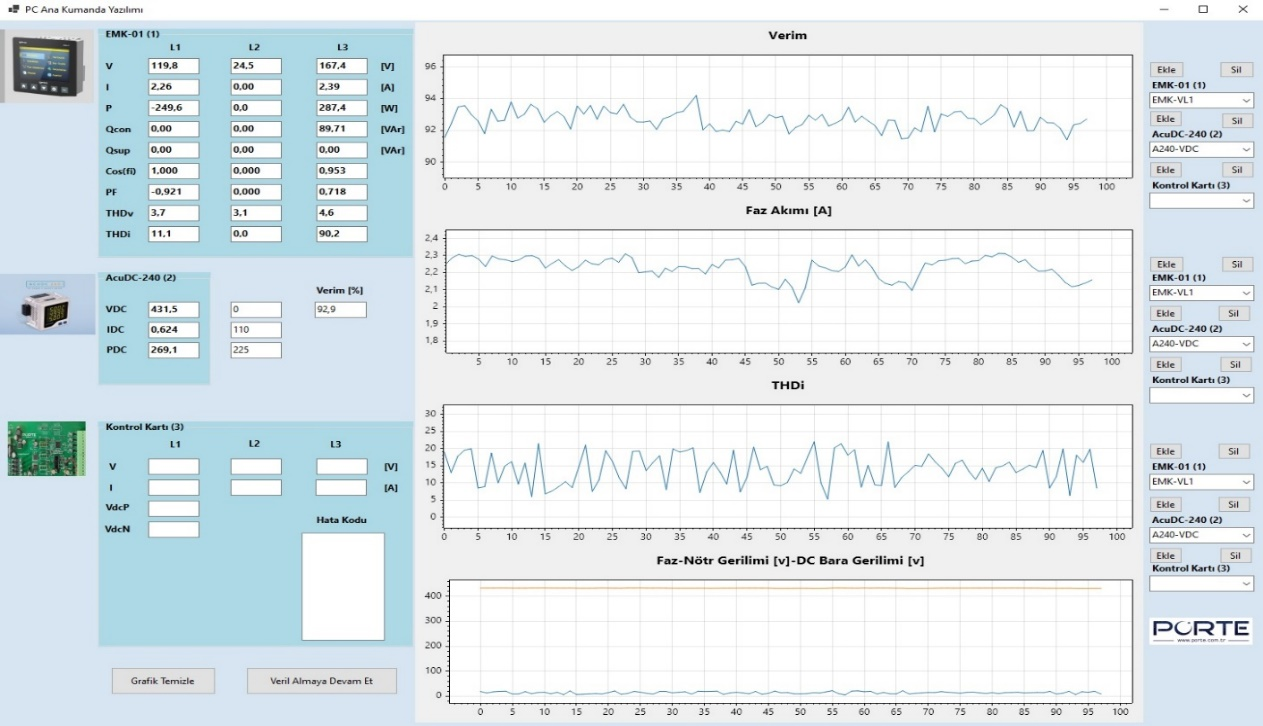
\includegraphics[width=0.98\textwidth]{deneysel/onceki_tez_sekil_5_16_klasik_pc.jpeg}
  \caption{Klasik anahtarlama sırasında PC yazılımında alınan grafikler.}
  \label{fig:deney-klasik-pc}
\end{figure}

Şekil~\ref{fig:deney-klasik-l1} üzerinde yukarıdan aşağıya kontrol işareti, şebeke gerilimi, işlemciden alınan ortalama endüktör akımı ve akım probuyla ölçülen $L_1$ akımı bulunmaktadır. Kayıt, anahtarlama dalgalanmasını ve akımın sıfır çevresindeki davranışını doğrudan göstermektedir.

\begin{figure}[htbp]
  \centering
  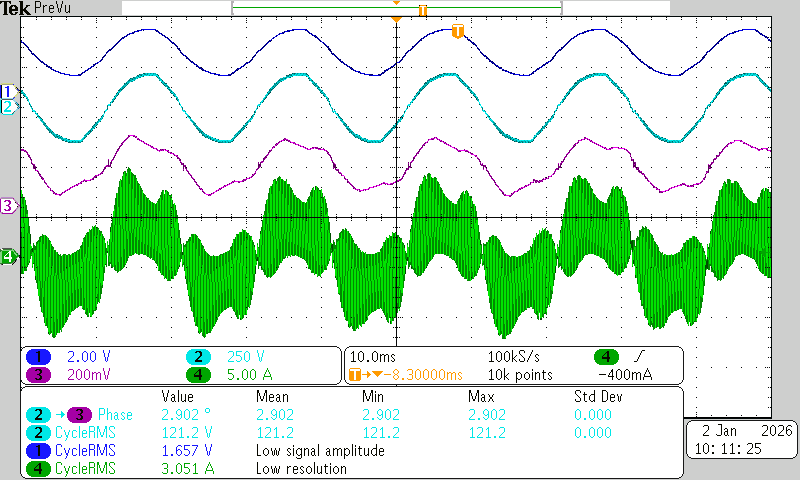
\includegraphics[width=0.94\textwidth]{deneysel/onceki_tez_sekil_5_17_klasik_l1.png}
  \caption{Klasik yöntemde kontrol işareti, şebeke gerilimi, ortalama endüktör akımı ve $L_1$ akımı.}
  \label{fig:deney-klasik-l1}
\end{figure}

Şekil~\ref{fig:deney-klasik-faz} üzerinde ilk üç kanal korunmuş, dördüncü kanalda faz akımı verilmiştir. $L_1$ akımı ile faz akımının ayrı kayıtlarda sunulması, filtre ve şebeke tarafındaki dalga biçimlerinin aynı fiziksel büyüklük olarak yorumlanmasını önlemektedir.

\begin{figure}[htbp]
  \centering
  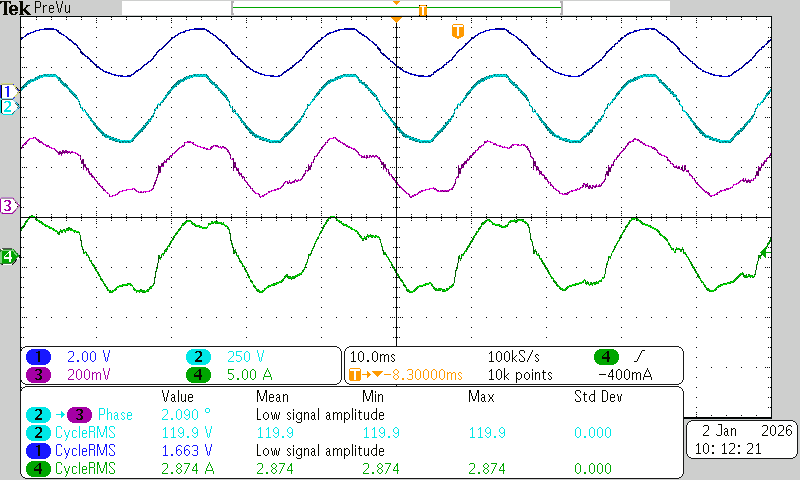
\includegraphics[width=0.94\textwidth]{deneysel/onceki_tez_sekil_5_18_klasik_faz.png}
  \caption{Klasik yöntemde kontrol işareti, şebeke gerilimi, ortalama endüktör akımı ve faz akımı.}
  \label{fig:deney-klasik-faz}
\end{figure}

\section{Nötr Anahtar Susturma Modu Deney Kayıtları}

Nötr anahtar susturma yönteminde ilgili yarım periyotta ters akım yolu kesilmekte, düşük görev oranında kesintili iletim ve üçüncü harmonik ağırlıklı akım zarfı ortaya çıkmaktadır. Deney özeti yüzde 94,2 verim, yüzde 46 akım THD'si, yaklaşık \SI{2.3}{\ampere} faz akımı, \SI{120}{\volt} faz--nötr gerilimi ve \SI{395}{\volt} DA bara gerilimi vermektedir.

\begin{figure}[htbp]
  \centering
  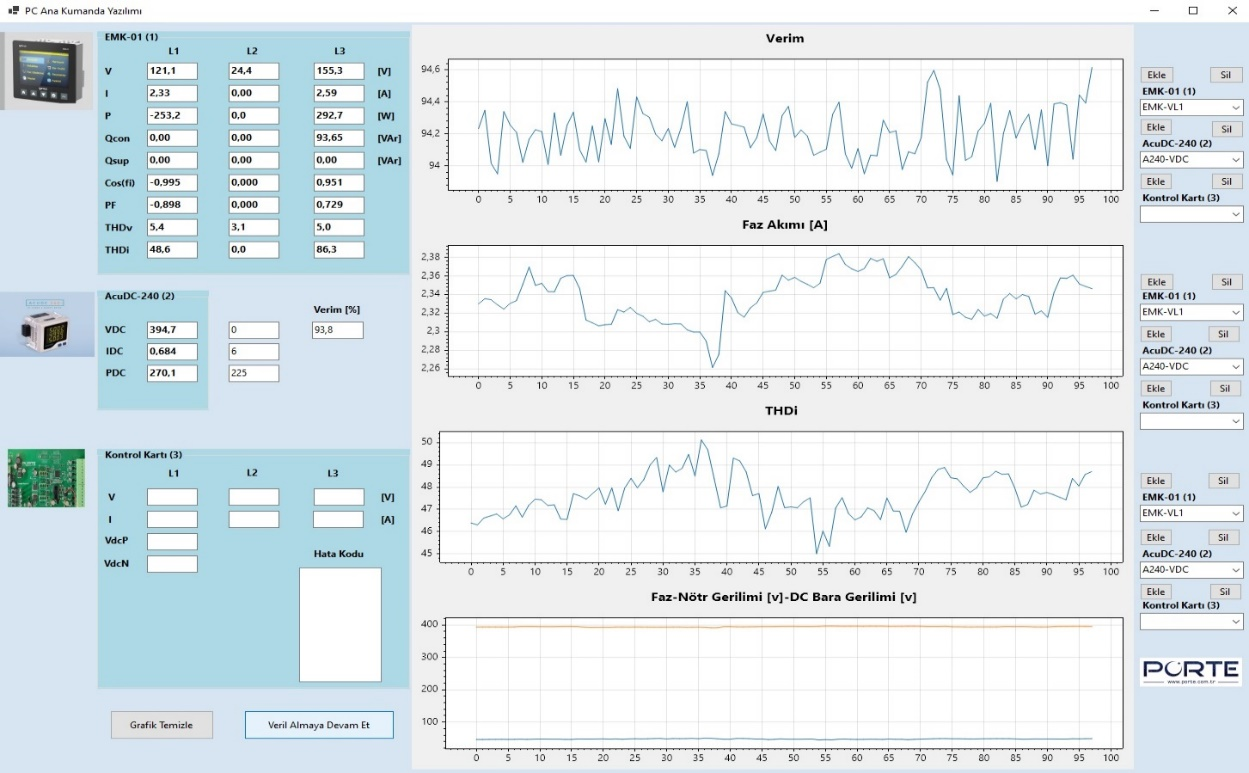
\includegraphics[width=0.98\textwidth]{deneysel/onceki_tez_sekil_5_19_susturma_pc.jpeg}
  \caption{Nötr anahtar susturma modunda PC yazılımında elde edilen grafikler.}
  \label{fig:deney-susturma-pc}
\end{figure}

Şekil~\ref{fig:deney-susturma-l1}, anahtarlamalı endüktör akımının sıfır çevresinde kesildiği aralıkları göstermektedir. Gözlenen zarf, Bölüm~\ref{chap:anahtarlama} içindeki Senaryo~2 kayıtları ve üçüncü harmonik mekanizmasıyla nitel olarak uyumludur.

\begin{figure}[htbp]
  \centering
  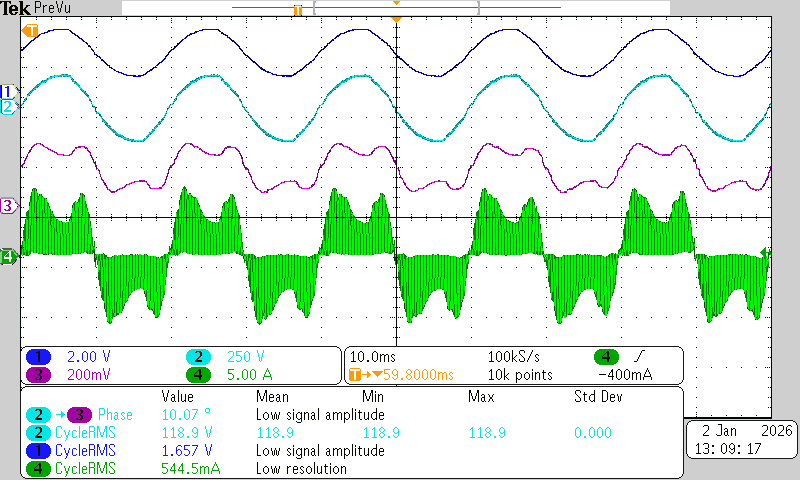
\includegraphics[width=0.94\textwidth]{deneysel/onceki_tez_sekil_5_20_susturma_l1.png}
  \caption{Susturma yönteminde kontrol işareti, şebeke gerilimi, ortalama endüktör akımı ve $L_1$ akımı.}
  \label{fig:deney-susturma-l1}
\end{figure}

Şekil~\ref{fig:deney-susturma-faz}, aynı yöntemin faz akımındaki belirgin biçim bozulmasını göstermektedir. Klasik yönteme göre farklı DA bara gerilimi kullanıldığından verim değişiminin tamamı yalnız anahtarlama yöntemine atfedilemez.

\begin{figure}[htbp]
  \centering
  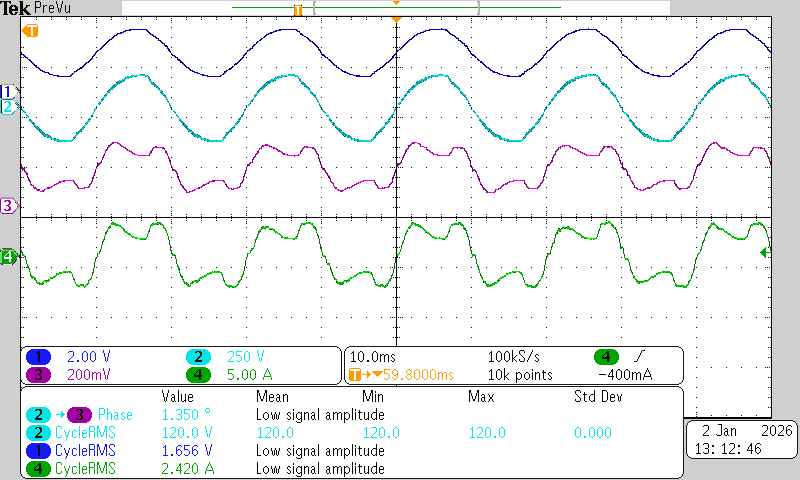
\includegraphics[width=0.94\textwidth]{deneysel/onceki_tez_sekil_5_21_susturma_faz.png}
  \caption{Susturma yönteminde kontrol işareti, şebeke gerilimi, ortalama endüktör akımı ve faz akımı.}
  \label{fig:deney-susturma-faz}
\end{figure}

\section{Susturma ve Sin\texorpdfstring{\textsuperscript{3}}{3} Modu Deney Kayıtları}

Üçüncü yöntemde nötr anahtar susturma korunmuş ve akım zarfındaki harmonik bozulmayı azaltmak amacıyla Sin\textsuperscript{3} tabanlı terim eklenmiştir. Deney özeti yüzde 94,5 verim, yüzde 14 akım THD'si, yaklaşık \SI{2.3}{\ampere} faz akımı, \SI{124}{\volt} faz--nötr gerilimi ve \SI{427}{\volt} DA bara gerilimi bildirmektedir. Benzetim modelinde terim $K_3\sin^3\theta$ biçimindedir (Bölüm~\ref{chap:sin3}); donanım yazılımı belgelenmediğinden deneydeki uygulamanın aynı biçimde olduğu kabul edilmiştir.

\begin{figure}[htbp]
  \centering
  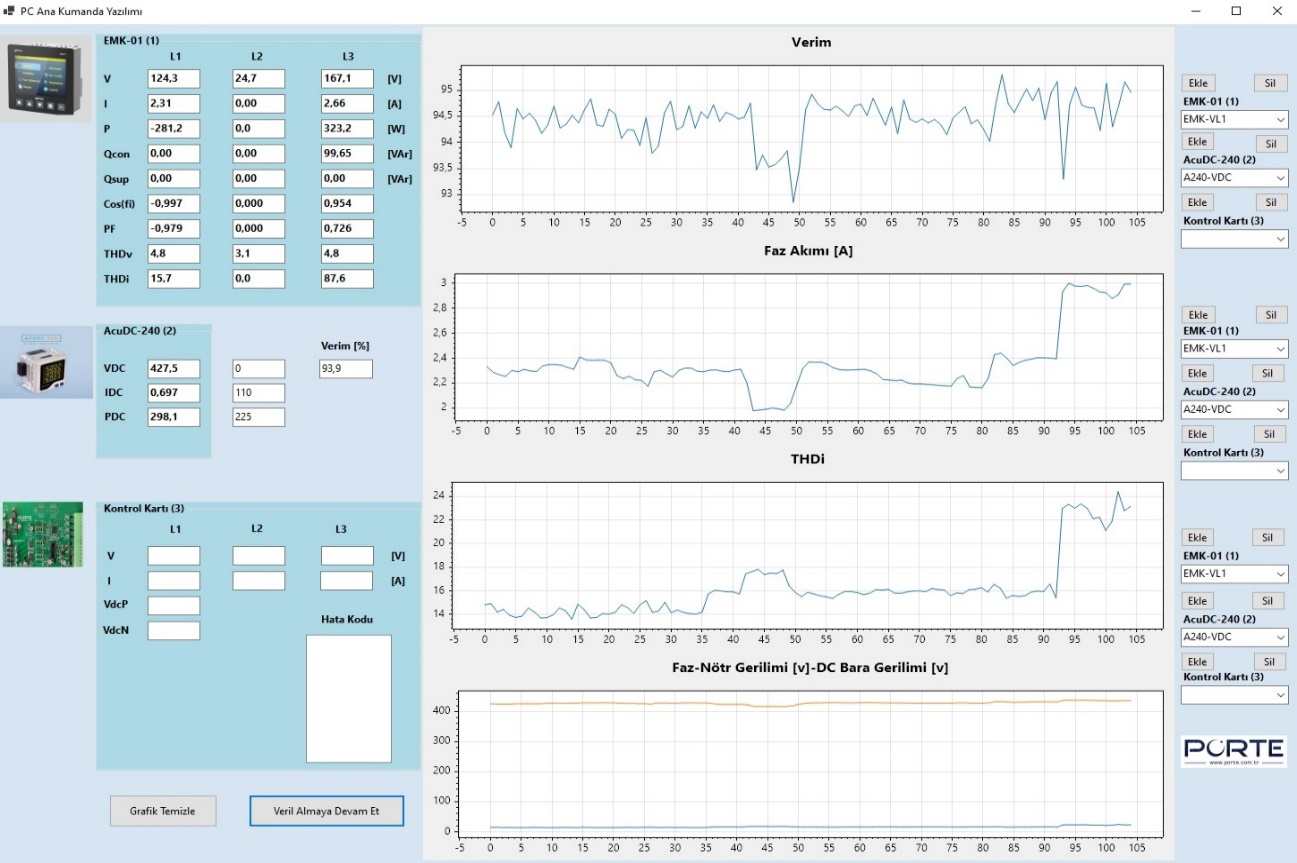
\includegraphics[width=0.98\textwidth]{deneysel/onceki_tez_sekil_5_22_sin3_pc.jpeg}
  \caption{Sin\textsuperscript{3} uygulanmış susturma modunda PC yazılımında alınan grafikler.}
  \label{fig:deney-sin3-pc}
\end{figure}

Şekil~\ref{fig:deney-sin3-l1}, susturma deneyine göre daha düzenli bir $L_1$ akım zarfı göstermektedir; nitel iyileşme, bildirilen THD azalmasıyla uyumludur.

\begin{figure}[htbp]
  \centering
  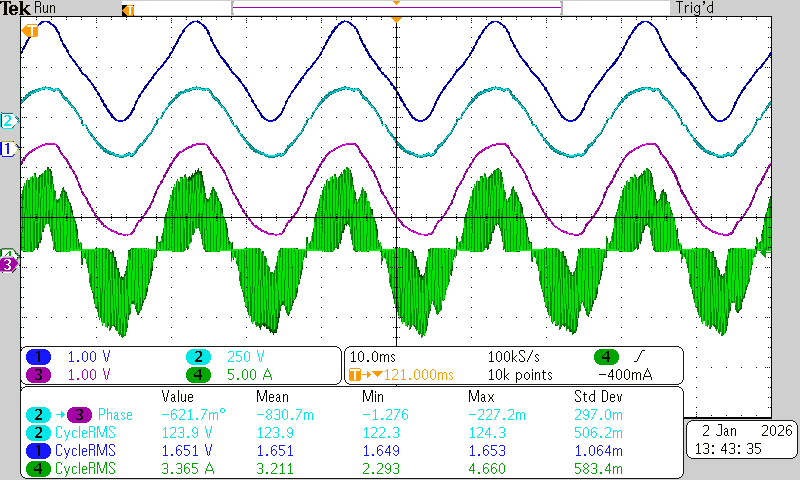
\includegraphics[width=0.94\textwidth]{deneysel/onceki_tez_sekil_5_23_sin3_l1.png}
  \caption{Sin\textsuperscript{3} uygulanmış yöntemde kontrol işareti, şebeke gerilimi, ortalama endüktör akımı ve $L_1$ akımı.}
  \label{fig:deney-sin3-l1}
\end{figure}

Şekil~\ref{fig:deney-sin3-faz}, faz akımındaki zarfın susturma yöntemine göre düzeldiğini göstermektedir. Klasik ve Sin\textsuperscript{3} deneyleri farklı DA bara ve faz gerilimlerinde yapıldığından tek değişkenli nedensel üstünlük sonucu çıkarılmamıştır.

\begin{figure}[htbp]
  \centering
  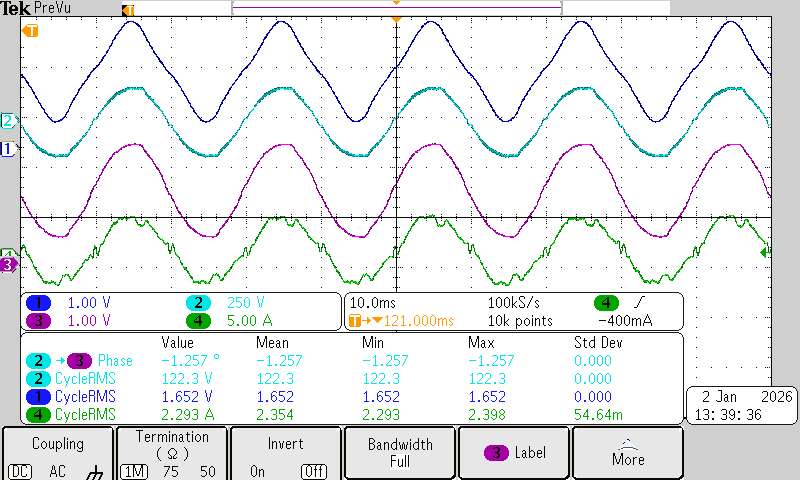
\includegraphics[width=0.94\textwidth]{deneysel/onceki_tez_sekil_5_24_sin3_faz.png}
  \caption{Sin\textsuperscript{3} uygulanmış yöntemde kontrol işareti, şebeke gerilimi, ortalama endüktör akımı ve faz akımı.}
  \label{fig:deney-sin3-faz}
\end{figure}

\section{Deney Sonuçlarının Değerlendirilmesi}

Üç yöntemin deneysel verim ve THD değerleri Tablo~\ref{tab:deney-dusuk-guc-ozeti} üzerindedir. Aynı noktalara kalibre edilen benzetim modelinin karşılık gelen değerleri, bağımsız doğrulama ölçütleriyle birlikte Kesim~\ref{sec:kalibrasyon} altında ayrı bir tabloda verilmektedir; benzetim ve deney değerleri aynı sütunda birleştirilmemiştir.

\begin{table}[htbp]
  \centering
  \caption{Üç yöntemin deneysel verim ve akım THD değerleri (deney özeti).}
  \label{tab:deney-dusuk-guc-ozeti}
  \footnotesize
  \begin{tabularx}{0.8\textwidth}{X >{\centering\arraybackslash}p{0.18\textwidth} >{\centering\arraybackslash}p{0.18\textwidth}}
    \toprule
    Yöntem & Verim & THD$_I$ \\
    \midrule
    Klasik tamamlayıcı anahtarlama & \%92,50 & \%15 \\
    Nötr anahtar susturma & \%94,20 & \%46 \\
    Susturma + Sin\textsuperscript{3} & \%94,50 & \%14 \\
    \bottomrule
  \end{tabularx}
\end{table}

Deney düzeneğindeki güç, ölçüm ve veri toplama akışı Şekil~\ref{fig:deney-olcum-zinciri} üzerinde özetlenmiştir.

\begin{figure}[htbp]
  \centering
  \begin{tikzpicture}[
    node distance=8mm and 10mm,
    block/.style={draw=blue!55!black,fill=blue!7,rounded corners,align=center,minimum height=10mm,text width=28mm,font=\small},
    meas/.style={draw=green!50!black,fill=green!8,rounded corners,align=center,minimum height=10mm,text width=28mm,font=\small},
    data/.style={draw=orange!70!black,fill=orange!10,rounded corners,align=center,minimum height=10mm,text width=30mm,font=\small},
    arr/.style={-{Latex[length=2.5mm]},thick}
  ]
    \node[block] (dc) {DA bara\\AcuDC240 + şönt};
    \node[block,right=of dc] (inv) {T-tipi evirici\\LCL filtre};
    \node[block,right=of inv] (grid) {Varyak ve\\AA şebeke};
    \draw[arr] (dc) -- node[above,font=\scriptsize] {$P_{dc}$} (inv);
    \draw[arr] (inv) -- node[above,font=\scriptsize] {$v_g,i_g$} (grid);
    \node[meas,below=of inv] (scope) {Osiloskop\\$i_{L1}$, $i_g$, $v_g$, DAC};
    \node[meas,below=of grid] (ac) {EMK-01 + CT\\$P_{ac}$, THD, PF};
    \node[meas,below=of dc] (ctrl) {Kontrol/ölçüm kartı\\ADC, PWM, FAULT};
    \draw[arr] (inv) -- (scope);
    \draw[arr] (grid) -- (ac);
    \draw[arr] (inv) -- (ctrl);
    \node[data,below=15mm of scope] (pc) {PC ana kumanda yazılımı\\RS485/Modbus RTU};
    \draw[arr] (ctrl) -- (pc);
    \draw[arr] (ac) -- (pc);
    \draw[arr] (dc) |- (pc);
    \draw[arr,dashed] (scope) -- node[right,font=\scriptsize] {ekran kaydı} (pc);
  \end{tikzpicture}
  \caption{Deney düzeneğindeki güç, ölçüm ve veri toplama akışı.}
  \label{fig:deney-olcum-zinciri}
\end{figure}

Tablo~\ref{tab:olcum-cihazlari}, kullanılan cihaz ve sensörleri doğrulama sınırlarıyla birlikte toplamaktadır. Kayıtlardaki ``Class 0,1'' ve AcuDC240 yüzde hata değerleri aynı büyüklük olarak kabul edilmemiş; osiloskop için yazılan ``300 Hz'' ifadesi model ailesiyle uyuşmadığından üretici belgesi bekleyen kayıt olarak işaretlenmiştir.

\begin{table}[htbp]
  \centering
  \caption{Ölçüm cihazları ve doğrulama sınırları.}
  \label{tab:olcum-cihazlari}
  \footnotesize
  \begin{tabularx}{\textwidth}{p{0.19\textwidth} p{0.23\textwidth} p{0.20\textwidth} X}
    \toprule
    Büyüklük & Cihaz / sensör & Bildirilen özellik & Doğrulama notu \\
    \midrule
    AA güç ve THD & Entes EMK-01 ve 50/5 oranlı, \SI{5}{\volt\ampere} akım transformatörleri & Class 0.1 & Kalibrasyon belgesi bağımsız olarak mevcut değildir. \\
    DA güç & Accuenergy AcuDC240 ve \SI{20}{\ampere}/\SI{60}{\milli\volt} şönt & Akım/gerilim yüzde 0,2; güç/enerji yüzde 0,5 & ``Class 0,1'' ifadesiyle uyuşmazlık üretici belgesiyle kesinleştirilecektir. \\
    Hızlı akım & Tektronix TCP0150 & \SI{150}{\ampere}, \SI{20}{\mega\hertz} & Prob oranı ham osiloskop dosyasıyla doğrulanacaktır. \\
    Hızlı gerilim & Tektronix THDP0200 & \SI{1500}{\volt}, \SI{200}{\mega\hertz} & Kanal zayıflatması ve ortak-mod sınırı ham kayıtla doğrulanacaktır. \\
    Osiloskop & Tektronix DPO3034 & Kayıtta ``300 Hz, 2,5 GS/s'' & ``300 Hz'' ifadesi model veri sayfasıyla uyuşmadığından bant genişliği doğrulanmalıdır. \\
    Faz/LCL akımı & HLSR 20-P/SP33 & \SI{23}{\milli\volt\per\ampere}; \SI{39.9}{\ampere} RMS hesap sınırı & Kazanç ve ADC ölçekleme katsayıları kontrol koduyla doğrulanacaktır. \\
    Gerilim ölçümü & AMC1200 tabanlı izole kart & Kazanç 8; \SI{2.6}{\volt} ADC aralığı & Direnç oranı ve kanal kalibrasyonu şemadan doğrulanacaktır. \\
    \bottomrule
  \end{tabularx}
\end{table}

Üç yöntemin çalışma koşulları Tablo~\ref{tab:deney-kosullari} üzerinde karşılaştırılmıştır. Yöntemler tam olarak aynı DA bara ve faz gerilimlerinde çalıştırılmadığından, verim sıralaması tek değişkenli bir yöntem karşılaştırması değildir.

\begin{table}[htbp]
  \centering
  \caption{Üç yöntem için bildirilen çalışma koşulları.}
  \label{tab:deney-kosullari}
  \footnotesize
  \begin{tabularx}{\textwidth}{p{0.21\textwidth} *{3}{>{\centering\arraybackslash}X} X}
    \toprule
    Büyüklük & Klasik & Nötr susturma & Susturma+Sin\textsuperscript{3} & Yorum \\
    \midrule
    Faz akımı & \SI{2.3}{\ampere} & \SI{2.3}{\ampere} & \SI{2.3}{\ampere} & Düşük güç noktası; anma testi değildir. \\
    Faz--nötr gerilimi & \SI{120}{\volt} & \SI{120}{\volt} & \SI{124}{\volt} & Yöntemler tam aynı gerilimde değildir. \\
    DA bara gerilimi & \SI{430}{\volt} & \SI{395}{\volt} & \SI{427}{\volt} & Yöntemler tam aynı bara koşulunda değildir. \\
    Analizörün $\cos\varphi$ göstergesi & $-0{,}990$--$1{,}000$ & $-0{,}995$ & $-0{,}997$ & Temel bileşen yer değiştirme faktörüdür; işaret kuralı belgelenmemiştir (Kesim~\ref{sec:kalibrasyon}). \\
    \bottomrule
  \end{tabularx}
\end{table}

Deney özet değerleri ile PC ekranlarında görünen anlık değerler de birebir aynı değildir; Tablo~\ref{tab:deney-metin-ekran-karsilastirma} farkları görünür kılmaktadır. Ekran değeri, görselde okunabilen tek anlık görüntüdür; özet değeri deney raporundaki sayıdır. Ham kayıtlar bulunmadan farkların ortalama, medyan, seçilmiş an veya farklı faz sonucu olup olmadığı belirlenemez; tablo bir hata düzeltme tablosu değil, kaynak içi tutarlılık denetimidir.

\begin{table}[htbp]
  \centering
  \caption{Deney özeti ile PC ekranlarında okunabilen anlık değerlerin karşılaştırılması.}
  \label{tab:deney-metin-ekran-karsilastirma}
  \footnotesize
  \begin{tabularx}{\textwidth}{p{0.21\textwidth} p{0.16\textwidth} >{\centering\arraybackslash}X >{\centering\arraybackslash}X X}
    \toprule
    Yöntem & Büyüklük & Özet & PC ekranı & Farkın durumu \\
    \midrule
    Klasik & Verim & \%92,5 & \%92,9 & Ortalama/anlık ayrımı doğrulanamadı. \\
    Klasik & THD$_i$ & \%15 & \%11,1 & Analiz penceresi ve ortalama yöntemi eksik. \\
    Klasik & $V_{dc}$ & \SI{430}{\volt} & \SI{431.5}{\volt} & Yakın değerler. \\
    \midrule
    Nötr susturma & Verim & \%94,2 & \%93,8 & Ortalama/anlık ayrımı doğrulanamadı. \\
    Nötr susturma & THD$_i$ & \%46 & \%48,6 & Aynı yüksek bozulma eğilimi; sayısal fark açık. \\
    Nötr susturma & $V_{dc}$ & \SI{395}{\volt} & \SI{394.7}{\volt} & Yakın değerler. \\
    \midrule
    Susturma+Sin\textsuperscript{3} & Verim & \%94,5 & \%93,9 & Ortalama/anlık ayrımı doğrulanamadı. \\
    Susturma+Sin\textsuperscript{3} & THD$_i$ & \%14 & \%15,7 & Aynı iyileşme eğilimi; sayısal fark açık. \\
    Susturma+Sin\textsuperscript{3} & $V_{dc}$ & \SI{427}{\volt} & \SI{427.5}{\volt} & Yakın değerler. \\
    \bottomrule
  \end{tabularx}
\end{table}

Deneysel kayıtlar yalnız yaklaşık \SI{2.3}{\ampere} düşük güç noktasını belgelemektedir. Orta ve anma akımında aynı denetim yapısının davranışı S4 benzetim taramasıyla (Kesim~\ref{sec:s4-kapali-cevrim}) incelenmiştir; Tablo~\ref{tab:deney-juri-durum}, güç bölgelerine göre deneysel ve benzetim kanıtını ayırmaktadır.

\begin{table}[htbp]
  \centering
  \caption{Doğrulamanın güç bölgelerine göre kanıt düzeyi.}
  \label{tab:deney-juri-durum}
  \small
  \begin{tabularx}{\textwidth}{p{0.17\textwidth} X X p{0.21\textwidth}}
    \toprule
    Çalışma bölgesi & Deneysel kanıt & Benzetim kanıtı & Tezdeki kullanım \\
    \midrule
    Düşük güç (\SI{2.3}{\ampere}) & Üç yönteme ait PC ve osiloskop ekranları; deney özeti & S1--S3 kalibre benzetimi (Tablo~\ref{tab:kalibrasyon-karsilastirma}); S4 \SI{2.3}{\ampere} koşuları & Destekleyici deneysel kanıt ve kalibre benzetim \\
    Orta güç (\SI{10}{\ampere}) & Kayıt yok & S4 P, PI, PIR koşuları (Tablo~\ref{tab:s4-tarama}) & Yalnız benzetim bulgusu \\
    Anma (\SI{25}{\ampere}) & Kayıt yok & S4 P, PI, PIR koşuları; büyütülmüş DA bara (Tablo~\ref{tab:s4-tarama}) & Yalnız benzetim bulgusu \\
    Geçici rejim & Kayıt yok & S4 \SI{10}{\ampere}$\rightarrow$\SI{25}{\ampere} basamağı (Tablo~\ref{tab:s4-basamak}) & Yalnız benzetim bulgusu \\
    \bottomrule
  \end{tabularx}
\end{table}

Orta ve anma gücünde deney yapılamamasının iki nedeni vardır. Birincisi, laboratuvar şebeke bağlantısının varyak üzerinden yaklaşık \SI{120}{\volt} ile sınırlı olmasıdır; anma gücü ifadeleri donanımın tasarım hedefi olarak kalmaktadır. İkincisi, deney donanımının DA bara kapasitörleri \SI{25}{\ampere} faz akımında bara orta noktasını tutamamaktadır (Kesim~\ref{sec:s4-kapali-cevrim}). Şebeke gerilimi ve DA bara sınırları nedeniyle orta ve anma akımı sonuçları deneyle doğrulanmamış benzetim bulgusu olarak raporlanmaktadır. Deneysel verimin belirsizliği için yalnız bir alt sınır verilebilir: DA analizörünün bildirilen yüzde 0,5 güç toleransı, birleşik belirsizliğin $u_{\eta}=\eta\sqrt{(u_{P_{ac}}/P_{ac})^2+(u_{P_{dc}}/P_{dc})^2}$ ilk yaklaşımında AA tarafı katkısı olmadan da \%94 verimde yaklaşık $\pm0{,}5$ puan verir. S2 ile S3 arasındaki 0,3 puanlık deneysel verim farkı belirsizlik alt sınırının içindedir.

\subsection{Deney Özet Tablosunun Sayısal Denetimi}

17.08.2026 tarihli çalışma kitabının gerçek uygulama alanı Senaryo~1--3 için tek satırlık özetler içermekte, ham zaman serisi veya tekrar koşusu vermemektedir. Tablo~\ref{tab:gelen-excel-senaryolar}, hücrelerdeki değerleri değiştirmeden ve $\eta_{VI}=100P_{\mathrm{out}}/(V_{\mathrm{dc}}I_{\mathrm{dc}})$ bağımsız hesabını ayrıca göstererek kaynağın izini korumaktadır.

\begin{table}[htbp]
  \centering
  \caption{Deney özet tablosundaki değerler ve DA giriş çarpımından yeniden hesaplanan verim.}
  \label{tab:gelen-excel-senaryolar}
  \footnotesize
  \begin{tabularx}{\textwidth}{c r r r r r r r}
    \toprule
    Senaryo & $V_{dc}$ (V) & $I_{dc}$ (A) & $V_{ac}$ (V RMS) & $I_{faz}$ (A) & $P_o$ (W) & THD (\%) & $\eta_{VI}$ (\%) \\
    \midrule
    1 & 431,5 & 0,624 & 119,8 & 2,26 & 249,6 & 15 & 92,700 \\
    2 & 395,0 & 0,684 & 121,0 & 2,33 & 253,2 & 47 & 93,715 \\
    3 & 427,5 & 0,697 & 124,3 & 2,31 & 281,2 & 14 & 94,373 \\
    \bottomrule
  \end{tabularx}
\end{table}

Bildirilen verimler sırasıyla \%92,5, \%94,2 ve \%94,5'tir; yeniden hesaplanan değerlerle farklar yaklaşık $-0{,}20$, $+0{,}48$ ve $+0{,}13$ yüzde puandır. Farkların yuvarlama, farklı ortalama penceresi veya ek kayıp teriminden kaynaklanıp kaynaklanmadığı ham güç örnekleri olmadan çözülemez. Kitabın benzetim satırları aynı temel sayıları tekrar etmekte, bağımsız Simulink çıktısı ya da ham iz sağlamamaktadır; tablo yalnız deneysel özet olarak kullanılmış, benzetim doğrulaması sayılmamıştır. Benzetim karşılaştırması, Kesim~\ref{sec:kalibrasyon} altında model koşularından yapılmıştır.

\section{Benzetim Modelinin Deney Özetine Kalibrasyonu}
\label{sec:kalibrasyon}

Deney özeti ile benzetim modelinin karşılaştırılabilmesi için S1--S3 benzetim modelleri deney özetinin çalışma noktalarına kalibre edilmiştir. Kesimin amacı, modelin deneyin hangi büyüklüklerini hangi hatayla yeniden ürettiğini göstermek ve kalibre benzetimi deney bulgusundan ayrı tutmaktır. Taban modeller, Kesim~\ref{sec:model-dogrulama-duzeltme} altında özetlenen düzeltmelerin uygulandığı S1, S2 ve S3 modelleridir. Kalibre değerler Tablo~\ref{tab:sistem-parametreleri} içinde ``Kalibre'' türüyle, parametre dosyasındaki ilk değerleri parantez içinde olmak üzere verilmiştir; S4 ileri beslemesi kalibre S3 değerlerini kullanır.

\subsection{Yöntem}

Devre, yarı iletken ve filtre parametreleri kalibrasyonda değiştirilmemiştir. Her senaryoda yalnız iki serbest değişken vardır: modülasyon genlik ölçeği ($K_{1x}$; S3'te $K_3/K_1$ oranı sabit tutularak $K_{13}$ ile $K_{33}$ birlikte) ve şebekeye göre referans fazı $\varphi_x$. İki serbest değişken iki hedefe ayarlanmıştır: etkin güç $P_{\mathrm{ac}}$ deney değerinin $\pm$\%1'i içinde, temel bileşen reaktif gücünün büyüklüğü $|Q_1|$ ise deneydeki $\cos\varphi$ okumasının yuvarlama bandı içinde tutulmuştur. AA çıkış akımı $I_{\mathrm{ac}}$, verim, DA güç ve akımı, $|\cos\varphi_1|$, güç faktörü ve akım THD'si kalibre edilmemiştir ve bağımsız doğrulama ölçütüdür. THD hedefi olarak deney özetinin \%15, \%47 ve \%14 değerleri alınmış, THD birincil ölçütler olan $P_{\mathrm{ac}}$, $I_{\mathrm{ac}}$ ve verimin ardından ikincil ölçüt olarak değerlendirilmiştir.

\textbf{Reaktif güç işareti ve ölçüm noktası.} Benzetimde güç büyüklükleri evirici çıkış uçlarında, yani EMC süzgecinden sonra ve $L_2$ ile temsil edilen şebeke ve varyak eşdeğerinden önce ölçülmektedir; nokta, deneyde AA analizörünün bağlı olduğu yaklaşık \SI{120}{\volt} tarafına karşılık gelir. İşaret kuralı üreticidir: evirici$\rightarrow$şebeke yönü pozitiftir, $Q_1>0$ akımın gerilimin gerisinde olduğu ve eviricinin şebekeye reaktif güç verdiği durumdur. Benzetimdeki pozitif $Q_1$'in kaynağı filtre kapasitörüdür. Deney özetindeki reaktif güç ölçülmemiş, $Q_o=P_o\tan(\arccos\cos\varphi)$ ile hesaplanmıştır ve eksi işareti analizörün $\cos\varphi$ göstergesinden gelir. Analizörün yön ve öncü/artçı kuralı belgelenmediğinden işaret yorumlanmamış, karşılaştırma büyüklükler ($|Q_1|$, $|\cos\varphi_1|$) üzerinden yapılmıştır. Deneydeki $\cos\varphi$, temel bileşen yer değiştirme faktörüdür ($\cos\varphi_1$) ve toplam güç faktöründen ($\mathrm{PF}=P/(V_{\mathrm{rms}}I_{\mathrm{rms}})$) ayrı raporlanmıştır. Üç basamaklı $\cos\varphi$ okuması $|Q_1|$ için S1'de 0--7,9~var, S2'de 24,1--26,7~var, S3'te 19,9--23,6~var bandı verir; şebeke gerilimi okumasının \SI{0.1}{\volt} çözünürlüğü $|Q_1|$'de yaklaşık $\pm12$~var belirsizlik doğurduğundan $|Q_1|$ uyumsuzluğu tek başına modeli reddettirmez. Deney iki işaret dalını ayırt edemediğinden her senaryoda kalibrasyonsuz modelin dalı ($Q_1>0$) korunmuştur.

\textbf{Köprünün yumuşak kaynak davranışı.} İlk kalibrasyon adımları, evirici köprüsünün temel bileşen geriliminin modülasyonla bire bir kaymadığını göstermiştir. Köprü, koşulardan ölçülen bir Thevenin eşdeğeriyle temsil edildiğinde iç empedansın büyüklüğü S1'de \SI{1.67}{\ohm}, S2'de \SI{28.7}{\ohm}, S3'te \SI{13.7}{\ohm} çıkmıştır. S1'deki değer, tamamlayıcı anahtarlamada akım dalgalanmasının her periyotta sıfırı kesmesiyle \SI{1}{\micro\second} ölü zamanın akıma bağlı gerilim hatası üretmesinden kaynaklanır; kaba ölü zaman kestirimi de yaklaşık \SI{1.7}{\ohm} verir. S2 ve S3'te köprü, son \SI{20}{\milli\second}'lik pencerenin \%12,4 ve \%22,6'sında süreksiz iletimdedir; susturmalı köprü düşük akımda akım kaynağına yaklaşır ve senkron olmayan buck eşdeğeriyle aynı davranışı gösterir (Kesim~\ref{sec:dusuk-akim-modelleme}). Thevenin empedansı LCL ağının \SI{50}{\hertz} empedansından büyük olduğundan etkin güç esas olarak genlikle, reaktif güç esas olarak fazla değişmektedir. İki değişken birbirini etkilediği için hedefler, koşulardan öğrenilen ampirik Jacobian ile iki boyutlu Newton yinelemesiyle birlikte çözülmüştür; S1 ve S2'de dört, S3'te altı kalibrasyon koşusu gerekmiştir.

\subsection{Kalibrasyon sonucu ve bağımsız karşılaştırma}

Kalibrasyon S1'de genliği değiştirmemiş (\%0,0003), fazı $+0{,}074^{\circ}$ kaydırmıştır; parametre dosyasındaki genlik deneyin etkin gücünü \%0,96 içinde zaten vermektedir ve faz düzeltmesi yalnız $|Q_1|$'i bant içine taşır. S2'de genlik \%3,3, S3'te \%1,5 azalmış, fazlar $+0{,}11^{\circ}$ ve $+0{,}66^{\circ}$ kaymıştır. Genlik belirsizliği deney toleransının ölçülen duyarlılıklara bölünmesiyle S1'de $\pm$\%0,025, S2'de $\pm$\%0,4, S3'te $\pm$\%0,2; faz belirsizliği sırasıyla $\pm0{,}05^{\circ}$, $\pm0{,}4^{\circ}$ ve $\pm0{,}5$--$1^{\circ}$ bulunmuştur. S2 ve S3 fazları faz belirsizliğinin içindedir ve fiziksel bir gecikme olarak yorumlanmamıştır. S2 ve S3'teki genlik azalması, yaklaşık \SI{50}{\micro\second}'lik ortalama iletim süresinde darbe başına 0,7--\SI{1.6}{\micro\second} kısalmaya eşdeğerdir; değer, modelde bulunmayan sürücü ve anahtar gecikmelerinin darbe genişliğinden yediği süre düzeyindedir. Yorum bir varsayımdır ve donanım kaydıyla doğrulanmamıştır.

\begin{table}[htbp]
  \centering
  \caption{Deney özeti ile kalibre benzetim modelinin karşılaştırılması. İlk iki satır kalibrasyon hedefidir; diğer satırlar kalibre edilmemiştir ve bağımsız karşılaştırmadır. Fark: \% göreli, ``p'' yüzde puan.}
  \label{tab:kalibrasyon-karsilastirma}
  \scriptsize
  \setlength{\tabcolsep}{2.6pt}
  \begin{tabular}{@{}l ccc ccc ccc@{}}
    \toprule
    & \multicolumn{3}{c}{S1 Klasik} & \multicolumn{3}{c}{S2 Susturma} & \multicolumn{3}{c}{S3 Susturma + Sin\textsuperscript{3}} \\
    \cmidrule(lr){2-4}\cmidrule(lr){5-7}\cmidrule(lr){8-10}
    Büyüklük & Deney & Benzetim & Fark & Deney & Benzetim & Fark & Deney & Benzetim & Fark \\
    \midrule
    $P_{\mathrm{ac}}$ (W) & 249,6 & 247,21 & $-$\%0,96 & 253,2 & 253,80 & $+$\%0,24 & 281,2 & 279,90 & $-$\%0,46 \\
    $|Q_1|$ (var) & 0--7,9 & 1,93 & bantta & 24,1--26,7 & 24,43 & bantta & 19,9--23,6 & 21,41 & bantta \\
    \midrule
    $I_{\mathrm{ac}}$ (A) & 2,26 & 2,218 & $-$\%1,8 & 2,33 & 2,416 & $+$\%3,7 & 2,31 & 2,279 & $-$\%1,4 \\
    $\eta$ (\%) & 92,5 & 91,15 & $-$1,35 p & 94,2 & 93,93 & $-$0,27 p & 94,5 & 94,25 & $-$0,25 p \\
    $P_{\mathrm{dc}}$ (W) & 269,26 & 271,21 & $+$\%0,7 & 270,18 & 270,19 & $+$\%0,004 & 297,97 & 296,97 & $-$\%0,34 \\
    $I_{\mathrm{dc}}$ (A) & 0,624 & 0,6286 & $+$\%0,7 & 0,684 & 0,6841 & $+$\%0,02 & 0,697 & 0,6947 & $-$\%0,32 \\
    THD$_I$ (\%) & 15 & 39,5 & $+$24,5 p & 47 & 56,7 & $+$9,7 p & 14 & 14,8 & $+$0,8 p \\
    $|\cos\varphi_1|$ & 1,000 & 0,99997 & $\approx0$ & 0,995 & 0,99538 & $+$0,0004 & 0,997 & 0,99708 & $+$0,0001 \\
    PF & 0,922 & 0,929 & $+$\%0,8 & 0,898 & 0,867 & $-$\%3,4 & 0,979 & 0,987 & $+$\%0,8 \\
    \bottomrule
  \end{tabular}
\end{table}

Tablo~\ref{tab:kalibrasyon-karsilastirma}, kalibre benzetimin deney özetiyle karşılaştırmasını vermektedir. Etkin güç ve reaktif güç büyüklüğü iki serbest değişkenle ayarlandığından ilk iki satırdaki uyum bir doğrulama değildir; doğrulama yalnız kalibre edilmeyen satırlardadır.

\textbf{S3.} Kalibre model deneyin AA akımını $-$\%1,4, verimini $-0{,}25$ puan, akım THD'sini $+0{,}8$ puan ve DA gücünü $-$\%0,3 hatayla yeniden üretmektedir. THD kalibre edilmemiştir: kalibrasyon öncesinde \%10,9 olan değer kalibrasyon sonrasında \%14,8 olmuştur (deney \%14). Sonuç, susturmalı çalışmanın düşük akımdaki dalga biçimi bozulmasının modelde doğru büyüklükte olduğunu gösteren en güçlü bağımsız kanıttır.

\textbf{S2.} Kalibre model DA gücünü ve DA akımını \%0,02 içinde, verimi $-0{,}27$ puan hatayla yeniden üretmektedir. AA akımı ise $+$\%3,7, THD $+9{,}7$ puan yüksektir; güç faktöründeki $-$\%3,4 fark aynı farkın sonucudur. Model S2'de deneyden daha bozuk bir akım vermektedir. İki serbest değişken etkin ve reaktif güce ayrıldığından fark kalibrasyonla kapanmaz. Olası kaynaklar, sıfır geçişi çevresindeki süreksiz iletim ayrıntısını belirleyen ve modelde bulunmayan IGBT çıkış kapasitesi ile sürücü gecikmeleri ve diyot toparlanma parametreleridir; kaynak ayrıştırılmamıştır.

\textbf{S1.} Kalibre model AA akımını $-$\%1,8, verimi $-1{,}35$ puan, DA gücünü $+$\%0,7 hatayla yeniden üretmektedir. Verim farkı, modelde \SI{24.0}{\watt}, deneyde \SI{19.7}{\watt} kayba karşılık gelir ve S1 için kayıp ayrıştırması yapılmamıştır. THD farkı ($+24{,}5$ puan) deney satırının iç tutarsızlığıyla birlikte okunmalıdır: deneyin $P/(VI)=0{,}922$ değeri $\cos\varphi_1=1$ ile ancak yaklaşık \%42 THD ile tutarlıdır; \%15 THD ile güç faktörü 0,989 olurdu. Modelin güç faktörü (0,929) deneyle \%0,8 içinde, THD'si \%39,5'tir. Model, deney satırındaki güç, gerilim ve akımla tutarlıdır; \%15 THD girdisiyle tutarlı değildir.

\textbf{Senaryo sıralaması.} Verim sıralaması S1 $<$ S2 $<$ S3, modelde ve deneyde aynıdır. S1$\rightarrow$S3 verim artışı modelde $+3{,}10$, deneyde $+2{,}0$ puan; S1$\rightarrow$S2 artışı modelde $+2{,}78$, deneyde $+1{,}7$ puandır. Fark esas olarak S1 verimindeki $-1{,}35$ puanlık sapmadan gelmektedir.

\textbf{Belirsizlik ve sınırlar.} Kararlı durum değerleri \SI{0.1}{\second} benzetimin son şebeke periyodundan alınmıştır. S2 ve S3'te son periyot ile 0,08--\SI{0.10}{\second} ortalaması arasında DA güçte 0,4--\SI{0.5}{\watt}, verimde 0,1 puana varan fark vardır; fark, verim karşılaştırmasının benzetim tarafı belirsizliğidir. Kalibre benzetim sonuçları deney bulgusu değildir; ``model, deneyin büyüklüğünü belirtilen hatayla yeniden üretmektedir'' biçiminde okunmalıdır. S2'nin AA akımı ve THD farkı, S1 deney satırının THD tutarsızlığı ve S1 verim farkı Bölüm~\ref{chap:sonuc} içinde sınırlılık olarak yer almaktadır.

\section{Bölüm Sonucu}

Deney düzeneği; T-tipi güç katı, faz modülleri, kontrol, tampon ve sürücü kartları, gerilim ve akım ölçüm devreleri, koruma devresi, AA ve DA analizörleri, şönt bağlantısı, PC yazılımı ve üç yönteme ait ekran kayıtlarıyla belgelenmiştir. Deney protokolü, ham kayıtlar ve tekrarlar mevcut olmadığından deney sonuçları ekran ve özet tablosu düzeyinde destekleyici kanıttır.

Üç yönteme ait kayıtlar, nötr susturmanın düşük güçte verimi artırırken harmonik bozulmayı büyüttüğü, Sin\textsuperscript{3} teriminin ise susturma kaynaklı bozulmayı azalttığı mekanizmasını nitel olarak desteklemektedir. Etkin ve reaktif güce kalibre edilen benzetim modeli, S3'te deneyin AA akımını \%1,4, verimini 0,25 puan ve kalibre edilmemiş akım THD'sini 0,8 puan içinde yeniden üretmekte ve deneyin verim sıralamasını korumaktadır; S2'de akım bozulmasını fazla, S1'de verimi düşük vermektedir. Özet ile ekran değerleri arasındaki farklar, yöntemler arasındaki DA bara ve şebeke gerilimi değişimi ve analizörün işaret kuralının belgelenmemesi açıkça gösterilmiştir. Orta ve anma akımı yalnız S4 benzetimiyle incelenmiştir; ortak koşullu ve anma gücünde deney yapılmamıştır.

\chapter{GT-TİPİ YENİDEN YAPILANDIRILABİLİR ENERJİ DEPOLAMA MİMARİSİ}
\label{chap:gttipi}

Önceki bölümlerde üç seviyeli T-tipi dönüştürücünün düşük güç davranışı, ters akım dolaşımı, nötr anahtar susturma yöntemi, Sin\textsuperscript{3} tabanlı ileri besleme kompanzasyonu ve mevcut deney düzeneği incelenmiştir. Düşük güç incelemesi, anma gücü tasarım hedefi \SI{20}{\kilo\volt\ampere}--\SI{25}{\kilo\watt} olan evirici altyapısına ve erişilebilen düşük güç kayıtlarına dayanmaktadır. GT-tipi mimari ise aynı deney düzeneğinin doğrudan büyütülmüş sürümü değildir; proje başvuru formunda tanımlanan \SI{100}{\kilo\watt} hedefli, değiştirilmiş T-tipi güç katı ile aktif batarya yönetimini bir araya getiren ayrı bir tasarım katmanıdır \citep{Arifoglu2023Basvuru}. İki katman birbirinin yerine geçmez: T-tipi evirici, ölçüm, koruma ve düşük güç anahtarlama birikimi Bölüm~\ref{chap:sistem}--\ref{chap:deney} içinde korunmuş; GT-tipi mimari, şebeke arayüzü, izole şarj kolları, batarya bazlı kontrol ve yeniden yapılandırılabilir deşarj dizisini aynı sistem sınırında ilişkilendiren sonraki tasarım katmanı olarak ayrılmıştır.

``GT-tipi'' adı, tezde \emph{geliştirilmiş/değiştirilmiş T-tipi} enerji depolama mimarisini belirtmek için kullanılan proje içi bir adlandırmadır; literatürde standartlaşmış bağımsız bir çok seviyeli dönüştürücü ailesi değildir. Mimari; T-tipi/PFC şebeke katı, SiC tabanlı yüksek frekanslı köprü, çok sekonderli yalıtım transformatörleri, batarya başına DA/DA şarj kolları ve seçilebilir seri deşarj yolundan oluşan bütünleşik öneriyi ifade etmektedir.

Bölüm boyunca tasarım hedefi, doğrulanmış parametre ve deney sonucu birbirinden ayrılmıştır. Başvuru formundaki topoloji ve sayısal değerler ``proje hedefi'', Bölüm~\ref{chap:deney} altındaki kayıtlar ``prototip kanıtı'', literatür karşılaştırmaları ise ``dış kaynak kanıtı'' statüsündedir. \SI{100}{\kilo\watt} prototipin üretildiği veya belirtilen kiplerde deneysel olarak doğrulandığı yönünde bir sonuç iddiası kurulmamaktadır.

\section{Tasarım Gereksinimleri}
\label{sec:gt-gereksinimler}

Yüksek güçlü bir EDS'de batarya dizisi sabit ve ideal bir DA kaynak değildir. Hücre veya modül uç gerilimleri şarj durumu, sıcaklık, iç direnç, akım ve yaşlanmayla değişir; seri dizinin kullanılabilir kapasitesi zayıf birim tarafından sınırlandırılabilir \citep{Plett2015,Hannan2017,Farakhor2023}. Yeniden yapılandırılabilir batarya sistemleri, seçilen modülleri enerji yoluna alma veya yoldan çıkarma olanağıyla arıza yalıtımı, gerilim uyarlama ve kapasite kullanımını iyileştirmeyi hedefler \citep{Momayyezan2016,Farakhor2023,Huang2024}. İlave yarı iletkenler ise iletim kaybı, sürücü sayısı, koruma gereksinimi ve denetim karmaşıklığı oluşturduğundan tasarım değerlendirmesi yalnız işlev sayısına değil, kayıp ve güvenlik bedeline de dayanmalıdır.

Proje başvuru kaynağı; \SI{34.5}{\kilo\volt}/\SI{0.69}{\kilo\volt} şebeke transformatörü arkasında \SI{690}{\volt} fazlar arası gerilim, \SI{100}{\kilo\watt} toplam güç ve \SI{1000}{\volt} DA bara kontrol referansı öngörmektedir \citep{Arifoglu2023Basvuru}. Aynı kaynak, üç adet AB--BC--CA fazlar arası konteyner, konteyner başına dokuz şarj/deşarj alt birimi, yirmi bataryayı besleyen çok sekonderli yalıtım transformatörü ve batarya başına ölçüm/buck/bypass işlevleri tanımlamaktadır. Değerlerin ölçülmüş prototip parametresi olmadığı vurgulanmalıdır; Tablo~\ref{tab:gt-tasarim-gereksinimleri} gereksinimleri kanıt durumlarıyla birlikte toplamaktadır.

\begin{table}[htbp]
  \centering
  \caption{GT-tipi mimari için proje kaynağından çıkarılan tasarım gereksinimleri ve kanıt durumu \citep{Arifoglu2023Basvuru}.}
  \label{tab:gt-tasarim-gereksinimleri}
  \small
  \begin{tabularx}{\textwidth}{@{}p{0.24\textwidth}p{0.27\textwidth}X@{}}
    \toprule
    Gereksinim & Proje hedefi / aday değer & Tezdeki kullanım ve doğrulama gereksinimi \\
    \midrule
    Şebeke bağlantısı & \SI{34.5}{\kilo\volt}/\SI{0.69}{\kilo\volt} transformatör, \SI{690}{\volt} fazlar arası & Tasarım sınırı; gerçek transformatör etiketi, bağlantı grubu, kısa devre empedansı ve topraklama düzeni bekleniyor. \\
    Toplam güç & \SI{100}{\kilo\watt} & Proje hedefi; \SI{20}{\kilo\volt\ampere}--\SI{25}{\kilo\watt} tasarım hedefli T-tipi prototipin anma değeriyle birleştirilmez. \\
    DA bara & \SI{1000}{\volt} kontrol referansı & Başvuru şemasındaki aday referans; toplam/yarım bara, tolerans ve aşırı gerilim sınırı doğrulanacak. \\
    Şebeke katı & Üç seviyeli değiştirilmiş T-tipi, PFC, EMI ve LCL filtre & Doğrultma işlevi için öneri; yarı iletken, diyot, filtre ve denetleyici değerleri bekleniyor. \\
    Yüksek frekans katı & Altı SiC MOSFET, \SI{30}{\kilo\hertz}, üç fazlar arası transformatör grubu & Kaynak tasarım değeri; rezonans ağı, ölü zaman, sürme sırası ve manyetik tasarım doğrulanacak. \\
    Batarya şarjı & Çok sekonderli yalıtım ve batarya başına buck kolu & Her batarya için akım/gerilim kontrolü hedefi; sargı sayısı, izolasyon seviyesi ve buck değerleri bekleniyor. \\
    Deşarj yolu & Seçilebilir seri batarya yolu, paralel bypass diyodu, yedek batarya & Kademeli DA yük üzerinde sınanması öngörülüyor; şebekeye evirme proje test kapsamı dışında. \\
    Batarya izleme & Batarya başına gerilim, akım ve sıcaklık & Algılayıcı, örnekleme, doğruluk, haberleşme ve hata eşikleri bekleniyor. \\
    Güvenlik & Ön şarj, ark önleme, arıza yalıtımı, termal ve elektriksel sınırlar & IEC~62619, IEC~62477-1 ve IEC~62933-5-2 kapsamlarıyla ayrıntılı tehlike analizi yapılacak \citep{IEC62619,IEC62477,IEC62933_5_2}. \\
    \bottomrule
  \end{tabularx}
\end{table}

Tablo~\ref{tab:gt-tasarim-gereksinimleri}, aynı belgede geçen \SI{690}{\volt}, \SI{1000}{\volt}, \SI{30}{\kilo\hertz} ve \SI{100}{\kilo\watt} değerlerinin farklı fiziksel büyüklükler olduğunu görünür kılmaktadır. Bölüm~\ref{chap:sistem} altındaki \SI{431.5}{\volt} DA bara ve \SI{10}{\kilo\hertz} anahtarlama değerleri mevcut evirici/senaryo dosyalarına; Microchip kaynağındaki \SI{700}{\volt} ve \SI{140}{\kilo\hertz} değerleri harici Vienna PFC referans tasarımına aittir. Üç parametre kümesi tek bir modelin ayarları olarak kullanılamaz.

Tasarım gereksinimleri altı işlevsel ilkeye indirgenmiştir: enerji yolunun çift yönlü olabilmesi, şarj sırasında şebeke akım kalitesinin gözetilmesi, batarya kollarının galvanik olarak ayrılması, her bataryanın güvenli akım--gerilim--sıcaklık sınırlarında tutulması, arızalı/zayıf birimin seri yolu kesmeden bypass edilebilmesi ve her mod geçişinin ölçüm geri bildirimiyle güvenli biçimde tamamlanması. IEC~62619 endüstriyel ve sabit uygulamalardaki ikincil lityum hücre ve bataryaların güvenli işletimine; IEC~62477-1 güç elektroniği dönüştürücülerindeki elektrik çarpması, yangın, ısıl ve enerji tehlikelerine; IEC~62933-5-2 ise şebeke ile bütünleşik elektrokimyasal EDS'nin yaşam döngüsü boyunca alt sistem etkileşimlerinden doğan güvenlik risklerine odaklanmaktadır \citep{IEC62619,IEC62477,IEC62933_5_2}.

\section{GT-Tipi Topolojinin Yapısı}
\label{sec:gt-yapi}

GT-tipi kavramının gelişimi iki ayrı tasarım katmanına sahiptir. İlk katman, mevcut T-tipi faz kolunu RL1 fonksiyon anahtarıyla evirici, iki seviyeli transformatör besleme katı ve Vienna PFC işlevleri arasında yeniden görevlendirmektedir. İkinci katman, aynı işlev paylaşımı fikrini \SI{100}{\kilo\watt} hedefli AB--BC--CA konteynerleri, SiC köprüler ve batarya bazlı izole şarj kollarıyla genişleten proje mimarisidir. İki katman aşağıda ayrı alt başlıklarda verilmektedir.

\subsection{İlk Tasarım Katmanı: RL1 Tabanlı İşlev Paylaşımı}

T-tipi faz kolunun temel yapısı Bölüm~\ref{chap:sistem} içindeki Şekil~\ref{fig:t-tipi-uc-seviye} ve Şekil~\ref{fig:t-tipi-akim-yollari} ile verildiğinden burada yeniden basılmamıştır. İlk tasarım katmanının ayırt edici alt devreleri Şekil~\ref{fig:gt-viyana-pfc}--\ref{fig:gt-pfc-modu} üzerinde sırasıyla açıklanmaktadır.

Şekil~\ref{fig:gt-viyana-pfc} üzerindeki Vienna doğrultucu; üç faz giriş endüktansları, altı doğrultma diyodu, nötr IGBT grubu ve bölünmüş DA baradan oluşmaktadır. Şarj yönünde şebekeden düşük harmonikli ve birim güç faktörüne yakın akım çekmek için Vienna katı kullanılmaktadır. Devre, \SI{100}{\kilo\watt} başvuru şemasındaki değiştirilmiş PFC katıyla aynı uygulama ayrıntılarına sahip kabul edilmemelidir.

\begin{figure}[htbp]
  \centering
  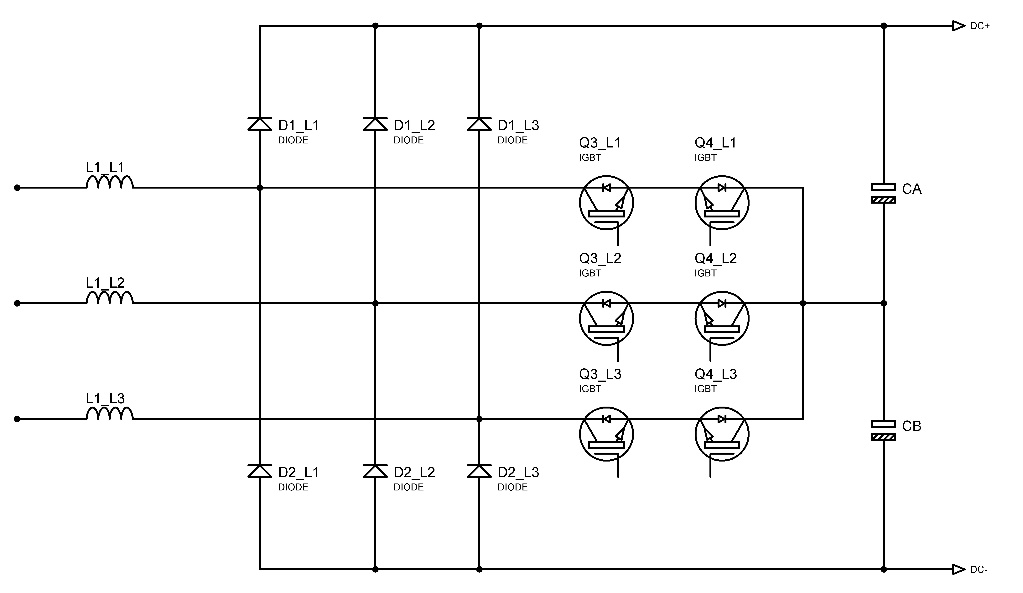
\includegraphics[width=0.92\textwidth]{gt-tipi/onceki_tez_6_2_viyana_pfc.jpeg}
  \caption{Vienna doğrultucu PFC devresi (ilk tasarım katmanı).}
  \label{fig:gt-viyana-pfc}
\end{figure}

Şekil~\ref{fig:gt-cok-sekonderli-bys}, tek primer ve çok sayıda sekonder sargı üzerinden her bataryaya ayrı doğrultucu--buck kolu sağlamaktadır. Her çıkışta diyot doğrultma, DA bağlantı kondansatörü, kontrollü anahtar, serbest dolaşım diyodu, endüktans ve çıkış kondansatörü bulunmaktadır. Batarya bazında şarj akımı ve gerilimi ayarlama hedefi sekonder kollarının fiziksel ayrışmasına dayanmaktadır.

\begin{figure}[htbp]
  \centering
  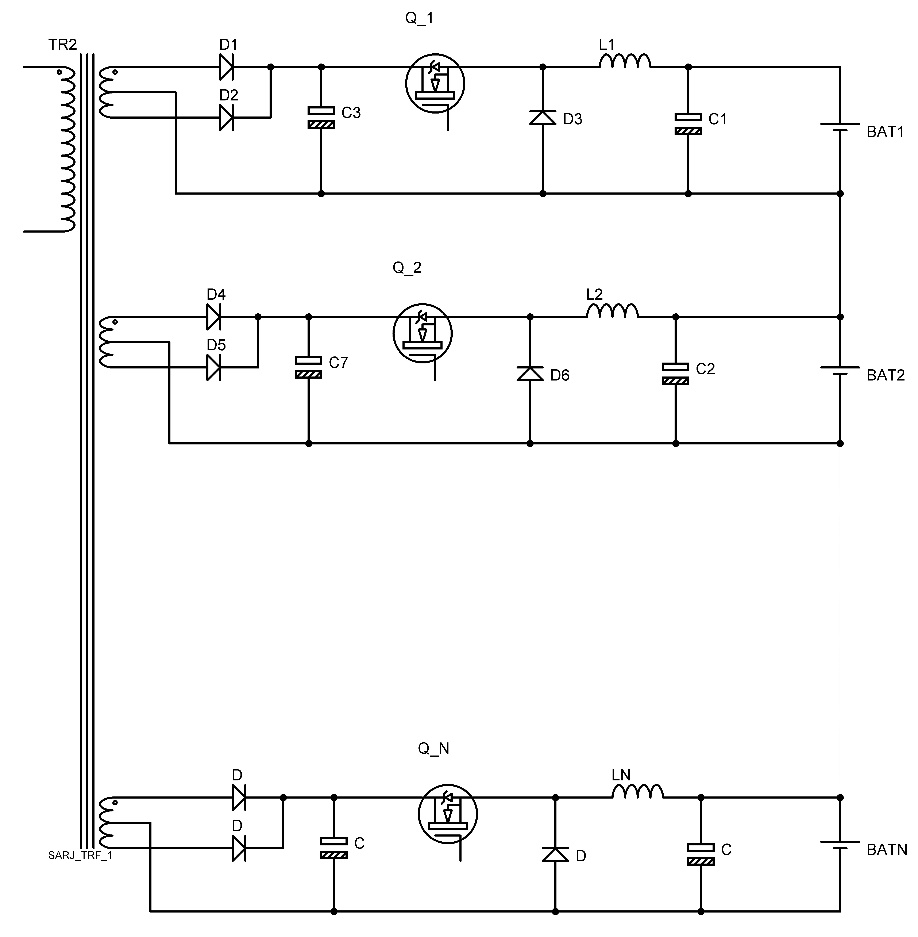
\includegraphics[width=0.67\textwidth]{gt-tipi/onceki_tez_6_3_cok_sekonderli_bys.jpeg}
  \caption{Tek primer ve çoklu sekonder sargılı transformatör içeren aktif BYS prensip devresi.}
  \label{fig:gt-cok-sekonderli-bys}
\end{figure}

Yaklaşımın ayırt edici bağlantısı Şekil~\ref{fig:gt-ana-topoloji} üzerinde görülmektedir. RL1, yarım köprü kolundaki $Q_1$--$Q_2$ anahtarları ile nötr kolundaki $Q_3$--$Q_4$ anahtarlarının ortak T-tipi çıkış düğümündeki işlevsel bağlantısını değiştirmektedir: bir konumda tam T-tipi evirici ve LCL filtre, diğer konumda iki seviyeli yüksek frekans katı ile ayrı PFC yolu oluşmaktadır.

\begin{figure}[htbp]
  \centering
  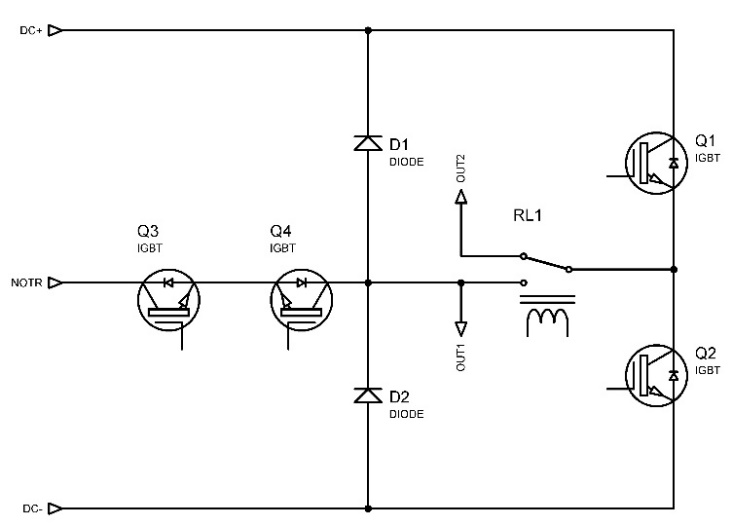
\includegraphics[width=0.82\textwidth]{gt-tipi/onceki_tez_6_4_gt_tipi_ana_topoloji.jpeg}
  \caption{GT-tipi ana topoloji ve RL1 fonksiyon anahtarı.}
  \label{fig:gt-ana-topoloji}
\end{figure}

RL1 ve RL2'nin evirici konumundaki bağlantısı Şekil~\ref{fig:gt-evirici-lcl} üzerinde gösterilmiştir. $Q_1$--$Q_4$ grubu bölünmüş DA bara ile faz çıkışı arasında üç seviyeli T-tipi kolu oluşturmakta; $L_1$--$C$--$L_2$ ağı şebeke akımını filtrelemektedir. Görsel, deşarj yönündeki temel güç yolunu açıklamaktadır; şebekeye deşarjın \SI{100}{\kilo\watt} prototip için gerçekleştirildiği anlamına gelmemektedir.

\begin{figure}[htbp]
  \centering
  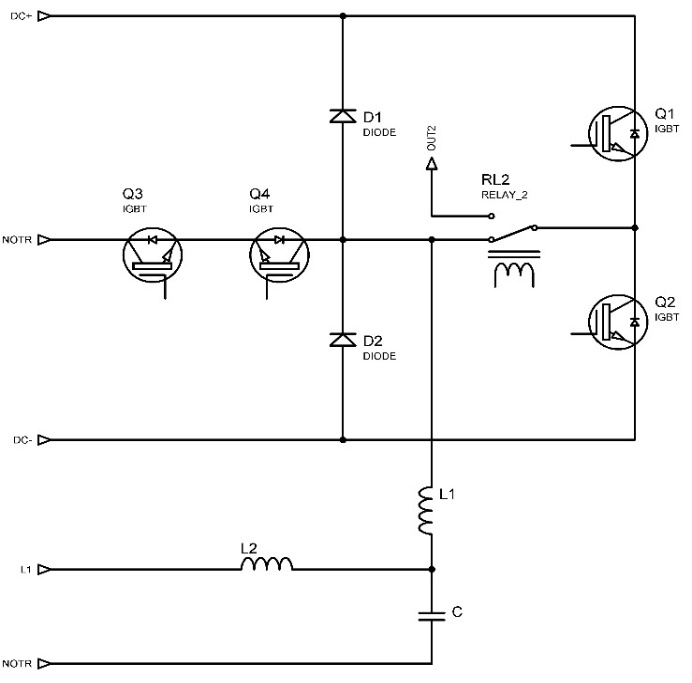
\includegraphics[width=0.76\textwidth]{gt-tipi/onceki_tez_6_5_evirici_lcl_modu.jpeg}
  \caption{GT-tipi topolojinin evirici çalışma modu ve LCL filtre bağlantısı.}
  \label{fig:gt-evirici-lcl}
\end{figure}

Şekil~\ref{fig:gt-iki-seviye-trafo}, üç fazın yarım köprü anahtarlarını üç adet çok sekonderli transformatörün primerleriyle ilişkilendirmektedir. Yalnız deşarjda kullanılan $Q_1$--$Q_2$ yarım köprülerinin şarj sırasında transformatör besleme katına dönüştürülmesi, yarı iletkenlerin atıl kalmasını önleyen birinci yeniden kullanım yoludur.

\begin{figure}[htbp]
  \centering
  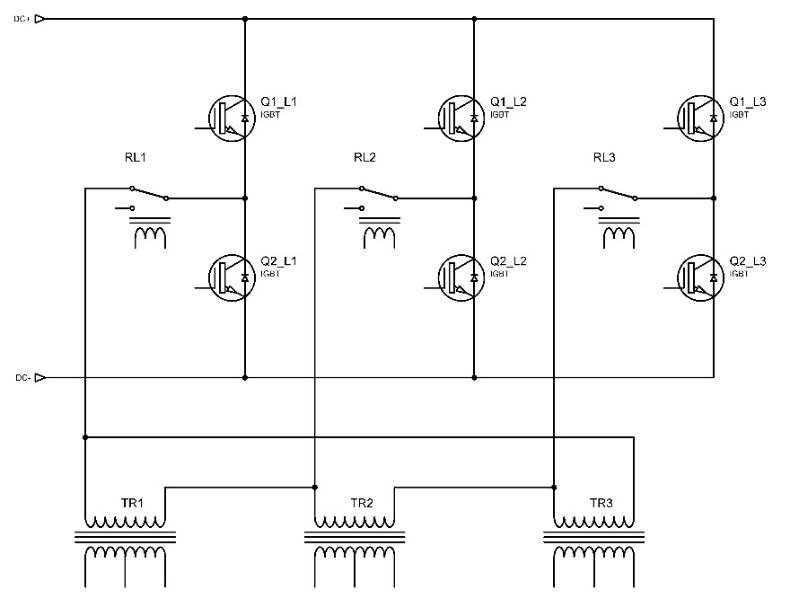
\includegraphics[width=0.88\textwidth]{gt-tipi/onceki_tez_6_6_iki_seviye_trafo_modu.jpeg}
  \caption{İki seviyeli evirici çıkışları ve çok sekonderli BYS transformatörleri.}
  \label{fig:gt-iki-seviye-trafo}
\end{figure}

İkinci yeniden kullanım yolu Şekil~\ref{fig:gt-pfc-modu} üzerinde verilmiştir: nötr IGBT çiftleri, doğrultma diyotları ve LCL elemanlarıyla üç fazlı Vienna PFC kollarına dönüştürülmektedir. Şekil~\ref{fig:gt-evirici-lcl}--\ref{fig:gt-pfc-modu} birlikte okunduğunda GT-tipi adının yalnız yeni bir devre çiziminden değil, aynı anahtar gruplarının enerji yönüne göre farklı görevlerde kullanılmasından kaynaklandığı görülmektedir.

\begin{figure}[htbp]
  \centering
  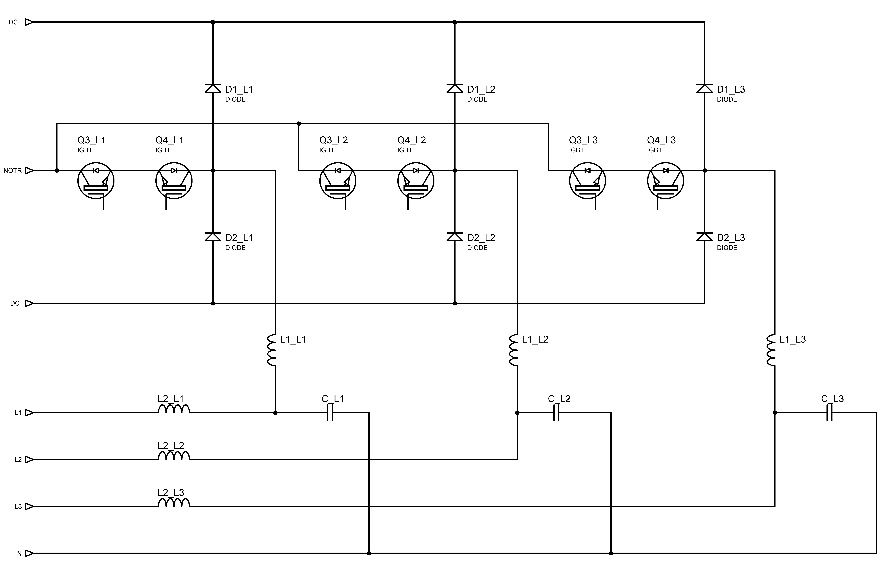
\includegraphics[width=0.94\textwidth]{gt-tipi/onceki_tez_6_7_pfc_modu.jpeg}
  \caption{Nötr IGBT gruplarıyla oluşturulan üç fazlı PFC bölümü.}
  \label{fig:gt-pfc-modu}
\end{figure}

\subsection{100 kW Hedefli Proje Mimarisi}

Şekil~\ref{fig:gt-basvuru-guc-kati}, proje başvuru formundaki değiştirilmiş T-tipi güç katını kaynağındaki işaretlerle korumaktadır. Şebeke tarafındaki transformatör, EMI filtresi ve LCL filtre sonrasında altı IGBT'li üç seviyeli PFC katı bulunmaktadır. Bölünmüş DA bara, diyot köprüleri ve altı SiC MOSFET'li yüksek frekanslı köprü, fazlar arasına bağlı transformatör gruplarını besleyecek biçimde gösterilmiştir. ``MOD'' işareti şarj ile deşarj yönündeki anahtarlama düzenini seçen üst seviye komutu temsil etmektedir. Şema kavramsal bağlantıyı gösterir; anahtar gerilim/akım değerleri, sürücü devreleri, ölü zamanlar, filtre elemanları ve koruma eşikleri verilmediğinden imalat şeması değildir.

\begin{figure}[htbp]
  \centering
  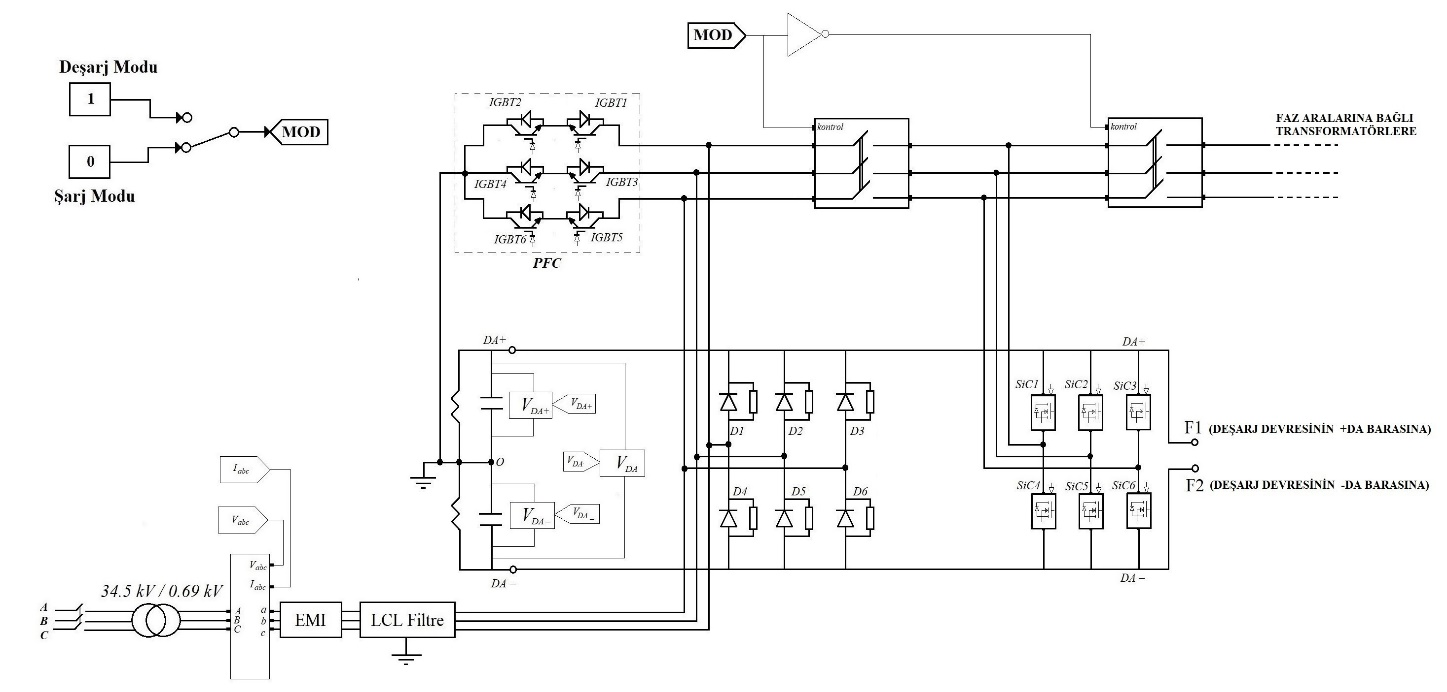
\includegraphics[width=0.98\textwidth]{gt-tipi/basvuru-degistirilmis-t-tipi-guc-kati.jpg}
  \caption{Proje başvuru kaynağındaki değiştirilmiş T-tipi, PFC özellikli güç katı ve fazlar arası transformatör çıkışları \citep{Arifoglu2023Basvuru}.}
  \label{fig:gt-basvuru-guc-kati}
\end{figure}

Sistem gücünün fazlar arası üç alt yapıya dengeli dağıtıldığı ideal durumda toplam güç referansı
\begin{equation}
  P_{\mathrm{GT}}^{\star}=P_{AB}^{\star}+P_{BC}^{\star}+P_{CA}^{\star},
  \qquad
  P_{AB}^{\star}\simeq P_{BC}^{\star}\simeq P_{CA}^{\star}\simeq
  \frac{P_{\mathrm{GT}}^{\star}}{3}
  \label{eq:gt-guc-paylasimi}
\end{equation}
biçiminde yazılabilir. Eşitlik~\eqref{eq:gt-guc-paylasimi} içinde $P_{\mathrm{GT}}^{\star}$ toplam hedef gücü; $P_{AB}^{\star}$, $P_{BC}^{\star}$ ve $P_{CA}^{\star}$ ilgili faz çifti konteynerlerinin güç referanslarını gösterir. \SI{100}{\kilo\watt} hedef için ideal dengeli pay yaklaşık \SI{33.3}{\kilo\watt} değerindedir; bölüşüm bir ölçüm sonucu değil, faz akımlarını dengeli tutmak için kullanılacak başlangıç tasarım koşuludur.

Şekil~\ref{fig:gt-basvuru-sarj-desarj}, AB konteyneri içinde çoğaltılan şarj/deşarj alt birimlerini, çok sekonderli yalıtım transformatörünü, batarya başına DA/DA kolunu ve seri deşarj yolunu birlikte göstermektedir; aynı yapı BC ve CA faz çiftleri için yinelenmektedir. Kaynak çizimde her konteynerde dokuz alt birim ve her alt birimde kırk sekonder çıkış üzerinden yirmi bataryaya ait iki kutuplu bağlantı gösterilmektedir. Sayıların nihai donanım yerleşimi sayılabilmesi için transformatör imalat dosyası, batarya konfigürasyonu ve kablolama listesi gereklidir.

\begin{figure}[htbp]
  \centering
  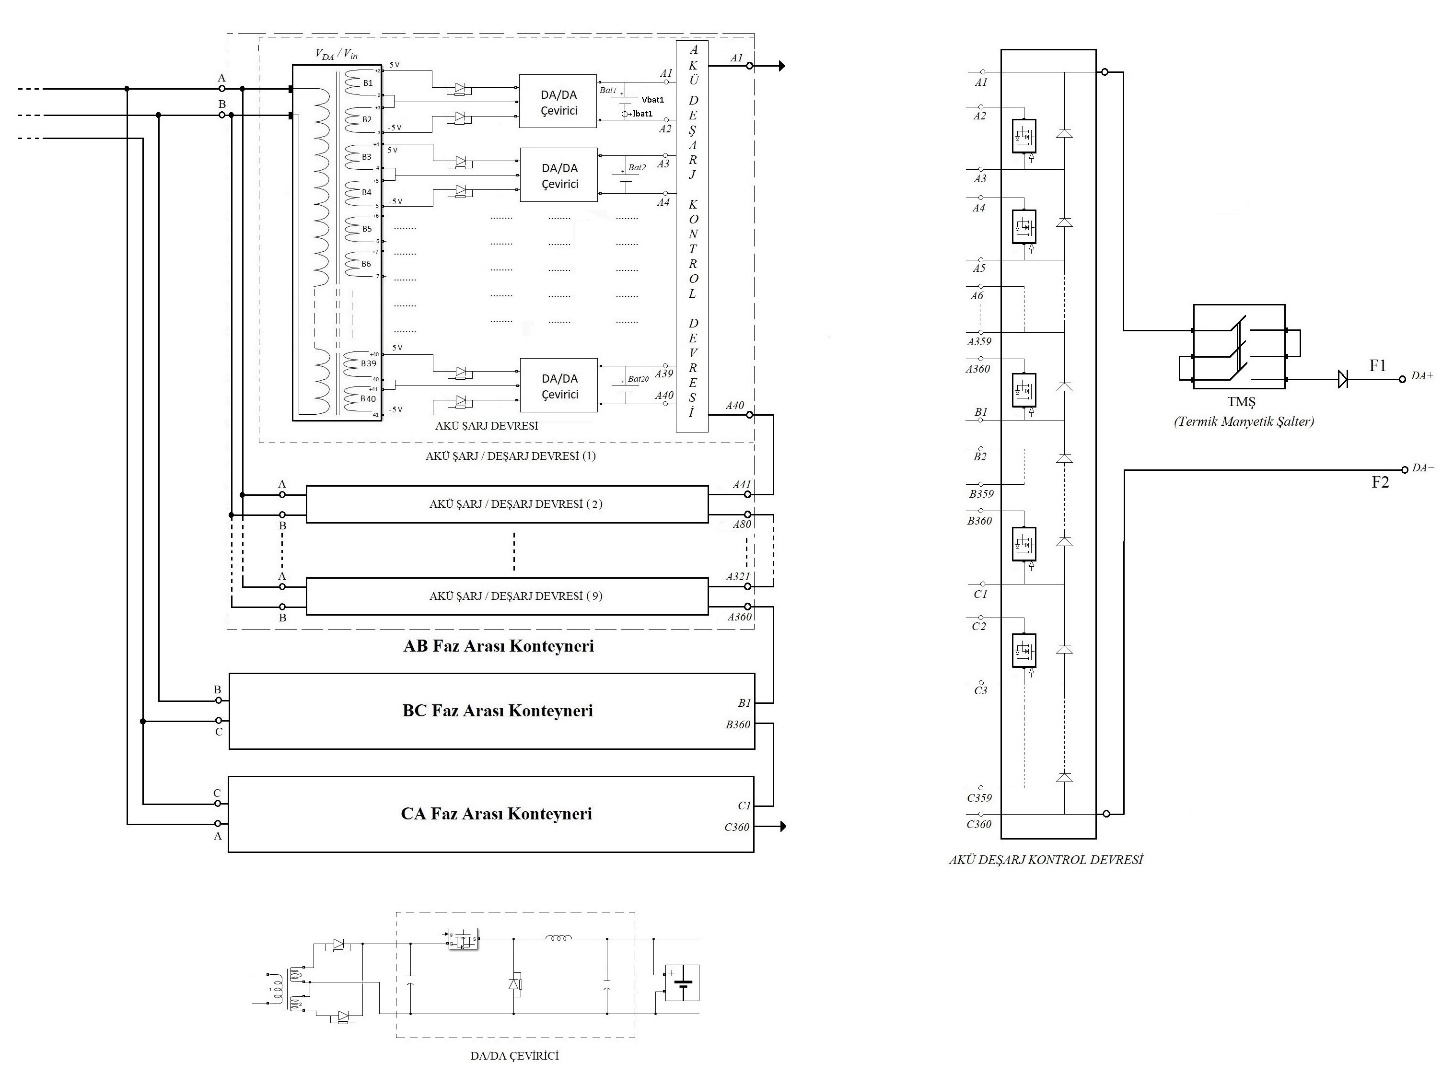
\includegraphics[width=0.96\textwidth]{gt-tipi/basvuru-sarj-desarj-konteyner-mimarisi.jpg}
  \caption{Proje başvuru kaynağındaki AB--BC--CA konteynerleri, izole şarj kolları ve seçilebilir seri deşarj yolu \citep{Arifoglu2023Basvuru}.}
  \label{fig:gt-basvuru-sarj-desarj}
\end{figure}

Batarya dizisindeki $N_b$ birimden hangilerinin seri deşarj yoluna alındığı $s_k\in\{0,1\}$ seçim değişkeniyle gösterildiğinde dizi geriliminin ideal bağıntısı
\begin{equation}
  v_{\mathrm{str}}(t)=\sum_{k=1}^{N_b}s_k(t)v_{b,k}(t)
  -\sum_{k=1}^{N_b}\bigl[1-s_k(t)\bigr]v_{D,k}(t)
  \label{eq:gt-dizi-gerilimi}
\end{equation}
olur. Eşitlik~\eqref{eq:gt-dizi-gerilimi} içinde $v_{\mathrm{str}}$ seri dizinin uç gerilimini, $v_{b,k}$ $k$ numaralı bataryanın uç gerilimini ve $v_{D,k}$ bypass yolundaki diyotun ileri yön gerilim düşümünü belirtmektedir; $s_k=1$ bataryanın seri yola alındığını, $s_k=0$ bypass edildiğini ifade eder. Gerçek devrede MOSFET iletim düşümü, kablo/bağlantı direnci ve anahtarlama geçişleri de eklenmelidir. Bağıntı, bypass edilen birim sayısı arttıkça DA bara gerilimi ile diyot kaybının birlikte değişeceğini açıklar.

Her bataryanın ayrı izole buck kolundan şarj edilmesi, seri deşarj bağlantısından farklı bir enerji yolu oluşturur. Şarj durumunda batarya akımları bağımsız ayarlanabilirken deşarj durumunda etkin birimlerden aynı dizi akımı geçer. İşlev ayrımı, ``batarya bazında dengeleme'' hedefinin şarj ve deşarj için aynı fiziksel mekanizmaya dayanmadığını gösterir: şarjda bağımsız akım/gerilim düzenleme, deşarjda birim seçimi ve bypass kullanılmaktadır.

\begin{figure}[htbp]
  \centering
  \begin{tikzpicture}[
    font=\small,
    block/.style={draw,rounded corners,align=center,minimum width=26mm,minimum height=12mm,fill=blue!5},
    batt/.style={draw,rounded corners,align=center,minimum width=26mm,minimum height=12mm,fill=green!8},
    ctrl/.style={draw,rounded corners,align=center,minimum width=29mm,minimum height=12mm,fill=orange!10},
    flow/.style={-{Latex[length=2.2mm]},thick},
    signal/.style={-{Latex[length=2mm]},dashed}
  ]
    \node[block] (grid) {\SI{690}{\volt} AA\\EMI + LCL};
    \node[block,right=9mm of grid] (pfc) {Değiştirilmiş\\T-tipi PFC};
    \node[block,right=9mm of pfc] (dc) {Bölünmüş\\DA bara};
    \node[block,right=9mm of dc] (sic) {SiC köprü\\\SI{30}{\kilo\hertz}};
    \node[block,below=12mm of sic] (tr) {AB--BC--CA\\yalıtım trafoları};
    \node[batt,left=9mm of tr] (buck) {Batarya başına\\izole buck};
    \node[batt,left=9mm of buck] (battery) {Batarya dizileri\\ve yedek birimler};
    \node[batt,below=12mm of battery] (load) {Seçilebilir seri yol\\ve kademeli DA yük};
    \node[ctrl,below=12mm of dc] (ems) {Üst seviye kip ve\\güç paylaşım denetimi};

    \draw[flow] (grid) -- node[above,font=\scriptsize]{şarj} (pfc);
    \draw[flow] (pfc) -- (dc);
    \draw[flow] (dc) -- (sic);
    \draw[flow] (sic) -- (tr);
    \draw[flow] (tr) -- (buck);
    \draw[flow] (buck) -- (battery);
    \draw[flow] (battery) -- node[left,font=\scriptsize]{deşarj} (load);
    \draw[signal] (ems) -- (pfc);
    \draw[signal] (ems) -- (sic);
    \draw[signal] (ems) -- (buck);
    \draw[signal] (ems) -- (battery);
  \end{tikzpicture}
  \caption{Kaynak şemalardan sentezlenen GT-tipi enerji ve denetim katmanları; oklar şarj ve kademeli yüke deşarj yönlerini göstermektedir.}
  \label{fig:gt-sentez-mimarisi}
\end{figure}

Şekil~\ref{fig:gt-sentez-mimarisi}, kaynak çizimlerde farklı sayfalara dağılan güç ve denetim katmanlarını tek bir işlevsel akışta birleştirmektedir. PFC katı şebeke akımı ile DA bara gerilimini, SiC köprü ve transformatör katı yalıtılmış enerji aktarımını, batarya başına buck kolları şarj akım/gerilimlerini, seri seçim ağı ise deşarj gerilimini belirler. Aynı anda bütün katların hızlı anahtarlanması gerekmez; batarya seçimi ve kip geçişleri, güç dönüştürücü PWM'inden daha yavaş bir üst seviye durum makinesiyle yönetilmelidir.

\section{Şarj Yönündeki Benzetim Kayıtları}
\label{sec:gt-benzetim}

GT-tipi topolojinin şarj yönündeki işlevsel bütünlüğü; Vienna PFC, iki seviyeli transformatör besleme katı ve batarya şarj kolunu aynı Simulink modeli içinde çalıştıran bir benzetimle gösterilmiştir. Şekil~\ref{fig:gt-simulink-modeli}--\ref{fig:gt-batarya-soc} yalnız sonuç grafikleri değildir; şebekeden bataryaya uzanan PFC $\rightarrow$ DA bara $\rightarrow$ transformatör primeri $\rightarrow$ sekonder $\rightarrow$ buck/batarya zincirinin her aşamasını belgelemektedir. Kaynak model dosyası ve ham zaman serileri mevcut olmadığı için kayıtlar bağımsız olarak yeniden hesaplanamamaktadır; kanıt statüleri nitel gösterim düzeyiyle sınırlandırılmıştır.

Şekil~\ref{fig:gt-simulink-modeli}; PFC denetimi, DA bara, üç fazlı dönüştürücü, çok sekonderli transformatörler ve batarya alt sistemlerinin aynı modelde kurulduğunu göstermektedir. Ekran görüntüsü blok adlarını ayrıntılı incelemek için yeterli çözünürlükte değildir; model hiyerarşisinin ve sonuç zincirinin varlığını belgelemek amacıyla verilmiştir.

\begin{figure}[htbp]
  \centering
  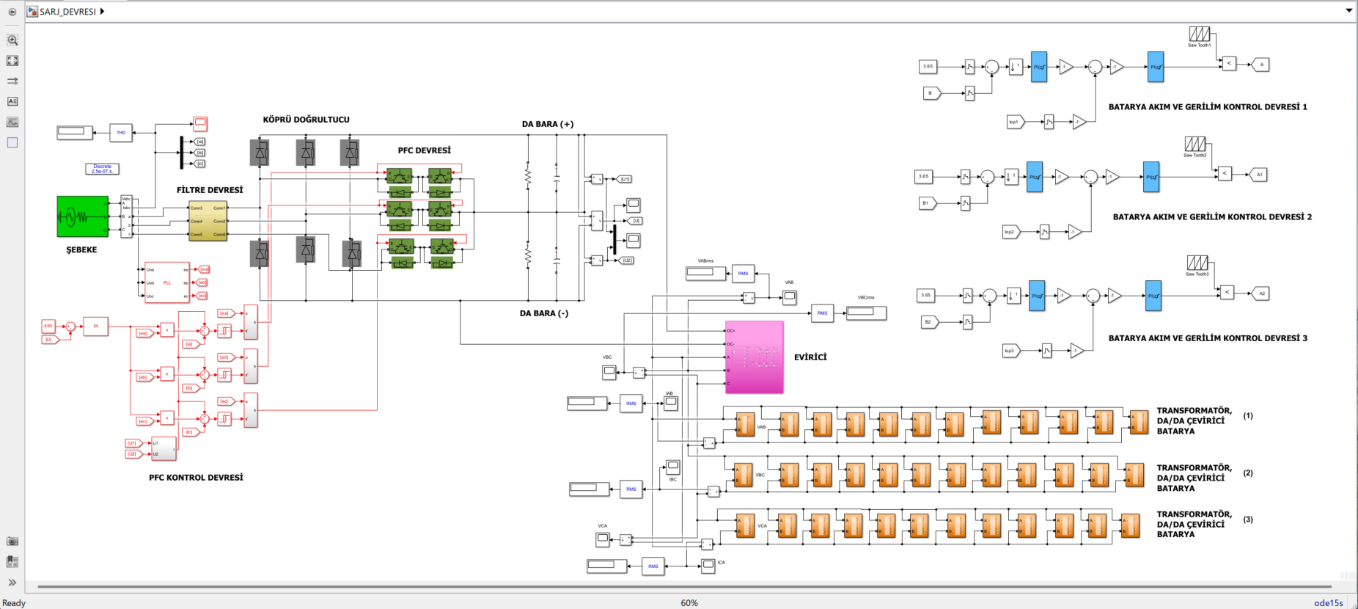
\includegraphics[width=0.98\textwidth]{gt-tipi/onceki_tez_6_8_simulink_modeli.png}
  \caption{Şarj yönündeki Vienna PFC, iki seviyeli evirici ve transformatör tabanlı BYS Simulink modeli.}
  \label{fig:gt-simulink-modeli}
\end{figure}

Şekil~\ref{fig:gt-pfc-akimlari}, PFC sonrasında üç faz akımının dengeli ve yaklaşık sinüzoidal biçimde oluştuğunu göstermektedir. Eksen birimleri, başlangıç koşulu, analiz penceresi, THD hesabı ve model parametreleri grafikten tek başına doğrulanamadığından görsel, PFC işlevinin çalıştığına ilişkin nitel kanıt olarak kullanılmıştır.

\begin{figure}[htbp]
  \centering
  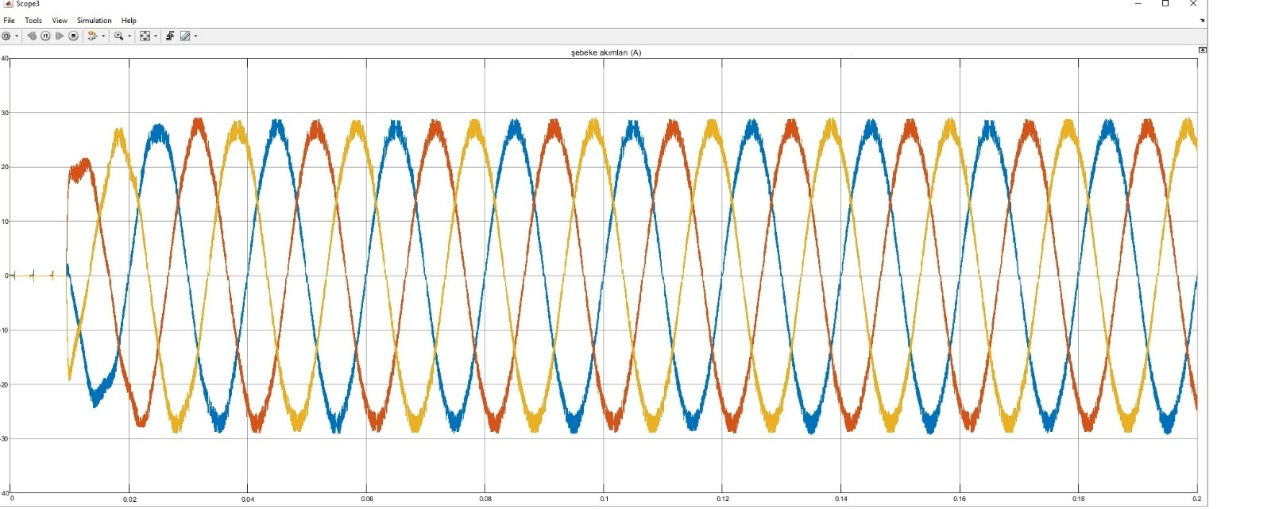
\includegraphics[width=0.96\textwidth]{gt-tipi/onceki_tez_6_9_pfc_sebeke_akimlari.jpeg}
  \caption{Vienna PFC sonrasındaki üç faz şebeke akımları.}
  \label{fig:gt-pfc-akimlari}
\end{figure}

Şekil~\ref{fig:gt-da-bara}, DA bara gerilimlerinin başlangıç geçicisinden sonra birbirine yakın bir çalışma bandına yerleştiğini göstermektedir. Referansın toplam bara mı, yarım bara mı olduğu ve düşey eksenin kesin değeri ham model olmadan kilitlenemediğinden grafik yalnız regülasyon davranışını nitel olarak destekler.

\begin{figure}[htbp]
  \centering
  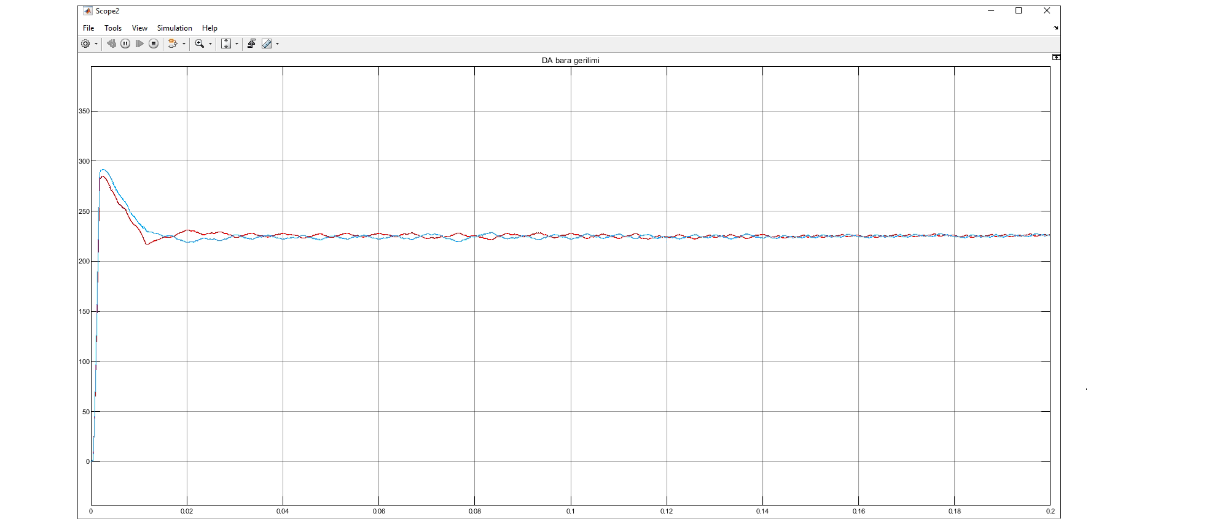
\includegraphics[width=0.96\textwidth]{gt-tipi/onceki_tez_6_10_da_bara_gerilimleri.png}
  \caption{DA bara gerilimlerinin zamanla değişimi.}
  \label{fig:gt-da-bara}
\end{figure}

İki seviyeli yüksek frekans katının transformatör primerine uyguladığı gerilim Şekil~\ref{fig:gt-primer-gerilim}, primer akımı Şekil~\ref{fig:gt-primer-akim} üzerindedir. Primer geriliminin pozitif, sıfır ve negatif seviyeler arasında değişmesi, görev oranı üzerinden transformatöre aktarılan gücün ayarlanabildiğini gösterir. Primer akımı aynı anahtarlama dizisine yanıt vermekte; kenarlardaki eğimler eşdeğer endüktans ve manyetik devre dinamiğinin etkisini göstermektedir. Sayısal kayıp veya transformatör verimi, sarım ve manyetik parametreler bulunmadan çıkarılmamıştır.

\begin{figure}[htbp]
  \centering
  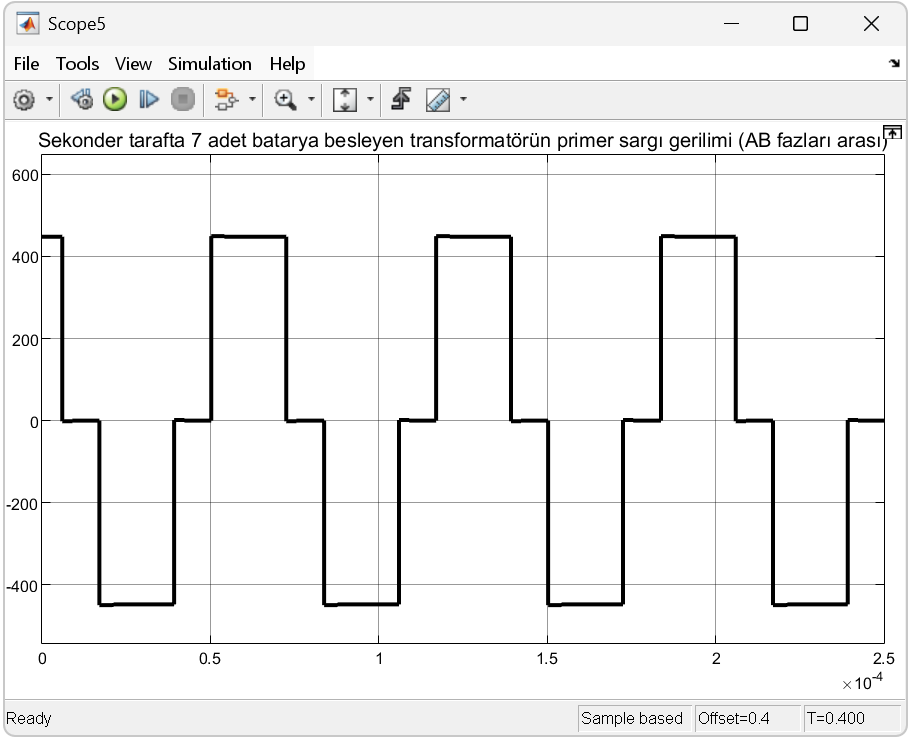
\includegraphics[width=0.76\textwidth]{gt-tipi/onceki_tez_6_11_primer_gerilim.png}
  \caption{BYS transformatörü primer sargı gerilimi.}
  \label{fig:gt-primer-gerilim}
\end{figure}

\begin{figure}[htbp]
  \centering
  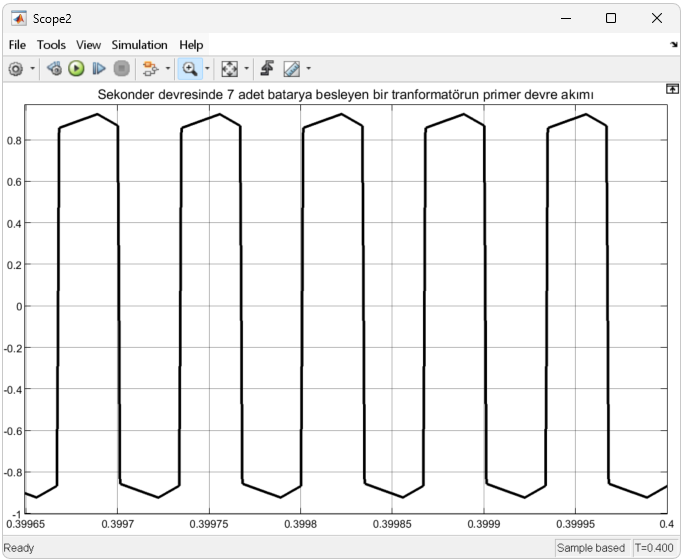
\includegraphics[width=0.76\textwidth]{gt-tipi/onceki_tez_6_12_primer_akim.png}
  \caption{BYS transformatörü primer akımı.}
  \label{fig:gt-primer-akim}
\end{figure}

Şekil~\ref{fig:gt-sekonder-gerilim} ve Şekil~\ref{fig:gt-sekonder-akim}, bir bataryayı besleyen sekonder sargının doğrultma öncesi gerilim ve akımını göstermektedir. Gerilim işaret değiştiren darbeli yapıya sahipken akımın pozitif enerji aktarım aralıklarında belirginleşmesi, sekonder doğrultucu ve buck girişinin primer anahtarlamasıyla eşzamanlı çalıştığını gösterir. Dönüş oranı, kaçak endüktans ve doğrultucu düşümleri bilinmediğinden primer--sekonder genlikleri üzerinden kesin verim hesabı yapılmamıştır.

\begin{figure}[htbp]
  \centering
  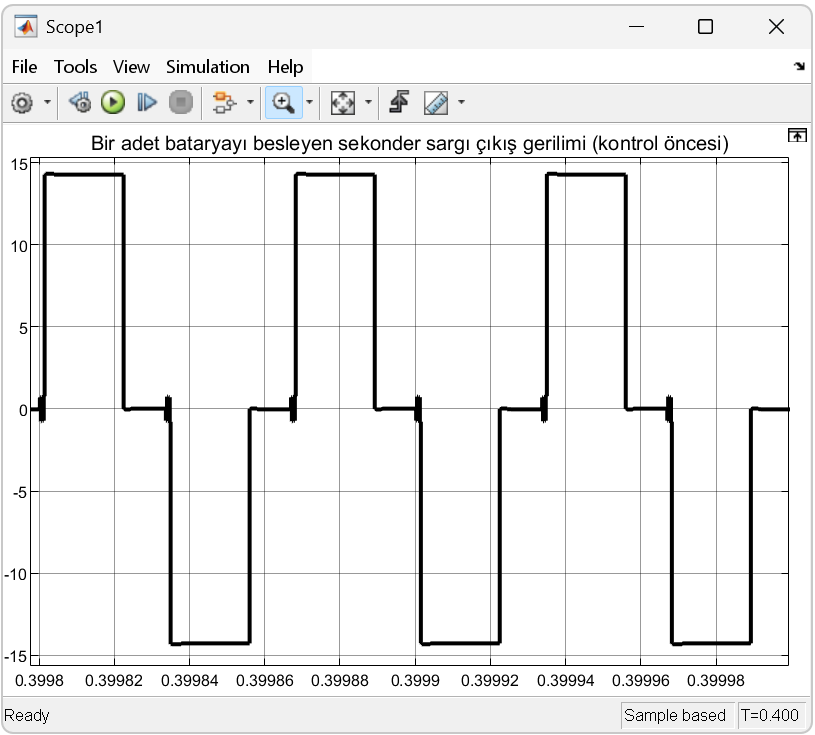
\includegraphics[width=0.76\textwidth]{gt-tipi/onceki_tez_6_13_sekonder_gerilim.png}
  \caption{BYS transformatörü sekonder sargı gerilimi.}
  \label{fig:gt-sekonder-gerilim}
\end{figure}

\begin{figure}[htbp]
  \centering
  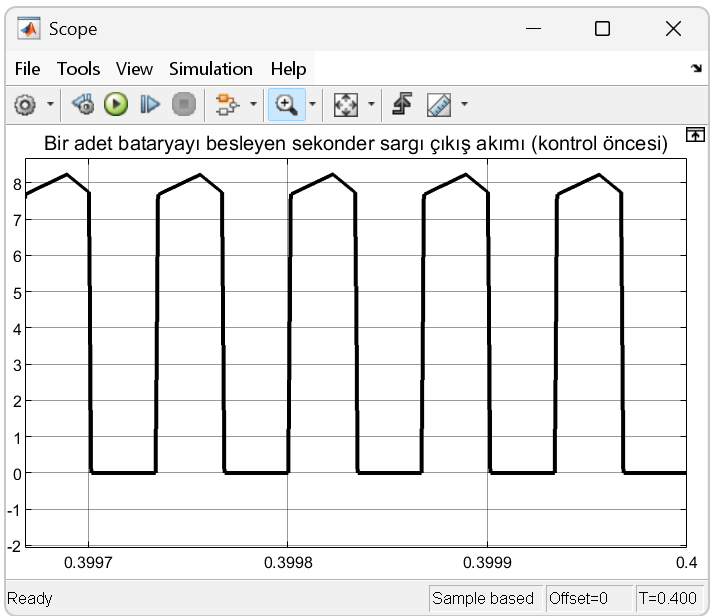
\includegraphics[width=0.76\textwidth]{gt-tipi/onceki_tez_6_14_sekonder_akim.png}
  \caption{BYS transformatörü sekonder sargı akımı.}
  \label{fig:gt-sekonder-akim}
\end{figure}

Enerji zincirinin batarya tarafındaki son kaydı Şekil~\ref{fig:gt-batarya-soc} üzerindedir; bir bataryanın şarj durumu (State of Charge, SoC), uç gerilimi ve akımı aynı zaman ekseninde verilmiştir. İşaret yönü ve ölçekler model değişken tanımlarına bağlı olduğundan değerler fiziksel deney sonucu olarak yorumlanmamıştır; kaydın görevi, PFC ve transformatör dalga biçimlerinin batarya durumuyla ilişkilendirildiğini göstermektir.

\begin{figure}[htbp]
  \centering
  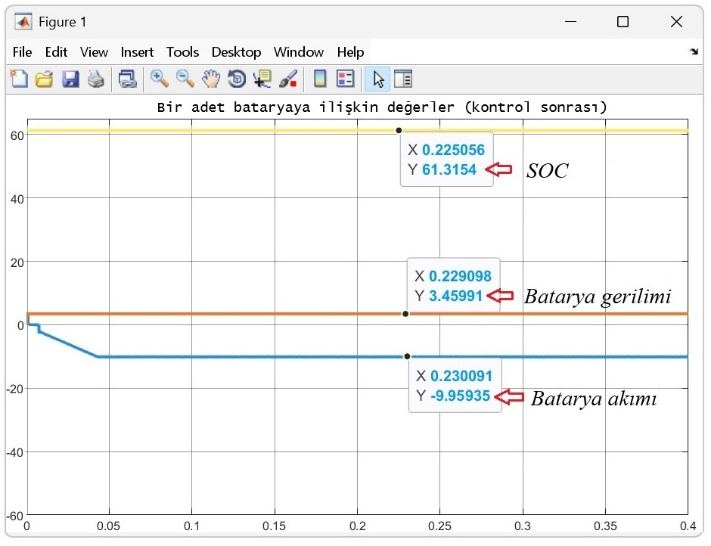
\includegraphics[width=0.80\textwidth]{gt-tipi/onceki_tez_6_15_batarya_soc.jpeg}
  \caption{Bir bataryaya ait SoC, uç gerilimi ve akım kayıtları.}
  \label{fig:gt-batarya-soc}
\end{figure}

Kayıtlar birlikte değerlendirildiğinde şarj yönündeki enerji aktarım zincirinin bütün alt basamakları temsil edilmektedir. Aynı kayıtlar; deşarj yönünde T-tipi evirici çalışmasını, RL1 geçişini, bypass/yedekleme davranışını, farklı güç seviyelerini veya deneysel performansı doğrulamamaktadır.

Şarj zinciri kayıtlarının yeniden üretilmesi için gereken kaynak model dosyası, çağrılan parametre dosyaları, çözücü ayarları, PFC ve DA bara referansları, anahtarlama frekansları ile transformatör ve batarya parametreleri tez kapsamında bulunmamaktadır. \SI{100}{\kilo\watt} katman için de güç kartı şeması, malzeme listesi (Bill of Materials, BOM), SiC, IGBT, MOSFET ve diyot parça kodları, çok sekonderli transformatörün sarım ve izolasyon bilgileri, batarya kimyası ve kapasitesi tanımlı değildir. Şekil~\ref{fig:gt-simulink-modeli}--\ref{fig:gt-batarya-soc} kayıtları ham zaman serisinden yeniden hesaplanamadığından THD, güç faktörü, verim ve SoC için sayısal sonuç verilmemekte; kayıtlar yalnız şarj zincirinin işlevsel bütünlüğüne ilişkin nitel gösterim olarak kullanılmaktadır. Sınırlılık açıktır: GT-tipi mimari için tezde yeniden üretilebilir benzetim kanıtı ve deney kanıtı yoktur; mimari, bir öneri ve gelecek çalışma konusu düzeyinde sunulmaktadır. Anahtarlamalı modelin kurulması ve ölçekli prototip deneyi, Bölüm~\ref{sec:gt-dogrulama} altındaki doğrulama matrisinin ilk adımları olarak gelecek çalışmaya bırakılmıştır.

\section{Şarj ve Deşarj Çalışma Modları}
\label{sec:gt-modlar}

GT-tipi yapının çalışması tek bir ``çift yönlü'' komutla açıklanamaz. Şebeke katı, yüksek frekans köprüsü, batarya buck kolları, seri seçim anahtarları, kontaktörler ve bypass yolları için izin verilen durumların birlikte tanımlanması gerekir. Tablo~\ref{tab:gt-calisma-modlari}, kaynak belgedeki işlevleri güvenli bir durum dizisine dönüştürmektedir.

\begin{table}[H]
  \centering
  \caption{GT-tipi mimarinin önerilen çalışma modları ve geçiş koşulları.}
  \label{tab:gt-calisma-modlari}
  \small
  \begin{tabularx}{\textwidth}{@{}p{0.18\textwidth}p{0.23\textwidth}X@{}}
    \toprule
    Mod & Etkin güç yolu & Temel koşul ve amaç \\
    \midrule
    Güvenli kapalı & Bütün PWM'ler ve ana kontaktörler kapalı & Enerjisiz başlatma, kilitli hata veya bakım durumu; artık gerilim denetlenir. \\
    Ön şarj / öz sınama & Sınırlı akımlı DA bara yolu ve ölçümler & İzolasyon, kontaktör geri bildirimi, sensör makullüğü ve DA bara gerilim yükselme hızı kontrol edilir. \\
    Şebekeden şarj & EMI--LCL--T-tipi PFC--DA bara--SiC köprü--trafo--buck--batarya & Şebeke akımı, DA bara, transformatör ve batarya sınırları birlikte korunur. \\
    CC şarj & Batarya başına buck akım düzenleme & Batarya üreticisinin akım ve sıcaklık sınırları içinde sabit akım uygulanır. \\
    CV şarj & Batarya başına buck gerilim düzenleme & Üst gerilim sınırında akım azalıncaya kadar sabit gerilim uygulanır. \\
    Kademeli yüke deşarj & Seçilen bataryalar--seri MOSFET yolu--DA yük & Şebekeye enerji verilmeden yük bankasına güç aktarılır; dizi gerilimi birim seçimiyle ayarlanır. \\
    Bypass / yedekleme & Zayıf birim devre dışı, bypass diyodu ve uygun yedek birim etkin & Gerilim, sıcaklık, SoC veya hata sınırını aşan birimin seri akım yolunu kesmeden ayrılması hedeflenir. \\
    Bakım/darbe modu & Yalnız uygun kimyadaki seçilmiş batarya ve buck kolu & Desülfasyon/hafıza etkisi işlemi genel EDS modu değildir; üretici sınırı, kimya ve deney protokolü doğrulanmadan etkinleştirilmez. \\
    \bottomrule
  \end{tabularx}
\end{table}

Batarya başına şarj referansı, CC--CV geçişini açıkça göstermek için
\begin{equation}
  i_{b,k}^{\star}=
  \begin{cases}
    I_{\mathrm{CC},k}, & v_{b,k}<V_{\mathrm{CV},k}\ \land\ T_{\min,k}<T_{b,k}<T_{\max,k},\\
    \operatorname{sat}\!\left[K_{v,k}\left(V_{\mathrm{CV},k}-v_{b,k}\right),0,I_{\mathrm{CC},k}\right],
      & v_{b,k}\geq V_{\mathrm{CV},k},\\
    0, & \text{koruma veya bypass koşulu}
  \end{cases}
  \label{eq:gt-cccv-referansi}
\end{equation}
biçiminde tanımlanabilir. Eşitlik~\eqref{eq:gt-cccv-referansi} içinde $i_{b,k}^{\star}$ $k$ numaralı bataryanın şarj akımı referansını, $I_{\mathrm{CC},k}$ sabit akım sınırını, $V_{\mathrm{CV},k}$ sabit gerilim eşiğini, $T_{b,k}$ ölçülen batarya sıcaklığını, $T_{\min,k}$ ve $T_{\max,k}$ izin verilen sıcaklık sınırlarını, $K_{v,k}$ gerilim düzenleyici kazancını ve $\operatorname{sat}[\cdot]$ doyum işlemini göstermektedir. Sayısal sınırlar batarya kimyası ve üretici veri sayfasından alınmadan atanmayacaktır.

Coulomb sayımına dayalı ayrık zamanlı şarj durumu güncellemesi
\begin{equation}
  \operatorname{SoC}_k[n+1]=\operatorname{sat}\!\left[
  \operatorname{SoC}_k[n]+\frac{\eta_{c,k}i_{b,k}[n]T_s}{Q_{n,k}},\,0,\,1\right]
  \label{eq:gt-soc-guncelleme}
\end{equation}
olarak yazılmıştır \citep{Plett2015}. Eşitlik~\eqref{eq:gt-soc-guncelleme} içinde $\operatorname{SoC}_k[n]$ $n$ örnekleme anındaki şarj durumunu, $\eta_{c,k}$ Coulomb verimini, $i_{b,k}[n]$ işaretli batarya akımını, $T_s$ BYS örnekleme süresini ve $Q_{n,k}$ güncel kullanılabilir kapasiteyi belirtmektedir; akım işareti şarj yönünde pozitif seçilmiştir. Akım sensörü ofseti ve kapasite yaşlanması nedeniyle yalnız Coulomb sayımı uzun süreli kullanımda sürüklenebilir; başlangıç düzeltmesi ve periyodik kestirim güncellemesi ayrıca tanımlanmalıdır.

Şekil~\ref{fig:gt-basvuru-tetikleme}, başvuru kaynağında DA bara/PFC denetimi ile SiC köprü darbe düzenini aynı görselde vermektedir. Üst kısımda \SI{1000}{\volt} DA bara referansı, PLL tabanlı faz bilgisi ve IGBT kapı komutları; alt kısımda \SI{30}{\kilo\hertz} temel dizilim ve görev oranı $d$ ile kısaltılan SiC darbeleri gösterilmiştir. Kaynak çizim; denetleyici katsayılarını, örnekleme sürelerini, ölü zamanı, doyumları ve koruma önceliğini eksiksiz vermediğinden gerçek zamanlı kodun yerine kullanılamaz.

\begin{figure}[H]
  \centering
  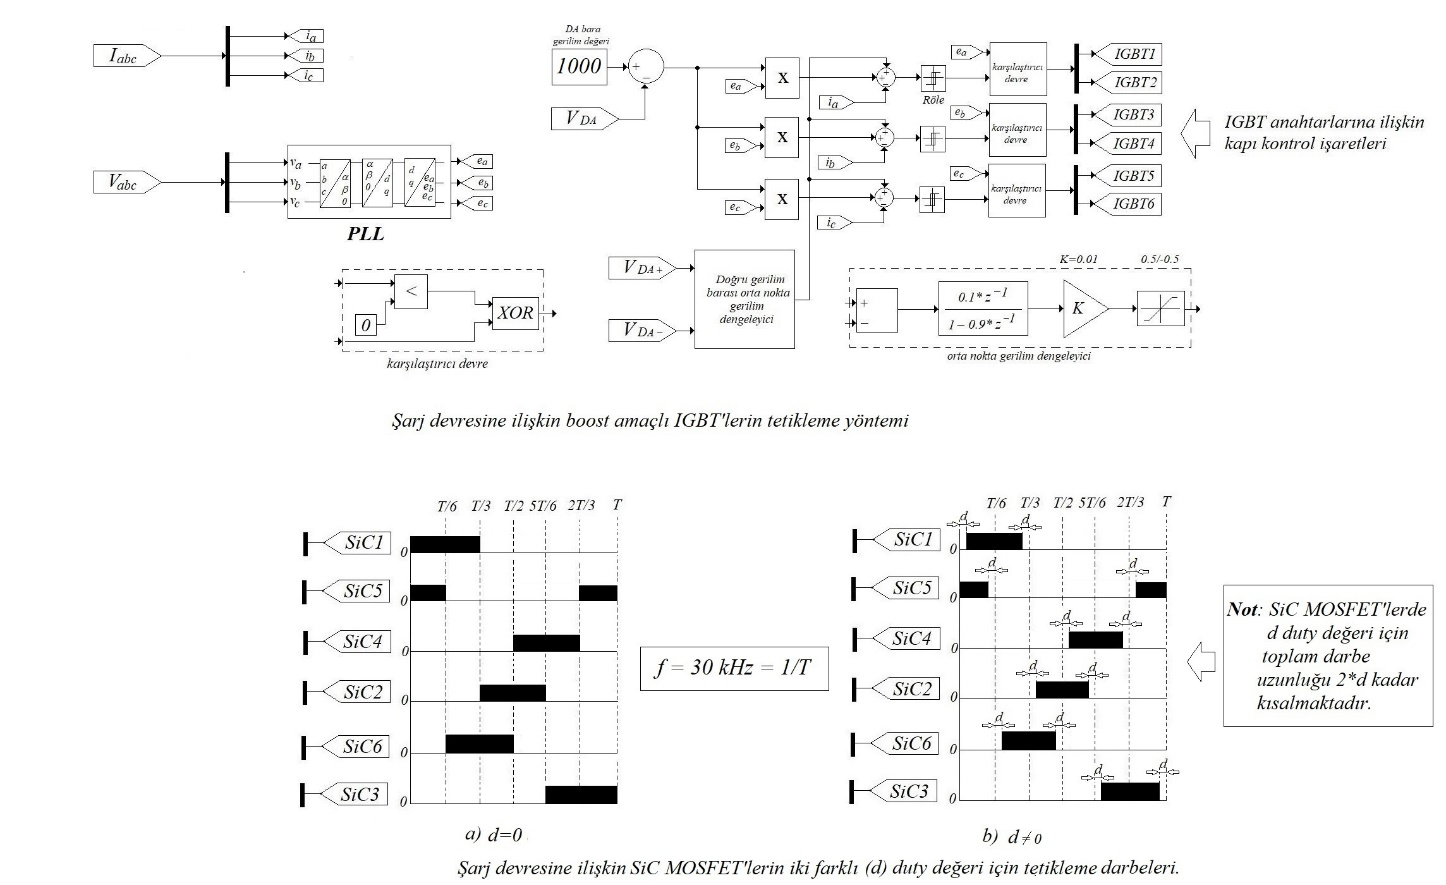
\includegraphics[width=0.96\textwidth]{gt-tipi/basvuru-igbt-sic-tetikleme.jpg}
  \caption{Proje başvuru kaynağındaki IGBT PFC denetimi ve iki farklı görev oranı için SiC MOSFET tetikleme düzeni \citep{Arifoglu2023Basvuru}.}
  \label{fig:gt-basvuru-tetikleme}
\end{figure}

Şekil~\ref{fig:gt-basvuru-tetikleme} içindeki IGBT eşlemeleri, PLL işaretleri, karşılaştırıcı mantığı, nötr nokta dengelemesi, SiC sırası, görev oranı tanımı, ölü zaman ve PWM güncelleme anı gerçek kontrol kodu ya da kesin bir Simulink modeliyle doğrulanmamıştır; tetikleme düzeni tezde nitel bir denetim mimarisi olarak sunulmaktadır. Başvuru metnindeki \SI{3}{\kilo\hertz} desülfasyon ifadesinin buck çıkış referans darbesine mi yoksa anahtarlama frekansına mı ait olduğu kaynak belgeden belirlenememektedir; ifade sayısal tasarım değeri olarak kullanılmamıştır. Desülfasyon, yalnız uygun kurşun-asit ya da NiCd kimyası ve üretici sınırları için geçerli bir bakım kipi olarak ele alınmakta, lityum iyon bataryalara genellenmemektedir. Gömülü yazılımın gerçeklenmesi ve tetikleme mantığının donanım üzerinde doğrulanması gelecek çalışma kapsamındadır.

\section{Mod Geçişleri ve Güvenlik Kısıtları}
\label{sec:gt-gecis-guvenlik}

Yeniden yapılandırma sırasında iki farklı gerilimdeki batarya veya bara düğümünün doğrudan birleştirilmesi, sınırlanmamış dengeleme akımına ve arka neden olabilir. Seri seçim ağı için \emph{önce kes--sonra bağla} ilkesi, sıfıra yakın dizi akımı ve düğüm gerilimi eşleşmesi birlikte aranmalıdır. Önerilen izin koşulu
\begin{equation}
  \gamma_{k\rightarrow j}=1
  \iff
  |i_{\mathrm{str}}|\leq I_{\mathrm{tr}}
  \ \land\
  |v_{\mathrm{node},k}-v_{\mathrm{node},j}|\leq \Delta V_{\mathrm{tr}}
  \ \land\
  h_k=h_j=1
  \label{eq:gt-gecis-izni}
\end{equation}
şeklinde ifade edilmiştir. Eşitlik~\eqref{eq:gt-gecis-izni} içinde $\gamma_{k\rightarrow j}$ $k$ durumundan $j$ durumuna geçiş iznini, $i_{\mathrm{str}}$ seri dizi akımını, $I_{\mathrm{tr}}$ geçiş için izin verilen akım eşiğini, $v_{\mathrm{node},k}$ ve $v_{\mathrm{node},j}$ bağlanacak düğümlerin gerilimlerini, $\Delta V_{\mathrm{tr}}$ izin verilen gerilim farkını ve $h_k,h_j$ ilgili kontaktör/anahtar geri bildirimlerinin sağlıklı olduğunu gösterir. Sayısal eşikler yarı iletken güvenli çalışma alanı, bağlantı endüktansı, ön şarj direnci ve ölçüm belirsizliğiyle belirlenmelidir.

\begin{figure}[htbp]
  \centering
  \begin{tikzpicture}[
    scale=0.95,
    transform shape,
    node distance=9mm and 13mm,
    state/.style={draw,rounded corners,align=center,minimum width=27mm,minimum height=10mm,fill=blue!5,font=\small},
    safe/.style={state,fill=green!10},
    fault/.style={state,fill=red!8},
    arr/.style={-{Latex[length=2mm]},thick},
    guard/.style={font=\scriptsize,align=center}
  ]
    \node[safe] (off) {Güvenli kapalı};
    \node[state,right=of off] (pre) {Ön şarj ve\\öz sınama};
    \node[state,right=of pre] (ready) {Hazır};
    \node[state,below left=of ready] (charge) {Şarj\\PFC + CC/CV};
    \node[state,below right=of ready] (dis) {Deşarj\\kademeli yük};
    \node[state,below=of ready] (reconf) {Bypass /\\yeniden yapılandırma};
    \node[fault,below=19mm of reconf] (fault) {Kilitli hata};

    \draw[arr] (off) -- node[above,guard]{başlat} (pre);
    \draw[arr] (pre) -- node[above,guard]{ölçüm ve\\geri bildirim uygun} (ready);
    \draw[arr] (ready) -- node[left,guard]{şarj izni} (charge);
    \draw[arr] (ready) -- node[right,guard]{yük hazır} (dis);
    \draw[arr] (charge) -- node[above,guard]{akım sıfıra yakın} (reconf);
    \draw[arr] (dis) -- node[above,guard]{akım sıfıra yakın} (reconf);
    \draw[arr] (reconf) -- node[right,guard]{gerilim eşleşti} (ready);
    \draw[arr] (pre) |- (fault);
    \draw[arr] (charge) -- (fault);
    \draw[arr] (dis) -- (fault);
    \draw[arr] (reconf) -- (fault);
    \draw[arr] (fault) -| node[below,guard]{enerji kesme ve\\yetkili sıfırlama} (off);
  \end{tikzpicture}
  \caption{GT-tipi güvenli durum geçişleri.}
  \label{fig:gt-durum-makinesi}
\end{figure}

Şekil~\ref{fig:gt-durum-makinesi}, çalışma kipini doğrudan değiştirmek yerine önce enerjiyi güvenli seviyeye indiren ve yeniden yapılandırmayı ayrı bir durum olarak yürüten sıralamayı göstermektedir. Hızlı yarı iletken koruması donanım düzeyinde çevrimden çevrime çalışmalı; üst seviye durum makinesi kontaktör, sıcaklık, izolasyon ve batarya uygunluk kararlarını yönetmelidir. Yazılımın hata algılama hızı, mekanik kontaktör açma süresi ve DA bara boşalma süresi aynı güvenlik zaman çizelgesinde değerlendirilmelidir.

\begin{table}[H]
  \centering
  \caption{GT-tipi mimari için asgari koruma işlevleri ve doğrulama kanıtları.}
  \label{tab:gt-koruma-dogrulama}
  \small
  \begin{tabularx}{\textwidth}{@{}p{0.22\textwidth}p{0.28\textwidth}X@{}}
    \toprule
    Tehlike / işlev & Gereken koruma & Kabul kanıtı \\
    \midrule
    DA bara aşırı gerilimi & Donanımsal kesme, fren/yük yolu ve yazılımsal sınır & Eşik toleransı, kesme süresi ve enerji boşalma kaydı \\
    Faz/batarya aşırı akımı & Hızlı yarı iletken koruması, sigorta/şalter koordinasyonu & Kısa devre veya güvenli düşük gerilim enjeksiyon testi \\
    Batarya aşırı/düşük gerilimi & Batarya bazlı sınır, CC--CV sonlandırma, bypass & Her kanalın kalibre edilmiş gerilim kaydı ve hata enjeksiyonu \\
    Aşırı/düşük sıcaklık & Şarj/deşarj gücü azaltma ve kilitleme & Sensör kopuk/kısa devre deneyi ve termal eşik kaydı \\
    İzolasyon hatası & Yalıtım izleme, kontaktör açma ve tekrar başlatma kilidi & İzolasyon direnci eşiği ve açma süresi \\
    Hatalı yeniden yapılandırma & Önce kes--sonra bağla, gerilim eşleme, geri bildirim kilidi & Kapı/kontaktör zaman diyagramı ve ark/aşırı akım gözlemi \\
    Haberleşme veya işlemci hatası & Güvenli varsayılan durum, bağımsız donanım kesmesi, watchdog & Haberleşme kesme ve watchdog hata enjeksiyonu \\
    Tek batarya arızası & Arızalı birimi ayırma, bypass ve güç düşürme/yedekleme & Arıza senaryosu boyunca dizi akımı, gerilim ve sıcaklık kaydı \\
    \bottomrule
  \end{tabularx}
\end{table}

IEC standartları tek başına belirli bir devrenin güvenli olduğunu kanıtlamaz. Tablo~\ref{tab:gt-koruma-dogrulama}, ilgili standartların kapsamından türetilen tez düzeyindeki asgari kanıt listesidir; nihai uygunluk değerlendirmesi yetkili test, ayrıntılı risk analizi ve ürüne uygulanabilir bütün standartların seçilmesini gerektirir \citep{IEC62619,IEC62477,IEC62933_5_2}.

\section{Klasik Mimari ile Karşılaştırma}
\label{sec:gt-karsilastirma}

Geleneksel EDS mimarisinde şebeke dönüştürücüsü, merkezi DA bara, batarya dizileri ve dengeleme devreleri çoğunlukla ayrı işlevsel katmanlardır. Ayrı katlar tasarım ve servis sınırlarını açık tutarken ilave DA/DA dönüştürücü, dengeleyici, manyetik eleman ve kablolama gerektirebilir. Yeniden yapılandırılabilir sistemler seçilebilir bağlantılarla arıza yalıtımı ve enerji paylaşımı sağlayabilse de her batarya/modül için ek anahtar ve sürücü kullanımı nedeniyle iletim kaybı ile kontrol karmaşıklığı doğurur \citep{Momayyezan2016,Farakhor2023,Huang2024}.

\begin{table}[htbp]
  \centering
  \caption{GT-tipi önerinin geleneksel ve literatürdeki yeniden yapılandırılabilir EDS yaklaşımlarıyla nitel karşılaştırması.}
  \label{tab:gt-mimari-karsilastirma}
  \footnotesize
  \begin{tabularx}{\textwidth}{@{}p{0.19\textwidth}p{0.22\textwidth}p{0.25\textwidth}X@{}}
    \toprule
    Ölçüt & Geleneksel sabit dizi + ayrı dönüştürücüler & Yeniden yapılandırılabilir literatür örnekleri & GT-tipi proje önerisi \\
    \midrule
    Şebeke arayüzü & Ayrı iki/üç seviyeli evirici veya doğrultucu & Çalışmaya göre ayrı veya bütünleşik dönüştürücü & Değiştirilmiş T-tipi PFC katı; şebekeye deşarj deney kapsamı dışında \\
    Batarya şarjı & Dizi veya modül düzeyinde ortak DA/DA & Modül/hücre seçimi ve enerji yönlendirme & Batarya başına izole buck kolu hedefleniyor \\
    Dengeleme & Pasif/aktif ayrı devre gerekebilir & Anahtar çizelgelemesiyle eşitleyicisiz veya bütünleşik dengeleme mümkün & Şarjda bağımsız akım; deşarjda seçim/bypass; algoritma doğrulaması bekliyor \\
    Arızalı birimi ayırma & Kontaktör veya servis müdahalesi; topolojiye bağlı & Birçok yapıda modül/hücre bypass olanağı & Paralel diyotlu bypass ve yedek birim öngörülüyor \\
    Galvanik yalıtım & Merkezi veya modüler DA/DA katında sağlanabilir & Topolojiye göre var/yok & Çok sekonderli yüksek frekans transformatörüyle batarya kollarında hedefleniyor \\
    Yarı iletken/kontrol yükü & İşlevsel kat sayısına bağlı & Yeniden yapılandırma anahtarlarıyla artabilir & IGBT + SiC + buck + seri seçim anahtarları; parça sayısı ve kayıp hesabı bekliyor \\
    Kanıt düzeyi & Olgun ticari ve akademik örnekler mevcut & Benzetim ve ölçekli prototip sonuçları mevcut \citep{Momayyezan2016,Farakhor2023,Huang2024} & Tasarım şeması ve hedefler mevcut; kesin model/prototip verisi bulunamadı \\
    \bottomrule
  \end{tabularx}
\end{table}

Tablo~\ref{tab:gt-mimari-karsilastirma}, GT-tipi yapının üstünlüğünü peşinen ilan etmek yerine sınanabilir hipotezleri belirlemektedir. Önerinin başlıca potansiyeli; şarj, batarya bazlı kontrol, bypass ve DA bara uyarlama işlevlerini ortak bir mimaride toplamasıdır. Başlıca bedeller ise çok sayıda yalıtılmış kanal, sürücü ve algılayıcı; seri yoldaki MOSFET/diyot kayıpları; karmaşık geçiş sırası ve çok sekonderli transformatörün üretilebilirliğidir.

Mimari karşılaştırmanın sayısal hâle gelebilmesi için en az yarı iletken sayısı, sürücü sayısı, manyetik eleman kütlesi, toplam iletim/anahtarlama kaybı, birim başına ölçüm kanalı, arıza sonrası kullanılabilir güç ve ortak mod/izolasyon gereksinimleri aynı güç ve gerilim tabanında hesaplanmalıdır. \SI{20}{\kilo\volt\ampere}--\SI{25}{\kilo\watt} tasarım hedefli T-tipi prototipin düşük güç ölçümleri ile \SI{100}{\kilo\watt} hedef mimari doğrudan yüzde üstünlük karşılaştırmasına sokulmamaktadır.

\section{Doğrulama Durumu ve Mevcut Kanıt Düzeyi}
\label{sec:gt-dogrulama}

Eldeki dosya kümesi iki kanıt grubunu içermektedir. Şekil~\ref{fig:gt-viyana-pfc}--\ref{fig:gt-batarya-soc}, ilk tasarım katmanının topolojisini, bir Simulink model ekranını ve şarj zincirinin dalga biçimlerini göstermektedir; kaynak model, parametre dosyaları ve ham zaman serileri bulunmadığından şarj zinciri kayıtları bağımsız olarak yeniden hesaplanamamaktadır. Şekil~\ref{fig:gt-basvuru-guc-kati}--\ref{fig:gt-basvuru-tetikleme} ise \SI{100}{\kilo\watt} hedefli mimarinin izlenebilir tasarım kaynağıdır; deneysel performans kanıtı değildir. BOM, imalat şemaları, transformatör tasarımı, batarya veri seti ve \SI{100}{\kilo\watt} deney kayıtları bulunmadığından bölümün nihai çıktısı bir \emph{mimari tanım, kanıt kaydı ve doğrulama yöntemi} olarak sınırlandırılmıştır; Tablo~\ref{tab:gt-dogrulama-matrisi} doğrulama katmanlarını ve mevcut durumu vermektedir.

\begin{table}[htbp]
  \centering
  \caption{GT-tipi mimari doğrulama matrisi ve mevcut durum.}
  \label{tab:gt-dogrulama-matrisi}
  \small
  \begin{tabularx}{\textwidth}{@{}p{0.22\textwidth}p{0.29\textwidth}X@{}}
    \toprule
    Doğrulama katmanı & Üretilecek ölçüt/çıktı & Mevcut durum \\
    \midrule
    Bağlantı ve durum denetimi & Her mod için iletim yolu, yasak durum, anahtar/kontaktör sırası & Kaynak şemalar mevcut; kapı tablosu ve gerçek kod bekleniyor. \\
    Ortalama güç modeli & $P_{AB}$, $P_{BC}$, $P_{CA}$, DA bara, batarya ve yük güç dengesi & Denklem iskeleti mevcut; gerçek parametre ve yük profili bekleniyor. \\
    Anahtarlamalı model & IGBT/SiC gerilim-akım stresi, ölü zaman, LCL/LLC davranışı, THD & Kesin model ve eleman değerleri bulunamadı. \\
    Batarya/BYS modeli & SoC, SoH, sıcaklık, CC--CV, bypass/yedekleme algoritması & Genel yöntem yazıldı; kimya, kapasite, eşikler ve ham kayıt bekleniyor. \\
    Kayıp/termal analiz & Yarı iletken, diyot, buck ve transformatör kayıpları; sıcaklık artışı & Parça kodu, $R_{\mathrm{DS(on)}}$, $V_F$, kayıp eğrileri ve soğutma modeli bekleniyor. \\
    Güvenlik/hata enjeksiyonu & Aşırı akım/gerilim/sıcaklık, izolasyon, sensör ve haberleşme hataları & Test planı tanımlandı; eşikler, donanım ve kayıtlar bekleniyor. \\
    Ölçekli deney & Şarj verimi, PF, şebeke akımı THD, batarya akım paylaşımı, bypass geçişi & Kayıt bulunamadı. \\
    Yüksek güç deneyi & \SI{100}{\kilo\watt} hedefte termal, EMC ve güvenlik doğrulaması & Kayıt bulunamadı; gerçekleştirilmiş sonuç olarak sunulmayacak. \\
    Deşarj deneyi & Kademeli DA yükte gerilim düzenleme, bypass ve kullanılabilir enerji & Proje kapsamında öngörülmüş; ham veri bulunamadı. \\
    Şebekeye deşarj & Şebeke kodu, ada koruması, akım kalitesi ve çift yönlü verim & Başvuru formunda prototip test kapsamı dışında bırakılmıştır. \\
    \bottomrule
  \end{tabularx}
\end{table}

Şarj ve deşarj yönündeki dönüştürme verimleri ayrı ölçülürse gidiş--dönüş verimi
\begin{equation}
  \eta_{\mathrm{rt}}=\eta_{\mathrm{ch}}\eta_{\mathrm{dis}}
  =\frac{E_{b,\mathrm{in}}}{E_{g,\mathrm{in}}}
   \frac{E_{L,\mathrm{out}}}{E_{b,\mathrm{out}}}
  \label{eq:gt-roundtrip-verim}
\end{equation}
olarak tanımlanabilir. Eşitlik~\eqref{eq:gt-roundtrip-verim} içinde $\eta_{\mathrm{ch}}$ şebekeden bataryaya şarj verimini, $\eta_{\mathrm{dis}}$ bataryadan kademeli yüke deşarj verimini, $E_{g,\mathrm{in}}$ şebekeden çekilen enerjiyi, $E_{b,\mathrm{in}}$ bataryada depolanan enerjiyi, $E_{b,\mathrm{out}}$ bataryadan çekilen enerjiyi ve $E_{L,\mathrm{out}}$ yükte tüketilen enerjiyi göstermektedir. Yardımcı tüketimlerin sistem sınırına dahil edilip edilmediği her sonuçla birlikte belirtilmelidir. Şebekeye deşarj yapılmadığı için $E_{L,\mathrm{out}}$ kademeli yük enerjisidir; denklem şebekeye geri verilen enerji iddiası oluşturmaz.

\section{Bölüm Sonucu}

GT-tipi mimari, \SI{20}{\kilo\volt\ampere}--\SI{25}{\kilo\watt} tasarım hedefli T-tipi evirici çalışmasını silmeden \SI{100}{\kilo\watt} hedefli aktif batarya yönetimi tasarımına bağlayan iki katmanlı bir sistem önerisi olarak yapılandırılmıştır. İlk katmanın Vienna PFC'si, çok sekonderli BYS'si, RL1 tabanlı ana topolojisi ve şarj zinciri benzetim kayıtları; ikinci katmanın değiştirilmiş T-tipi PFC katı, SiC köprüsü, AB--BC--CA transformatör grupları, batarya başına izole buck şarj kolları ve seçilebilir seri deşarj yolu ayrı kanıt statüleriyle sunulmuştur.

Çalışma modları; güvenli kapalı, ön şarj, PFC/CC--CV şarj, kademeli yüke deşarj, bypass/yedekleme ve kimyaya bağlı bakım modu olarak ayrılmıştır. Güç paylaşımı, seçilebilir dizi gerilimi, CC--CV referansı, SoC güncellemesi, güvenli yeniden yapılandırma ve gidiş--dönüş verimi için kullanılacak denklemler tanımlanmış; bütün parametreler ilk geçtikleri yerde açıklanmıştır. Güvenli geçiş için sıfıra yakın akım, düğüm gerilimi eşleşmesi ve anahtar geri bildirimi birlikte şart koşulmuştur.

Mevcut kanıt düzeyi mimari tanım ile sınırlıdır. \SI{100}{\kilo\watt} prototip, kesin model ve ham deney verisi bulunmadığından verim, THD, termal yeterlilik, EMC, bypass başarımı veya şebekeye çift yönlü çalışma sonucu ileri sürülmemiştir. Başvuru formundaki kademeli yüke deşarj sınırı korunmuş; şebekeye enerji verme ayrı ve gerçekleştirilmemiş bir doğrulama konusu olarak bırakılmıştır.

\chapter{SONUÇLAR VE GELECEK ÇALIŞMALAR}
\label{chap:sonuc}

Tezde T-tipi dönüştürücünün düşük güç davranışı, nötr anahtar susturma yöntemi, Sin\textsuperscript{3} tabanlı ileri besleme kompanzasyonu ve GT-tipi yeniden yapılandırılabilir enerji depolama mimarisi tek bir araştırma zinciri altında ele alınmıştır. Eldeki kanıtlar aynı olgunluk düzeyinde değildir: düşük güç anahtarlama ve Sin\textsuperscript{3} incelemeleri analitik model, benzetim senaryoları, prototip deney kayıtları ve bağımsız MATLAB/Simscape kontrol koşularına; GT-tipi inceleme ise şarj zinciri benzetim kayıtları ile \SI{100}{\kilo\watt} hedefli proje şemalarına dayanmaktadır. Sonuçlar bu ayrımı koruyacak biçimde; doğrulanmış mekanizma, raporlanmış sayısal bulgu, yeniden üretim/uyumluluk sonucu, analitik sonuç ve henüz sınanmamış mimari öneri olarak sınıflandırılmıştır.

\section{Araştırma Sorularının Yanıtları}

Tablo~\ref{tab:arastirma-sorusu-kanit}, Giriş bölümünde tanımlanan dört araştırma sorusunu mevcut kanıtlarla eşleştirmektedir. ``Yanıtlandı'' ifadesi yalnız tezde kurulan fiziksel veya matematiksel ilişkinin mevcut kayıtlarla desteklendiği kapsamı; ``kısmen yanıtlandı'' ifadesi ise sayısal genelleme için ham model, ortak koşullu deney ya da donanım doğrulaması bulunmadığını göstermektedir.

\begin{longtable}{@{}>{\raggedright\arraybackslash}p{0.07\textwidth}>{\raggedright\arraybackslash}p{0.23\textwidth}>{\raggedright\arraybackslash}p{0.28\textwidth}>{\raggedright\arraybackslash}p{0.28\textwidth}@{}}
  \caption{Araştırma sorusu--kanıt--sonuç matrisi.}
  \label{tab:arastirma-sorusu-kanit}\\
  \toprule
  \textbf{Soru} & \textbf{Sonuç düzeyi} & \textbf{Başlıca dayanak} & \textbf{Geçerlilik sınırı} \\
  \midrule
  \endfirsthead
  \caption[]{Araştırma sorusu--kanıt--sonuç matrisi (devam).}\\
  \toprule
  \textbf{Soru} & \textbf{Sonuç düzeyi} & \textbf{Başlıca dayanak} & \textbf{Geçerlilik sınırı} \\
  \midrule
  \endhead
  \bottomrule
  \endfoot
  AS1 & Mekanizma düzeyinde yanıtlandı. & Bölüm~\ref{chap:sistem}'deki anahtarlama durumları, akım yolları ve senkron-buck eşdeğeri; Bölüm~\ref{chap:anahtarlama}'daki DCM ve ters akım incelemesi. & Ters akımın kayıplara sayısal katkısı ham yarı iletken dalga biçimleri ve ortak DA/AA güç kaydı olmadan ayrıştırılamamıştır. \\
  AS2 & Düşük güçte kısmen yanıtlandı. & Tablo~\ref{tab:senaryo-thd}, Tablo~\ref{tab:onceki-benzetim-ozeti} ve Tablo~\ref{tab:deney-dusuk-guc-ozeti}; klasik ve susturma yöntemlerine ait ayrı dalga biçimleri. & Verim artışının geçerli olduğu güç aralığı, aynı DA bara ve denetleyiciyle yapılmış düşük--orta--nominal güç taraması bulunmadığından belirlenememiştir. \\
  AS3 & Harmonik etkisi bakımından kısmen yanıtlandı; düzeltilmiş analitik katsayılar ve 30~A akım döngüsü fizibilitesi gösterildi. & Şekil~\ref{fig:sin3-l1-fft}--\ref{fig:sin3-iout-fft}, Şekil~\ref{fig:sin3-yeniden-tarama}, Eşitlik~\eqref{eq:sin3-duzeltilmis-optimum}, Şekil~\ref{fig:yeniden-uretim-fiziksel-s123}, Tablo~\ref{tab:senaryo4-pi-30a} ve geçici $L$--$S$--$T$ analizi. & Analitik optimum tek-L ortalama modelde geçerlidir; bağımsız fiziksel koşu tarihsel THD iyileşmesini üretmemiştir. Gerçek kod ve anahtarlamalı LCL/yarı iletken modeli olmadan nihai kararlılık ve verim sonucu sayılmaz. \\
  AS4 & Mimari ve güvenli çalışma koşulları düzeyinde yanıtlandı. & Bölüm~\ref{chap:gttipi}'deki işlev paylaşım yolları, \SI{100}{\kilo\watt} proje şemaları, çalışma modu ve doğrulama tabloları. & Ortak donanımın kayıp, maliyet, termal davranış, arıza toleransı ve güvenlik üstünlüğü prototip ve deney kayıtları olmadan doğrulanmamıştır. \\
\end{longtable}

\textbf{AS1 -- Ters akım mekanizması.} T-tipi faz kolunda sıfır gerilim durumunu oluşturan nötr anahtarın, endüktör akımı sıfıra ulaştıktan sonra iletimde tutulması senkron-buck benzeri çift yönlü bir akım yolu oluşturmaktadır. Akım referansla aynı yönde yararlı güç taşımak yerine ters yönde büyüyebildiği için RMS akım ve iletim kaybı potansiyeli artmaktadır. Bölüm~\ref{chap:sistem}'deki ortak tabanlı akım yolu çizimleri ile Bölüm~\ref{chap:anahtarlama}'daki kip sınırı fiziksel mekanizmayı açıklamaktadır. Kayıp artışının mutlak değeri; anahtar gerilim--akım çarpımları, sıcaklık ve parça modelleri bulunmadığından sonuçlandırılmamıştır.

\textbf{AS2 -- Nötr anahtar susturmanın verim--harmonik ödünleşimi.} Düşük güç benzetim kayıtlarında klasik yöntemin çıkış akımı THD değeri \%2,14 iken nötr anahtar susturma sonrasında değer \%46,35'e yükselmiştir. Benzetim özeti aynı karşılaştırma için verimi \%90,45'ten \%93,00'e; deney özeti \%92,50'den \%94,20'ye çıkmış olarak bildirmektedir. Verim değerleri ham güç kayıtlarından yeniden hesaplanamadığından raporlanmış bulgu niteliğindedir. Güvenle kurulabilen sonuç, susturma yönteminin ters akım yolunu kestiği ve mevcut düşük güç kayıtlarında belirgin bir harmonik ceza oluşturduğudur; kazancın başladığı ve sona erdiği güç aralığı henüz belirlenmemiştir.

\textbf{AS3 -- Sin\textsuperscript{3} kompanzasyonu ve kararlılık.} Senaryo kayıtlarında Sin\textsuperscript{3} kompanzasyonu, susturma durumundaki $L_1$ akımı THD değerini \%46,86'dan \%9,46'ya ve çıkış akımı THD değerini \%46,35'ten \%7,79'a düşürmüştür. Doğru özdeşlikle yapılan analitik yeniden tarama (Kesim~\ref{sec:sin3-yeniden-tarama}), saf sinüs görev oranındaki \%39,96'lık üçüncü harmonik oranını doğrulanmış parametre setiyle uyumlu $(D_1,D_3)=(0{,}34,\ 0{,}40)$ noktasında \%0,15'e indiren düzeltilmiş bir aday üretmiş; önceki aday katsayıların bu sete taşınamadığını da sayısal olarak göstermiştir. Bağımsız fiziksel model koşusunda susturma+Sin\textsuperscript{3} ortalama faz THD'si \%13,772 ile yalnız susturmanın \%13,625 değerinin altına inmemiş, nötr RMS akımı 0,711~A'dan 0,694~A'a gerilemiştir; negatif yeniden üretim sonucu, gerçek enjeksiyon noktası ve kazanç ölçekleri kilitlenmeden tarihsel iyileşmenin genellenemeyeceğini göstermektedir. Senaryo~4 ortalama modelinde ileri besleme+PI, 30~A RMS yorumunda 29,715~A RMS akım, 0,662~A RMSE, \%0,393 THD ve 0,793 tepe modülasyonla doyumsuz çalışmıştır; bu değerler anahtarlama/verim kanıtı değil, akım döngüsü fizibilitesidir.

\textbf{AS4 -- GT-tipi yeniden görevlendirme.} İşlev paylaşım topolojisi; evirici/LCL, iki seviyeli evirici--transformatör ve PFC yollarının aynı yarı iletken tabanının farklı kiplerde kullanılabileceğini devre düzeyinde göstermektedir. Proje katmanı bu yaklaşımı AB--BC--CA batarya grupları, izole şarj kolları ve seçilebilir seri deşarj yolu ile \SI{100}{\kilo\watt} hedefe genişletmektedir. Güvenli yeniden yapılandırma için sıfıra yakın akım, düğüm gerilimi eşleşmesi, ölü zaman, kontaktör sırası ve kapı geri bildirimi birlikte şart koşulmuştur. Ortak yapı teknik olarak tanımlanmış olsa da ayrı güç katlarına göre sayısal üstünlüğü henüz gösterilmemiştir.

\section{Özgün Katkıların Değerlendirilmesi}

\subsection{Düşük Güç Anahtarlama Katkısı}

T-tipi eviricinin düşük güçteki ters akım sorunu genel bir hafif yük kaybı olarak bırakılmamış; sıfır gerilim durumu, nötr kol ve akım yönü üzerinden topolojiye özgü bir mekanizma olarak açıklanmıştır. Nötr anahtar susturma yaklaşımı, akım sıfıra ulaştıktan sonra ters yönde büyümeyi sürdüren komutu engelleyen işlevsel bir yöntem sunmaktadır. Benzetim ve deney kayıtları yöntemin verim artışı yönündeki eğilimini desteklemekle birlikte, aynı koşullu ham güç ölçümleri bulunmadığından belirli bir yüzde iyileşme, katkının doğrulanmış sonucu olarak verilmemektedir.

\subsection{Sin\textsuperscript{3} İleri Besleme Katkısı}

Sin\textsuperscript{3} terimi bağımsız bir geri besleme kontrolcüsü veya genel amaçlı harmonik süzgeç olarak değil, nötr susturmanın ürettiği üçüncü harmonik cezasını azaltan bir modülasyon ileri beslemesi olarak konumlandırılmıştır. Tez, $\sin^3(\theta)$ ile $\sin(3\theta)$ katsayılarının aynı anlamı taşımadığını göstermiş; katsayıların tek bir cebirsel iptal koşulundan türetilemeyeceğini gerekçelendirmiş ve doğru özdeşlikle, doğrulanmış parametre setine bağlı düzeltilmiş analitik katsayılar üretmiştir. Senaryo kayıtları düşük güçte güçlü bir THD azalması göstermektedir. Farklı güç seviyelerinde üstünlük, hesaplama yükü, anahtarlama sayısı ve gerçek kararlılık marjı henüz doğrulanmadığından PLL/PR tabanlı yapılara karşı genel üstünlük iddiası kurulmamıştır.

\subsection{GT-Tipi Mimari Katkısı}

GT-tipi yaklaşım, T-tipi dönüştürücü anahtarlarının evirici, PFC, izole şarj ve batarya bazlı yönetim görevlerinde yeniden kullanılmasını amaçlayan bir mimari çerçeve sunmaktadır. İlk tasarım katmanının devreleri ve şarj benzetim kayıtları ile \SI{100}{\kilo\watt} proje şemaları ayrı kanıt katmanları olarak verilmiştir. Ortak sürücü, koruma ve soğutma kullanımının maliyet ve hacim azaltma potansiyeli bulunmaktadır; parça sayısı, kayıp, termal sınır, çok sekonderli transformatör üretilebilirliği ve arıza sonrası kullanılabilir güç aynı tabanda hesaplanmadığından söz konusu yararlar potansiyel düzeyindedir.

Üç katkı birlikte değerlendirildiğinde ana eksen, Sin\textsuperscript{3} kontrol teriminden ziyade T-tipi donanımın iki ölçekte yeniden kullanılmasıdır. Birinci ölçekte nötr kolun düşük güçteki görevi değiştirilmekte, ikinci ölçekte dönüştürücü anahtarları şarj--deşarj mimarisi içinde yeniden görevlendirilmektedir. Sin\textsuperscript{3} terimi, ilk değişikliğin harmonik bedelini azaltmaya yönelik tamamlayıcı katkıdır. Bu hiyerarşi, T-tipi topoloji katkısının ileri besleme yönteminin gölgesinde kalmaması gereksinimini karşılamaktadır.

\subsection{Fikrî Mülkiyet Çıktılarının Kanıt Konumu}

Tez çalışmasıyla ilişkili üç ulusal patent ve üç PCT başvurusu Tablo~\ref{tab:fikri-mulkiyet}'te verilmiştir; güncel hukukî durum, hak sahibi, tarih ve tezin teknik katkısıyla istem eşleşmesi resmî patent kayıtlarından henüz doğrulanmamıştır.

\begin{table}[htbp]
  \centering
  \caption{Tez çalışmasıyla ilişkili fikrî mülkiyet çıktıları; güncel statü resmî kayıtla doğrulanacaktır.}
  \label{tab:fikri-mulkiyet}
  \small
  \begin{tabularx}{\textwidth}{p{0.25\textwidth}p{0.30\textwidth}X}
    \toprule
    \textbf{Tür} & \textbf{Numara} & \textbf{Tezdeki kullanım} \\
    \midrule
    Ulusal patent & TR 2023 013377 B & Tamamlayıcı çıktı; resmî durum doğrulanacak \\
    Ulusal patent & TR 2023 013378 B & Tamamlayıcı çıktı; resmî durum doğrulanacak \\
    Ulusal patent & TR 2023 013379 B & Tamamlayıcı çıktı; resmî durum doğrulanacak \\
    PCT başvurusu & WO2025/085037 A1 & Tamamlayıcı çıktı; yayın ve aile kaydı doğrulanacak \\
    PCT başvurusu & WO2025/085038 A3 & Tamamlayıcı çıktı; yayın ve aile kaydı doğrulanacak \\
    PCT başvurusu & WO2025/085039 A1 & Tamamlayıcı çıktı; yayın ve aile kaydı doğrulanacak \\
    \bottomrule
  \end{tabularx}
\end{table}

Patent veya başvuru kaydı teknolojik yenilik iddiasını destekleyen tamamlayıcı bir çıktı olabilir; verim, THD, kararlılık, güvenlik veya endüstriyel uygulanabilirlik için bilimsel performans kanıtı değildir. Resmî belgeler doğrulanmadıkça ``tescilli'', ``uluslararası patent'' veya ``teknolojik olgunluk'' sonucu kurulmamaktadır.

\section{Çalışmanın Sınırlılıkları}

Sonuçların yorumlanmasında aşağıdaki sınırlılıklar geçerlidir:

\begin{enumerate}
  \item \textbf{Kaynak model ve kod:} Senaryo~1'e ait R2023b modeli mevcuttur; Senaryo~2--4 modelleri, çağrılan MATLAB dosyaları, gerçek PI/kapı kodu ve eksiksiz parametre paketi yoktur. R2025b çalışma kopyasında \SI{600}{\micro\henry}--\SI{8}{\micro\farad}--\SI{200}{\micro\henry} filtre ile SKM--IXYN--DSEI eşlemesi uygulanmış ve tam cihaz dinamikli \SI{1}{\milli\second} sağlık kontrolü tamamlanmıştır; buna karşın sistem koşusu \SI{21.3324}{\milli\second}'de diyot yakınsamasında durmuş, ayrıntılı \SI{5}{\milli\second} koşu 1200~s hesap süresi içinde tamamlanmamıştır. Dönüşüm eşdeğerliği ve kararlı hâl sağlanmadan bu kopya THD/verim kanıtı kabul edilmemiştir.
  \item \textbf{Ortak çalışma koşulu:} Klasik, susturma ve susturma+Sin\textsuperscript{3} kayıtlarında DA bara, şebeke gerilimi, güç noktası, denetleyici ve analiz penceresinin bütünüyle aynı olduğu kanıtlanamamıştır. Yöntemler arasındaki yüzdesel verim farkı nedensel üstünlük olarak yorumlanmamıştır.
  \item \textbf{Güç aralığı:} Mevcut donanım arşivi düşük güç davranışını göstermektedir. 30~A tepe ve RMS yorumları ortalama-değerli akım döngüsünde sınanmış, ancak aynı nokta anahtarlamalı/termal modelde ve donanımda doğrulanmamıştır. Düşük--orta--nominal güçte ortak koşullu deney ile geçici rejim kayıtları tamamlanmamıştır.
  \item \textbf{Ölçüm izlenebilirliği:} Ham PC/Modbus ve osiloskop kayıtları, zaman eşleme bilgisi, FFT penceresi, kalibrasyon zinciri ve tekrar deneyleri eksiktir. Ölçüm belirsizliği ve istatistiksel yayılım hesaplanamamıştır.
  \item \textbf{Kararlılık modeli:} Kaynak ayrıştırmasıyla $L_1=\SI{600}{\micro\henry}$, $C_f=\SI{8}{\micro\farad}$ ve $L_2=\SI{200}{\micro\henry}$ seçilmiş; ideal rezonans \SI{4.594}{\kilo\hertz} bulunmuştur. Bode incelemesi geçici PR, sönüm ve gecikme değerleriyle yöntem gösterimi düzeyindedir; seçilen setin $f_s/2$ sınırına yaklaşık \SI{406}{\hertz} yakınlığı gerçek denetleyiciyle henüz doğrulanmamıştır. Kip değiştiren yapının HTF analizi ve gerçek çalışma noktası doğrusallaştırması tamamlanmamıştır.
  \item \textbf{Analitik katsayı taraması:} Kesim~\ref{sec:sin3-yeniden-tarama} sonuçları tek-L, ölü zamansız, denetleyicisiz ortalama modelde geçerlidir; $C_f$--$L_2$ dinamiği, kayıplar ve kapalı çevrim etkileşimi katsayıları değiştirebilir.
  \item \textbf{GT-tipi doğrulama:} \SI{30}{\kilo\watt} sınıfı prototip kanıtı ile \SI{100}{\kilo\watt} hedef tasarım aynı deneysel tabanda değildir. Kesin BOM, transformatör, batarya, termal model, güvenlik testi ve tam ölçekli prototip bulunmamaktadır.
  \item \textbf{Genellenebilirlik:} Bulgular incelenen T-tipi topoloji, filtre, şebeke, anahtarlama ve kontrol koşullarıyla sınırlıdır. Farklı yarı iletken teknolojileri, şebeke empedansları, batarya kimyaları ve güç ölçeklerine doğrudan genelleme yapılmamıştır.
\end{enumerate}

Sınırlılıklar çalışmanın fiziksel mekanizma, yöntem ve mimari öneri katkılarını geçersiz kılmamakta; hangi sonuçların yeniden üretim, ortak koşullu deney ve prototip doğrulaması gerektirdiğini belirlemektedir. Metin içindeki turuncu ``EKSİK ÇALIŞMA'' barları, söz konusu doğrulamaların hangi bölümde ve hangi veriyle kapatılacağını göstermektedir; nihai teslimden önce her bar ya tamamlanmış ya da bu bölümdeki sınırlılıklara dönüştürülmüş olacaktır.

\section{Gelecek Çalışmalar}

Öncelikli gelecek çalışma, R2025b Senaryo~1 çalışma kopyasını kararlı hâle getirmek ve Senaryo~2--4'ü aynı model tabanında kurmaktır. Kalan iş; ideal DA kaynağının başlangıç darbesini fiziksel bir ön şarj/kaynak empedansıyla gidermek, diyot komütasyonundaki parazitik ve sönüm yollarını veri sayfasına uygun kurmak, çözücü toleranslarını doğrulamak ve en az iki kararlı \SI{50}{\hertz} periyodu tamamlamaktır. Dönüşümden önce ve sonra bağlantı listesi, blok parametreleri, ilk koşullar ve ölçüm işaretleri karşılaştırılmalıdır. Kilitli paket; çağrılan dosyalar, örnekleme ve anahtarlama zamanları, bütün elektriksel parametreler, kontrol katsayıları, kapı mantığı ve koşu kimliğini içermeli; klasik, nötr susturma ve susturma+Sin\textsuperscript{3} yöntemlerini aynı başlangıç durumu ve analiz penceresinde çalıştırmalıdır.

İkinci aşamada düşük, orta ve güvenli biçimde erişilebilen en yüksek/nominal güç noktalarında ortak karşılaştırma yapılmalıdır. Verim, güç faktörü, THD, $I_3/I_1$, RMS akım, ters akım alanı, anahtarlama geçiş sayısı, yarı iletken sıcaklığı ve modülasyon payı en az üç tekrarla raporlanmalıdır. Akım referansı basamağı, şebeke gerilimi değişimi ve kompanzasyonun açma/kapama anı için yerleşme süresi, aşım, doyum ve koruma davranışı ayrıca ölçülmelidir.

Üçüncü aşamada gerçek LCL/PR/gecikme değerleriyle çalışma noktasına bağlı $L$, $S$ ve $T$ fonksiyonları yeniden hesaplanmalıdır. Nötr susturmanın periyodik kip değiştirmesi harmonikler arası bağlaşımı belirginleştirirse sonlu mertebeli HTF modeli kurulmalı; kesme mertebesi ve yaklaşım hatası raporlanmalıdır. Sin\textsuperscript{3} katsayıları yalnız düşük güç THD minimumuna göre değil; temel akım, RMS kayıp, doyum, kararlılık ve geçiş sürekliliği birlikte gözetilerek seçilmeli, Kesim~\ref{sec:sin3-yeniden-tarama} taraması gerçek kod ve anahtarlamalı modelle yinelenmelidir.

GT-tipi mimari için tam ölçekli prototipten önce donanım-içinde-döngü ve düşük gerilimli güç katı doğrulaması yapılmalıdır. Ön şarj, PFC/CC--CV şarj, kademeli yüke deşarj, bypass/yedekleme ve güvenli kapalı durumları; yanlış kapı komutu, sensör kaybı, aşırı akım, aşırı gerilim, sıcaklık ve haberleşme hatalarıyla sınanmalıdır. Çok sekonderli transformatörün izolasyon, kaçak endüktans ve üretilebilirlik özellikleri ile seri deşarj yolunun MOSFET/diyot kayıpları ve ortak mod davranışı tasarımın sayısal karşılaştırmasına eklenmelidir.

Batarya çalışmaları farklı kimya, kapasite ve yaşlanma koşullarını içerecek biçimde genişletilebilir. CC--CV sınırları, SoC/SoH kestirimi, hücreler arası akım paylaşımı, bypass sonrası kullanılabilir enerji ve uzun süreli termal davranış üretici güvenlik sınırları içinde değerlendirilmelidir. Desülfasyon veya darbeli bakım modu yalnız uygun batarya kimyasında, üretici onayı ve ayrı güvenlik protokolüyle incelenmelidir.

Son aşamada yöntemlerin mikro şebeke, elektrikli araç şarj altyapısı ve hibrit yenilenebilir enerji sistemi gibi uygulamalara aktarılabilirliği araştırılabilir. Farklı topolojilere genişletme, mevcut T-tipi sistemde kanıtlanmış mekanizma ve ölçütler tamamlandıktan sonra ele alınmalıdır; yapay zekâ veya adaptif optimizasyon gibi ilave yöntemler temel model ve deney boşluklarının yerine kullanılmamalıdır.

\section{Genel Sonuç}

Tezin mevcut kanıtlarla ulaştığı genel sonuç, T-tipi dönüştürücünün düşük güçteki nötr kol davranışının iyileştirme olanağı sunduğu, ancak verim kazancı ile harmonik kalite arasında açık bir ödünleşim bulunduğudur. Üç endüktans kaynağı devre rolüne göre ayrıştırılmış ve faz-başına LCL seti \SI{600}{\micro\henry}--\SI{8}{\micro\farad}--\SI{200}{\micro\henry} olarak kilitlenmiştir; seçilen setin \SI{4.594}{\kilo\hertz} ideal rezonansı gerçek sönüm ve denetleyiciyle doğrulama gerektirmektedir. Sin\textsuperscript{3} ileri beslemesi senaryo kayıtlarında harmonik cezayı önemli ölçüde azaltmış; doğru özdeşlikle yapılan analitik tarama, doğrulanmış parametre setine bağlı düzeltilmiş katsayı adayları üretmiş ve katsayıların çalışma noktasına bağlılığını göstermiştir. Bağımsız fiziksel yeniden koşu aynı THD eğilimini üretmeyerek gerçek kod/parametre eşleşmesinin zorunlu olduğunu ortaya koymuştur. İleri besleme+PI yapısı yaklaşık 30~A akımın ortalama modelde doyumsuz izlenebildiğini göstermiş, fakat anahtarlamalı verim ve donanım kararlılığını kanıtlamamıştır. GT-tipi yaklaşım aynı donanımı daha fazla EDS işlevinde kullanmaya yönelik tutarlı bir mimari sunmuş; sayısal üstünlük ve tam ölçekli uygulanabilirlik doğrulamasını gelecek prototip çalışmasına bırakmıştır. Olumlu ve olumsuz sonuçlar birlikte korunmuş; kanıt sınırları, sürüm uyumluluğu, kararlılık gereksinimi, nominal güç doğrulaması ve deneysel izlenebilirlik açık hâle getirilmiştir.


\backmatter
\begingroup
\singlespacing
\renewcommand{\bibname}{KAYNAKLAR}
\bibliographystyle{unsrtnat}
\bibliography{references/references}
\endgroup

\chapter{EKLER}
\begingroup
\singlespacing

% Ekler A, B, C harfleriyle; tablo, şekil ve denklemler ek harfiyle numaralanacaktır.
Gerekli ekler bu bölüme eklenecektir.

\endgroup

\chapter{ÖZGEÇMİŞ}
\begingroup
\singlespacing

\textbf{Adı Soyadı:} \TezYazari

\textbf{Eğitim Bilgileri}

% Lisans, yüksek lisans ve doktora bilgileri eklenecektir.

\textbf{Mesleki Deneyim}

% Kurum, unvan ve tarih bilgileri eklenecektir.

\textbf{Yayınlar ve Bilimsel Faaliyetler}

% Tezle ilişkili yayınlar, bildiriler ve patentler eklenecektir.

\endgroup


\end{document}
